\documentclass[twoside]{book}

% Packages required by doxygen
\usepackage{calc}
\usepackage{doxygen}
\usepackage{graphicx}
\usepackage[utf8]{inputenc}
\usepackage{makeidx}
\usepackage{multicol}
\usepackage{multirow}
\usepackage{textcomp}
\usepackage[table]{xcolor}

% Font selection
\usepackage[T1]{fontenc}
\usepackage{mathptmx}
\usepackage[scaled=.90]{helvet}
\usepackage{courier}
\usepackage{amssymb}
\usepackage{sectsty}
\renewcommand{\familydefault}{\sfdefault}
\allsectionsfont{%
  \fontseries{bc}\selectfont%
  \color{darkgray}%
}
\renewcommand{\DoxyLabelFont}{%
  \fontseries{bc}\selectfont%
  \color{darkgray}%
}

% Page & text layout
\usepackage{geometry}
\geometry{%
  a4paper,%
  top=2.5cm,%
  bottom=2.5cm,%
  left=2.5cm,%
  right=2.5cm%
}
\tolerance=750
\hfuzz=15pt
\hbadness=750
\setlength{\emergencystretch}{15pt}
\setlength{\parindent}{0cm}
\setlength{\parskip}{0.2cm}
\makeatletter
\renewcommand{\paragraph}{%
  \@startsection{paragraph}{4}{0ex}{-1.0ex}{1.0ex}{%
    \normalfont\normalsize\bfseries\SS@parafont%
  }%
}
\renewcommand{\subparagraph}{%
  \@startsection{subparagraph}{5}{0ex}{-1.0ex}{1.0ex}{%
    \normalfont\normalsize\bfseries\SS@subparafont%
  }%
}
\makeatother

% Headers & footers
\usepackage{fancyhdr}
\pagestyle{fancyplain}
\fancyhead[LE]{\fancyplain{}{\bfseries\thepage}}
\fancyhead[CE]{\fancyplain{}{}}
\fancyhead[RE]{\fancyplain{}{\bfseries\leftmark}}
\fancyhead[LO]{\fancyplain{}{\bfseries\rightmark}}
\fancyhead[CO]{\fancyplain{}{}}
\fancyhead[RO]{\fancyplain{}{\bfseries\thepage}}
\fancyfoot[LE]{\fancyplain{}{}}
\fancyfoot[CE]{\fancyplain{}{}}
\fancyfoot[RE]{\fancyplain{}{\bfseries\scriptsize Generated on Tue Jan 21 2014 11\-:24\-:02 for H5\-T\-L by Doxygen }}
\fancyfoot[LO]{\fancyplain{}{\bfseries\scriptsize Generated on Tue Jan 21 2014 11\-:24\-:02 for H5\-T\-L by Doxygen }}
\fancyfoot[CO]{\fancyplain{}{}}
\fancyfoot[RO]{\fancyplain{}{}}
\renewcommand{\footrulewidth}{0.4pt}
\renewcommand{\chaptermark}[1]{%
  \markboth{#1}{}%
}
\renewcommand{\sectionmark}[1]{%
  \markright{\thesection\ #1}%
}

% Indices & bibliography
\usepackage{natbib}
\usepackage[titles]{tocloft}
\setcounter{tocdepth}{3}
\setcounter{secnumdepth}{5}
\makeindex

% Hyperlinks (required, but should be loaded last)
\usepackage{ifpdf}
\ifpdf
  \usepackage[pdftex,pagebackref=true]{hyperref}
\else
  \usepackage[ps2pdf,pagebackref=true]{hyperref}
\fi
\hypersetup{%
  colorlinks=true,%
  linkcolor=blue,%
  citecolor=blue,%
  unicode%
}

% Custom commands
\newcommand{\clearemptydoublepage}{%
  \newpage{\pagestyle{empty}\cleardoublepage}%
}


%===== C O N T E N T S =====

\begin{document}

% Titlepage & ToC
\hypersetup{pageanchor=false}
\pagenumbering{roman}
\begin{titlepage}
\vspace*{7cm}
\begin{center}%
{\Large H5\-T\-L }\\
\vspace*{1cm}
{\large Generated by Doxygen 1.8.6}\\
\vspace*{0.5cm}
{\small Tue Jan 21 2014 11:24:02}\\
\end{center}
\end{titlepage}
\clearemptydoublepage
\tableofcontents
\clearemptydoublepage
\pagenumbering{arabic}
\hypersetup{pageanchor=true}

%--- Begin generated contents ---
\chapter{Namespace Index}
\section{Namespace List}
Here is a list of all namespaces with brief descriptions\-:\begin{DoxyCompactList}
\item\contentsline{section}{\hyperlink{namespace_h5_t_l}{H5\-T\-L} }{\pageref{namespace_h5_t_l}}{}
\item\contentsline{section}{\hyperlink{namespace_h5_t_l_1_1util}{H5\-T\-L\-::util} }{\pageref{namespace_h5_t_l_1_1util}}{}
\end{DoxyCompactList}

\chapter{Hierarchical Index}
\section{Class Hierarchy}
This inheritance list is sorted roughly, but not completely, alphabetically\-:\begin{DoxyCompactList}
\item \contentsline{section}{H5\-T\-L\-:\-:adapt$<$ data\-\_\-t, enable $>$}{\pageref{struct_h5_t_l_1_1adapt}}{}
\item \contentsline{section}{H5\-T\-L\-:\-:adapt$<$ blitz\-:\-:Array$<$ T, N $>$ $>$}{\pageref{struct_h5_t_l_1_1adapt_3_01blitz_1_1_array_3_01_t_00_01_n_01_4_01_4}}{}
\item \contentsline{section}{H5\-T\-L\-:\-:adapt$<$ const char\mbox{[}N\mbox{]}$>$}{\pageref{struct_h5_t_l_1_1adapt_3_01const_01char[_n]_4}}{}
\item \contentsline{section}{H5\-T\-L\-:\-:adapt$<$ number\-\_\-t, typename std\-:\-:enable\-\_\-if$<$ std\-:\-:is\-\_\-arithmetic$<$ number\-\_\-t $>$\-:\-:value $>$\-:\-:type $>$}{\pageref{struct_h5_t_l_1_1adapt_3_01number__t_00_01typename_01std_1_1enable__if_3_01std_1_1is__arithmetic58ffd9dad45132ac3625c2d53f8565f6}}{}
\item \contentsline{section}{H5\-T\-L\-:\-:adapt$<$ ptr\-\_\-t, typename std\-:\-:enable\-\_\-if$<$ std\-:\-:is\-\_\-pointer$<$ ptr\-\_\-t $>$\-:\-:value \&\&!std\-:\-:is\-\_\-void$<$ typename std\-:\-:remove\-\_\-pointer$<$ ptr\-\_\-t $>$\-:\-:type $>$\-:\-:value $>$\-:\-:type $>$}{\pageref{struct_h5_t_l_1_1adapt_3_01ptr__t_00_01typename_01std_1_1enable__if_3_01std_1_1is__pointer_3_01p0a19472823b7668f52349b1de2805cc9}}{}
\item \contentsline{section}{H5\-T\-L\-:\-:adapt$<$ std\-:\-:array$<$ T, N $>$, void $>$}{\pageref{struct_h5_t_l_1_1adapt_3_01std_1_1array_3_01_t_00_01_n_01_4_00_01void_01_4}}{}
\item \contentsline{section}{H5\-T\-L\-:\-:adapt$<$ std\-:\-:string $>$}{\pageref{struct_h5_t_l_1_1adapt_3_01std_1_1string_01_4}}{}
\item \contentsline{section}{H5\-T\-L\-:\-:adapt$<$ std\-:\-:vector$<$ T $>$ $>$}{\pageref{struct_h5_t_l_1_1adapt_3_01std_1_1vector_3_01_t_01_4_01_4}}{}
\item \contentsline{section}{H5\-T\-L\-:\-:adapt$<$ T\mbox{[}N\mbox{]}$>$}{\pageref{struct_h5_t_l_1_1adapt_3_01_t[_n]_4}}{}
\item \contentsline{section}{H5\-T\-L\-:\-:adapt$<$ void $\ast$ $>$}{\pageref{struct_h5_t_l_1_1adapt_3_01void_01_5_01_4}}{}
\item \contentsline{section}{H5\-T\-L\-:\-:Error\-Handler}{\pageref{class_h5_t_l_1_1_error_handler}}{}
\item \contentsline{section}{H5\-T\-L\-:\-:I\-D}{\pageref{class_h5_t_l_1_1_i_d}}{}
\begin{DoxyCompactList}
\item \contentsline{section}{H5\-T\-L\-:\-:Attribute}{\pageref{class_h5_t_l_1_1_attribute}}{}
\item \contentsline{section}{H5\-T\-L\-:\-:D\-Space}{\pageref{class_h5_t_l_1_1_d_space}}{}
\item \contentsline{section}{H5\-T\-L\-:\-:D\-Type}{\pageref{class_h5_t_l_1_1_d_type}}{}
\begin{DoxyCompactList}
\item \contentsline{section}{H5\-T\-L\-:\-:P\-D\-Type}{\pageref{class_h5_t_l_1_1_p_d_type}}{}
\end{DoxyCompactList}
\item \contentsline{section}{H5\-T\-L\-:\-:Object}{\pageref{class_h5_t_l_1_1_object}}{}
\begin{DoxyCompactList}
\item \contentsline{section}{H5\-T\-L\-:\-:Dataset}{\pageref{class_h5_t_l_1_1_dataset}}{}
\item \contentsline{section}{H5\-T\-L\-:\-:Group}{\pageref{class_h5_t_l_1_1_group}}{}
\begin{DoxyCompactList}
\item \contentsline{section}{H5\-T\-L\-:\-:File}{\pageref{class_h5_t_l_1_1_file}}{}
\end{DoxyCompactList}
\end{DoxyCompactList}
\item \contentsline{section}{H5\-T\-L\-:\-:Props}{\pageref{class_h5_t_l_1_1_props}}{}
\begin{DoxyCompactList}
\item \contentsline{section}{H5\-T\-L\-:\-:D\-Props}{\pageref{class_h5_t_l_1_1_d_props}}{}
\item \contentsline{section}{H5\-T\-L\-:\-:L\-Props}{\pageref{class_h5_t_l_1_1_l_props}}{}
\end{DoxyCompactList}
\end{DoxyCompactList}
\item runtime\-\_\-error\begin{DoxyCompactList}
\item \contentsline{section}{H5\-T\-L\-:\-:h5tl\-\_\-error}{\pageref{class_h5_t_l_1_1h5tl__error}}{}
\end{DoxyCompactList}
\item \contentsline{section}{H5\-T\-L\-:\-:Selection}{\pageref{class_h5_t_l_1_1_selection}}{}
\begin{DoxyCompactList}
\item \contentsline{section}{H5\-T\-L\-:\-:Hyperslab}{\pageref{class_h5_t_l_1_1_hyperslab}}{}
\item \contentsline{section}{H5\-T\-L\-:\-:Select\-All}{\pageref{class_h5_t_l_1_1_select_all}}{}
\end{DoxyCompactList}
\end{DoxyCompactList}

\chapter{Class Index}
\section{Class List}
Here are the classes, structs, unions and interfaces with brief descriptions\-:\begin{DoxyCompactList}
\item\contentsline{section}{\hyperlink{struct_h5_t_l_1_1adapt}{H5\-T\-L\-::adapt$<$ data\-\_\-t, enable $>$} }{\pageref{struct_h5_t_l_1_1adapt}}{}
\item\contentsline{section}{\hyperlink{struct_h5_t_l_1_1adapt_3_01blitz_1_1_array_3_01_t_00_01_n_01_4_01_4}{H5\-T\-L\-::adapt$<$ blitz\-::\-Array$<$ T, N $>$ $>$} }{\pageref{struct_h5_t_l_1_1adapt_3_01blitz_1_1_array_3_01_t_00_01_n_01_4_01_4}}{}
\item\contentsline{section}{\hyperlink{struct_h5_t_l_1_1adapt_3_01const_01char[_n]_4}{H5\-T\-L\-::adapt$<$ const char\mbox{[}\-N\mbox{]}$>$} }{\pageref{struct_h5_t_l_1_1adapt_3_01const_01char[_n]_4}}{}
\item\contentsline{section}{\hyperlink{struct_h5_t_l_1_1adapt_3_01number__t_00_01typename_01std_1_1enable__if_3_01std_1_1is__arithmetic58ffd9dad45132ac3625c2d53f8565f6}{H5\-T\-L\-::adapt$<$ number\-\_\-t, typename std\-::enable\-\_\-if$<$ std\-::is\-\_\-arithmetic$<$ number\-\_\-t $>$\-::value $>$\-::type $>$} }{\pageref{struct_h5_t_l_1_1adapt_3_01number__t_00_01typename_01std_1_1enable__if_3_01std_1_1is__arithmetic58ffd9dad45132ac3625c2d53f8565f6}}{}
\item\contentsline{section}{\hyperlink{struct_h5_t_l_1_1adapt_3_01ptr__t_00_01typename_01std_1_1enable__if_3_01std_1_1is__pointer_3_01p0a19472823b7668f52349b1de2805cc9}{H5\-T\-L\-::adapt$<$ ptr\-\_\-t, typename std\-::enable\-\_\-if$<$ std\-::is\-\_\-pointer$<$ ptr\-\_\-t $>$\-::value \&\&!std\-::is\-\_\-void$<$ typename std\-::remove\-\_\-pointer$<$ ptr\-\_\-t $>$\-::type $>$\-::value $>$\-::type $>$} }{\pageref{struct_h5_t_l_1_1adapt_3_01ptr__t_00_01typename_01std_1_1enable__if_3_01std_1_1is__pointer_3_01p0a19472823b7668f52349b1de2805cc9}}{}
\item\contentsline{section}{\hyperlink{struct_h5_t_l_1_1adapt_3_01std_1_1array_3_01_t_00_01_n_01_4_00_01void_01_4}{H5\-T\-L\-::adapt$<$ std\-::array$<$ T, N $>$, void $>$} }{\pageref{struct_h5_t_l_1_1adapt_3_01std_1_1array_3_01_t_00_01_n_01_4_00_01void_01_4}}{}
\item\contentsline{section}{\hyperlink{struct_h5_t_l_1_1adapt_3_01std_1_1string_01_4}{H5\-T\-L\-::adapt$<$ std\-::string $>$} }{\pageref{struct_h5_t_l_1_1adapt_3_01std_1_1string_01_4}}{}
\item\contentsline{section}{\hyperlink{struct_h5_t_l_1_1adapt_3_01std_1_1vector_3_01_t_01_4_01_4}{H5\-T\-L\-::adapt$<$ std\-::vector$<$ T $>$ $>$} }{\pageref{struct_h5_t_l_1_1adapt_3_01std_1_1vector_3_01_t_01_4_01_4}}{}
\item\contentsline{section}{\hyperlink{struct_h5_t_l_1_1adapt_3_01_t[_n]_4}{H5\-T\-L\-::adapt$<$ T\mbox{[}\-N\mbox{]}$>$} }{\pageref{struct_h5_t_l_1_1adapt_3_01_t[_n]_4}}{}
\item\contentsline{section}{\hyperlink{struct_h5_t_l_1_1adapt_3_01void_01_5_01_4}{H5\-T\-L\-::adapt$<$ void $\ast$ $>$} }{\pageref{struct_h5_t_l_1_1adapt_3_01void_01_5_01_4}}{}
\item\contentsline{section}{\hyperlink{class_h5_t_l_1_1_attribute}{H5\-T\-L\-::\-Attribute} }{\pageref{class_h5_t_l_1_1_attribute}}{}
\item\contentsline{section}{\hyperlink{class_h5_t_l_1_1_dataset}{H5\-T\-L\-::\-Dataset} }{\pageref{class_h5_t_l_1_1_dataset}}{}
\item\contentsline{section}{\hyperlink{class_h5_t_l_1_1_d_props}{H5\-T\-L\-::\-D\-Props} }{\pageref{class_h5_t_l_1_1_d_props}}{}
\item\contentsline{section}{\hyperlink{class_h5_t_l_1_1_d_space}{H5\-T\-L\-::\-D\-Space} }{\pageref{class_h5_t_l_1_1_d_space}}{}
\item\contentsline{section}{\hyperlink{class_h5_t_l_1_1_d_type}{H5\-T\-L\-::\-D\-Type} \\*Encapsulate an H\-D\-F5 data type object }{\pageref{class_h5_t_l_1_1_d_type}}{}
\item\contentsline{section}{\hyperlink{class_h5_t_l_1_1_error_handler}{H5\-T\-L\-::\-Error\-Handler} \\*Class for walking the H\-D\-F5 error stack }{\pageref{class_h5_t_l_1_1_error_handler}}{}
\item\contentsline{section}{\hyperlink{class_h5_t_l_1_1_file}{H5\-T\-L\-::\-File} }{\pageref{class_h5_t_l_1_1_file}}{}
\item\contentsline{section}{\hyperlink{class_h5_t_l_1_1_group}{H5\-T\-L\-::\-Group} }{\pageref{class_h5_t_l_1_1_group}}{}
\item\contentsline{section}{\hyperlink{class_h5_t_l_1_1h5tl__error}{H5\-T\-L\-::h5tl\-\_\-error} \\*Exception class for all H\-D\-F5 errors }{\pageref{class_h5_t_l_1_1h5tl__error}}{}
\item\contentsline{section}{\hyperlink{class_h5_t_l_1_1_hyperslab}{H5\-T\-L\-::\-Hyperslab} }{\pageref{class_h5_t_l_1_1_hyperslab}}{}
\item\contentsline{section}{\hyperlink{class_h5_t_l_1_1_i_d}{H5\-T\-L\-::\-I\-D} \\*Virtual class encapsulating an hid\-\_\-t }{\pageref{class_h5_t_l_1_1_i_d}}{}
\item\contentsline{section}{\hyperlink{class_h5_t_l_1_1_l_props}{H5\-T\-L\-::\-L\-Props} }{\pageref{class_h5_t_l_1_1_l_props}}{}
\item\contentsline{section}{\hyperlink{class_h5_t_l_1_1_object}{H5\-T\-L\-::\-Object} }{\pageref{class_h5_t_l_1_1_object}}{}
\item\contentsline{section}{\hyperlink{class_h5_t_l_1_1_p_d_type}{H5\-T\-L\-::\-P\-D\-Type} }{\pageref{class_h5_t_l_1_1_p_d_type}}{}
\item\contentsline{section}{\hyperlink{class_h5_t_l_1_1_props}{H5\-T\-L\-::\-Props} }{\pageref{class_h5_t_l_1_1_props}}{}
\item\contentsline{section}{\hyperlink{class_h5_t_l_1_1_select_all}{H5\-T\-L\-::\-Select\-All} }{\pageref{class_h5_t_l_1_1_select_all}}{}
\item\contentsline{section}{\hyperlink{class_h5_t_l_1_1_selection}{H5\-T\-L\-::\-Selection} }{\pageref{class_h5_t_l_1_1_selection}}{}
\end{DoxyCompactList}

\chapter{File Index}
\section{File List}
Here is a list of all files with brief descriptions\-:\begin{DoxyCompactList}
\item\contentsline{section}{H5\-T\-L/\hyperlink{_h5_t_l_8hpp}{H5\-T\-L.\-hpp} }{\pageref{_h5_t_l_8hpp}}{}
\end{DoxyCompactList}

\chapter{Namespace Documentation}
\hypertarget{namespace_h5_t_l}{\section{H5\-T\-L Namespace Reference}
\label{namespace_h5_t_l}\index{H5\-T\-L@{H5\-T\-L}}
}
\subsection*{Namespaces}
\begin{DoxyCompactItemize}
\item 
\hyperlink{namespace_h5_t_l_1_1util}{util}
\end{DoxyCompactItemize}
\subsection*{Classes}
\begin{DoxyCompactItemize}
\item 
class \hyperlink{class_h5_t_l_1_1h5tl__error}{h5tl\-\_\-error}
\begin{DoxyCompactList}\small\item\em exception class for all H\-D\-F5 errors. \end{DoxyCompactList}\item 
class \hyperlink{class_h5_t_l_1_1_error_handler}{Error\-Handler}
\begin{DoxyCompactList}\small\item\em class for walking the H\-D\-F5 error stack. \end{DoxyCompactList}\item 
class \hyperlink{class_h5_t_l_1_1_i_d}{I\-D}
\begin{DoxyCompactList}\small\item\em Virtual class encapsulating an hid\-\_\-t. \end{DoxyCompactList}\item 
class \hyperlink{class_h5_t_l_1_1_d_type}{D\-Type}
\begin{DoxyCompactList}\small\item\em Encapsulate an H\-D\-F5 data type object. \end{DoxyCompactList}\item 
class \hyperlink{class_h5_t_l_1_1_p_d_type}{P\-D\-Type}
\item 
struct \hyperlink{struct_h5_t_l_1_1adapt}{adapt}
\item 
class \hyperlink{class_h5_t_l_1_1_props}{Props}
\item 
class \hyperlink{class_h5_t_l_1_1_l_props}{L\-Props}
\item 
class \hyperlink{class_h5_t_l_1_1_d_props}{D\-Props}
\item 
class \hyperlink{class_h5_t_l_1_1_selection}{Selection}
\item 
class \hyperlink{class_h5_t_l_1_1_d_space}{D\-Space}
\item 
class \hyperlink{class_h5_t_l_1_1_select_all}{Select\-All}
\item 
class \hyperlink{class_h5_t_l_1_1_hyperslab}{Hyperslab}
\item 
class \hyperlink{class_h5_t_l_1_1_attribute}{Attribute}
\item 
class \hyperlink{class_h5_t_l_1_1_object}{Object}
\item 
class \hyperlink{class_h5_t_l_1_1_dataset}{Dataset}
\item 
class \hyperlink{class_h5_t_l_1_1_group}{Group}
\item 
class \hyperlink{class_h5_t_l_1_1_file}{File}
\item 
struct \hyperlink{struct_h5_t_l_1_1adapt_3_01number__t_00_01typename_01std_1_1enable__if_3_01std_1_1is__arithmetic58ffd9dad45132ac3625c2d53f8565f6}{adapt$<$ number\-\_\-t, typename std\-::enable\-\_\-if$<$ std\-::is\-\_\-arithmetic$<$ number\-\_\-t $>$\-::value $>$\-::type $>$}
\item 
struct \hyperlink{struct_h5_t_l_1_1adapt_3_01_t[_n]_4}{adapt$<$ T\mbox{[}\-N\mbox{]}$>$}
\item 
struct \hyperlink{struct_h5_t_l_1_1adapt_3_01const_01char[_n]_4}{adapt$<$ const char\mbox{[}\-N\mbox{]}$>$}
\item 
struct \hyperlink{struct_h5_t_l_1_1adapt_3_01ptr__t_00_01typename_01std_1_1enable__if_3_01std_1_1is__pointer_3_01p0a19472823b7668f52349b1de2805cc9}{adapt$<$ ptr\-\_\-t, typename std\-::enable\-\_\-if$<$ std\-::is\-\_\-pointer$<$ ptr\-\_\-t $>$\-::value \&\&!std\-::is\-\_\-void$<$ typename std\-::remove\-\_\-pointer$<$ ptr\-\_\-t $>$\-::type $>$\-::value $>$\-::type $>$}
\item 
struct \hyperlink{struct_h5_t_l_1_1adapt_3_01void_01_5_01_4}{adapt$<$ void $\ast$ $>$}
\item 
struct \hyperlink{struct_h5_t_l_1_1adapt_3_01std_1_1string_01_4}{adapt$<$ std\-::string $>$}
\item 
struct \hyperlink{struct_h5_t_l_1_1adapt_3_01std_1_1array_3_01_t_00_01_n_01_4_00_01void_01_4}{adapt$<$ std\-::array$<$ T, N $>$, void $>$}
\item 
struct \hyperlink{struct_h5_t_l_1_1adapt_3_01std_1_1vector_3_01_t_01_4_01_4}{adapt$<$ std\-::vector$<$ T $>$ $>$}
\item 
struct \hyperlink{struct_h5_t_l_1_1adapt_3_01blitz_1_1_array_3_01_t_00_01_n_01_4_01_4}{adapt$<$ blitz\-::\-Array$<$ T, N $>$ $>$}
\end{DoxyCompactItemize}
\subsection*{Functions}
\begin{DoxyCompactItemize}
\item 
void \hyperlink{namespace_h5_t_l_ab1eb736c80826c4999a4644ff4d1b918}{check} (herr\-\_\-t e)
\begin{DoxyCompactList}\small\item\em Checks an H\-D\-F5 herr\-\_\-t return code for errors. \end{DoxyCompactList}\item 
bool \hyperlink{namespace_h5_t_l_ab61feeb286c0d3e6c82b22277ac9291b}{check\-\_\-tri} (htri\-\_\-t t)
\begin{DoxyCompactList}\small\item\em Checks an H\-D\-F5 htri\-\_\-t return code for errors and converts it to a bool. \end{DoxyCompactList}\item 
hid\-\_\-t \hyperlink{namespace_h5_t_l_add11f817badecc20cdffaeca031e7ab5}{check\-\_\-id} (hid\-\_\-t id)
\begin{DoxyCompactList}\small\item\em Checks an H\-D\-F5 hid\-\_\-t return code for errors. \end{DoxyCompactList}\item 
ssize\-\_\-t \hyperlink{namespace_h5_t_l_ab5f7e50bf1e42f78c4fc0214b6cceb57}{check\-\_\-size} (ssize\-\_\-t sz)
\begin{DoxyCompactList}\small\item\em Checks an H\-D\-F5 ssize\-\_\-t return code for errors. \end{DoxyCompactList}\item 
void \hyperlink{namespace_h5_t_l_a31797435e6c9f7813cc320fc4529192f}{open} ()
\item 
void \hyperlink{namespace_h5_t_l_a1068acc4b97b59901883bbb88b1f4434}{close} ()
\item 
{\footnotesize template$<$typename T $>$ }\\const \hyperlink{class_h5_t_l_1_1_d_type}{D\-Type} \& \hyperlink{namespace_h5_t_l_aa0de5dcbc2c4c8a99ed8e35774ba15ab}{dtype} ()
\item 
{\footnotesize template$<$$>$ }\\const \hyperlink{class_h5_t_l_1_1_d_type}{D\-Type} \& \hyperlink{namespace_h5_t_l_a889fa5a542d1ee8e363d2686f1e447d7}{dtype$<$ int8\-\_\-t $>$} ()
\item 
{\footnotesize template$<$$>$ }\\const \hyperlink{class_h5_t_l_1_1_d_type}{D\-Type} \& \hyperlink{namespace_h5_t_l_a5583c20a945634c741c4c006f5abd3a6}{dtype$<$ uint8\-\_\-t $>$} ()
\item 
{\footnotesize template$<$$>$ }\\const \hyperlink{class_h5_t_l_1_1_d_type}{D\-Type} \& \hyperlink{namespace_h5_t_l_ac159834e78342cf3e5daf694c65b0dc9}{dtype$<$ int16\-\_\-t $>$} ()
\item 
{\footnotesize template$<$$>$ }\\const \hyperlink{class_h5_t_l_1_1_d_type}{D\-Type} \& \hyperlink{namespace_h5_t_l_a0a256efae396de32f6c8e17a0ac5b410}{dtype$<$ uint16\-\_\-t $>$} ()
\item 
{\footnotesize template$<$$>$ }\\const \hyperlink{class_h5_t_l_1_1_d_type}{D\-Type} \& \hyperlink{namespace_h5_t_l_a18b8ab0e48c3efb5dca7d93efd1bfbf6}{dtype$<$ int32\-\_\-t $>$} ()
\item 
{\footnotesize template$<$$>$ }\\const \hyperlink{class_h5_t_l_1_1_d_type}{D\-Type} \& \hyperlink{namespace_h5_t_l_aa42336b53e3ba0b95d2495ba8084df67}{dtype$<$ uint32\-\_\-t $>$} ()
\item 
{\footnotesize template$<$$>$ }\\const \hyperlink{class_h5_t_l_1_1_d_type}{D\-Type} \& \hyperlink{namespace_h5_t_l_a1c8362f6cee0689275ecfddccba88274}{dtype$<$ int64\-\_\-t $>$} ()
\item 
{\footnotesize template$<$$>$ }\\const \hyperlink{class_h5_t_l_1_1_d_type}{D\-Type} \& \hyperlink{namespace_h5_t_l_a112af217f39b59064ce8a48cccc74764}{dtype$<$ uint64\-\_\-t $>$} ()
\item 
{\footnotesize template$<$$>$ }\\const \hyperlink{class_h5_t_l_1_1_d_type}{D\-Type} \& \hyperlink{namespace_h5_t_l_a603d589a4de14384ef7d47104e6a7862}{dtype$<$ float $>$} ()
\item 
{\footnotesize template$<$$>$ }\\const \hyperlink{class_h5_t_l_1_1_d_type}{D\-Type} \& \hyperlink{namespace_h5_t_l_ab549a1bd6205a5bff9dc8e5ca83fa76a}{dtype$<$ double $>$} ()
\item 
{\footnotesize template$<$$>$ }\\const \hyperlink{class_h5_t_l_1_1_d_type}{D\-Type} \& \hyperlink{namespace_h5_t_l_adcc1829002ae4d479fad02d0bf47f793}{dtype$<$ const char $\ast$ $>$} ()
\item 
{\footnotesize template$<$typename data\-\_\-t $>$ }\\size\-\_\-t \hyperlink{namespace_h5_t_l_a2bb6834f5cfb632c59f6b8833fb062e1}{rank} (const data\-\_\-t \&d)
\item 
{\footnotesize template$<$typename data\-\_\-t $>$ }\\std\-::vector$<$ hsize\-\_\-t $>$ \hyperlink{namespace_h5_t_l_a18d3869e336e2b6a64ec318cf9890c90}{shape} (const data\-\_\-t \&d)
\item 
{\footnotesize template$<$typename data\-\_\-t $>$ }\\\hyperlink{struct_h5_t_l_1_1adapt}{adapt}$<$ data\-\_\-t $>$\-::dtype\-\_\-return \hyperlink{namespace_h5_t_l_a85542c4df7874da8c91127958faa22a4}{dtype} (const data\-\_\-t \&d)
\item 
{\footnotesize template$<$typename data\-\_\-t $>$ }\\\hyperlink{struct_h5_t_l_1_1adapt}{adapt}$<$ data\-\_\-t $>$\-::data\-\_\-return \hyperlink{namespace_h5_t_l_a1d69ddff4138c6eae990acc82730d434}{data} (data\-\_\-t \&d)
\item 
{\footnotesize template$<$typename data\-\_\-t $>$ }\\\hyperlink{struct_h5_t_l_1_1adapt}{adapt}$<$ data\-\_\-t $>$\-::const\-\_\-data\-\_\-return \hyperlink{namespace_h5_t_l_a195c328d15cb83d2cfede33d7a7a5b35}{data} (const data\-\_\-t \&d)
\item 
{\footnotesize template$<$typename data\-\_\-t $>$ }\\\hyperlink{struct_h5_t_l_1_1adapt}{adapt}$<$ data\-\_\-t $>$\-::allocate\-\_\-return \hyperlink{namespace_h5_t_l_af374af4623acf05fb53284ae67ffc911}{allocate} (const std\-::vector$<$ hsize\-\_\-t $>$ \&\hyperlink{namespace_h5_t_l_a18d3869e336e2b6a64ec318cf9890c90}{shape}, const \hyperlink{class_h5_t_l_1_1_d_type}{D\-Type} \&dt=\hyperlink{class_h5_t_l_1_1_d_type_a6a438fe2e5e351a7a5f25deb4637f908}{D\-Type\-::\-N\-O\-N\-E})
\item 
{\footnotesize template$<$typename data\-\_\-t $>$ }\\\hyperlink{class_h5_t_l_1_1_d_space}{D\-Space} \hyperlink{namespace_h5_t_l_ae09d3a5b75f86dad261e807592fee081}{space} (const data\-\_\-t \&d)
\end{DoxyCompactItemize}


\subsection{Function Documentation}
\hypertarget{namespace_h5_t_l_af374af4623acf05fb53284ae67ffc911}{\index{H5\-T\-L@{H5\-T\-L}!allocate@{allocate}}
\index{allocate@{allocate}!H5TL@{H5\-T\-L}}
\subsubsection[{allocate}]{\setlength{\rightskip}{0pt plus 5cm}template$<$typename data\-\_\-t $>$ {\bf adapt}$<$data\-\_\-t$>$\-::allocate\-\_\-return H5\-T\-L\-::allocate (
\begin{DoxyParamCaption}
\item[{const std\-::vector$<$ hsize\-\_\-t $>$ \&}]{shape, }
\item[{const D\-Type \&}]{dt = {\ttfamily DType\-:\-:NONE}}
\end{DoxyParamCaption}
)}}\label{namespace_h5_t_l_af374af4623acf05fb53284ae67ffc911}


Definition at line 324 of file H5\-T\-L.\-hpp.

\hypertarget{namespace_h5_t_l_ab1eb736c80826c4999a4644ff4d1b918}{\index{H5\-T\-L@{H5\-T\-L}!check@{check}}
\index{check@{check}!H5TL@{H5\-T\-L}}
\subsubsection[{check}]{\setlength{\rightskip}{0pt plus 5cm}void H5\-T\-L\-::check (
\begin{DoxyParamCaption}
\item[{herr\-\_\-t}]{e}
\end{DoxyParamCaption}
)\hspace{0.3cm}{\ttfamily [inline]}}}\label{namespace_h5_t_l_ab1eb736c80826c4999a4644ff4d1b918}


Checks an H\-D\-F5 herr\-\_\-t return code for errors. 

Checks an H\-D\-F5 herr\-\_\-t return code for errors. If there is an error, throws an \hyperlink{class_h5_t_l_1_1h5tl__error}{H5\-T\-L\-::h5tl\-\_\-error} with the message given by \hyperlink{class_h5_t_l_1_1_error_handler_a21c2c116d3f151229d45bfed823185d6}{Error\-Handler\-::get\-\_\-error()}. 
\begin{DoxyParams}[1]{Parameters}
\mbox{\tt in}  & {\em e} & Error code to check, throws an \hyperlink{class_h5_t_l_1_1h5tl__error}{H5\-T\-L\-::h5tl\-\_\-error} if e $<$ 0. \\
\hline
\end{DoxyParams}


Definition at line 102 of file H5\-T\-L.\-hpp.

\hypertarget{namespace_h5_t_l_add11f817badecc20cdffaeca031e7ab5}{\index{H5\-T\-L@{H5\-T\-L}!check\-\_\-id@{check\-\_\-id}}
\index{check\-\_\-id@{check\-\_\-id}!H5TL@{H5\-T\-L}}
\subsubsection[{check\-\_\-id}]{\setlength{\rightskip}{0pt plus 5cm}hid\-\_\-t H5\-T\-L\-::check\-\_\-id (
\begin{DoxyParamCaption}
\item[{hid\-\_\-t}]{id}
\end{DoxyParamCaption}
)\hspace{0.3cm}{\ttfamily [inline]}}}\label{namespace_h5_t_l_add11f817badecc20cdffaeca031e7ab5}


Checks an H\-D\-F5 hid\-\_\-t return code for errors. 

Checks an H\-D\-F5 hid\-\_\-t return code for errors and returns it. If there is an error, throws an \hyperlink{class_h5_t_l_1_1h5tl__error}{H5\-T\-L\-::h5tl\-\_\-error} with the message given by \hyperlink{class_h5_t_l_1_1_error_handler_a21c2c116d3f151229d45bfed823185d6}{Error\-Handler\-::get\-\_\-error()}. 
\begin{DoxyParams}{Parameters}
{\em id} & The hid\-\_\-t return code to check. \\
\hline
\end{DoxyParams}
\begin{DoxyReturn}{Returns}
id, unchanged. 
\end{DoxyReturn}


Definition at line 122 of file H5\-T\-L.\-hpp.

\hypertarget{namespace_h5_t_l_ab5f7e50bf1e42f78c4fc0214b6cceb57}{\index{H5\-T\-L@{H5\-T\-L}!check\-\_\-size@{check\-\_\-size}}
\index{check\-\_\-size@{check\-\_\-size}!H5TL@{H5\-T\-L}}
\subsubsection[{check\-\_\-size}]{\setlength{\rightskip}{0pt plus 5cm}ssize\-\_\-t H5\-T\-L\-::check\-\_\-size (
\begin{DoxyParamCaption}
\item[{ssize\-\_\-t}]{sz}
\end{DoxyParamCaption}
)\hspace{0.3cm}{\ttfamily [inline]}}}\label{namespace_h5_t_l_ab5f7e50bf1e42f78c4fc0214b6cceb57}


Checks an H\-D\-F5 ssize\-\_\-t return code for errors. 

Checks an H\-D\-F5 ssize\-\_\-t return code for errors and returns it. If there is an error, throws an \hyperlink{class_h5_t_l_1_1h5tl__error}{H5\-T\-L\-::h5tl\-\_\-error} with the message given by \hyperlink{class_h5_t_l_1_1_error_handler_a21c2c116d3f151229d45bfed823185d6}{Error\-Handler\-::get\-\_\-error()}. 
\begin{DoxyParams}{Parameters}
{\em sz} & The ssize\-\_\-t return code to check. \\
\hline
\end{DoxyParams}
\begin{DoxyReturn}{Returns}
sz, unchanged. 
\end{DoxyReturn}


Definition at line 132 of file H5\-T\-L.\-hpp.

\hypertarget{namespace_h5_t_l_ab61feeb286c0d3e6c82b22277ac9291b}{\index{H5\-T\-L@{H5\-T\-L}!check\-\_\-tri@{check\-\_\-tri}}
\index{check\-\_\-tri@{check\-\_\-tri}!H5TL@{H5\-T\-L}}
\subsubsection[{check\-\_\-tri}]{\setlength{\rightskip}{0pt plus 5cm}bool H5\-T\-L\-::check\-\_\-tri (
\begin{DoxyParamCaption}
\item[{htri\-\_\-t}]{t}
\end{DoxyParamCaption}
)\hspace{0.3cm}{\ttfamily [inline]}}}\label{namespace_h5_t_l_ab61feeb286c0d3e6c82b22277ac9291b}


Checks an H\-D\-F5 htri\-\_\-t return code for errors and converts it to a bool. 

Checks an H\-D\-F5 tri\-\_\-t return code for errors and converts it to a bool. If there is an error, throws an \hyperlink{class_h5_t_l_1_1h5tl__error}{H5\-T\-L\-::h5tl\-\_\-error} with the message given by \hyperlink{class_h5_t_l_1_1_error_handler_a21c2c116d3f151229d45bfed823185d6}{Error\-Handler\-::get\-\_\-error()}. 
\begin{DoxyParams}{Parameters}
{\em t} & The htri\-\_\-t return code to check \\
\hline
\end{DoxyParams}
\begin{DoxyReturn}{Returns}
true if t $>$ 0 
\end{DoxyReturn}


Definition at line 112 of file H5\-T\-L.\-hpp.

\hypertarget{namespace_h5_t_l_a1068acc4b97b59901883bbb88b1f4434}{\index{H5\-T\-L@{H5\-T\-L}!close@{close}}
\index{close@{close}!H5TL@{H5\-T\-L}}
\subsubsection[{close}]{\setlength{\rightskip}{0pt plus 5cm}void H5\-T\-L\-::close (
\begin{DoxyParamCaption}
{}
\end{DoxyParamCaption}
)\hspace{0.3cm}{\ttfamily [inline]}}}\label{namespace_h5_t_l_a1068acc4b97b59901883bbb88b1f4434}
Close the H\-D\-F5 library. 

Definition at line 145 of file H5\-T\-L.\-hpp.

\hypertarget{namespace_h5_t_l_a1d69ddff4138c6eae990acc82730d434}{\index{H5\-T\-L@{H5\-T\-L}!data@{data}}
\index{data@{data}!H5TL@{H5\-T\-L}}
\subsubsection[{data}]{\setlength{\rightskip}{0pt plus 5cm}template$<$typename data\-\_\-t $>$ {\bf adapt}$<$data\-\_\-t$>$\-::data\-\_\-return H5\-T\-L\-::data (
\begin{DoxyParamCaption}
\item[{data\-\_\-t \&}]{d}
\end{DoxyParamCaption}
)}}\label{namespace_h5_t_l_a1d69ddff4138c6eae990acc82730d434}


Definition at line 314 of file H5\-T\-L.\-hpp.

\hypertarget{namespace_h5_t_l_a195c328d15cb83d2cfede33d7a7a5b35}{\index{H5\-T\-L@{H5\-T\-L}!data@{data}}
\index{data@{data}!H5TL@{H5\-T\-L}}
\subsubsection[{data}]{\setlength{\rightskip}{0pt plus 5cm}template$<$typename data\-\_\-t $>$ {\bf adapt}$<$data\-\_\-t$>$\-::const\-\_\-data\-\_\-return H5\-T\-L\-::data (
\begin{DoxyParamCaption}
\item[{const data\-\_\-t \&}]{d}
\end{DoxyParamCaption}
)}}\label{namespace_h5_t_l_a195c328d15cb83d2cfede33d7a7a5b35}


Definition at line 319 of file H5\-T\-L.\-hpp.

\hypertarget{namespace_h5_t_l_aa0de5dcbc2c4c8a99ed8e35774ba15ab}{\index{H5\-T\-L@{H5\-T\-L}!dtype@{dtype}}
\index{dtype@{dtype}!H5TL@{H5\-T\-L}}
\subsubsection[{dtype}]{\setlength{\rightskip}{0pt plus 5cm}template$<$typename T $>$ const {\bf D\-Type}\& H5\-T\-L\-::dtype (
\begin{DoxyParamCaption}
{}
\end{DoxyParamCaption}
)}}\label{namespace_h5_t_l_aa0de5dcbc2c4c8a99ed8e35774ba15ab}


Definition at line 253 of file H5\-T\-L.\-hpp.

\hypertarget{namespace_h5_t_l_a85542c4df7874da8c91127958faa22a4}{\index{H5\-T\-L@{H5\-T\-L}!dtype@{dtype}}
\index{dtype@{dtype}!H5TL@{H5\-T\-L}}
\subsubsection[{dtype}]{\setlength{\rightskip}{0pt plus 5cm}template$<$typename data\-\_\-t $>$ {\bf adapt}$<$data\-\_\-t$>$\-::dtype\-\_\-return H5\-T\-L\-::dtype (
\begin{DoxyParamCaption}
\item[{const data\-\_\-t \&}]{d}
\end{DoxyParamCaption}
)}}\label{namespace_h5_t_l_a85542c4df7874da8c91127958faa22a4}


Definition at line 309 of file H5\-T\-L.\-hpp.

\hypertarget{namespace_h5_t_l_adcc1829002ae4d479fad02d0bf47f793}{\index{H5\-T\-L@{H5\-T\-L}!dtype$<$ const char $\ast$ $>$@{dtype$<$ const char $\ast$ $>$}}
\index{dtype$<$ const char $\ast$ $>$@{dtype$<$ const char $\ast$ $>$}!H5TL@{H5\-T\-L}}
\subsubsection[{dtype$<$ const char $\ast$ $>$}]{\setlength{\rightskip}{0pt plus 5cm}template$<$$>$ const {\bf D\-Type}\& {\bf H5\-T\-L\-::dtype}$<$ const char $\ast$ $>$ (
\begin{DoxyParamCaption}
{}
\end{DoxyParamCaption}
)}}\label{namespace_h5_t_l_adcc1829002ae4d479fad02d0bf47f793}


Definition at line 265 of file H5\-T\-L.\-hpp.

\hypertarget{namespace_h5_t_l_ab549a1bd6205a5bff9dc8e5ca83fa76a}{\index{H5\-T\-L@{H5\-T\-L}!dtype$<$ double $>$@{dtype$<$ double $>$}}
\index{dtype$<$ double $>$@{dtype$<$ double $>$}!H5TL@{H5\-T\-L}}
\subsubsection[{dtype$<$ double $>$}]{\setlength{\rightskip}{0pt plus 5cm}template$<$$>$ const {\bf D\-Type}\& {\bf H5\-T\-L\-::dtype}$<$ double $>$ (
\begin{DoxyParamCaption}
{}
\end{DoxyParamCaption}
)}}\label{namespace_h5_t_l_ab549a1bd6205a5bff9dc8e5ca83fa76a}


Definition at line 264 of file H5\-T\-L.\-hpp.

\hypertarget{namespace_h5_t_l_a603d589a4de14384ef7d47104e6a7862}{\index{H5\-T\-L@{H5\-T\-L}!dtype$<$ float $>$@{dtype$<$ float $>$}}
\index{dtype$<$ float $>$@{dtype$<$ float $>$}!H5TL@{H5\-T\-L}}
\subsubsection[{dtype$<$ float $>$}]{\setlength{\rightskip}{0pt plus 5cm}template$<$$>$ const {\bf D\-Type}\& {\bf H5\-T\-L\-::dtype}$<$ float $>$ (
\begin{DoxyParamCaption}
{}
\end{DoxyParamCaption}
)}}\label{namespace_h5_t_l_a603d589a4de14384ef7d47104e6a7862}


Definition at line 263 of file H5\-T\-L.\-hpp.

\hypertarget{namespace_h5_t_l_ac159834e78342cf3e5daf694c65b0dc9}{\index{H5\-T\-L@{H5\-T\-L}!dtype$<$ int16\-\_\-t $>$@{dtype$<$ int16\-\_\-t $>$}}
\index{dtype$<$ int16\-\_\-t $>$@{dtype$<$ int16\-\_\-t $>$}!H5TL@{H5\-T\-L}}
\subsubsection[{dtype$<$ int16\-\_\-t $>$}]{\setlength{\rightskip}{0pt plus 5cm}template$<$$>$ const {\bf D\-Type}\& {\bf H5\-T\-L\-::dtype}$<$ int16\-\_\-t $>$ (
\begin{DoxyParamCaption}
{}
\end{DoxyParamCaption}
)}}\label{namespace_h5_t_l_ac159834e78342cf3e5daf694c65b0dc9}


Definition at line 257 of file H5\-T\-L.\-hpp.

\hypertarget{namespace_h5_t_l_a18b8ab0e48c3efb5dca7d93efd1bfbf6}{\index{H5\-T\-L@{H5\-T\-L}!dtype$<$ int32\-\_\-t $>$@{dtype$<$ int32\-\_\-t $>$}}
\index{dtype$<$ int32\-\_\-t $>$@{dtype$<$ int32\-\_\-t $>$}!H5TL@{H5\-T\-L}}
\subsubsection[{dtype$<$ int32\-\_\-t $>$}]{\setlength{\rightskip}{0pt plus 5cm}template$<$$>$ const {\bf D\-Type}\& {\bf H5\-T\-L\-::dtype}$<$ int32\-\_\-t $>$ (
\begin{DoxyParamCaption}
{}
\end{DoxyParamCaption}
)}}\label{namespace_h5_t_l_a18b8ab0e48c3efb5dca7d93efd1bfbf6}


Definition at line 259 of file H5\-T\-L.\-hpp.

\hypertarget{namespace_h5_t_l_a1c8362f6cee0689275ecfddccba88274}{\index{H5\-T\-L@{H5\-T\-L}!dtype$<$ int64\-\_\-t $>$@{dtype$<$ int64\-\_\-t $>$}}
\index{dtype$<$ int64\-\_\-t $>$@{dtype$<$ int64\-\_\-t $>$}!H5TL@{H5\-T\-L}}
\subsubsection[{dtype$<$ int64\-\_\-t $>$}]{\setlength{\rightskip}{0pt plus 5cm}template$<$$>$ const {\bf D\-Type}\& {\bf H5\-T\-L\-::dtype}$<$ int64\-\_\-t $>$ (
\begin{DoxyParamCaption}
{}
\end{DoxyParamCaption}
)}}\label{namespace_h5_t_l_a1c8362f6cee0689275ecfddccba88274}


Definition at line 261 of file H5\-T\-L.\-hpp.

\hypertarget{namespace_h5_t_l_a889fa5a542d1ee8e363d2686f1e447d7}{\index{H5\-T\-L@{H5\-T\-L}!dtype$<$ int8\-\_\-t $>$@{dtype$<$ int8\-\_\-t $>$}}
\index{dtype$<$ int8\-\_\-t $>$@{dtype$<$ int8\-\_\-t $>$}!H5TL@{H5\-T\-L}}
\subsubsection[{dtype$<$ int8\-\_\-t $>$}]{\setlength{\rightskip}{0pt plus 5cm}template$<$$>$ const {\bf D\-Type}\& {\bf H5\-T\-L\-::dtype}$<$ int8\-\_\-t $>$ (
\begin{DoxyParamCaption}
{}
\end{DoxyParamCaption}
)}}\label{namespace_h5_t_l_a889fa5a542d1ee8e363d2686f1e447d7}


Definition at line 255 of file H5\-T\-L.\-hpp.

\hypertarget{namespace_h5_t_l_a0a256efae396de32f6c8e17a0ac5b410}{\index{H5\-T\-L@{H5\-T\-L}!dtype$<$ uint16\-\_\-t $>$@{dtype$<$ uint16\-\_\-t $>$}}
\index{dtype$<$ uint16\-\_\-t $>$@{dtype$<$ uint16\-\_\-t $>$}!H5TL@{H5\-T\-L}}
\subsubsection[{dtype$<$ uint16\-\_\-t $>$}]{\setlength{\rightskip}{0pt plus 5cm}template$<$$>$ const {\bf D\-Type}\& {\bf H5\-T\-L\-::dtype}$<$ uint16\-\_\-t $>$ (
\begin{DoxyParamCaption}
{}
\end{DoxyParamCaption}
)}}\label{namespace_h5_t_l_a0a256efae396de32f6c8e17a0ac5b410}


Definition at line 258 of file H5\-T\-L.\-hpp.

\hypertarget{namespace_h5_t_l_aa42336b53e3ba0b95d2495ba8084df67}{\index{H5\-T\-L@{H5\-T\-L}!dtype$<$ uint32\-\_\-t $>$@{dtype$<$ uint32\-\_\-t $>$}}
\index{dtype$<$ uint32\-\_\-t $>$@{dtype$<$ uint32\-\_\-t $>$}!H5TL@{H5\-T\-L}}
\subsubsection[{dtype$<$ uint32\-\_\-t $>$}]{\setlength{\rightskip}{0pt plus 5cm}template$<$$>$ const {\bf D\-Type}\& {\bf H5\-T\-L\-::dtype}$<$ uint32\-\_\-t $>$ (
\begin{DoxyParamCaption}
{}
\end{DoxyParamCaption}
)}}\label{namespace_h5_t_l_aa42336b53e3ba0b95d2495ba8084df67}


Definition at line 260 of file H5\-T\-L.\-hpp.

\hypertarget{namespace_h5_t_l_a112af217f39b59064ce8a48cccc74764}{\index{H5\-T\-L@{H5\-T\-L}!dtype$<$ uint64\-\_\-t $>$@{dtype$<$ uint64\-\_\-t $>$}}
\index{dtype$<$ uint64\-\_\-t $>$@{dtype$<$ uint64\-\_\-t $>$}!H5TL@{H5\-T\-L}}
\subsubsection[{dtype$<$ uint64\-\_\-t $>$}]{\setlength{\rightskip}{0pt plus 5cm}template$<$$>$ const {\bf D\-Type}\& {\bf H5\-T\-L\-::dtype}$<$ uint64\-\_\-t $>$ (
\begin{DoxyParamCaption}
{}
\end{DoxyParamCaption}
)}}\label{namespace_h5_t_l_a112af217f39b59064ce8a48cccc74764}


Definition at line 262 of file H5\-T\-L.\-hpp.

\hypertarget{namespace_h5_t_l_a5583c20a945634c741c4c006f5abd3a6}{\index{H5\-T\-L@{H5\-T\-L}!dtype$<$ uint8\-\_\-t $>$@{dtype$<$ uint8\-\_\-t $>$}}
\index{dtype$<$ uint8\-\_\-t $>$@{dtype$<$ uint8\-\_\-t $>$}!H5TL@{H5\-T\-L}}
\subsubsection[{dtype$<$ uint8\-\_\-t $>$}]{\setlength{\rightskip}{0pt plus 5cm}template$<$$>$ const {\bf D\-Type}\& {\bf H5\-T\-L\-::dtype}$<$ uint8\-\_\-t $>$ (
\begin{DoxyParamCaption}
{}
\end{DoxyParamCaption}
)}}\label{namespace_h5_t_l_a5583c20a945634c741c4c006f5abd3a6}


Definition at line 256 of file H5\-T\-L.\-hpp.

\hypertarget{namespace_h5_t_l_a31797435e6c9f7813cc320fc4529192f}{\index{H5\-T\-L@{H5\-T\-L}!open@{open}}
\index{open@{open}!H5TL@{H5\-T\-L}}
\subsubsection[{open}]{\setlength{\rightskip}{0pt plus 5cm}void H5\-T\-L\-::open (
\begin{DoxyParamCaption}
{}
\end{DoxyParamCaption}
)\hspace{0.3cm}{\ttfamily [inline]}}}\label{namespace_h5_t_l_a31797435e6c9f7813cc320fc4529192f}
Initializes the H\-D\-F5 library. 

Definition at line 139 of file H5\-T\-L.\-hpp.

\hypertarget{namespace_h5_t_l_a2bb6834f5cfb632c59f6b8833fb062e1}{\index{H5\-T\-L@{H5\-T\-L}!rank@{rank}}
\index{rank@{rank}!H5TL@{H5\-T\-L}}
\subsubsection[{rank}]{\setlength{\rightskip}{0pt plus 5cm}template$<$typename data\-\_\-t $>$ size\-\_\-t H5\-T\-L\-::rank (
\begin{DoxyParamCaption}
\item[{const data\-\_\-t \&}]{d}
\end{DoxyParamCaption}
)}}\label{namespace_h5_t_l_a2bb6834f5cfb632c59f6b8833fb062e1}


Definition at line 300 of file H5\-T\-L.\-hpp.

\hypertarget{namespace_h5_t_l_a18d3869e336e2b6a64ec318cf9890c90}{\index{H5\-T\-L@{H5\-T\-L}!shape@{shape}}
\index{shape@{shape}!H5TL@{H5\-T\-L}}
\subsubsection[{shape}]{\setlength{\rightskip}{0pt plus 5cm}template$<$typename data\-\_\-t $>$ std\-::vector$<$hsize\-\_\-t$>$ H5\-T\-L\-::shape (
\begin{DoxyParamCaption}
\item[{const data\-\_\-t \&}]{d}
\end{DoxyParamCaption}
)}}\label{namespace_h5_t_l_a18d3869e336e2b6a64ec318cf9890c90}


Definition at line 304 of file H5\-T\-L.\-hpp.

\hypertarget{namespace_h5_t_l_ae09d3a5b75f86dad261e807592fee081}{\index{H5\-T\-L@{H5\-T\-L}!space@{space}}
\index{space@{space}!H5TL@{H5\-T\-L}}
\subsubsection[{space}]{\setlength{\rightskip}{0pt plus 5cm}template$<$typename data\-\_\-t $>$ {\bf D\-Space} H5\-T\-L\-::space (
\begin{DoxyParamCaption}
\item[{const data\-\_\-t \&}]{d}
\end{DoxyParamCaption}
)}}\label{namespace_h5_t_l_ae09d3a5b75f86dad261e807592fee081}


Definition at line 571 of file H5\-T\-L.\-hpp.


\hypertarget{namespace_h5_t_l_1_1util}{\section{H5\-T\-L\-:\-:util Namespace Reference}
\label{namespace_h5_t_l_1_1util}\index{H5\-T\-L\-::util@{H5\-T\-L\-::util}}
}
\subsection*{Functions}
\begin{DoxyCompactItemize}
\item 
{\footnotesize template$<$typename Input\-It , typename T $>$ }\\T \hyperlink{namespace_h5_t_l_1_1util_ae8a2ececf9e0f95ab928f168fcedef34}{product} (Input\-It first, Input\-It last, T init)
\item 
{\footnotesize template$<$typename T $>$ }\\T \hyperlink{namespace_h5_t_l_1_1util_a9435795a9a0055ccdfa8194228e692a2}{clip} (const T \&val, const T \&min, const T \&max)
\item 
{\footnotesize template$<$typename T $>$ }\\void \hyperlink{namespace_h5_t_l_1_1util_a4d53214bda1e246cb4f3d3d6919d1380}{prepend} (std\-::vector$<$ T $>$ \&vec, size\-\_\-t N, const T \&t)
\item 
{\footnotesize template$<$typename Input\-It $>$ }\\std\-::string \hyperlink{namespace_h5_t_l_1_1util_aa1cd20e4f5fb1a248b8475f923d3b1b5}{join} (const std\-::string \&delim, Input\-It first, Input\-It last)
\end{DoxyCompactItemize}


\subsection{Function Documentation}
\hypertarget{namespace_h5_t_l_1_1util_a9435795a9a0055ccdfa8194228e692a2}{\index{H5\-T\-L\-::util@{H5\-T\-L\-::util}!clip@{clip}}
\index{clip@{clip}!H5TL::util@{H5\-T\-L\-::util}}
\subsubsection[{clip}]{\setlength{\rightskip}{0pt plus 5cm}template$<$typename T $>$ T H5\-T\-L\-::util\-::clip (
\begin{DoxyParamCaption}
\item[{const T \&}]{val, }
\item[{const T \&}]{min, }
\item[{const T \&}]{max}
\end{DoxyParamCaption}
)}}\label{namespace_h5_t_l_1_1util_a9435795a9a0055ccdfa8194228e692a2}


Definition at line 24 of file H5\-T\-L.\-hpp.

\hypertarget{namespace_h5_t_l_1_1util_aa1cd20e4f5fb1a248b8475f923d3b1b5}{\index{H5\-T\-L\-::util@{H5\-T\-L\-::util}!join@{join}}
\index{join@{join}!H5TL::util@{H5\-T\-L\-::util}}
\subsubsection[{join}]{\setlength{\rightskip}{0pt plus 5cm}template$<$typename Input\-It $>$ std\-::string H5\-T\-L\-::util\-::join (
\begin{DoxyParamCaption}
\item[{const std\-::string \&}]{delim, }
\item[{Input\-It}]{first, }
\item[{Input\-It}]{last}
\end{DoxyParamCaption}
)}}\label{namespace_h5_t_l_1_1util_aa1cd20e4f5fb1a248b8475f923d3b1b5}


Definition at line 39 of file H5\-T\-L.\-hpp.

\hypertarget{namespace_h5_t_l_1_1util_a4d53214bda1e246cb4f3d3d6919d1380}{\index{H5\-T\-L\-::util@{H5\-T\-L\-::util}!prepend@{prepend}}
\index{prepend@{prepend}!H5TL::util@{H5\-T\-L\-::util}}
\subsubsection[{prepend}]{\setlength{\rightskip}{0pt plus 5cm}template$<$typename T $>$ void H5\-T\-L\-::util\-::prepend (
\begin{DoxyParamCaption}
\item[{std\-::vector$<$ T $>$ \&}]{vec, }
\item[{size\-\_\-t}]{N, }
\item[{const T \&}]{t}
\end{DoxyParamCaption}
)}}\label{namespace_h5_t_l_1_1util_a4d53214bda1e246cb4f3d3d6919d1380}


Definition at line 31 of file H5\-T\-L.\-hpp.

\hypertarget{namespace_h5_t_l_1_1util_ae8a2ececf9e0f95ab928f168fcedef34}{\index{H5\-T\-L\-::util@{H5\-T\-L\-::util}!product@{product}}
\index{product@{product}!H5TL::util@{H5\-T\-L\-::util}}
\subsubsection[{product}]{\setlength{\rightskip}{0pt plus 5cm}template$<$typename Input\-It , typename T $>$ T H5\-T\-L\-::util\-::product (
\begin{DoxyParamCaption}
\item[{Input\-It}]{first, }
\item[{Input\-It}]{last, }
\item[{T}]{init}
\end{DoxyParamCaption}
)}}\label{namespace_h5_t_l_1_1util_ae8a2ececf9e0f95ab928f168fcedef34}


Definition at line 19 of file H5\-T\-L.\-hpp.


\chapter{Class Documentation}
\hypertarget{struct_h5_t_l_1_1adapt}{\section{H5\-T\-L\-:\-:adapt$<$ data\-\_\-t, enable $>$ Struct Template Reference}
\label{struct_h5_t_l_1_1adapt}\index{H5\-T\-L\-::adapt$<$ data\-\_\-t, enable $>$@{H5\-T\-L\-::adapt$<$ data\-\_\-t, enable $>$}}
}


{\ttfamily \#include $<$H5\-T\-L.\-hpp$>$}

\subsection*{Public Types}
\begin{DoxyCompactItemize}
\item 
typedef std\-::remove\-\_\-cv$<$ \hyperlink{struct_h5_t_l_1_1adapt_a6c6e6e0f27f796ef1a3736c48241b0f4}{data\-\_\-t} $>$\\*
\-::type \hyperlink{struct_h5_t_l_1_1adapt_a6c6e6e0f27f796ef1a3736c48241b0f4}{data\-\_\-t}
\item 
typedef const \hyperlink{class_h5_t_l_1_1_d_type}{D\-Type} \& \hyperlink{struct_h5_t_l_1_1adapt_a7f65229bd91a684cccf110fd225f8fb1}{dtype\-\_\-return}
\item 
typedef void $\ast$ \hyperlink{struct_h5_t_l_1_1adapt_a2899b8de59577b8c62a32c66e14a0243}{data\-\_\-return}
\item 
typedef const void $\ast$ \hyperlink{struct_h5_t_l_1_1adapt_a144eb8e2bcf76c4e10090c55ef208b2b}{const\-\_\-data\-\_\-return}
\item 
typedef \hyperlink{struct_h5_t_l_1_1adapt_a6c6e6e0f27f796ef1a3736c48241b0f4}{data\-\_\-t} \hyperlink{struct_h5_t_l_1_1adapt_afc28c20e3ef90736e37e24cc8686fee6}{allocate\-\_\-return}
\end{DoxyCompactItemize}
\subsection*{Static Public Member Functions}
\begin{DoxyCompactItemize}
\item 
static size\-\_\-t \hyperlink{struct_h5_t_l_1_1adapt_ab0ba382db860ddac989aca8bf97c53c3}{rank} (const \hyperlink{struct_h5_t_l_1_1adapt_a6c6e6e0f27f796ef1a3736c48241b0f4}{data\-\_\-t} \&)
\item 
static std\-::vector$<$ hsize\-\_\-t $>$ \hyperlink{struct_h5_t_l_1_1adapt_a4ebb026acfc856ba78c7668b1ec19f76}{shape} (const \hyperlink{struct_h5_t_l_1_1adapt_a6c6e6e0f27f796ef1a3736c48241b0f4}{data\-\_\-t} \&)
\item 
static \hyperlink{struct_h5_t_l_1_1adapt_a7f65229bd91a684cccf110fd225f8fb1}{dtype\-\_\-return} \hyperlink{struct_h5_t_l_1_1adapt_a89a6f377c797f146277f2617ea540872}{dtype} (const \hyperlink{struct_h5_t_l_1_1adapt_a6c6e6e0f27f796ef1a3736c48241b0f4}{data\-\_\-t} \&)
\item 
static \hyperlink{struct_h5_t_l_1_1adapt_a2899b8de59577b8c62a32c66e14a0243}{data\-\_\-return} \hyperlink{struct_h5_t_l_1_1adapt_a9564c77f9eeb31bf74b16c5683cc3c9f}{data} (\hyperlink{struct_h5_t_l_1_1adapt_a6c6e6e0f27f796ef1a3736c48241b0f4}{data\-\_\-t} \&)
\item 
static \hyperlink{struct_h5_t_l_1_1adapt_a144eb8e2bcf76c4e10090c55ef208b2b}{const\-\_\-data\-\_\-return} \hyperlink{struct_h5_t_l_1_1adapt_a3cba0c00aa484c093f070f0a50f5b144}{data} (const \hyperlink{struct_h5_t_l_1_1adapt_a6c6e6e0f27f796ef1a3736c48241b0f4}{data\-\_\-t} \&)
\item 
static \hyperlink{struct_h5_t_l_1_1adapt_afc28c20e3ef90736e37e24cc8686fee6}{allocate\-\_\-return} \hyperlink{struct_h5_t_l_1_1adapt_a1f4c4a1156e094d784bcd85e6171cfc1}{allocate} (const std\-::vector$<$ hsize\-\_\-t $>$ \&, const \hyperlink{class_h5_t_l_1_1_d_type}{D\-Type} \&)
\end{DoxyCompactItemize}


\subsection{Detailed Description}
\subsubsection*{template$<$typename data\-\_\-t, typename enable = void$>$struct H5\-T\-L\-::adapt$<$ data\-\_\-t, enable $>$}



Definition at line 270 of file H5\-T\-L.\-hpp.



\subsection{Member Typedef Documentation}
\hypertarget{struct_h5_t_l_1_1adapt_afc28c20e3ef90736e37e24cc8686fee6}{\index{H5\-T\-L\-::adapt@{H5\-T\-L\-::adapt}!allocate\-\_\-return@{allocate\-\_\-return}}
\index{allocate\-\_\-return@{allocate\-\_\-return}!H5TL::adapt@{H5\-T\-L\-::adapt}}
\subsubsection[{allocate\-\_\-return}]{\setlength{\rightskip}{0pt plus 5cm}template$<$typename data\-\_\-t, typename enable = void$>$ typedef {\bf data\-\_\-t} {\bf H5\-T\-L\-::adapt}$<$ {\bf data\-\_\-t}, enable $>$\-::{\bf allocate\-\_\-return}}}\label{struct_h5_t_l_1_1adapt_afc28c20e3ef90736e37e24cc8686fee6}


Definition at line 276 of file H5\-T\-L.\-hpp.

\hypertarget{struct_h5_t_l_1_1adapt_a144eb8e2bcf76c4e10090c55ef208b2b}{\index{H5\-T\-L\-::adapt@{H5\-T\-L\-::adapt}!const\-\_\-data\-\_\-return@{const\-\_\-data\-\_\-return}}
\index{const\-\_\-data\-\_\-return@{const\-\_\-data\-\_\-return}!H5TL::adapt@{H5\-T\-L\-::adapt}}
\subsubsection[{const\-\_\-data\-\_\-return}]{\setlength{\rightskip}{0pt plus 5cm}template$<$typename data\-\_\-t, typename enable = void$>$ typedef const void$\ast$ {\bf H5\-T\-L\-::adapt}$<$ {\bf data\-\_\-t}, enable $>$\-::{\bf const\-\_\-data\-\_\-return}}}\label{struct_h5_t_l_1_1adapt_a144eb8e2bcf76c4e10090c55ef208b2b}


Definition at line 275 of file H5\-T\-L.\-hpp.

\hypertarget{struct_h5_t_l_1_1adapt_a2899b8de59577b8c62a32c66e14a0243}{\index{H5\-T\-L\-::adapt@{H5\-T\-L\-::adapt}!data\-\_\-return@{data\-\_\-return}}
\index{data\-\_\-return@{data\-\_\-return}!H5TL::adapt@{H5\-T\-L\-::adapt}}
\subsubsection[{data\-\_\-return}]{\setlength{\rightskip}{0pt plus 5cm}template$<$typename data\-\_\-t, typename enable = void$>$ typedef void$\ast$ {\bf H5\-T\-L\-::adapt}$<$ {\bf data\-\_\-t}, enable $>$\-::{\bf data\-\_\-return}}}\label{struct_h5_t_l_1_1adapt_a2899b8de59577b8c62a32c66e14a0243}


Definition at line 274 of file H5\-T\-L.\-hpp.

\hypertarget{struct_h5_t_l_1_1adapt_a6c6e6e0f27f796ef1a3736c48241b0f4}{\index{H5\-T\-L\-::adapt@{H5\-T\-L\-::adapt}!data\-\_\-t@{data\-\_\-t}}
\index{data\-\_\-t@{data\-\_\-t}!H5TL::adapt@{H5\-T\-L\-::adapt}}
\subsubsection[{data\-\_\-t}]{\setlength{\rightskip}{0pt plus 5cm}template$<$typename data\-\_\-t, typename enable = void$>$ typedef std\-::remove\-\_\-cv$<${\bf data\-\_\-t}$>$\-::type {\bf H5\-T\-L\-::adapt}$<$ {\bf data\-\_\-t}, enable $>$\-::{\bf data\-\_\-t}}}\label{struct_h5_t_l_1_1adapt_a6c6e6e0f27f796ef1a3736c48241b0f4}


Definition at line 272 of file H5\-T\-L.\-hpp.

\hypertarget{struct_h5_t_l_1_1adapt_a7f65229bd91a684cccf110fd225f8fb1}{\index{H5\-T\-L\-::adapt@{H5\-T\-L\-::adapt}!dtype\-\_\-return@{dtype\-\_\-return}}
\index{dtype\-\_\-return@{dtype\-\_\-return}!H5TL::adapt@{H5\-T\-L\-::adapt}}
\subsubsection[{dtype\-\_\-return}]{\setlength{\rightskip}{0pt plus 5cm}template$<$typename data\-\_\-t, typename enable = void$>$ typedef const {\bf D\-Type}\& {\bf H5\-T\-L\-::adapt}$<$ {\bf data\-\_\-t}, enable $>$\-::{\bf dtype\-\_\-return}}}\label{struct_h5_t_l_1_1adapt_a7f65229bd91a684cccf110fd225f8fb1}


Definition at line 273 of file H5\-T\-L.\-hpp.



\subsection{Member Function Documentation}
\hypertarget{struct_h5_t_l_1_1adapt_a1f4c4a1156e094d784bcd85e6171cfc1}{\index{H5\-T\-L\-::adapt@{H5\-T\-L\-::adapt}!allocate@{allocate}}
\index{allocate@{allocate}!H5TL::adapt@{H5\-T\-L\-::adapt}}
\subsubsection[{allocate}]{\setlength{\rightskip}{0pt plus 5cm}template$<$typename data\-\_\-t, typename enable = void$>$ static {\bf allocate\-\_\-return} {\bf H5\-T\-L\-::adapt}$<$ {\bf data\-\_\-t}, enable $>$\-::allocate (
\begin{DoxyParamCaption}
\item[{const std\-::vector$<$ hsize\-\_\-t $>$ \&}]{, }
\item[{const {\bf D\-Type} \&}]{}
\end{DoxyParamCaption}
)\hspace{0.3cm}{\ttfamily [inline]}, {\ttfamily [static]}}}\label{struct_h5_t_l_1_1adapt_a1f4c4a1156e094d784bcd85e6171cfc1}


Definition at line 293 of file H5\-T\-L.\-hpp.

\hypertarget{struct_h5_t_l_1_1adapt_a9564c77f9eeb31bf74b16c5683cc3c9f}{\index{H5\-T\-L\-::adapt@{H5\-T\-L\-::adapt}!data@{data}}
\index{data@{data}!H5TL::adapt@{H5\-T\-L\-::adapt}}
\subsubsection[{data}]{\setlength{\rightskip}{0pt plus 5cm}template$<$typename data\-\_\-t, typename enable = void$>$ static {\bf data\-\_\-return} {\bf H5\-T\-L\-::adapt}$<$ {\bf data\-\_\-t}, enable $>$\-::data (
\begin{DoxyParamCaption}
\item[{{\bf data\-\_\-t} \&}]{}
\end{DoxyParamCaption}
)\hspace{0.3cm}{\ttfamily [inline]}, {\ttfamily [static]}}}\label{struct_h5_t_l_1_1adapt_a9564c77f9eeb31bf74b16c5683cc3c9f}


Definition at line 287 of file H5\-T\-L.\-hpp.

\hypertarget{struct_h5_t_l_1_1adapt_a3cba0c00aa484c093f070f0a50f5b144}{\index{H5\-T\-L\-::adapt@{H5\-T\-L\-::adapt}!data@{data}}
\index{data@{data}!H5TL::adapt@{H5\-T\-L\-::adapt}}
\subsubsection[{data}]{\setlength{\rightskip}{0pt plus 5cm}template$<$typename data\-\_\-t, typename enable = void$>$ static {\bf const\-\_\-data\-\_\-return} {\bf H5\-T\-L\-::adapt}$<$ {\bf data\-\_\-t}, enable $>$\-::data (
\begin{DoxyParamCaption}
\item[{const {\bf data\-\_\-t} \&}]{}
\end{DoxyParamCaption}
)\hspace{0.3cm}{\ttfamily [inline]}, {\ttfamily [static]}}}\label{struct_h5_t_l_1_1adapt_a3cba0c00aa484c093f070f0a50f5b144}


Definition at line 290 of file H5\-T\-L.\-hpp.

\hypertarget{struct_h5_t_l_1_1adapt_a89a6f377c797f146277f2617ea540872}{\index{H5\-T\-L\-::adapt@{H5\-T\-L\-::adapt}!dtype@{dtype}}
\index{dtype@{dtype}!H5TL::adapt@{H5\-T\-L\-::adapt}}
\subsubsection[{dtype}]{\setlength{\rightskip}{0pt plus 5cm}template$<$typename data\-\_\-t, typename enable = void$>$ static {\bf dtype\-\_\-return} {\bf H5\-T\-L\-::adapt}$<$ {\bf data\-\_\-t}, enable $>$\-::dtype (
\begin{DoxyParamCaption}
\item[{const {\bf data\-\_\-t} \&}]{}
\end{DoxyParamCaption}
)\hspace{0.3cm}{\ttfamily [inline]}, {\ttfamily [static]}}}\label{struct_h5_t_l_1_1adapt_a89a6f377c797f146277f2617ea540872}


Definition at line 284 of file H5\-T\-L.\-hpp.

\hypertarget{struct_h5_t_l_1_1adapt_ab0ba382db860ddac989aca8bf97c53c3}{\index{H5\-T\-L\-::adapt@{H5\-T\-L\-::adapt}!rank@{rank}}
\index{rank@{rank}!H5TL::adapt@{H5\-T\-L\-::adapt}}
\subsubsection[{rank}]{\setlength{\rightskip}{0pt plus 5cm}template$<$typename data\-\_\-t, typename enable = void$>$ static size\-\_\-t {\bf H5\-T\-L\-::adapt}$<$ {\bf data\-\_\-t}, enable $>$\-::rank (
\begin{DoxyParamCaption}
\item[{const {\bf data\-\_\-t} \&}]{}
\end{DoxyParamCaption}
)\hspace{0.3cm}{\ttfamily [inline]}, {\ttfamily [static]}}}\label{struct_h5_t_l_1_1adapt_ab0ba382db860ddac989aca8bf97c53c3}


Definition at line 278 of file H5\-T\-L.\-hpp.

\hypertarget{struct_h5_t_l_1_1adapt_a4ebb026acfc856ba78c7668b1ec19f76}{\index{H5\-T\-L\-::adapt@{H5\-T\-L\-::adapt}!shape@{shape}}
\index{shape@{shape}!H5TL::adapt@{H5\-T\-L\-::adapt}}
\subsubsection[{shape}]{\setlength{\rightskip}{0pt plus 5cm}template$<$typename data\-\_\-t, typename enable = void$>$ static std\-::vector$<$hsize\-\_\-t$>$ {\bf H5\-T\-L\-::adapt}$<$ {\bf data\-\_\-t}, enable $>$\-::shape (
\begin{DoxyParamCaption}
\item[{const {\bf data\-\_\-t} \&}]{}
\end{DoxyParamCaption}
)\hspace{0.3cm}{\ttfamily [inline]}, {\ttfamily [static]}}}\label{struct_h5_t_l_1_1adapt_a4ebb026acfc856ba78c7668b1ec19f76}


Definition at line 281 of file H5\-T\-L.\-hpp.



The documentation for this struct was generated from the following file\-:\begin{DoxyCompactItemize}
\item 
H5\-T\-L/\hyperlink{_h5_t_l_8hpp}{H5\-T\-L.\-hpp}\end{DoxyCompactItemize}

\hypertarget{struct_h5_t_l_1_1adapt_3_01blitz_1_1_array_3_01_t_00_01_n_01_4_01_4}{\section{H5\-T\-L\-:\-:adapt$<$ blitz\-:\-:Array$<$ T, N $>$ $>$ Struct Template Reference}
\label{struct_h5_t_l_1_1adapt_3_01blitz_1_1_array_3_01_t_00_01_n_01_4_01_4}\index{H5\-T\-L\-::adapt$<$ blitz\-::\-Array$<$ T, N $>$ $>$@{H5\-T\-L\-::adapt$<$ blitz\-::\-Array$<$ T, N $>$ $>$}}
}


{\ttfamily \#include $<$H5\-T\-L.\-hpp$>$}

\subsection*{Public Types}
\begin{DoxyCompactItemize}
\item 
typedef const \hyperlink{class_h5_t_l_1_1_d_type}{D\-Type} \& \hyperlink{struct_h5_t_l_1_1adapt_3_01blitz_1_1_array_3_01_t_00_01_n_01_4_01_4_af2875af95d8e3b980fcf97ce74363f52}{dtype\-\_\-return}
\item 
typedef T $\ast$ \hyperlink{struct_h5_t_l_1_1adapt_3_01blitz_1_1_array_3_01_t_00_01_n_01_4_01_4_a0e4d35a2e0a1c22042107b22afea18a4}{data\-\_\-return}
\item 
typedef const T $\ast$ \hyperlink{struct_h5_t_l_1_1adapt_3_01blitz_1_1_array_3_01_t_00_01_n_01_4_01_4_add4a9236bffd7861aa0bb5972c78221f}{const\-\_\-data\-\_\-return}
\item 
typedef blitz\-::\-Array$<$ T, N $>$ \hyperlink{struct_h5_t_l_1_1adapt_3_01blitz_1_1_array_3_01_t_00_01_n_01_4_01_4_a36fe01410b3795e22c6841dc5b616191}{allocate\-\_\-return}
\end{DoxyCompactItemize}
\subsection*{Static Public Member Functions}
\begin{DoxyCompactItemize}
\item 
static size\-\_\-t \hyperlink{struct_h5_t_l_1_1adapt_3_01blitz_1_1_array_3_01_t_00_01_n_01_4_01_4_aa7b8bfd6f390e5f38d1fc1fc775e3809}{rank} (const blitz\-::\-Array$<$ T, N $>$ \&)
\item 
static std\-::vector$<$ hsize\-\_\-t $>$ \hyperlink{struct_h5_t_l_1_1adapt_3_01blitz_1_1_array_3_01_t_00_01_n_01_4_01_4_aa16aa3ace38b511e9753768cc59ba990}{shape} (const blitz\-::\-Array$<$ T, N $>$ \&d)
\item 
static \hyperlink{struct_h5_t_l_1_1adapt_3_01blitz_1_1_array_3_01_t_00_01_n_01_4_01_4_af2875af95d8e3b980fcf97ce74363f52}{dtype\-\_\-return} \hyperlink{struct_h5_t_l_1_1adapt_3_01blitz_1_1_array_3_01_t_00_01_n_01_4_01_4_af2687430b3ee40d33f9bbb12274f4c12}{dtype} (const blitz\-::\-Array$<$ T, N $>$ \&)
\item 
static \hyperlink{struct_h5_t_l_1_1adapt_3_01blitz_1_1_array_3_01_t_00_01_n_01_4_01_4_a0e4d35a2e0a1c22042107b22afea18a4}{data\-\_\-return} \hyperlink{struct_h5_t_l_1_1adapt_3_01blitz_1_1_array_3_01_t_00_01_n_01_4_01_4_add207e4e3cdf640268b6c280091ea325}{data} (blitz\-::\-Array$<$ T, N $>$ \&d)
\item 
static \hyperlink{struct_h5_t_l_1_1adapt_3_01blitz_1_1_array_3_01_t_00_01_n_01_4_01_4_add4a9236bffd7861aa0bb5972c78221f}{const\-\_\-data\-\_\-return} \hyperlink{struct_h5_t_l_1_1adapt_3_01blitz_1_1_array_3_01_t_00_01_n_01_4_01_4_ab7503647e1fdb2550fd47c66fea17b82}{data} (const blitz\-::\-Array$<$ T, N $>$ \&d)
\item 
static \hyperlink{struct_h5_t_l_1_1adapt_3_01blitz_1_1_array_3_01_t_00_01_n_01_4_01_4_a36fe01410b3795e22c6841dc5b616191}{allocate\-\_\-return} \hyperlink{struct_h5_t_l_1_1adapt_3_01blitz_1_1_array_3_01_t_00_01_n_01_4_01_4_a493237bd328544e9cbf6cb18e1f0bbd8}{allocate} (const std\-::vector$<$ hsize\-\_\-t $>$ \&\hyperlink{struct_h5_t_l_1_1adapt_3_01blitz_1_1_array_3_01_t_00_01_n_01_4_01_4_aa16aa3ace38b511e9753768cc59ba990}{shape}, const \hyperlink{class_h5_t_l_1_1_d_type}{D\-Type} \&)
\end{DoxyCompactItemize}


\subsection{Detailed Description}
\subsubsection*{template$<$typename T, int N$>$struct H5\-T\-L\-::adapt$<$ blitz\-::\-Array$<$ T, N $>$ $>$}



Definition at line 1336 of file H5\-T\-L.\-hpp.



\subsection{Member Typedef Documentation}
\hypertarget{struct_h5_t_l_1_1adapt_3_01blitz_1_1_array_3_01_t_00_01_n_01_4_01_4_a36fe01410b3795e22c6841dc5b616191}{\index{H5\-T\-L\-::adapt$<$ blitz\-::\-Array$<$ T, N $>$ $>$@{H5\-T\-L\-::adapt$<$ blitz\-::\-Array$<$ T, N $>$ $>$}!allocate\-\_\-return@{allocate\-\_\-return}}
\index{allocate\-\_\-return@{allocate\-\_\-return}!H5TL::adapt< blitz::Array< T, N > >@{H5\-T\-L\-::adapt$<$ blitz\-::\-Array$<$ T, N $>$ $>$}}
\subsubsection[{allocate\-\_\-return}]{\setlength{\rightskip}{0pt plus 5cm}template$<$typename T , int N$>$ typedef blitz\-::\-Array$<$T,N$>$ {\bf H5\-T\-L\-::adapt}$<$ blitz\-::\-Array$<$ T, N $>$ $>$\-::{\bf allocate\-\_\-return}}}\label{struct_h5_t_l_1_1adapt_3_01blitz_1_1_array_3_01_t_00_01_n_01_4_01_4_a36fe01410b3795e22c6841dc5b616191}


Definition at line 1341 of file H5\-T\-L.\-hpp.

\hypertarget{struct_h5_t_l_1_1adapt_3_01blitz_1_1_array_3_01_t_00_01_n_01_4_01_4_add4a9236bffd7861aa0bb5972c78221f}{\index{H5\-T\-L\-::adapt$<$ blitz\-::\-Array$<$ T, N $>$ $>$@{H5\-T\-L\-::adapt$<$ blitz\-::\-Array$<$ T, N $>$ $>$}!const\-\_\-data\-\_\-return@{const\-\_\-data\-\_\-return}}
\index{const\-\_\-data\-\_\-return@{const\-\_\-data\-\_\-return}!H5TL::adapt< blitz::Array< T, N > >@{H5\-T\-L\-::adapt$<$ blitz\-::\-Array$<$ T, N $>$ $>$}}
\subsubsection[{const\-\_\-data\-\_\-return}]{\setlength{\rightskip}{0pt plus 5cm}template$<$typename T , int N$>$ typedef const T$\ast$ {\bf H5\-T\-L\-::adapt}$<$ blitz\-::\-Array$<$ T, N $>$ $>$\-::{\bf const\-\_\-data\-\_\-return}}}\label{struct_h5_t_l_1_1adapt_3_01blitz_1_1_array_3_01_t_00_01_n_01_4_01_4_add4a9236bffd7861aa0bb5972c78221f}


Definition at line 1340 of file H5\-T\-L.\-hpp.

\hypertarget{struct_h5_t_l_1_1adapt_3_01blitz_1_1_array_3_01_t_00_01_n_01_4_01_4_a0e4d35a2e0a1c22042107b22afea18a4}{\index{H5\-T\-L\-::adapt$<$ blitz\-::\-Array$<$ T, N $>$ $>$@{H5\-T\-L\-::adapt$<$ blitz\-::\-Array$<$ T, N $>$ $>$}!data\-\_\-return@{data\-\_\-return}}
\index{data\-\_\-return@{data\-\_\-return}!H5TL::adapt< blitz::Array< T, N > >@{H5\-T\-L\-::adapt$<$ blitz\-::\-Array$<$ T, N $>$ $>$}}
\subsubsection[{data\-\_\-return}]{\setlength{\rightskip}{0pt plus 5cm}template$<$typename T , int N$>$ typedef T$\ast$ {\bf H5\-T\-L\-::adapt}$<$ blitz\-::\-Array$<$ T, N $>$ $>$\-::{\bf data\-\_\-return}}}\label{struct_h5_t_l_1_1adapt_3_01blitz_1_1_array_3_01_t_00_01_n_01_4_01_4_a0e4d35a2e0a1c22042107b22afea18a4}


Definition at line 1339 of file H5\-T\-L.\-hpp.

\hypertarget{struct_h5_t_l_1_1adapt_3_01blitz_1_1_array_3_01_t_00_01_n_01_4_01_4_af2875af95d8e3b980fcf97ce74363f52}{\index{H5\-T\-L\-::adapt$<$ blitz\-::\-Array$<$ T, N $>$ $>$@{H5\-T\-L\-::adapt$<$ blitz\-::\-Array$<$ T, N $>$ $>$}!dtype\-\_\-return@{dtype\-\_\-return}}
\index{dtype\-\_\-return@{dtype\-\_\-return}!H5TL::adapt< blitz::Array< T, N > >@{H5\-T\-L\-::adapt$<$ blitz\-::\-Array$<$ T, N $>$ $>$}}
\subsubsection[{dtype\-\_\-return}]{\setlength{\rightskip}{0pt plus 5cm}template$<$typename T , int N$>$ typedef const {\bf D\-Type}\& {\bf H5\-T\-L\-::adapt}$<$ blitz\-::\-Array$<$ T, N $>$ $>$\-::{\bf dtype\-\_\-return}}}\label{struct_h5_t_l_1_1adapt_3_01blitz_1_1_array_3_01_t_00_01_n_01_4_01_4_af2875af95d8e3b980fcf97ce74363f52}


Definition at line 1337 of file H5\-T\-L.\-hpp.



\subsection{Member Function Documentation}
\hypertarget{struct_h5_t_l_1_1adapt_3_01blitz_1_1_array_3_01_t_00_01_n_01_4_01_4_a493237bd328544e9cbf6cb18e1f0bbd8}{\index{H5\-T\-L\-::adapt$<$ blitz\-::\-Array$<$ T, N $>$ $>$@{H5\-T\-L\-::adapt$<$ blitz\-::\-Array$<$ T, N $>$ $>$}!allocate@{allocate}}
\index{allocate@{allocate}!H5TL::adapt< blitz::Array< T, N > >@{H5\-T\-L\-::adapt$<$ blitz\-::\-Array$<$ T, N $>$ $>$}}
\subsubsection[{allocate}]{\setlength{\rightskip}{0pt plus 5cm}template$<$typename T , int N$>$ static {\bf allocate\-\_\-return} {\bf H5\-T\-L\-::adapt}$<$ blitz\-::\-Array$<$ T, N $>$ $>$\-::allocate (
\begin{DoxyParamCaption}
\item[{const std\-::vector$<$ hsize\-\_\-t $>$ \&}]{shape, }
\item[{const {\bf D\-Type} \&}]{}
\end{DoxyParamCaption}
)\hspace{0.3cm}{\ttfamily [inline]}, {\ttfamily [static]}}}\label{struct_h5_t_l_1_1adapt_3_01blitz_1_1_array_3_01_t_00_01_n_01_4_01_4_a493237bd328544e9cbf6cb18e1f0bbd8}


Definition at line 1359 of file H5\-T\-L.\-hpp.

\hypertarget{struct_h5_t_l_1_1adapt_3_01blitz_1_1_array_3_01_t_00_01_n_01_4_01_4_add207e4e3cdf640268b6c280091ea325}{\index{H5\-T\-L\-::adapt$<$ blitz\-::\-Array$<$ T, N $>$ $>$@{H5\-T\-L\-::adapt$<$ blitz\-::\-Array$<$ T, N $>$ $>$}!data@{data}}
\index{data@{data}!H5TL::adapt< blitz::Array< T, N > >@{H5\-T\-L\-::adapt$<$ blitz\-::\-Array$<$ T, N $>$ $>$}}
\subsubsection[{data}]{\setlength{\rightskip}{0pt plus 5cm}template$<$typename T , int N$>$ static {\bf data\-\_\-return} {\bf H5\-T\-L\-::adapt}$<$ blitz\-::\-Array$<$ T, N $>$ $>$\-::data (
\begin{DoxyParamCaption}
\item[{blitz\-::\-Array$<$ T, N $>$ \&}]{d}
\end{DoxyParamCaption}
)\hspace{0.3cm}{\ttfamily [inline]}, {\ttfamily [static]}}}\label{struct_h5_t_l_1_1adapt_3_01blitz_1_1_array_3_01_t_00_01_n_01_4_01_4_add207e4e3cdf640268b6c280091ea325}


Definition at line 1353 of file H5\-T\-L.\-hpp.

\hypertarget{struct_h5_t_l_1_1adapt_3_01blitz_1_1_array_3_01_t_00_01_n_01_4_01_4_ab7503647e1fdb2550fd47c66fea17b82}{\index{H5\-T\-L\-::adapt$<$ blitz\-::\-Array$<$ T, N $>$ $>$@{H5\-T\-L\-::adapt$<$ blitz\-::\-Array$<$ T, N $>$ $>$}!data@{data}}
\index{data@{data}!H5TL::adapt< blitz::Array< T, N > >@{H5\-T\-L\-::adapt$<$ blitz\-::\-Array$<$ T, N $>$ $>$}}
\subsubsection[{data}]{\setlength{\rightskip}{0pt plus 5cm}template$<$typename T , int N$>$ static {\bf const\-\_\-data\-\_\-return} {\bf H5\-T\-L\-::adapt}$<$ blitz\-::\-Array$<$ T, N $>$ $>$\-::data (
\begin{DoxyParamCaption}
\item[{const blitz\-::\-Array$<$ T, N $>$ \&}]{d}
\end{DoxyParamCaption}
)\hspace{0.3cm}{\ttfamily [inline]}, {\ttfamily [static]}}}\label{struct_h5_t_l_1_1adapt_3_01blitz_1_1_array_3_01_t_00_01_n_01_4_01_4_ab7503647e1fdb2550fd47c66fea17b82}


Definition at line 1356 of file H5\-T\-L.\-hpp.

\hypertarget{struct_h5_t_l_1_1adapt_3_01blitz_1_1_array_3_01_t_00_01_n_01_4_01_4_af2687430b3ee40d33f9bbb12274f4c12}{\index{H5\-T\-L\-::adapt$<$ blitz\-::\-Array$<$ T, N $>$ $>$@{H5\-T\-L\-::adapt$<$ blitz\-::\-Array$<$ T, N $>$ $>$}!dtype@{dtype}}
\index{dtype@{dtype}!H5TL::adapt< blitz::Array< T, N > >@{H5\-T\-L\-::adapt$<$ blitz\-::\-Array$<$ T, N $>$ $>$}}
\subsubsection[{dtype}]{\setlength{\rightskip}{0pt plus 5cm}template$<$typename T , int N$>$ static {\bf dtype\-\_\-return} {\bf H5\-T\-L\-::adapt}$<$ blitz\-::\-Array$<$ T, N $>$ $>$\-::dtype (
\begin{DoxyParamCaption}
\item[{const blitz\-::\-Array$<$ T, N $>$ \&}]{}
\end{DoxyParamCaption}
)\hspace{0.3cm}{\ttfamily [inline]}, {\ttfamily [static]}}}\label{struct_h5_t_l_1_1adapt_3_01blitz_1_1_array_3_01_t_00_01_n_01_4_01_4_af2687430b3ee40d33f9bbb12274f4c12}


Definition at line 1350 of file H5\-T\-L.\-hpp.

\hypertarget{struct_h5_t_l_1_1adapt_3_01blitz_1_1_array_3_01_t_00_01_n_01_4_01_4_aa7b8bfd6f390e5f38d1fc1fc775e3809}{\index{H5\-T\-L\-::adapt$<$ blitz\-::\-Array$<$ T, N $>$ $>$@{H5\-T\-L\-::adapt$<$ blitz\-::\-Array$<$ T, N $>$ $>$}!rank@{rank}}
\index{rank@{rank}!H5TL::adapt< blitz::Array< T, N > >@{H5\-T\-L\-::adapt$<$ blitz\-::\-Array$<$ T, N $>$ $>$}}
\subsubsection[{rank}]{\setlength{\rightskip}{0pt plus 5cm}template$<$typename T , int N$>$ static size\-\_\-t {\bf H5\-T\-L\-::adapt}$<$ blitz\-::\-Array$<$ T, N $>$ $>$\-::rank (
\begin{DoxyParamCaption}
\item[{const blitz\-::\-Array$<$ T, N $>$ \&}]{}
\end{DoxyParamCaption}
)\hspace{0.3cm}{\ttfamily [inline]}, {\ttfamily [static]}}}\label{struct_h5_t_l_1_1adapt_3_01blitz_1_1_array_3_01_t_00_01_n_01_4_01_4_aa7b8bfd6f390e5f38d1fc1fc775e3809}


Definition at line 1343 of file H5\-T\-L.\-hpp.

\hypertarget{struct_h5_t_l_1_1adapt_3_01blitz_1_1_array_3_01_t_00_01_n_01_4_01_4_aa16aa3ace38b511e9753768cc59ba990}{\index{H5\-T\-L\-::adapt$<$ blitz\-::\-Array$<$ T, N $>$ $>$@{H5\-T\-L\-::adapt$<$ blitz\-::\-Array$<$ T, N $>$ $>$}!shape@{shape}}
\index{shape@{shape}!H5TL::adapt< blitz::Array< T, N > >@{H5\-T\-L\-::adapt$<$ blitz\-::\-Array$<$ T, N $>$ $>$}}
\subsubsection[{shape}]{\setlength{\rightskip}{0pt plus 5cm}template$<$typename T , int N$>$ static std\-::vector$<$hsize\-\_\-t$>$ {\bf H5\-T\-L\-::adapt}$<$ blitz\-::\-Array$<$ T, N $>$ $>$\-::shape (
\begin{DoxyParamCaption}
\item[{const blitz\-::\-Array$<$ T, N $>$ \&}]{d}
\end{DoxyParamCaption}
)\hspace{0.3cm}{\ttfamily [inline]}, {\ttfamily [static]}}}\label{struct_h5_t_l_1_1adapt_3_01blitz_1_1_array_3_01_t_00_01_n_01_4_01_4_aa16aa3ace38b511e9753768cc59ba990}


Definition at line 1346 of file H5\-T\-L.\-hpp.



The documentation for this struct was generated from the following file\-:\begin{DoxyCompactItemize}
\item 
H5\-T\-L/\hyperlink{_h5_t_l_8hpp}{H5\-T\-L.\-hpp}\end{DoxyCompactItemize}

\hypertarget{struct_h5_t_l_1_1adapt_3_01const_01char[_n]_4}{\section{H5\-T\-L\-:\-:adapt$<$ const char\mbox{[}N\mbox{]}$>$ Struct Template Reference}
\label{struct_h5_t_l_1_1adapt_3_01const_01char[_n]_4}\index{H5\-T\-L\-::adapt$<$ const char\mbox{[}\-N\mbox{]}$>$@{H5\-T\-L\-::adapt$<$ const char[N]$>$}}
}


{\ttfamily \#include $<$H5\-T\-L.\-hpp$>$}

\subsection*{Public Types}
\begin{DoxyCompactItemize}
\item 
typedef const char \hyperlink{struct_h5_t_l_1_1adapt_3_01const_01char[_n]_4_a74d18aaf246764491c0bb12be80e607b}{data\-\_\-t}
\item 
typedef \hyperlink{class_h5_t_l_1_1_d_type}{D\-Type} \hyperlink{struct_h5_t_l_1_1adapt_3_01const_01char[_n]_4_aa516830e84fe65292c6d1e2c94f73b93}{dtype\-\_\-return}
\item 
typedef const char $\ast$ \hyperlink{struct_h5_t_l_1_1adapt_3_01const_01char[_n]_4_a5053e82858247b9c7497e610f23391a5}{const\-\_\-data\-\_\-return}
\item 
typedef \hyperlink{struct_h5_t_l_1_1adapt_3_01const_01char[_n]_4_a74d18aaf246764491c0bb12be80e607b}{data\-\_\-t} $\ast$ \hyperlink{struct_h5_t_l_1_1adapt_3_01const_01char[_n]_4_ac3d3bf85390126994e3876cda484bbe2}{allocate\-\_\-return}
\end{DoxyCompactItemize}
\subsection*{Static Public Member Functions}
\begin{DoxyCompactItemize}
\item 
static size\-\_\-t \hyperlink{struct_h5_t_l_1_1adapt_3_01const_01char[_n]_4_adff8406e72c5252087436e29a386ece3}{rank} (const \hyperlink{struct_h5_t_l_1_1adapt_3_01const_01char[_n]_4_a74d18aaf246764491c0bb12be80e607b}{data\-\_\-t}(\&)\mbox{[}N\mbox{]})
\item 
static std\-::vector$<$ hsize\-\_\-t $>$ \hyperlink{struct_h5_t_l_1_1adapt_3_01const_01char[_n]_4_a52c5afa30681e88799e9986ed49876e1}{shape} (const \hyperlink{struct_h5_t_l_1_1adapt_3_01const_01char[_n]_4_a74d18aaf246764491c0bb12be80e607b}{data\-\_\-t}(\&)\mbox{[}N\mbox{]})
\item 
static \hyperlink{struct_h5_t_l_1_1adapt_3_01const_01char[_n]_4_aa516830e84fe65292c6d1e2c94f73b93}{dtype\-\_\-return} \hyperlink{struct_h5_t_l_1_1adapt_3_01const_01char[_n]_4_a8c9f0e3d909cb43e785907deed9e6811}{dtype} (const \hyperlink{struct_h5_t_l_1_1adapt_3_01const_01char[_n]_4_a74d18aaf246764491c0bb12be80e607b}{data\-\_\-t}(\&)\mbox{[}N\mbox{]})
\item 
static \hyperlink{struct_h5_t_l_1_1adapt_3_01const_01char[_n]_4_a5053e82858247b9c7497e610f23391a5}{const\-\_\-data\-\_\-return} \hyperlink{struct_h5_t_l_1_1adapt_3_01const_01char[_n]_4_aba4642ccd8af411573323b1646677a24}{data} (const \hyperlink{struct_h5_t_l_1_1adapt_3_01const_01char[_n]_4_a74d18aaf246764491c0bb12be80e607b}{data\-\_\-t}(\&d)\mbox{[}N\mbox{]})
\item 
static \hyperlink{struct_h5_t_l_1_1adapt_3_01const_01char[_n]_4_ac3d3bf85390126994e3876cda484bbe2}{allocate\-\_\-return} \hyperlink{struct_h5_t_l_1_1adapt_3_01const_01char[_n]_4_abe3e829d4c654c6b6d1cb642539c9f25}{allocate} (const std\-::vector$<$ hsize\-\_\-t $>$ \&\hyperlink{struct_h5_t_l_1_1adapt_3_01const_01char[_n]_4_a52c5afa30681e88799e9986ed49876e1}{shape}, const \hyperlink{class_h5_t_l_1_1_d_type}{D\-Type} \&)
\end{DoxyCompactItemize}


\subsection{Detailed Description}
\subsubsection*{template$<$size\-\_\-t N$>$struct H5\-T\-L\-::adapt$<$ const char\mbox{[}\-N\mbox{]}$>$}



Definition at line 1156 of file H5\-T\-L.\-hpp.



\subsection{Member Typedef Documentation}
\hypertarget{struct_h5_t_l_1_1adapt_3_01const_01char[_n]_4_ac3d3bf85390126994e3876cda484bbe2}{\index{H5\-T\-L\-::adapt$<$ const char\mbox{[}\-N\mbox{]}$>$@{H5\-T\-L\-::adapt$<$ const char[N]$>$}!allocate\-\_\-return@{allocate\-\_\-return}}
\index{allocate\-\_\-return@{allocate\-\_\-return}!H5TL::adapt< const char[N]>@{H5\-T\-L\-::adapt$<$ const char\mbox{[}\-N\mbox{]}$>$}}
\subsubsection[{allocate\-\_\-return}]{\setlength{\rightskip}{0pt plus 5cm}template$<$size\-\_\-t N$>$ typedef {\bf data\-\_\-t}$\ast$ {\bf H5\-T\-L\-::adapt}$<$ const char\mbox{[}N\mbox{]}$>$\-::{\bf allocate\-\_\-return}}}\label{struct_h5_t_l_1_1adapt_3_01const_01char[_n]_4_ac3d3bf85390126994e3876cda484bbe2}


Definition at line 1160 of file H5\-T\-L.\-hpp.

\hypertarget{struct_h5_t_l_1_1adapt_3_01const_01char[_n]_4_a5053e82858247b9c7497e610f23391a5}{\index{H5\-T\-L\-::adapt$<$ const char\mbox{[}\-N\mbox{]}$>$@{H5\-T\-L\-::adapt$<$ const char[N]$>$}!const\-\_\-data\-\_\-return@{const\-\_\-data\-\_\-return}}
\index{const\-\_\-data\-\_\-return@{const\-\_\-data\-\_\-return}!H5TL::adapt< const char[N]>@{H5\-T\-L\-::adapt$<$ const char\mbox{[}\-N\mbox{]}$>$}}
\subsubsection[{const\-\_\-data\-\_\-return}]{\setlength{\rightskip}{0pt plus 5cm}template$<$size\-\_\-t N$>$ typedef const char$\ast$ {\bf H5\-T\-L\-::adapt}$<$ const char\mbox{[}N\mbox{]}$>$\-::{\bf const\-\_\-data\-\_\-return}}}\label{struct_h5_t_l_1_1adapt_3_01const_01char[_n]_4_a5053e82858247b9c7497e610f23391a5}


Definition at line 1159 of file H5\-T\-L.\-hpp.

\hypertarget{struct_h5_t_l_1_1adapt_3_01const_01char[_n]_4_a74d18aaf246764491c0bb12be80e607b}{\index{H5\-T\-L\-::adapt$<$ const char\mbox{[}\-N\mbox{]}$>$@{H5\-T\-L\-::adapt$<$ const char[N]$>$}!data\-\_\-t@{data\-\_\-t}}
\index{data\-\_\-t@{data\-\_\-t}!H5TL::adapt< const char[N]>@{H5\-T\-L\-::adapt$<$ const char\mbox{[}\-N\mbox{]}$>$}}
\subsubsection[{data\-\_\-t}]{\setlength{\rightskip}{0pt plus 5cm}template$<$size\-\_\-t N$>$ typedef const char {\bf H5\-T\-L\-::adapt}$<$ const char\mbox{[}N\mbox{]}$>$\-::{\bf data\-\_\-t}}}\label{struct_h5_t_l_1_1adapt_3_01const_01char[_n]_4_a74d18aaf246764491c0bb12be80e607b}


Definition at line 1157 of file H5\-T\-L.\-hpp.

\hypertarget{struct_h5_t_l_1_1adapt_3_01const_01char[_n]_4_aa516830e84fe65292c6d1e2c94f73b93}{\index{H5\-T\-L\-::adapt$<$ const char\mbox{[}\-N\mbox{]}$>$@{H5\-T\-L\-::adapt$<$ const char[N]$>$}!dtype\-\_\-return@{dtype\-\_\-return}}
\index{dtype\-\_\-return@{dtype\-\_\-return}!H5TL::adapt< const char[N]>@{H5\-T\-L\-::adapt$<$ const char\mbox{[}\-N\mbox{]}$>$}}
\subsubsection[{dtype\-\_\-return}]{\setlength{\rightskip}{0pt plus 5cm}template$<$size\-\_\-t N$>$ typedef {\bf D\-Type} {\bf H5\-T\-L\-::adapt}$<$ const char\mbox{[}N\mbox{]}$>$\-::{\bf dtype\-\_\-return}}}\label{struct_h5_t_l_1_1adapt_3_01const_01char[_n]_4_aa516830e84fe65292c6d1e2c94f73b93}


Definition at line 1158 of file H5\-T\-L.\-hpp.



\subsection{Member Function Documentation}
\hypertarget{struct_h5_t_l_1_1adapt_3_01const_01char[_n]_4_abe3e829d4c654c6b6d1cb642539c9f25}{\index{H5\-T\-L\-::adapt$<$ const char\mbox{[}\-N\mbox{]}$>$@{H5\-T\-L\-::adapt$<$ const char[N]$>$}!allocate@{allocate}}
\index{allocate@{allocate}!H5TL::adapt< const char[N]>@{H5\-T\-L\-::adapt$<$ const char\mbox{[}\-N\mbox{]}$>$}}
\subsubsection[{allocate}]{\setlength{\rightskip}{0pt plus 5cm}template$<$size\-\_\-t N$>$ static {\bf allocate\-\_\-return} {\bf H5\-T\-L\-::adapt}$<$ const char\mbox{[}N\mbox{]}$>$\-::allocate (
\begin{DoxyParamCaption}
\item[{const std\-::vector$<$ hsize\-\_\-t $>$ \&}]{shape, }
\item[{const {\bf D\-Type} \&}]{}
\end{DoxyParamCaption}
)\hspace{0.3cm}{\ttfamily [inline]}, {\ttfamily [static]}}}\label{struct_h5_t_l_1_1adapt_3_01const_01char[_n]_4_abe3e829d4c654c6b6d1cb642539c9f25}


Definition at line 1174 of file H5\-T\-L.\-hpp.

\hypertarget{struct_h5_t_l_1_1adapt_3_01const_01char[_n]_4_aba4642ccd8af411573323b1646677a24}{\index{H5\-T\-L\-::adapt$<$ const char\mbox{[}\-N\mbox{]}$>$@{H5\-T\-L\-::adapt$<$ const char[N]$>$}!data@{data}}
\index{data@{data}!H5TL::adapt< const char[N]>@{H5\-T\-L\-::adapt$<$ const char\mbox{[}\-N\mbox{]}$>$}}
\subsubsection[{data}]{\setlength{\rightskip}{0pt plus 5cm}template$<$size\-\_\-t N$>$ static {\bf const\-\_\-data\-\_\-return} {\bf H5\-T\-L\-::adapt}$<$ const char\mbox{[}N\mbox{]}$>$\-::data (
\begin{DoxyParamCaption}
\item[{const {\bf data\-\_\-t}(\&)}]{d\mbox{[}\-N\mbox{]}}
\end{DoxyParamCaption}
)\hspace{0.3cm}{\ttfamily [inline]}, {\ttfamily [static]}}}\label{struct_h5_t_l_1_1adapt_3_01const_01char[_n]_4_aba4642ccd8af411573323b1646677a24}


Definition at line 1171 of file H5\-T\-L.\-hpp.

\hypertarget{struct_h5_t_l_1_1adapt_3_01const_01char[_n]_4_a8c9f0e3d909cb43e785907deed9e6811}{\index{H5\-T\-L\-::adapt$<$ const char\mbox{[}\-N\mbox{]}$>$@{H5\-T\-L\-::adapt$<$ const char[N]$>$}!dtype@{dtype}}
\index{dtype@{dtype}!H5TL::adapt< const char[N]>@{H5\-T\-L\-::adapt$<$ const char\mbox{[}\-N\mbox{]}$>$}}
\subsubsection[{dtype}]{\setlength{\rightskip}{0pt plus 5cm}template$<$size\-\_\-t N$>$ static {\bf dtype\-\_\-return} {\bf H5\-T\-L\-::adapt}$<$ const char\mbox{[}N\mbox{]}$>$\-::dtype (
\begin{DoxyParamCaption}
\item[{const }]{data\-\_\-t(\&)\mbox{[}\-N\mbox{]}}
\end{DoxyParamCaption}
)\hspace{0.3cm}{\ttfamily [inline]}, {\ttfamily [static]}}}\label{struct_h5_t_l_1_1adapt_3_01const_01char[_n]_4_a8c9f0e3d909cb43e785907deed9e6811}


Definition at line 1168 of file H5\-T\-L.\-hpp.

\hypertarget{struct_h5_t_l_1_1adapt_3_01const_01char[_n]_4_adff8406e72c5252087436e29a386ece3}{\index{H5\-T\-L\-::adapt$<$ const char\mbox{[}\-N\mbox{]}$>$@{H5\-T\-L\-::adapt$<$ const char[N]$>$}!rank@{rank}}
\index{rank@{rank}!H5TL::adapt< const char[N]>@{H5\-T\-L\-::adapt$<$ const char\mbox{[}\-N\mbox{]}$>$}}
\subsubsection[{rank}]{\setlength{\rightskip}{0pt plus 5cm}template$<$size\-\_\-t N$>$ static size\-\_\-t {\bf H5\-T\-L\-::adapt}$<$ const char\mbox{[}N\mbox{]}$>$\-::rank (
\begin{DoxyParamCaption}
\item[{const }]{data\-\_\-t(\&)\mbox{[}\-N\mbox{]}}
\end{DoxyParamCaption}
)\hspace{0.3cm}{\ttfamily [inline]}, {\ttfamily [static]}}}\label{struct_h5_t_l_1_1adapt_3_01const_01char[_n]_4_adff8406e72c5252087436e29a386ece3}


Definition at line 1162 of file H5\-T\-L.\-hpp.

\hypertarget{struct_h5_t_l_1_1adapt_3_01const_01char[_n]_4_a52c5afa30681e88799e9986ed49876e1}{\index{H5\-T\-L\-::adapt$<$ const char\mbox{[}\-N\mbox{]}$>$@{H5\-T\-L\-::adapt$<$ const char[N]$>$}!shape@{shape}}
\index{shape@{shape}!H5TL::adapt< const char[N]>@{H5\-T\-L\-::adapt$<$ const char\mbox{[}\-N\mbox{]}$>$}}
\subsubsection[{shape}]{\setlength{\rightskip}{0pt plus 5cm}template$<$size\-\_\-t N$>$ static std\-::vector$<$hsize\-\_\-t$>$ {\bf H5\-T\-L\-::adapt}$<$ const char\mbox{[}N\mbox{]}$>$\-::shape (
\begin{DoxyParamCaption}
\item[{const }]{data\-\_\-t(\&)\mbox{[}\-N\mbox{]}}
\end{DoxyParamCaption}
)\hspace{0.3cm}{\ttfamily [inline]}, {\ttfamily [static]}}}\label{struct_h5_t_l_1_1adapt_3_01const_01char[_n]_4_a52c5afa30681e88799e9986ed49876e1}


Definition at line 1165 of file H5\-T\-L.\-hpp.



The documentation for this struct was generated from the following file\-:\begin{DoxyCompactItemize}
\item 
H5\-T\-L/\hyperlink{_h5_t_l_8hpp}{H5\-T\-L.\-hpp}\end{DoxyCompactItemize}

\hypertarget{struct_h5_t_l_1_1adapt_3_01number__t_00_01typename_01std_1_1enable__if_3_01std_1_1is__arithmetic58ffd9dad45132ac3625c2d53f8565f6}{\section{H5\-T\-L\-:\-:adapt$<$ number\-\_\-t, typename std\-:\-:enable\-\_\-if$<$ std\-:\-:is\-\_\-arithmetic$<$ number\-\_\-t $>$\-:\-:value $>$\-:\-:type $>$ Struct Template Reference}
\label{struct_h5_t_l_1_1adapt_3_01number__t_00_01typename_01std_1_1enable__if_3_01std_1_1is__arithmetic58ffd9dad45132ac3625c2d53f8565f6}\index{H5\-T\-L\-::adapt$<$ number\-\_\-t, typename std\-::enable\-\_\-if$<$ std\-::is\-\_\-arithmetic$<$ number\-\_\-t $>$\-::value $>$\-::type $>$@{H5\-T\-L\-::adapt$<$ number\-\_\-t, typename std\-::enable\-\_\-if$<$ std\-::is\-\_\-arithmetic$<$ number\-\_\-t $>$\-::value $>$\-::type $>$}}
}


{\ttfamily \#include $<$H5\-T\-L.\-hpp$>$}

\subsection*{Public Types}
\begin{DoxyCompactItemize}
\item 
typedef std\-::remove\-\_\-cv\\*
$<$ number\-\_\-t $>$\-::type \hyperlink{struct_h5_t_l_1_1adapt_3_01number__t_00_01typename_01std_1_1enable__if_3_01std_1_1is__arithmetic58ffd9dad45132ac3625c2d53f8565f6_af146052bd299f7493cece962909aa436}{data\-\_\-t}
\item 
typedef const \hyperlink{class_h5_t_l_1_1_d_type}{D\-Type} \& \hyperlink{struct_h5_t_l_1_1adapt_3_01number__t_00_01typename_01std_1_1enable__if_3_01std_1_1is__arithmetic58ffd9dad45132ac3625c2d53f8565f6_aa2727e0b2bd78a930fbe64fb65c30030}{dtype\-\_\-return}
\item 
typedef \hyperlink{struct_h5_t_l_1_1adapt_3_01number__t_00_01typename_01std_1_1enable__if_3_01std_1_1is__arithmetic58ffd9dad45132ac3625c2d53f8565f6_af146052bd299f7493cece962909aa436}{data\-\_\-t} $\ast$ \hyperlink{struct_h5_t_l_1_1adapt_3_01number__t_00_01typename_01std_1_1enable__if_3_01std_1_1is__arithmetic58ffd9dad45132ac3625c2d53f8565f6_a21184722476c05c54c5ef7f5b8e88ba8}{data\-\_\-return}
\item 
typedef const \hyperlink{struct_h5_t_l_1_1adapt_3_01number__t_00_01typename_01std_1_1enable__if_3_01std_1_1is__arithmetic58ffd9dad45132ac3625c2d53f8565f6_af146052bd299f7493cece962909aa436}{data\-\_\-t} $\ast$ \hyperlink{struct_h5_t_l_1_1adapt_3_01number__t_00_01typename_01std_1_1enable__if_3_01std_1_1is__arithmetic58ffd9dad45132ac3625c2d53f8565f6_ab8b5ea26cd3a943bdbbd30fdc39714a0}{const\-\_\-data\-\_\-return}
\item 
typedef \hyperlink{struct_h5_t_l_1_1adapt_3_01number__t_00_01typename_01std_1_1enable__if_3_01std_1_1is__arithmetic58ffd9dad45132ac3625c2d53f8565f6_af146052bd299f7493cece962909aa436}{data\-\_\-t} \hyperlink{struct_h5_t_l_1_1adapt_3_01number__t_00_01typename_01std_1_1enable__if_3_01std_1_1is__arithmetic58ffd9dad45132ac3625c2d53f8565f6_a7531d399303876bc9c931a5d4e0afe27}{allocate\-\_\-return}
\end{DoxyCompactItemize}
\subsection*{Static Public Member Functions}
\begin{DoxyCompactItemize}
\item 
static size\-\_\-t \hyperlink{struct_h5_t_l_1_1adapt_3_01number__t_00_01typename_01std_1_1enable__if_3_01std_1_1is__arithmetic58ffd9dad45132ac3625c2d53f8565f6_a5b6c22e1adaaa1d3e21f74bbf1d38343}{rank} (const \hyperlink{struct_h5_t_l_1_1adapt_3_01number__t_00_01typename_01std_1_1enable__if_3_01std_1_1is__arithmetic58ffd9dad45132ac3625c2d53f8565f6_af146052bd299f7493cece962909aa436}{data\-\_\-t} \&)
\item 
static std\-::vector$<$ hsize\-\_\-t $>$ \hyperlink{struct_h5_t_l_1_1adapt_3_01number__t_00_01typename_01std_1_1enable__if_3_01std_1_1is__arithmetic58ffd9dad45132ac3625c2d53f8565f6_a7e04a05f0fcfe0210b545b870b9cd94f}{shape} (const \hyperlink{struct_h5_t_l_1_1adapt_3_01number__t_00_01typename_01std_1_1enable__if_3_01std_1_1is__arithmetic58ffd9dad45132ac3625c2d53f8565f6_af146052bd299f7493cece962909aa436}{data\-\_\-t} \&)
\item 
static \hyperlink{struct_h5_t_l_1_1adapt_3_01number__t_00_01typename_01std_1_1enable__if_3_01std_1_1is__arithmetic58ffd9dad45132ac3625c2d53f8565f6_aa2727e0b2bd78a930fbe64fb65c30030}{dtype\-\_\-return} \hyperlink{struct_h5_t_l_1_1adapt_3_01number__t_00_01typename_01std_1_1enable__if_3_01std_1_1is__arithmetic58ffd9dad45132ac3625c2d53f8565f6_a35e07773570148363652dda25e4f3ce1}{dtype} (const \hyperlink{struct_h5_t_l_1_1adapt_3_01number__t_00_01typename_01std_1_1enable__if_3_01std_1_1is__arithmetic58ffd9dad45132ac3625c2d53f8565f6_af146052bd299f7493cece962909aa436}{data\-\_\-t} \&)
\item 
static \hyperlink{struct_h5_t_l_1_1adapt_3_01number__t_00_01typename_01std_1_1enable__if_3_01std_1_1is__arithmetic58ffd9dad45132ac3625c2d53f8565f6_a21184722476c05c54c5ef7f5b8e88ba8}{data\-\_\-return} \hyperlink{struct_h5_t_l_1_1adapt_3_01number__t_00_01typename_01std_1_1enable__if_3_01std_1_1is__arithmetic58ffd9dad45132ac3625c2d53f8565f6_a9181525e795dc731a54329909ac90fcc}{data} (\hyperlink{struct_h5_t_l_1_1adapt_3_01number__t_00_01typename_01std_1_1enable__if_3_01std_1_1is__arithmetic58ffd9dad45132ac3625c2d53f8565f6_af146052bd299f7493cece962909aa436}{data\-\_\-t} \&d)
\item 
static \hyperlink{struct_h5_t_l_1_1adapt_3_01number__t_00_01typename_01std_1_1enable__if_3_01std_1_1is__arithmetic58ffd9dad45132ac3625c2d53f8565f6_ab8b5ea26cd3a943bdbbd30fdc39714a0}{const\-\_\-data\-\_\-return} \hyperlink{struct_h5_t_l_1_1adapt_3_01number__t_00_01typename_01std_1_1enable__if_3_01std_1_1is__arithmetic58ffd9dad45132ac3625c2d53f8565f6_a73bce03c924a355c2bceb1d9ce055d44}{data} (const \hyperlink{struct_h5_t_l_1_1adapt_3_01number__t_00_01typename_01std_1_1enable__if_3_01std_1_1is__arithmetic58ffd9dad45132ac3625c2d53f8565f6_af146052bd299f7493cece962909aa436}{data\-\_\-t} \&d)
\item 
static \hyperlink{struct_h5_t_l_1_1adapt_3_01number__t_00_01typename_01std_1_1enable__if_3_01std_1_1is__arithmetic58ffd9dad45132ac3625c2d53f8565f6_a7531d399303876bc9c931a5d4e0afe27}{allocate\-\_\-return} \hyperlink{struct_h5_t_l_1_1adapt_3_01number__t_00_01typename_01std_1_1enable__if_3_01std_1_1is__arithmetic58ffd9dad45132ac3625c2d53f8565f6_a1df38c42bf4530d3cd3ecc23d10b1e79}{allocate} (const std\-::vector$<$ hsize\-\_\-t $>$ \&\hyperlink{struct_h5_t_l_1_1adapt_3_01number__t_00_01typename_01std_1_1enable__if_3_01std_1_1is__arithmetic58ffd9dad45132ac3625c2d53f8565f6_a7e04a05f0fcfe0210b545b870b9cd94f}{shape}, const \hyperlink{class_h5_t_l_1_1_d_type}{D\-Type} \&)
\end{DoxyCompactItemize}


\subsection{Detailed Description}
\subsubsection*{template$<$typename number\-\_\-t$>$struct H5\-T\-L\-::adapt$<$ number\-\_\-t, typename std\-::enable\-\_\-if$<$ std\-::is\-\_\-arithmetic$<$ number\-\_\-t $>$\-::value $>$\-::type $>$}



Definition at line 1093 of file H5\-T\-L.\-hpp.



\subsection{Member Typedef Documentation}
\hypertarget{struct_h5_t_l_1_1adapt_3_01number__t_00_01typename_01std_1_1enable__if_3_01std_1_1is__arithmetic58ffd9dad45132ac3625c2d53f8565f6_a7531d399303876bc9c931a5d4e0afe27}{\index{H5\-T\-L\-::adapt$<$ number\-\_\-t, typename std\-::enable\-\_\-if$<$ std\-::is\-\_\-arithmetic$<$ number\-\_\-t $>$\-::value $>$\-::type $>$@{H5\-T\-L\-::adapt$<$ number\-\_\-t, typename std\-::enable\-\_\-if$<$ std\-::is\-\_\-arithmetic$<$ number\-\_\-t $>$\-::value $>$\-::type $>$}!allocate\-\_\-return@{allocate\-\_\-return}}
\index{allocate\-\_\-return@{allocate\-\_\-return}!H5TL::adapt< number_t, typename std::enable_if< std::is_arithmetic< number_t >::value >::type >@{H5\-T\-L\-::adapt$<$ number\-\_\-t, typename std\-::enable\-\_\-if$<$ std\-::is\-\_\-arithmetic$<$ number\-\_\-t $>$\-::value $>$\-::type $>$}}
\subsubsection[{allocate\-\_\-return}]{\setlength{\rightskip}{0pt plus 5cm}template$<$typename number\-\_\-t $>$ typedef {\bf data\-\_\-t} {\bf H5\-T\-L\-::adapt}$<$ number\-\_\-t, typename std\-::enable\-\_\-if$<$ std\-::is\-\_\-arithmetic$<$ number\-\_\-t $>$\-::value $>$\-::type $>$\-::{\bf allocate\-\_\-return}}}\label{struct_h5_t_l_1_1adapt_3_01number__t_00_01typename_01std_1_1enable__if_3_01std_1_1is__arithmetic58ffd9dad45132ac3625c2d53f8565f6_a7531d399303876bc9c931a5d4e0afe27}


Definition at line 1098 of file H5\-T\-L.\-hpp.

\hypertarget{struct_h5_t_l_1_1adapt_3_01number__t_00_01typename_01std_1_1enable__if_3_01std_1_1is__arithmetic58ffd9dad45132ac3625c2d53f8565f6_ab8b5ea26cd3a943bdbbd30fdc39714a0}{\index{H5\-T\-L\-::adapt$<$ number\-\_\-t, typename std\-::enable\-\_\-if$<$ std\-::is\-\_\-arithmetic$<$ number\-\_\-t $>$\-::value $>$\-::type $>$@{H5\-T\-L\-::adapt$<$ number\-\_\-t, typename std\-::enable\-\_\-if$<$ std\-::is\-\_\-arithmetic$<$ number\-\_\-t $>$\-::value $>$\-::type $>$}!const\-\_\-data\-\_\-return@{const\-\_\-data\-\_\-return}}
\index{const\-\_\-data\-\_\-return@{const\-\_\-data\-\_\-return}!H5TL::adapt< number_t, typename std::enable_if< std::is_arithmetic< number_t >::value >::type >@{H5\-T\-L\-::adapt$<$ number\-\_\-t, typename std\-::enable\-\_\-if$<$ std\-::is\-\_\-arithmetic$<$ number\-\_\-t $>$\-::value $>$\-::type $>$}}
\subsubsection[{const\-\_\-data\-\_\-return}]{\setlength{\rightskip}{0pt plus 5cm}template$<$typename number\-\_\-t $>$ typedef const {\bf data\-\_\-t}$\ast$ {\bf H5\-T\-L\-::adapt}$<$ number\-\_\-t, typename std\-::enable\-\_\-if$<$ std\-::is\-\_\-arithmetic$<$ number\-\_\-t $>$\-::value $>$\-::type $>$\-::{\bf const\-\_\-data\-\_\-return}}}\label{struct_h5_t_l_1_1adapt_3_01number__t_00_01typename_01std_1_1enable__if_3_01std_1_1is__arithmetic58ffd9dad45132ac3625c2d53f8565f6_ab8b5ea26cd3a943bdbbd30fdc39714a0}


Definition at line 1097 of file H5\-T\-L.\-hpp.

\hypertarget{struct_h5_t_l_1_1adapt_3_01number__t_00_01typename_01std_1_1enable__if_3_01std_1_1is__arithmetic58ffd9dad45132ac3625c2d53f8565f6_a21184722476c05c54c5ef7f5b8e88ba8}{\index{H5\-T\-L\-::adapt$<$ number\-\_\-t, typename std\-::enable\-\_\-if$<$ std\-::is\-\_\-arithmetic$<$ number\-\_\-t $>$\-::value $>$\-::type $>$@{H5\-T\-L\-::adapt$<$ number\-\_\-t, typename std\-::enable\-\_\-if$<$ std\-::is\-\_\-arithmetic$<$ number\-\_\-t $>$\-::value $>$\-::type $>$}!data\-\_\-return@{data\-\_\-return}}
\index{data\-\_\-return@{data\-\_\-return}!H5TL::adapt< number_t, typename std::enable_if< std::is_arithmetic< number_t >::value >::type >@{H5\-T\-L\-::adapt$<$ number\-\_\-t, typename std\-::enable\-\_\-if$<$ std\-::is\-\_\-arithmetic$<$ number\-\_\-t $>$\-::value $>$\-::type $>$}}
\subsubsection[{data\-\_\-return}]{\setlength{\rightskip}{0pt plus 5cm}template$<$typename number\-\_\-t $>$ typedef {\bf data\-\_\-t}$\ast$ {\bf H5\-T\-L\-::adapt}$<$ number\-\_\-t, typename std\-::enable\-\_\-if$<$ std\-::is\-\_\-arithmetic$<$ number\-\_\-t $>$\-::value $>$\-::type $>$\-::{\bf data\-\_\-return}}}\label{struct_h5_t_l_1_1adapt_3_01number__t_00_01typename_01std_1_1enable__if_3_01std_1_1is__arithmetic58ffd9dad45132ac3625c2d53f8565f6_a21184722476c05c54c5ef7f5b8e88ba8}


Definition at line 1096 of file H5\-T\-L.\-hpp.

\hypertarget{struct_h5_t_l_1_1adapt_3_01number__t_00_01typename_01std_1_1enable__if_3_01std_1_1is__arithmetic58ffd9dad45132ac3625c2d53f8565f6_af146052bd299f7493cece962909aa436}{\index{H5\-T\-L\-::adapt$<$ number\-\_\-t, typename std\-::enable\-\_\-if$<$ std\-::is\-\_\-arithmetic$<$ number\-\_\-t $>$\-::value $>$\-::type $>$@{H5\-T\-L\-::adapt$<$ number\-\_\-t, typename std\-::enable\-\_\-if$<$ std\-::is\-\_\-arithmetic$<$ number\-\_\-t $>$\-::value $>$\-::type $>$}!data\-\_\-t@{data\-\_\-t}}
\index{data\-\_\-t@{data\-\_\-t}!H5TL::adapt< number_t, typename std::enable_if< std::is_arithmetic< number_t >::value >::type >@{H5\-T\-L\-::adapt$<$ number\-\_\-t, typename std\-::enable\-\_\-if$<$ std\-::is\-\_\-arithmetic$<$ number\-\_\-t $>$\-::value $>$\-::type $>$}}
\subsubsection[{data\-\_\-t}]{\setlength{\rightskip}{0pt plus 5cm}template$<$typename number\-\_\-t $>$ typedef std\-::remove\-\_\-cv$<$number\-\_\-t$>$\-::type {\bf H5\-T\-L\-::adapt}$<$ number\-\_\-t, typename std\-::enable\-\_\-if$<$ std\-::is\-\_\-arithmetic$<$ number\-\_\-t $>$\-::value $>$\-::type $>$\-::{\bf data\-\_\-t}}}\label{struct_h5_t_l_1_1adapt_3_01number__t_00_01typename_01std_1_1enable__if_3_01std_1_1is__arithmetic58ffd9dad45132ac3625c2d53f8565f6_af146052bd299f7493cece962909aa436}


Definition at line 1094 of file H5\-T\-L.\-hpp.

\hypertarget{struct_h5_t_l_1_1adapt_3_01number__t_00_01typename_01std_1_1enable__if_3_01std_1_1is__arithmetic58ffd9dad45132ac3625c2d53f8565f6_aa2727e0b2bd78a930fbe64fb65c30030}{\index{H5\-T\-L\-::adapt$<$ number\-\_\-t, typename std\-::enable\-\_\-if$<$ std\-::is\-\_\-arithmetic$<$ number\-\_\-t $>$\-::value $>$\-::type $>$@{H5\-T\-L\-::adapt$<$ number\-\_\-t, typename std\-::enable\-\_\-if$<$ std\-::is\-\_\-arithmetic$<$ number\-\_\-t $>$\-::value $>$\-::type $>$}!dtype\-\_\-return@{dtype\-\_\-return}}
\index{dtype\-\_\-return@{dtype\-\_\-return}!H5TL::adapt< number_t, typename std::enable_if< std::is_arithmetic< number_t >::value >::type >@{H5\-T\-L\-::adapt$<$ number\-\_\-t, typename std\-::enable\-\_\-if$<$ std\-::is\-\_\-arithmetic$<$ number\-\_\-t $>$\-::value $>$\-::type $>$}}
\subsubsection[{dtype\-\_\-return}]{\setlength{\rightskip}{0pt plus 5cm}template$<$typename number\-\_\-t $>$ typedef const {\bf D\-Type}\& {\bf H5\-T\-L\-::adapt}$<$ number\-\_\-t, typename std\-::enable\-\_\-if$<$ std\-::is\-\_\-arithmetic$<$ number\-\_\-t $>$\-::value $>$\-::type $>$\-::{\bf dtype\-\_\-return}}}\label{struct_h5_t_l_1_1adapt_3_01number__t_00_01typename_01std_1_1enable__if_3_01std_1_1is__arithmetic58ffd9dad45132ac3625c2d53f8565f6_aa2727e0b2bd78a930fbe64fb65c30030}


Definition at line 1095 of file H5\-T\-L.\-hpp.



\subsection{Member Function Documentation}
\hypertarget{struct_h5_t_l_1_1adapt_3_01number__t_00_01typename_01std_1_1enable__if_3_01std_1_1is__arithmetic58ffd9dad45132ac3625c2d53f8565f6_a1df38c42bf4530d3cd3ecc23d10b1e79}{\index{H5\-T\-L\-::adapt$<$ number\-\_\-t, typename std\-::enable\-\_\-if$<$ std\-::is\-\_\-arithmetic$<$ number\-\_\-t $>$\-::value $>$\-::type $>$@{H5\-T\-L\-::adapt$<$ number\-\_\-t, typename std\-::enable\-\_\-if$<$ std\-::is\-\_\-arithmetic$<$ number\-\_\-t $>$\-::value $>$\-::type $>$}!allocate@{allocate}}
\index{allocate@{allocate}!H5TL::adapt< number_t, typename std::enable_if< std::is_arithmetic< number_t >::value >::type >@{H5\-T\-L\-::adapt$<$ number\-\_\-t, typename std\-::enable\-\_\-if$<$ std\-::is\-\_\-arithmetic$<$ number\-\_\-t $>$\-::value $>$\-::type $>$}}
\subsubsection[{allocate}]{\setlength{\rightskip}{0pt plus 5cm}template$<$typename number\-\_\-t $>$ static {\bf allocate\-\_\-return} {\bf H5\-T\-L\-::adapt}$<$ number\-\_\-t, typename std\-::enable\-\_\-if$<$ std\-::is\-\_\-arithmetic$<$ number\-\_\-t $>$\-::value $>$\-::type $>$\-::allocate (
\begin{DoxyParamCaption}
\item[{const std\-::vector$<$ hsize\-\_\-t $>$ \&}]{shape, }
\item[{const {\bf D\-Type} \&}]{}
\end{DoxyParamCaption}
)\hspace{0.3cm}{\ttfamily [inline]}, {\ttfamily [static]}}}\label{struct_h5_t_l_1_1adapt_3_01number__t_00_01typename_01std_1_1enable__if_3_01std_1_1is__arithmetic58ffd9dad45132ac3625c2d53f8565f6_a1df38c42bf4530d3cd3ecc23d10b1e79}


Definition at line 1115 of file H5\-T\-L.\-hpp.

\hypertarget{struct_h5_t_l_1_1adapt_3_01number__t_00_01typename_01std_1_1enable__if_3_01std_1_1is__arithmetic58ffd9dad45132ac3625c2d53f8565f6_a9181525e795dc731a54329909ac90fcc}{\index{H5\-T\-L\-::adapt$<$ number\-\_\-t, typename std\-::enable\-\_\-if$<$ std\-::is\-\_\-arithmetic$<$ number\-\_\-t $>$\-::value $>$\-::type $>$@{H5\-T\-L\-::adapt$<$ number\-\_\-t, typename std\-::enable\-\_\-if$<$ std\-::is\-\_\-arithmetic$<$ number\-\_\-t $>$\-::value $>$\-::type $>$}!data@{data}}
\index{data@{data}!H5TL::adapt< number_t, typename std::enable_if< std::is_arithmetic< number_t >::value >::type >@{H5\-T\-L\-::adapt$<$ number\-\_\-t, typename std\-::enable\-\_\-if$<$ std\-::is\-\_\-arithmetic$<$ number\-\_\-t $>$\-::value $>$\-::type $>$}}
\subsubsection[{data}]{\setlength{\rightskip}{0pt plus 5cm}template$<$typename number\-\_\-t $>$ static {\bf data\-\_\-return} {\bf H5\-T\-L\-::adapt}$<$ number\-\_\-t, typename std\-::enable\-\_\-if$<$ std\-::is\-\_\-arithmetic$<$ number\-\_\-t $>$\-::value $>$\-::type $>$\-::data (
\begin{DoxyParamCaption}
\item[{{\bf data\-\_\-t} \&}]{d}
\end{DoxyParamCaption}
)\hspace{0.3cm}{\ttfamily [inline]}, {\ttfamily [static]}}}\label{struct_h5_t_l_1_1adapt_3_01number__t_00_01typename_01std_1_1enable__if_3_01std_1_1is__arithmetic58ffd9dad45132ac3625c2d53f8565f6_a9181525e795dc731a54329909ac90fcc}


Definition at line 1109 of file H5\-T\-L.\-hpp.

\hypertarget{struct_h5_t_l_1_1adapt_3_01number__t_00_01typename_01std_1_1enable__if_3_01std_1_1is__arithmetic58ffd9dad45132ac3625c2d53f8565f6_a73bce03c924a355c2bceb1d9ce055d44}{\index{H5\-T\-L\-::adapt$<$ number\-\_\-t, typename std\-::enable\-\_\-if$<$ std\-::is\-\_\-arithmetic$<$ number\-\_\-t $>$\-::value $>$\-::type $>$@{H5\-T\-L\-::adapt$<$ number\-\_\-t, typename std\-::enable\-\_\-if$<$ std\-::is\-\_\-arithmetic$<$ number\-\_\-t $>$\-::value $>$\-::type $>$}!data@{data}}
\index{data@{data}!H5TL::adapt< number_t, typename std::enable_if< std::is_arithmetic< number_t >::value >::type >@{H5\-T\-L\-::adapt$<$ number\-\_\-t, typename std\-::enable\-\_\-if$<$ std\-::is\-\_\-arithmetic$<$ number\-\_\-t $>$\-::value $>$\-::type $>$}}
\subsubsection[{data}]{\setlength{\rightskip}{0pt plus 5cm}template$<$typename number\-\_\-t $>$ static {\bf const\-\_\-data\-\_\-return} {\bf H5\-T\-L\-::adapt}$<$ number\-\_\-t, typename std\-::enable\-\_\-if$<$ std\-::is\-\_\-arithmetic$<$ number\-\_\-t $>$\-::value $>$\-::type $>$\-::data (
\begin{DoxyParamCaption}
\item[{const {\bf data\-\_\-t} \&}]{d}
\end{DoxyParamCaption}
)\hspace{0.3cm}{\ttfamily [inline]}, {\ttfamily [static]}}}\label{struct_h5_t_l_1_1adapt_3_01number__t_00_01typename_01std_1_1enable__if_3_01std_1_1is__arithmetic58ffd9dad45132ac3625c2d53f8565f6_a73bce03c924a355c2bceb1d9ce055d44}


Definition at line 1112 of file H5\-T\-L.\-hpp.

\hypertarget{struct_h5_t_l_1_1adapt_3_01number__t_00_01typename_01std_1_1enable__if_3_01std_1_1is__arithmetic58ffd9dad45132ac3625c2d53f8565f6_a35e07773570148363652dda25e4f3ce1}{\index{H5\-T\-L\-::adapt$<$ number\-\_\-t, typename std\-::enable\-\_\-if$<$ std\-::is\-\_\-arithmetic$<$ number\-\_\-t $>$\-::value $>$\-::type $>$@{H5\-T\-L\-::adapt$<$ number\-\_\-t, typename std\-::enable\-\_\-if$<$ std\-::is\-\_\-arithmetic$<$ number\-\_\-t $>$\-::value $>$\-::type $>$}!dtype@{dtype}}
\index{dtype@{dtype}!H5TL::adapt< number_t, typename std::enable_if< std::is_arithmetic< number_t >::value >::type >@{H5\-T\-L\-::adapt$<$ number\-\_\-t, typename std\-::enable\-\_\-if$<$ std\-::is\-\_\-arithmetic$<$ number\-\_\-t $>$\-::value $>$\-::type $>$}}
\subsubsection[{dtype}]{\setlength{\rightskip}{0pt plus 5cm}template$<$typename number\-\_\-t $>$ static {\bf dtype\-\_\-return} {\bf H5\-T\-L\-::adapt}$<$ number\-\_\-t, typename std\-::enable\-\_\-if$<$ std\-::is\-\_\-arithmetic$<$ number\-\_\-t $>$\-::value $>$\-::type $>$\-::dtype (
\begin{DoxyParamCaption}
\item[{const {\bf data\-\_\-t} \&}]{}
\end{DoxyParamCaption}
)\hspace{0.3cm}{\ttfamily [inline]}, {\ttfamily [static]}}}\label{struct_h5_t_l_1_1adapt_3_01number__t_00_01typename_01std_1_1enable__if_3_01std_1_1is__arithmetic58ffd9dad45132ac3625c2d53f8565f6_a35e07773570148363652dda25e4f3ce1}


Definition at line 1106 of file H5\-T\-L.\-hpp.

\hypertarget{struct_h5_t_l_1_1adapt_3_01number__t_00_01typename_01std_1_1enable__if_3_01std_1_1is__arithmetic58ffd9dad45132ac3625c2d53f8565f6_a5b6c22e1adaaa1d3e21f74bbf1d38343}{\index{H5\-T\-L\-::adapt$<$ number\-\_\-t, typename std\-::enable\-\_\-if$<$ std\-::is\-\_\-arithmetic$<$ number\-\_\-t $>$\-::value $>$\-::type $>$@{H5\-T\-L\-::adapt$<$ number\-\_\-t, typename std\-::enable\-\_\-if$<$ std\-::is\-\_\-arithmetic$<$ number\-\_\-t $>$\-::value $>$\-::type $>$}!rank@{rank}}
\index{rank@{rank}!H5TL::adapt< number_t, typename std::enable_if< std::is_arithmetic< number_t >::value >::type >@{H5\-T\-L\-::adapt$<$ number\-\_\-t, typename std\-::enable\-\_\-if$<$ std\-::is\-\_\-arithmetic$<$ number\-\_\-t $>$\-::value $>$\-::type $>$}}
\subsubsection[{rank}]{\setlength{\rightskip}{0pt plus 5cm}template$<$typename number\-\_\-t $>$ static size\-\_\-t {\bf H5\-T\-L\-::adapt}$<$ number\-\_\-t, typename std\-::enable\-\_\-if$<$ std\-::is\-\_\-arithmetic$<$ number\-\_\-t $>$\-::value $>$\-::type $>$\-::rank (
\begin{DoxyParamCaption}
\item[{const {\bf data\-\_\-t} \&}]{}
\end{DoxyParamCaption}
)\hspace{0.3cm}{\ttfamily [inline]}, {\ttfamily [static]}}}\label{struct_h5_t_l_1_1adapt_3_01number__t_00_01typename_01std_1_1enable__if_3_01std_1_1is__arithmetic58ffd9dad45132ac3625c2d53f8565f6_a5b6c22e1adaaa1d3e21f74bbf1d38343}


Definition at line 1100 of file H5\-T\-L.\-hpp.

\hypertarget{struct_h5_t_l_1_1adapt_3_01number__t_00_01typename_01std_1_1enable__if_3_01std_1_1is__arithmetic58ffd9dad45132ac3625c2d53f8565f6_a7e04a05f0fcfe0210b545b870b9cd94f}{\index{H5\-T\-L\-::adapt$<$ number\-\_\-t, typename std\-::enable\-\_\-if$<$ std\-::is\-\_\-arithmetic$<$ number\-\_\-t $>$\-::value $>$\-::type $>$@{H5\-T\-L\-::adapt$<$ number\-\_\-t, typename std\-::enable\-\_\-if$<$ std\-::is\-\_\-arithmetic$<$ number\-\_\-t $>$\-::value $>$\-::type $>$}!shape@{shape}}
\index{shape@{shape}!H5TL::adapt< number_t, typename std::enable_if< std::is_arithmetic< number_t >::value >::type >@{H5\-T\-L\-::adapt$<$ number\-\_\-t, typename std\-::enable\-\_\-if$<$ std\-::is\-\_\-arithmetic$<$ number\-\_\-t $>$\-::value $>$\-::type $>$}}
\subsubsection[{shape}]{\setlength{\rightskip}{0pt plus 5cm}template$<$typename number\-\_\-t $>$ static std\-::vector$<$hsize\-\_\-t$>$ {\bf H5\-T\-L\-::adapt}$<$ number\-\_\-t, typename std\-::enable\-\_\-if$<$ std\-::is\-\_\-arithmetic$<$ number\-\_\-t $>$\-::value $>$\-::type $>$\-::shape (
\begin{DoxyParamCaption}
\item[{const {\bf data\-\_\-t} \&}]{}
\end{DoxyParamCaption}
)\hspace{0.3cm}{\ttfamily [inline]}, {\ttfamily [static]}}}\label{struct_h5_t_l_1_1adapt_3_01number__t_00_01typename_01std_1_1enable__if_3_01std_1_1is__arithmetic58ffd9dad45132ac3625c2d53f8565f6_a7e04a05f0fcfe0210b545b870b9cd94f}


Definition at line 1103 of file H5\-T\-L.\-hpp.



The documentation for this struct was generated from the following file\-:\begin{DoxyCompactItemize}
\item 
H5\-T\-L/\hyperlink{_h5_t_l_8hpp}{H5\-T\-L.\-hpp}\end{DoxyCompactItemize}

\hypertarget{struct_h5_t_l_1_1adapt_3_01ptr__t_00_01typename_01std_1_1enable__if_3_01std_1_1is__pointer_3_01p0a19472823b7668f52349b1de2805cc9}{\section{H5\-T\-L\-:\-:adapt$<$ ptr\-\_\-t, typename std\-:\-:enable\-\_\-if$<$ std\-:\-:is\-\_\-pointer$<$ ptr\-\_\-t $>$\-:\-:value \&\&!std\-:\-:is\-\_\-void$<$ typename std\-:\-:remove\-\_\-pointer$<$ ptr\-\_\-t $>$\-:\-:type $>$\-:\-:value $>$\-:\-:type $>$ Struct Template Reference}
\label{struct_h5_t_l_1_1adapt_3_01ptr__t_00_01typename_01std_1_1enable__if_3_01std_1_1is__pointer_3_01p0a19472823b7668f52349b1de2805cc9}\index{H5\-T\-L\-::adapt$<$ ptr\-\_\-t, typename std\-::enable\-\_\-if$<$ std\-::is\-\_\-pointer$<$ ptr\-\_\-t $>$\-::value \&\&!std\-::is\-\_\-void$<$ typename std\-::remove\-\_\-pointer$<$ ptr\-\_\-t $>$\-::type $>$\-::value $>$\-::type $>$@{H5\-T\-L\-::adapt$<$ ptr\-\_\-t, typename std\-::enable\-\_\-if$<$ std\-::is\-\_\-pointer$<$ ptr\-\_\-t $>$\-::value \&\&!std\-::is\-\_\-void$<$ typename std\-::remove\-\_\-pointer$<$ ptr\-\_\-t $>$\-::type $>$\-::value $>$\-::type $>$}}
}


{\ttfamily \#include $<$H5\-T\-L.\-hpp$>$}

\subsection*{Public Types}
\begin{DoxyCompactItemize}
\item 
typedef std\-::remove\-\_\-cv\\*
$<$ typename std\-::remove\-\_\-pointer\\*
$<$ ptr\-\_\-t $>$\-::type $>$\-::type \hyperlink{struct_h5_t_l_1_1adapt_3_01ptr__t_00_01typename_01std_1_1enable__if_3_01std_1_1is__pointer_3_01p0a19472823b7668f52349b1de2805cc9_a91409177e8577edea179d0779372a8da}{data\-\_\-t}
\item 
typedef const \hyperlink{class_h5_t_l_1_1_d_type}{D\-Type} \& \hyperlink{struct_h5_t_l_1_1adapt_3_01ptr__t_00_01typename_01std_1_1enable__if_3_01std_1_1is__pointer_3_01p0a19472823b7668f52349b1de2805cc9_a0a09c362e9e8b585de8b5c40dfa3d73a}{dtype\-\_\-return}
\item 
typedef ptr\-\_\-t \hyperlink{struct_h5_t_l_1_1adapt_3_01ptr__t_00_01typename_01std_1_1enable__if_3_01std_1_1is__pointer_3_01p0a19472823b7668f52349b1de2805cc9_a1052221284f4ee04110401b8405e30af}{data\-\_\-return}
\item 
typedef const ptr\-\_\-t \hyperlink{struct_h5_t_l_1_1adapt_3_01ptr__t_00_01typename_01std_1_1enable__if_3_01std_1_1is__pointer_3_01p0a19472823b7668f52349b1de2805cc9_af470da35473fd010e6b5be6c0853eb04}{const\-\_\-data\-\_\-return}
\item 
typedef ptr\-\_\-t \hyperlink{struct_h5_t_l_1_1adapt_3_01ptr__t_00_01typename_01std_1_1enable__if_3_01std_1_1is__pointer_3_01p0a19472823b7668f52349b1de2805cc9_acab459d2216e73f16832870692c45c66}{allocate\-\_\-return}
\end{DoxyCompactItemize}
\subsection*{Static Public Member Functions}
\begin{DoxyCompactItemize}
\item 
static size\-\_\-t \hyperlink{struct_h5_t_l_1_1adapt_3_01ptr__t_00_01typename_01std_1_1enable__if_3_01std_1_1is__pointer_3_01p0a19472823b7668f52349b1de2805cc9_a243868ca9529bcf7fc377cab99263280}{rank} (const ptr\-\_\-t \&)
\item 
static std\-::vector$<$ hsize\-\_\-t $>$ \hyperlink{struct_h5_t_l_1_1adapt_3_01ptr__t_00_01typename_01std_1_1enable__if_3_01std_1_1is__pointer_3_01p0a19472823b7668f52349b1de2805cc9_a2e3943f9ec7bb8ad46fe2b599ff12b11}{shape} (const ptr\-\_\-t \&)
\item 
static \hyperlink{struct_h5_t_l_1_1adapt_3_01ptr__t_00_01typename_01std_1_1enable__if_3_01std_1_1is__pointer_3_01p0a19472823b7668f52349b1de2805cc9_a0a09c362e9e8b585de8b5c40dfa3d73a}{dtype\-\_\-return} \hyperlink{struct_h5_t_l_1_1adapt_3_01ptr__t_00_01typename_01std_1_1enable__if_3_01std_1_1is__pointer_3_01p0a19472823b7668f52349b1de2805cc9_ac92b1fe894980cedc6c7846055e4d263}{dtype} (const ptr\-\_\-t \&)
\item 
static \hyperlink{struct_h5_t_l_1_1adapt_3_01ptr__t_00_01typename_01std_1_1enable__if_3_01std_1_1is__pointer_3_01p0a19472823b7668f52349b1de2805cc9_a1052221284f4ee04110401b8405e30af}{data\-\_\-return} \hyperlink{struct_h5_t_l_1_1adapt_3_01ptr__t_00_01typename_01std_1_1enable__if_3_01std_1_1is__pointer_3_01p0a19472823b7668f52349b1de2805cc9_a535ce4b498c4f4fafee924423abc9749}{data} (ptr\-\_\-t \&p)
\item 
static \hyperlink{struct_h5_t_l_1_1adapt_3_01ptr__t_00_01typename_01std_1_1enable__if_3_01std_1_1is__pointer_3_01p0a19472823b7668f52349b1de2805cc9_af470da35473fd010e6b5be6c0853eb04}{const\-\_\-data\-\_\-return} \hyperlink{struct_h5_t_l_1_1adapt_3_01ptr__t_00_01typename_01std_1_1enable__if_3_01std_1_1is__pointer_3_01p0a19472823b7668f52349b1de2805cc9_a07ab6548dd353ba82a567d2abdb7bf6e}{data} (const ptr\-\_\-t \&p)
\item 
static \hyperlink{struct_h5_t_l_1_1adapt_3_01ptr__t_00_01typename_01std_1_1enable__if_3_01std_1_1is__pointer_3_01p0a19472823b7668f52349b1de2805cc9_acab459d2216e73f16832870692c45c66}{allocate\-\_\-return} \hyperlink{struct_h5_t_l_1_1adapt_3_01ptr__t_00_01typename_01std_1_1enable__if_3_01std_1_1is__pointer_3_01p0a19472823b7668f52349b1de2805cc9_a1e4da9342377f7c96ce24cbb585b86ca}{allocate} (const std\-::vector$<$ hsize\-\_\-t $>$ \&\hyperlink{struct_h5_t_l_1_1adapt_3_01ptr__t_00_01typename_01std_1_1enable__if_3_01std_1_1is__pointer_3_01p0a19472823b7668f52349b1de2805cc9_a2e3943f9ec7bb8ad46fe2b599ff12b11}{shape}, const \hyperlink{class_h5_t_l_1_1_d_type}{D\-Type} \&)
\end{DoxyCompactItemize}


\subsection{Detailed Description}
\subsubsection*{template$<$typename ptr\-\_\-t$>$struct H5\-T\-L\-::adapt$<$ ptr\-\_\-t, typename std\-::enable\-\_\-if$<$ std\-::is\-\_\-pointer$<$ ptr\-\_\-t $>$\-::value \&\&!std\-::is\-\_\-void$<$ typename std\-::remove\-\_\-pointer$<$ ptr\-\_\-t $>$\-::type $>$\-::value $>$\-::type $>$}



Definition at line 1181 of file H5\-T\-L.\-hpp.



\subsection{Member Typedef Documentation}
\hypertarget{struct_h5_t_l_1_1adapt_3_01ptr__t_00_01typename_01std_1_1enable__if_3_01std_1_1is__pointer_3_01p0a19472823b7668f52349b1de2805cc9_acab459d2216e73f16832870692c45c66}{\index{H5\-T\-L\-::adapt$<$ ptr\-\_\-t, typename std\-::enable\-\_\-if$<$ std\-::is\-\_\-pointer$<$ ptr\-\_\-t $>$\-::value \&\&!std\-::is\-\_\-void$<$ typename std\-::remove\-\_\-pointer$<$ ptr\-\_\-t $>$\-::type $>$\-::value $>$\-::type $>$@{H5\-T\-L\-::adapt$<$ ptr\-\_\-t, typename std\-::enable\-\_\-if$<$ std\-::is\-\_\-pointer$<$ ptr\-\_\-t $>$\-::value \&\&!std\-::is\-\_\-void$<$ typename std\-::remove\-\_\-pointer$<$ ptr\-\_\-t $>$\-::type $>$\-::value $>$\-::type $>$}!allocate\-\_\-return@{allocate\-\_\-return}}
\index{allocate\-\_\-return@{allocate\-\_\-return}!H5TL::adapt< ptr_t, typename std::enable_if< std::is_pointer< ptr_t >::value &&!std::is_void< typename std::remove_pointer< ptr_t >::type >::value >::type >@{H5\-T\-L\-::adapt$<$ ptr\-\_\-t, typename std\-::enable\-\_\-if$<$ std\-::is\-\_\-pointer$<$ ptr\-\_\-t $>$\-::value \&\&!std\-::is\-\_\-void$<$ typename std\-::remove\-\_\-pointer$<$ ptr\-\_\-t $>$\-::type $>$\-::value $>$\-::type $>$}}
\subsubsection[{allocate\-\_\-return}]{\setlength{\rightskip}{0pt plus 5cm}template$<$typename ptr\-\_\-t $>$ typedef ptr\-\_\-t {\bf H5\-T\-L\-::adapt}$<$ ptr\-\_\-t, typename std\-::enable\-\_\-if$<$ std\-::is\-\_\-pointer$<$ ptr\-\_\-t $>$\-::value \&\&!std\-::is\-\_\-void$<$ typename std\-::remove\-\_\-pointer$<$ ptr\-\_\-t $>$\-::type $>$\-::value $>$\-::type $>$\-::{\bf allocate\-\_\-return}}}\label{struct_h5_t_l_1_1adapt_3_01ptr__t_00_01typename_01std_1_1enable__if_3_01std_1_1is__pointer_3_01p0a19472823b7668f52349b1de2805cc9_acab459d2216e73f16832870692c45c66}


Definition at line 1188 of file H5\-T\-L.\-hpp.

\hypertarget{struct_h5_t_l_1_1adapt_3_01ptr__t_00_01typename_01std_1_1enable__if_3_01std_1_1is__pointer_3_01p0a19472823b7668f52349b1de2805cc9_af470da35473fd010e6b5be6c0853eb04}{\index{H5\-T\-L\-::adapt$<$ ptr\-\_\-t, typename std\-::enable\-\_\-if$<$ std\-::is\-\_\-pointer$<$ ptr\-\_\-t $>$\-::value \&\&!std\-::is\-\_\-void$<$ typename std\-::remove\-\_\-pointer$<$ ptr\-\_\-t $>$\-::type $>$\-::value $>$\-::type $>$@{H5\-T\-L\-::adapt$<$ ptr\-\_\-t, typename std\-::enable\-\_\-if$<$ std\-::is\-\_\-pointer$<$ ptr\-\_\-t $>$\-::value \&\&!std\-::is\-\_\-void$<$ typename std\-::remove\-\_\-pointer$<$ ptr\-\_\-t $>$\-::type $>$\-::value $>$\-::type $>$}!const\-\_\-data\-\_\-return@{const\-\_\-data\-\_\-return}}
\index{const\-\_\-data\-\_\-return@{const\-\_\-data\-\_\-return}!H5TL::adapt< ptr_t, typename std::enable_if< std::is_pointer< ptr_t >::value &&!std::is_void< typename std::remove_pointer< ptr_t >::type >::value >::type >@{H5\-T\-L\-::adapt$<$ ptr\-\_\-t, typename std\-::enable\-\_\-if$<$ std\-::is\-\_\-pointer$<$ ptr\-\_\-t $>$\-::value \&\&!std\-::is\-\_\-void$<$ typename std\-::remove\-\_\-pointer$<$ ptr\-\_\-t $>$\-::type $>$\-::value $>$\-::type $>$}}
\subsubsection[{const\-\_\-data\-\_\-return}]{\setlength{\rightskip}{0pt plus 5cm}template$<$typename ptr\-\_\-t $>$ typedef const ptr\-\_\-t {\bf H5\-T\-L\-::adapt}$<$ ptr\-\_\-t, typename std\-::enable\-\_\-if$<$ std\-::is\-\_\-pointer$<$ ptr\-\_\-t $>$\-::value \&\&!std\-::is\-\_\-void$<$ typename std\-::remove\-\_\-pointer$<$ ptr\-\_\-t $>$\-::type $>$\-::value $>$\-::type $>$\-::{\bf const\-\_\-data\-\_\-return}}}\label{struct_h5_t_l_1_1adapt_3_01ptr__t_00_01typename_01std_1_1enable__if_3_01std_1_1is__pointer_3_01p0a19472823b7668f52349b1de2805cc9_af470da35473fd010e6b5be6c0853eb04}


Definition at line 1187 of file H5\-T\-L.\-hpp.

\hypertarget{struct_h5_t_l_1_1adapt_3_01ptr__t_00_01typename_01std_1_1enable__if_3_01std_1_1is__pointer_3_01p0a19472823b7668f52349b1de2805cc9_a1052221284f4ee04110401b8405e30af}{\index{H5\-T\-L\-::adapt$<$ ptr\-\_\-t, typename std\-::enable\-\_\-if$<$ std\-::is\-\_\-pointer$<$ ptr\-\_\-t $>$\-::value \&\&!std\-::is\-\_\-void$<$ typename std\-::remove\-\_\-pointer$<$ ptr\-\_\-t $>$\-::type $>$\-::value $>$\-::type $>$@{H5\-T\-L\-::adapt$<$ ptr\-\_\-t, typename std\-::enable\-\_\-if$<$ std\-::is\-\_\-pointer$<$ ptr\-\_\-t $>$\-::value \&\&!std\-::is\-\_\-void$<$ typename std\-::remove\-\_\-pointer$<$ ptr\-\_\-t $>$\-::type $>$\-::value $>$\-::type $>$}!data\-\_\-return@{data\-\_\-return}}
\index{data\-\_\-return@{data\-\_\-return}!H5TL::adapt< ptr_t, typename std::enable_if< std::is_pointer< ptr_t >::value &&!std::is_void< typename std::remove_pointer< ptr_t >::type >::value >::type >@{H5\-T\-L\-::adapt$<$ ptr\-\_\-t, typename std\-::enable\-\_\-if$<$ std\-::is\-\_\-pointer$<$ ptr\-\_\-t $>$\-::value \&\&!std\-::is\-\_\-void$<$ typename std\-::remove\-\_\-pointer$<$ ptr\-\_\-t $>$\-::type $>$\-::value $>$\-::type $>$}}
\subsubsection[{data\-\_\-return}]{\setlength{\rightskip}{0pt plus 5cm}template$<$typename ptr\-\_\-t $>$ typedef ptr\-\_\-t {\bf H5\-T\-L\-::adapt}$<$ ptr\-\_\-t, typename std\-::enable\-\_\-if$<$ std\-::is\-\_\-pointer$<$ ptr\-\_\-t $>$\-::value \&\&!std\-::is\-\_\-void$<$ typename std\-::remove\-\_\-pointer$<$ ptr\-\_\-t $>$\-::type $>$\-::value $>$\-::type $>$\-::{\bf data\-\_\-return}}}\label{struct_h5_t_l_1_1adapt_3_01ptr__t_00_01typename_01std_1_1enable__if_3_01std_1_1is__pointer_3_01p0a19472823b7668f52349b1de2805cc9_a1052221284f4ee04110401b8405e30af}


Definition at line 1186 of file H5\-T\-L.\-hpp.

\hypertarget{struct_h5_t_l_1_1adapt_3_01ptr__t_00_01typename_01std_1_1enable__if_3_01std_1_1is__pointer_3_01p0a19472823b7668f52349b1de2805cc9_a91409177e8577edea179d0779372a8da}{\index{H5\-T\-L\-::adapt$<$ ptr\-\_\-t, typename std\-::enable\-\_\-if$<$ std\-::is\-\_\-pointer$<$ ptr\-\_\-t $>$\-::value \&\&!std\-::is\-\_\-void$<$ typename std\-::remove\-\_\-pointer$<$ ptr\-\_\-t $>$\-::type $>$\-::value $>$\-::type $>$@{H5\-T\-L\-::adapt$<$ ptr\-\_\-t, typename std\-::enable\-\_\-if$<$ std\-::is\-\_\-pointer$<$ ptr\-\_\-t $>$\-::value \&\&!std\-::is\-\_\-void$<$ typename std\-::remove\-\_\-pointer$<$ ptr\-\_\-t $>$\-::type $>$\-::value $>$\-::type $>$}!data\-\_\-t@{data\-\_\-t}}
\index{data\-\_\-t@{data\-\_\-t}!H5TL::adapt< ptr_t, typename std::enable_if< std::is_pointer< ptr_t >::value &&!std::is_void< typename std::remove_pointer< ptr_t >::type >::value >::type >@{H5\-T\-L\-::adapt$<$ ptr\-\_\-t, typename std\-::enable\-\_\-if$<$ std\-::is\-\_\-pointer$<$ ptr\-\_\-t $>$\-::value \&\&!std\-::is\-\_\-void$<$ typename std\-::remove\-\_\-pointer$<$ ptr\-\_\-t $>$\-::type $>$\-::value $>$\-::type $>$}}
\subsubsection[{data\-\_\-t}]{\setlength{\rightskip}{0pt plus 5cm}template$<$typename ptr\-\_\-t $>$ typedef std\-::remove\-\_\-cv$<$typename std\-::remove\-\_\-pointer$<$ptr\-\_\-t$>$\-::type$>$\-::type {\bf H5\-T\-L\-::adapt}$<$ ptr\-\_\-t, typename std\-::enable\-\_\-if$<$ std\-::is\-\_\-pointer$<$ ptr\-\_\-t $>$\-::value \&\&!std\-::is\-\_\-void$<$ typename std\-::remove\-\_\-pointer$<$ ptr\-\_\-t $>$\-::type $>$\-::value $>$\-::type $>$\-::{\bf data\-\_\-t}}}\label{struct_h5_t_l_1_1adapt_3_01ptr__t_00_01typename_01std_1_1enable__if_3_01std_1_1is__pointer_3_01p0a19472823b7668f52349b1de2805cc9_a91409177e8577edea179d0779372a8da}


Definition at line 1184 of file H5\-T\-L.\-hpp.

\hypertarget{struct_h5_t_l_1_1adapt_3_01ptr__t_00_01typename_01std_1_1enable__if_3_01std_1_1is__pointer_3_01p0a19472823b7668f52349b1de2805cc9_a0a09c362e9e8b585de8b5c40dfa3d73a}{\index{H5\-T\-L\-::adapt$<$ ptr\-\_\-t, typename std\-::enable\-\_\-if$<$ std\-::is\-\_\-pointer$<$ ptr\-\_\-t $>$\-::value \&\&!std\-::is\-\_\-void$<$ typename std\-::remove\-\_\-pointer$<$ ptr\-\_\-t $>$\-::type $>$\-::value $>$\-::type $>$@{H5\-T\-L\-::adapt$<$ ptr\-\_\-t, typename std\-::enable\-\_\-if$<$ std\-::is\-\_\-pointer$<$ ptr\-\_\-t $>$\-::value \&\&!std\-::is\-\_\-void$<$ typename std\-::remove\-\_\-pointer$<$ ptr\-\_\-t $>$\-::type $>$\-::value $>$\-::type $>$}!dtype\-\_\-return@{dtype\-\_\-return}}
\index{dtype\-\_\-return@{dtype\-\_\-return}!H5TL::adapt< ptr_t, typename std::enable_if< std::is_pointer< ptr_t >::value &&!std::is_void< typename std::remove_pointer< ptr_t >::type >::value >::type >@{H5\-T\-L\-::adapt$<$ ptr\-\_\-t, typename std\-::enable\-\_\-if$<$ std\-::is\-\_\-pointer$<$ ptr\-\_\-t $>$\-::value \&\&!std\-::is\-\_\-void$<$ typename std\-::remove\-\_\-pointer$<$ ptr\-\_\-t $>$\-::type $>$\-::value $>$\-::type $>$}}
\subsubsection[{dtype\-\_\-return}]{\setlength{\rightskip}{0pt plus 5cm}template$<$typename ptr\-\_\-t $>$ typedef const {\bf D\-Type}\& {\bf H5\-T\-L\-::adapt}$<$ ptr\-\_\-t, typename std\-::enable\-\_\-if$<$ std\-::is\-\_\-pointer$<$ ptr\-\_\-t $>$\-::value \&\&!std\-::is\-\_\-void$<$ typename std\-::remove\-\_\-pointer$<$ ptr\-\_\-t $>$\-::type $>$\-::value $>$\-::type $>$\-::{\bf dtype\-\_\-return}}}\label{struct_h5_t_l_1_1adapt_3_01ptr__t_00_01typename_01std_1_1enable__if_3_01std_1_1is__pointer_3_01p0a19472823b7668f52349b1de2805cc9_a0a09c362e9e8b585de8b5c40dfa3d73a}


Definition at line 1185 of file H5\-T\-L.\-hpp.



\subsection{Member Function Documentation}
\hypertarget{struct_h5_t_l_1_1adapt_3_01ptr__t_00_01typename_01std_1_1enable__if_3_01std_1_1is__pointer_3_01p0a19472823b7668f52349b1de2805cc9_a1e4da9342377f7c96ce24cbb585b86ca}{\index{H5\-T\-L\-::adapt$<$ ptr\-\_\-t, typename std\-::enable\-\_\-if$<$ std\-::is\-\_\-pointer$<$ ptr\-\_\-t $>$\-::value \&\&!std\-::is\-\_\-void$<$ typename std\-::remove\-\_\-pointer$<$ ptr\-\_\-t $>$\-::type $>$\-::value $>$\-::type $>$@{H5\-T\-L\-::adapt$<$ ptr\-\_\-t, typename std\-::enable\-\_\-if$<$ std\-::is\-\_\-pointer$<$ ptr\-\_\-t $>$\-::value \&\&!std\-::is\-\_\-void$<$ typename std\-::remove\-\_\-pointer$<$ ptr\-\_\-t $>$\-::type $>$\-::value $>$\-::type $>$}!allocate@{allocate}}
\index{allocate@{allocate}!H5TL::adapt< ptr_t, typename std::enable_if< std::is_pointer< ptr_t >::value &&!std::is_void< typename std::remove_pointer< ptr_t >::type >::value >::type >@{H5\-T\-L\-::adapt$<$ ptr\-\_\-t, typename std\-::enable\-\_\-if$<$ std\-::is\-\_\-pointer$<$ ptr\-\_\-t $>$\-::value \&\&!std\-::is\-\_\-void$<$ typename std\-::remove\-\_\-pointer$<$ ptr\-\_\-t $>$\-::type $>$\-::value $>$\-::type $>$}}
\subsubsection[{allocate}]{\setlength{\rightskip}{0pt plus 5cm}template$<$typename ptr\-\_\-t $>$ static {\bf allocate\-\_\-return} {\bf H5\-T\-L\-::adapt}$<$ ptr\-\_\-t, typename std\-::enable\-\_\-if$<$ std\-::is\-\_\-pointer$<$ ptr\-\_\-t $>$\-::value \&\&!std\-::is\-\_\-void$<$ typename std\-::remove\-\_\-pointer$<$ ptr\-\_\-t $>$\-::type $>$\-::value $>$\-::type $>$\-::allocate (
\begin{DoxyParamCaption}
\item[{const std\-::vector$<$ hsize\-\_\-t $>$ \&}]{shape, }
\item[{const {\bf D\-Type} \&}]{}
\end{DoxyParamCaption}
)\hspace{0.3cm}{\ttfamily [inline]}, {\ttfamily [static]}}}\label{struct_h5_t_l_1_1adapt_3_01ptr__t_00_01typename_01std_1_1enable__if_3_01std_1_1is__pointer_3_01p0a19472823b7668f52349b1de2805cc9_a1e4da9342377f7c96ce24cbb585b86ca}


Definition at line 1205 of file H5\-T\-L.\-hpp.

\hypertarget{struct_h5_t_l_1_1adapt_3_01ptr__t_00_01typename_01std_1_1enable__if_3_01std_1_1is__pointer_3_01p0a19472823b7668f52349b1de2805cc9_a535ce4b498c4f4fafee924423abc9749}{\index{H5\-T\-L\-::adapt$<$ ptr\-\_\-t, typename std\-::enable\-\_\-if$<$ std\-::is\-\_\-pointer$<$ ptr\-\_\-t $>$\-::value \&\&!std\-::is\-\_\-void$<$ typename std\-::remove\-\_\-pointer$<$ ptr\-\_\-t $>$\-::type $>$\-::value $>$\-::type $>$@{H5\-T\-L\-::adapt$<$ ptr\-\_\-t, typename std\-::enable\-\_\-if$<$ std\-::is\-\_\-pointer$<$ ptr\-\_\-t $>$\-::value \&\&!std\-::is\-\_\-void$<$ typename std\-::remove\-\_\-pointer$<$ ptr\-\_\-t $>$\-::type $>$\-::value $>$\-::type $>$}!data@{data}}
\index{data@{data}!H5TL::adapt< ptr_t, typename std::enable_if< std::is_pointer< ptr_t >::value &&!std::is_void< typename std::remove_pointer< ptr_t >::type >::value >::type >@{H5\-T\-L\-::adapt$<$ ptr\-\_\-t, typename std\-::enable\-\_\-if$<$ std\-::is\-\_\-pointer$<$ ptr\-\_\-t $>$\-::value \&\&!std\-::is\-\_\-void$<$ typename std\-::remove\-\_\-pointer$<$ ptr\-\_\-t $>$\-::type $>$\-::value $>$\-::type $>$}}
\subsubsection[{data}]{\setlength{\rightskip}{0pt plus 5cm}template$<$typename ptr\-\_\-t $>$ static {\bf data\-\_\-return} {\bf H5\-T\-L\-::adapt}$<$ ptr\-\_\-t, typename std\-::enable\-\_\-if$<$ std\-::is\-\_\-pointer$<$ ptr\-\_\-t $>$\-::value \&\&!std\-::is\-\_\-void$<$ typename std\-::remove\-\_\-pointer$<$ ptr\-\_\-t $>$\-::type $>$\-::value $>$\-::type $>$\-::data (
\begin{DoxyParamCaption}
\item[{ptr\-\_\-t \&}]{p}
\end{DoxyParamCaption}
)\hspace{0.3cm}{\ttfamily [inline]}, {\ttfamily [static]}}}\label{struct_h5_t_l_1_1adapt_3_01ptr__t_00_01typename_01std_1_1enable__if_3_01std_1_1is__pointer_3_01p0a19472823b7668f52349b1de2805cc9_a535ce4b498c4f4fafee924423abc9749}


Definition at line 1199 of file H5\-T\-L.\-hpp.

\hypertarget{struct_h5_t_l_1_1adapt_3_01ptr__t_00_01typename_01std_1_1enable__if_3_01std_1_1is__pointer_3_01p0a19472823b7668f52349b1de2805cc9_a07ab6548dd353ba82a567d2abdb7bf6e}{\index{H5\-T\-L\-::adapt$<$ ptr\-\_\-t, typename std\-::enable\-\_\-if$<$ std\-::is\-\_\-pointer$<$ ptr\-\_\-t $>$\-::value \&\&!std\-::is\-\_\-void$<$ typename std\-::remove\-\_\-pointer$<$ ptr\-\_\-t $>$\-::type $>$\-::value $>$\-::type $>$@{H5\-T\-L\-::adapt$<$ ptr\-\_\-t, typename std\-::enable\-\_\-if$<$ std\-::is\-\_\-pointer$<$ ptr\-\_\-t $>$\-::value \&\&!std\-::is\-\_\-void$<$ typename std\-::remove\-\_\-pointer$<$ ptr\-\_\-t $>$\-::type $>$\-::value $>$\-::type $>$}!data@{data}}
\index{data@{data}!H5TL::adapt< ptr_t, typename std::enable_if< std::is_pointer< ptr_t >::value &&!std::is_void< typename std::remove_pointer< ptr_t >::type >::value >::type >@{H5\-T\-L\-::adapt$<$ ptr\-\_\-t, typename std\-::enable\-\_\-if$<$ std\-::is\-\_\-pointer$<$ ptr\-\_\-t $>$\-::value \&\&!std\-::is\-\_\-void$<$ typename std\-::remove\-\_\-pointer$<$ ptr\-\_\-t $>$\-::type $>$\-::value $>$\-::type $>$}}
\subsubsection[{data}]{\setlength{\rightskip}{0pt plus 5cm}template$<$typename ptr\-\_\-t $>$ static {\bf const\-\_\-data\-\_\-return} {\bf H5\-T\-L\-::adapt}$<$ ptr\-\_\-t, typename std\-::enable\-\_\-if$<$ std\-::is\-\_\-pointer$<$ ptr\-\_\-t $>$\-::value \&\&!std\-::is\-\_\-void$<$ typename std\-::remove\-\_\-pointer$<$ ptr\-\_\-t $>$\-::type $>$\-::value $>$\-::type $>$\-::data (
\begin{DoxyParamCaption}
\item[{const ptr\-\_\-t \&}]{p}
\end{DoxyParamCaption}
)\hspace{0.3cm}{\ttfamily [inline]}, {\ttfamily [static]}}}\label{struct_h5_t_l_1_1adapt_3_01ptr__t_00_01typename_01std_1_1enable__if_3_01std_1_1is__pointer_3_01p0a19472823b7668f52349b1de2805cc9_a07ab6548dd353ba82a567d2abdb7bf6e}


Definition at line 1202 of file H5\-T\-L.\-hpp.

\hypertarget{struct_h5_t_l_1_1adapt_3_01ptr__t_00_01typename_01std_1_1enable__if_3_01std_1_1is__pointer_3_01p0a19472823b7668f52349b1de2805cc9_ac92b1fe894980cedc6c7846055e4d263}{\index{H5\-T\-L\-::adapt$<$ ptr\-\_\-t, typename std\-::enable\-\_\-if$<$ std\-::is\-\_\-pointer$<$ ptr\-\_\-t $>$\-::value \&\&!std\-::is\-\_\-void$<$ typename std\-::remove\-\_\-pointer$<$ ptr\-\_\-t $>$\-::type $>$\-::value $>$\-::type $>$@{H5\-T\-L\-::adapt$<$ ptr\-\_\-t, typename std\-::enable\-\_\-if$<$ std\-::is\-\_\-pointer$<$ ptr\-\_\-t $>$\-::value \&\&!std\-::is\-\_\-void$<$ typename std\-::remove\-\_\-pointer$<$ ptr\-\_\-t $>$\-::type $>$\-::value $>$\-::type $>$}!dtype@{dtype}}
\index{dtype@{dtype}!H5TL::adapt< ptr_t, typename std::enable_if< std::is_pointer< ptr_t >::value &&!std::is_void< typename std::remove_pointer< ptr_t >::type >::value >::type >@{H5\-T\-L\-::adapt$<$ ptr\-\_\-t, typename std\-::enable\-\_\-if$<$ std\-::is\-\_\-pointer$<$ ptr\-\_\-t $>$\-::value \&\&!std\-::is\-\_\-void$<$ typename std\-::remove\-\_\-pointer$<$ ptr\-\_\-t $>$\-::type $>$\-::value $>$\-::type $>$}}
\subsubsection[{dtype}]{\setlength{\rightskip}{0pt plus 5cm}template$<$typename ptr\-\_\-t $>$ static {\bf dtype\-\_\-return} {\bf H5\-T\-L\-::adapt}$<$ ptr\-\_\-t, typename std\-::enable\-\_\-if$<$ std\-::is\-\_\-pointer$<$ ptr\-\_\-t $>$\-::value \&\&!std\-::is\-\_\-void$<$ typename std\-::remove\-\_\-pointer$<$ ptr\-\_\-t $>$\-::type $>$\-::value $>$\-::type $>$\-::dtype (
\begin{DoxyParamCaption}
\item[{const ptr\-\_\-t \&}]{}
\end{DoxyParamCaption}
)\hspace{0.3cm}{\ttfamily [inline]}, {\ttfamily [static]}}}\label{struct_h5_t_l_1_1adapt_3_01ptr__t_00_01typename_01std_1_1enable__if_3_01std_1_1is__pointer_3_01p0a19472823b7668f52349b1de2805cc9_ac92b1fe894980cedc6c7846055e4d263}


Definition at line 1196 of file H5\-T\-L.\-hpp.

\hypertarget{struct_h5_t_l_1_1adapt_3_01ptr__t_00_01typename_01std_1_1enable__if_3_01std_1_1is__pointer_3_01p0a19472823b7668f52349b1de2805cc9_a243868ca9529bcf7fc377cab99263280}{\index{H5\-T\-L\-::adapt$<$ ptr\-\_\-t, typename std\-::enable\-\_\-if$<$ std\-::is\-\_\-pointer$<$ ptr\-\_\-t $>$\-::value \&\&!std\-::is\-\_\-void$<$ typename std\-::remove\-\_\-pointer$<$ ptr\-\_\-t $>$\-::type $>$\-::value $>$\-::type $>$@{H5\-T\-L\-::adapt$<$ ptr\-\_\-t, typename std\-::enable\-\_\-if$<$ std\-::is\-\_\-pointer$<$ ptr\-\_\-t $>$\-::value \&\&!std\-::is\-\_\-void$<$ typename std\-::remove\-\_\-pointer$<$ ptr\-\_\-t $>$\-::type $>$\-::value $>$\-::type $>$}!rank@{rank}}
\index{rank@{rank}!H5TL::adapt< ptr_t, typename std::enable_if< std::is_pointer< ptr_t >::value &&!std::is_void< typename std::remove_pointer< ptr_t >::type >::value >::type >@{H5\-T\-L\-::adapt$<$ ptr\-\_\-t, typename std\-::enable\-\_\-if$<$ std\-::is\-\_\-pointer$<$ ptr\-\_\-t $>$\-::value \&\&!std\-::is\-\_\-void$<$ typename std\-::remove\-\_\-pointer$<$ ptr\-\_\-t $>$\-::type $>$\-::value $>$\-::type $>$}}
\subsubsection[{rank}]{\setlength{\rightskip}{0pt plus 5cm}template$<$typename ptr\-\_\-t $>$ static size\-\_\-t {\bf H5\-T\-L\-::adapt}$<$ ptr\-\_\-t, typename std\-::enable\-\_\-if$<$ std\-::is\-\_\-pointer$<$ ptr\-\_\-t $>$\-::value \&\&!std\-::is\-\_\-void$<$ typename std\-::remove\-\_\-pointer$<$ ptr\-\_\-t $>$\-::type $>$\-::value $>$\-::type $>$\-::rank (
\begin{DoxyParamCaption}
\item[{const ptr\-\_\-t \&}]{}
\end{DoxyParamCaption}
)\hspace{0.3cm}{\ttfamily [inline]}, {\ttfamily [static]}}}\label{struct_h5_t_l_1_1adapt_3_01ptr__t_00_01typename_01std_1_1enable__if_3_01std_1_1is__pointer_3_01p0a19472823b7668f52349b1de2805cc9_a243868ca9529bcf7fc377cab99263280}


Definition at line 1190 of file H5\-T\-L.\-hpp.

\hypertarget{struct_h5_t_l_1_1adapt_3_01ptr__t_00_01typename_01std_1_1enable__if_3_01std_1_1is__pointer_3_01p0a19472823b7668f52349b1de2805cc9_a2e3943f9ec7bb8ad46fe2b599ff12b11}{\index{H5\-T\-L\-::adapt$<$ ptr\-\_\-t, typename std\-::enable\-\_\-if$<$ std\-::is\-\_\-pointer$<$ ptr\-\_\-t $>$\-::value \&\&!std\-::is\-\_\-void$<$ typename std\-::remove\-\_\-pointer$<$ ptr\-\_\-t $>$\-::type $>$\-::value $>$\-::type $>$@{H5\-T\-L\-::adapt$<$ ptr\-\_\-t, typename std\-::enable\-\_\-if$<$ std\-::is\-\_\-pointer$<$ ptr\-\_\-t $>$\-::value \&\&!std\-::is\-\_\-void$<$ typename std\-::remove\-\_\-pointer$<$ ptr\-\_\-t $>$\-::type $>$\-::value $>$\-::type $>$}!shape@{shape}}
\index{shape@{shape}!H5TL::adapt< ptr_t, typename std::enable_if< std::is_pointer< ptr_t >::value &&!std::is_void< typename std::remove_pointer< ptr_t >::type >::value >::type >@{H5\-T\-L\-::adapt$<$ ptr\-\_\-t, typename std\-::enable\-\_\-if$<$ std\-::is\-\_\-pointer$<$ ptr\-\_\-t $>$\-::value \&\&!std\-::is\-\_\-void$<$ typename std\-::remove\-\_\-pointer$<$ ptr\-\_\-t $>$\-::type $>$\-::value $>$\-::type $>$}}
\subsubsection[{shape}]{\setlength{\rightskip}{0pt plus 5cm}template$<$typename ptr\-\_\-t $>$ static std\-::vector$<$hsize\-\_\-t$>$ {\bf H5\-T\-L\-::adapt}$<$ ptr\-\_\-t, typename std\-::enable\-\_\-if$<$ std\-::is\-\_\-pointer$<$ ptr\-\_\-t $>$\-::value \&\&!std\-::is\-\_\-void$<$ typename std\-::remove\-\_\-pointer$<$ ptr\-\_\-t $>$\-::type $>$\-::value $>$\-::type $>$\-::shape (
\begin{DoxyParamCaption}
\item[{const ptr\-\_\-t \&}]{}
\end{DoxyParamCaption}
)\hspace{0.3cm}{\ttfamily [inline]}, {\ttfamily [static]}}}\label{struct_h5_t_l_1_1adapt_3_01ptr__t_00_01typename_01std_1_1enable__if_3_01std_1_1is__pointer_3_01p0a19472823b7668f52349b1de2805cc9_a2e3943f9ec7bb8ad46fe2b599ff12b11}


Definition at line 1193 of file H5\-T\-L.\-hpp.



The documentation for this struct was generated from the following file\-:\begin{DoxyCompactItemize}
\item 
H5\-T\-L/\hyperlink{_h5_t_l_8hpp}{H5\-T\-L.\-hpp}\end{DoxyCompactItemize}

\hypertarget{struct_h5_t_l_1_1adapt_3_01std_1_1array_3_01_t_00_01_n_01_4_00_01void_01_4}{\section{H5\-T\-L\-:\-:adapt$<$ std\-:\-:array$<$ T, N $>$, void $>$ Struct Template Reference}
\label{struct_h5_t_l_1_1adapt_3_01std_1_1array_3_01_t_00_01_n_01_4_00_01void_01_4}\index{H5\-T\-L\-::adapt$<$ std\-::array$<$ T, N $>$, void $>$@{H5\-T\-L\-::adapt$<$ std\-::array$<$ T, N $>$, void $>$}}
}


{\ttfamily \#include $<$H5\-T\-L.\-hpp$>$}

\subsection*{Public Types}
\begin{DoxyCompactItemize}
\item 
typedef const \hyperlink{class_h5_t_l_1_1_d_type}{D\-Type} \& \hyperlink{struct_h5_t_l_1_1adapt_3_01std_1_1array_3_01_t_00_01_n_01_4_00_01void_01_4_a1fb1cc7652f556911559cf0f5ceebb9e}{dtype\-\_\-return}
\item 
typedef T $\ast$ \hyperlink{struct_h5_t_l_1_1adapt_3_01std_1_1array_3_01_t_00_01_n_01_4_00_01void_01_4_accd8b93ace8a6bbdb0bdd3ae379aa4b3}{data\-\_\-return}
\item 
typedef const T $\ast$ \hyperlink{struct_h5_t_l_1_1adapt_3_01std_1_1array_3_01_t_00_01_n_01_4_00_01void_01_4_a544cf89eec2ebdad714c22f0e4c31f7c}{const\-\_\-data\-\_\-return}
\item 
typedef std\-::array$<$ T, N $>$ \hyperlink{struct_h5_t_l_1_1adapt_3_01std_1_1array_3_01_t_00_01_n_01_4_00_01void_01_4_a503a3ed58eb6cd304c2a55b54b212b25}{allocate\-\_\-return}
\end{DoxyCompactItemize}
\subsection*{Static Public Member Functions}
\begin{DoxyCompactItemize}
\item 
static size\-\_\-t \hyperlink{struct_h5_t_l_1_1adapt_3_01std_1_1array_3_01_t_00_01_n_01_4_00_01void_01_4_a5045a39131ec5c0f9fd9aa45141892d3}{rank} (const std\-::array$<$ T, N $>$ \&)
\item 
static std\-::vector$<$ hsize\-\_\-t $>$ \hyperlink{struct_h5_t_l_1_1adapt_3_01std_1_1array_3_01_t_00_01_n_01_4_00_01void_01_4_afe7c303fd455b4a30256f8d5897d6f10}{shape} (const std\-::array$<$ T, N $>$ \&)
\item 
static \hyperlink{struct_h5_t_l_1_1adapt_3_01std_1_1array_3_01_t_00_01_n_01_4_00_01void_01_4_a1fb1cc7652f556911559cf0f5ceebb9e}{dtype\-\_\-return} \hyperlink{struct_h5_t_l_1_1adapt_3_01std_1_1array_3_01_t_00_01_n_01_4_00_01void_01_4_ad4715230ba59c8216c547d07b2d3ac20}{dtype} (const std\-::array$<$ T, N $>$ \&)
\item 
static \hyperlink{struct_h5_t_l_1_1adapt_3_01std_1_1array_3_01_t_00_01_n_01_4_00_01void_01_4_accd8b93ace8a6bbdb0bdd3ae379aa4b3}{data\-\_\-return} \hyperlink{struct_h5_t_l_1_1adapt_3_01std_1_1array_3_01_t_00_01_n_01_4_00_01void_01_4_a0995e2129645afb1cf3ac5a1b055b031}{data} (std\-::array$<$ T, N $>$ \&d)
\item 
static \hyperlink{struct_h5_t_l_1_1adapt_3_01std_1_1array_3_01_t_00_01_n_01_4_00_01void_01_4_a544cf89eec2ebdad714c22f0e4c31f7c}{const\-\_\-data\-\_\-return} \hyperlink{struct_h5_t_l_1_1adapt_3_01std_1_1array_3_01_t_00_01_n_01_4_00_01void_01_4_af2c4f746cc17e16885d44cae662f14ec}{data} (const std\-::array$<$ T, N $>$ \&d)
\item 
static \hyperlink{struct_h5_t_l_1_1adapt_3_01std_1_1array_3_01_t_00_01_n_01_4_00_01void_01_4_a503a3ed58eb6cd304c2a55b54b212b25}{allocate\-\_\-return} \hyperlink{struct_h5_t_l_1_1adapt_3_01std_1_1array_3_01_t_00_01_n_01_4_00_01void_01_4_a8bb0543d19a6316a610bb7ac62e430a1}{allocate} (const std\-::vector$<$ hsize\-\_\-t $>$ \&\hyperlink{struct_h5_t_l_1_1adapt_3_01std_1_1array_3_01_t_00_01_n_01_4_00_01void_01_4_afe7c303fd455b4a30256f8d5897d6f10}{shape}, const \hyperlink{class_h5_t_l_1_1_d_type}{D\-Type} \&)
\end{DoxyCompactItemize}


\subsection{Detailed Description}
\subsubsection*{template$<$typename T, size\-\_\-t N$>$struct H5\-T\-L\-::adapt$<$ std\-::array$<$ T, N $>$, void $>$}



Definition at line 1271 of file H5\-T\-L.\-hpp.



\subsection{Member Typedef Documentation}
\hypertarget{struct_h5_t_l_1_1adapt_3_01std_1_1array_3_01_t_00_01_n_01_4_00_01void_01_4_a503a3ed58eb6cd304c2a55b54b212b25}{\index{H5\-T\-L\-::adapt$<$ std\-::array$<$ T, N $>$, void $>$@{H5\-T\-L\-::adapt$<$ std\-::array$<$ T, N $>$, void $>$}!allocate\-\_\-return@{allocate\-\_\-return}}
\index{allocate\-\_\-return@{allocate\-\_\-return}!H5TL::adapt< std::array< T, N >, void >@{H5\-T\-L\-::adapt$<$ std\-::array$<$ T, N $>$, void $>$}}
\subsubsection[{allocate\-\_\-return}]{\setlength{\rightskip}{0pt plus 5cm}template$<$typename T , size\-\_\-t N$>$ typedef std\-::array$<$T,N$>$ {\bf H5\-T\-L\-::adapt}$<$ std\-::array$<$ T, N $>$, void $>$\-::{\bf allocate\-\_\-return}}}\label{struct_h5_t_l_1_1adapt_3_01std_1_1array_3_01_t_00_01_n_01_4_00_01void_01_4_a503a3ed58eb6cd304c2a55b54b212b25}


Definition at line 1275 of file H5\-T\-L.\-hpp.

\hypertarget{struct_h5_t_l_1_1adapt_3_01std_1_1array_3_01_t_00_01_n_01_4_00_01void_01_4_a544cf89eec2ebdad714c22f0e4c31f7c}{\index{H5\-T\-L\-::adapt$<$ std\-::array$<$ T, N $>$, void $>$@{H5\-T\-L\-::adapt$<$ std\-::array$<$ T, N $>$, void $>$}!const\-\_\-data\-\_\-return@{const\-\_\-data\-\_\-return}}
\index{const\-\_\-data\-\_\-return@{const\-\_\-data\-\_\-return}!H5TL::adapt< std::array< T, N >, void >@{H5\-T\-L\-::adapt$<$ std\-::array$<$ T, N $>$, void $>$}}
\subsubsection[{const\-\_\-data\-\_\-return}]{\setlength{\rightskip}{0pt plus 5cm}template$<$typename T , size\-\_\-t N$>$ typedef const T$\ast$ {\bf H5\-T\-L\-::adapt}$<$ std\-::array$<$ T, N $>$, void $>$\-::{\bf const\-\_\-data\-\_\-return}}}\label{struct_h5_t_l_1_1adapt_3_01std_1_1array_3_01_t_00_01_n_01_4_00_01void_01_4_a544cf89eec2ebdad714c22f0e4c31f7c}


Definition at line 1274 of file H5\-T\-L.\-hpp.

\hypertarget{struct_h5_t_l_1_1adapt_3_01std_1_1array_3_01_t_00_01_n_01_4_00_01void_01_4_accd8b93ace8a6bbdb0bdd3ae379aa4b3}{\index{H5\-T\-L\-::adapt$<$ std\-::array$<$ T, N $>$, void $>$@{H5\-T\-L\-::adapt$<$ std\-::array$<$ T, N $>$, void $>$}!data\-\_\-return@{data\-\_\-return}}
\index{data\-\_\-return@{data\-\_\-return}!H5TL::adapt< std::array< T, N >, void >@{H5\-T\-L\-::adapt$<$ std\-::array$<$ T, N $>$, void $>$}}
\subsubsection[{data\-\_\-return}]{\setlength{\rightskip}{0pt plus 5cm}template$<$typename T , size\-\_\-t N$>$ typedef T$\ast$ {\bf H5\-T\-L\-::adapt}$<$ std\-::array$<$ T, N $>$, void $>$\-::{\bf data\-\_\-return}}}\label{struct_h5_t_l_1_1adapt_3_01std_1_1array_3_01_t_00_01_n_01_4_00_01void_01_4_accd8b93ace8a6bbdb0bdd3ae379aa4b3}


Definition at line 1273 of file H5\-T\-L.\-hpp.

\hypertarget{struct_h5_t_l_1_1adapt_3_01std_1_1array_3_01_t_00_01_n_01_4_00_01void_01_4_a1fb1cc7652f556911559cf0f5ceebb9e}{\index{H5\-T\-L\-::adapt$<$ std\-::array$<$ T, N $>$, void $>$@{H5\-T\-L\-::adapt$<$ std\-::array$<$ T, N $>$, void $>$}!dtype\-\_\-return@{dtype\-\_\-return}}
\index{dtype\-\_\-return@{dtype\-\_\-return}!H5TL::adapt< std::array< T, N >, void >@{H5\-T\-L\-::adapt$<$ std\-::array$<$ T, N $>$, void $>$}}
\subsubsection[{dtype\-\_\-return}]{\setlength{\rightskip}{0pt plus 5cm}template$<$typename T , size\-\_\-t N$>$ typedef const {\bf D\-Type}\& {\bf H5\-T\-L\-::adapt}$<$ std\-::array$<$ T, N $>$, void $>$\-::{\bf dtype\-\_\-return}}}\label{struct_h5_t_l_1_1adapt_3_01std_1_1array_3_01_t_00_01_n_01_4_00_01void_01_4_a1fb1cc7652f556911559cf0f5ceebb9e}


Definition at line 1272 of file H5\-T\-L.\-hpp.



\subsection{Member Function Documentation}
\hypertarget{struct_h5_t_l_1_1adapt_3_01std_1_1array_3_01_t_00_01_n_01_4_00_01void_01_4_a8bb0543d19a6316a610bb7ac62e430a1}{\index{H5\-T\-L\-::adapt$<$ std\-::array$<$ T, N $>$, void $>$@{H5\-T\-L\-::adapt$<$ std\-::array$<$ T, N $>$, void $>$}!allocate@{allocate}}
\index{allocate@{allocate}!H5TL::adapt< std::array< T, N >, void >@{H5\-T\-L\-::adapt$<$ std\-::array$<$ T, N $>$, void $>$}}
\subsubsection[{allocate}]{\setlength{\rightskip}{0pt plus 5cm}template$<$typename T , size\-\_\-t N$>$ static {\bf allocate\-\_\-return} {\bf H5\-T\-L\-::adapt}$<$ std\-::array$<$ T, N $>$, void $>$\-::allocate (
\begin{DoxyParamCaption}
\item[{const std\-::vector$<$ hsize\-\_\-t $>$ \&}]{shape, }
\item[{const {\bf D\-Type} \&}]{}
\end{DoxyParamCaption}
)\hspace{0.3cm}{\ttfamily [inline]}, {\ttfamily [static]}}}\label{struct_h5_t_l_1_1adapt_3_01std_1_1array_3_01_t_00_01_n_01_4_00_01void_01_4_a8bb0543d19a6316a610bb7ac62e430a1}


Definition at line 1292 of file H5\-T\-L.\-hpp.

\hypertarget{struct_h5_t_l_1_1adapt_3_01std_1_1array_3_01_t_00_01_n_01_4_00_01void_01_4_a0995e2129645afb1cf3ac5a1b055b031}{\index{H5\-T\-L\-::adapt$<$ std\-::array$<$ T, N $>$, void $>$@{H5\-T\-L\-::adapt$<$ std\-::array$<$ T, N $>$, void $>$}!data@{data}}
\index{data@{data}!H5TL::adapt< std::array< T, N >, void >@{H5\-T\-L\-::adapt$<$ std\-::array$<$ T, N $>$, void $>$}}
\subsubsection[{data}]{\setlength{\rightskip}{0pt plus 5cm}template$<$typename T , size\-\_\-t N$>$ static {\bf data\-\_\-return} {\bf H5\-T\-L\-::adapt}$<$ std\-::array$<$ T, N $>$, void $>$\-::data (
\begin{DoxyParamCaption}
\item[{std\-::array$<$ T, N $>$ \&}]{d}
\end{DoxyParamCaption}
)\hspace{0.3cm}{\ttfamily [inline]}, {\ttfamily [static]}}}\label{struct_h5_t_l_1_1adapt_3_01std_1_1array_3_01_t_00_01_n_01_4_00_01void_01_4_a0995e2129645afb1cf3ac5a1b055b031}


Definition at line 1286 of file H5\-T\-L.\-hpp.

\hypertarget{struct_h5_t_l_1_1adapt_3_01std_1_1array_3_01_t_00_01_n_01_4_00_01void_01_4_af2c4f746cc17e16885d44cae662f14ec}{\index{H5\-T\-L\-::adapt$<$ std\-::array$<$ T, N $>$, void $>$@{H5\-T\-L\-::adapt$<$ std\-::array$<$ T, N $>$, void $>$}!data@{data}}
\index{data@{data}!H5TL::adapt< std::array< T, N >, void >@{H5\-T\-L\-::adapt$<$ std\-::array$<$ T, N $>$, void $>$}}
\subsubsection[{data}]{\setlength{\rightskip}{0pt plus 5cm}template$<$typename T , size\-\_\-t N$>$ static {\bf const\-\_\-data\-\_\-return} {\bf H5\-T\-L\-::adapt}$<$ std\-::array$<$ T, N $>$, void $>$\-::data (
\begin{DoxyParamCaption}
\item[{const std\-::array$<$ T, N $>$ \&}]{d}
\end{DoxyParamCaption}
)\hspace{0.3cm}{\ttfamily [inline]}, {\ttfamily [static]}}}\label{struct_h5_t_l_1_1adapt_3_01std_1_1array_3_01_t_00_01_n_01_4_00_01void_01_4_af2c4f746cc17e16885d44cae662f14ec}


Definition at line 1289 of file H5\-T\-L.\-hpp.

\hypertarget{struct_h5_t_l_1_1adapt_3_01std_1_1array_3_01_t_00_01_n_01_4_00_01void_01_4_ad4715230ba59c8216c547d07b2d3ac20}{\index{H5\-T\-L\-::adapt$<$ std\-::array$<$ T, N $>$, void $>$@{H5\-T\-L\-::adapt$<$ std\-::array$<$ T, N $>$, void $>$}!dtype@{dtype}}
\index{dtype@{dtype}!H5TL::adapt< std::array< T, N >, void >@{H5\-T\-L\-::adapt$<$ std\-::array$<$ T, N $>$, void $>$}}
\subsubsection[{dtype}]{\setlength{\rightskip}{0pt plus 5cm}template$<$typename T , size\-\_\-t N$>$ static {\bf dtype\-\_\-return} {\bf H5\-T\-L\-::adapt}$<$ std\-::array$<$ T, N $>$, void $>$\-::dtype (
\begin{DoxyParamCaption}
\item[{const std\-::array$<$ T, N $>$ \&}]{}
\end{DoxyParamCaption}
)\hspace{0.3cm}{\ttfamily [inline]}, {\ttfamily [static]}}}\label{struct_h5_t_l_1_1adapt_3_01std_1_1array_3_01_t_00_01_n_01_4_00_01void_01_4_ad4715230ba59c8216c547d07b2d3ac20}


Definition at line 1283 of file H5\-T\-L.\-hpp.

\hypertarget{struct_h5_t_l_1_1adapt_3_01std_1_1array_3_01_t_00_01_n_01_4_00_01void_01_4_a5045a39131ec5c0f9fd9aa45141892d3}{\index{H5\-T\-L\-::adapt$<$ std\-::array$<$ T, N $>$, void $>$@{H5\-T\-L\-::adapt$<$ std\-::array$<$ T, N $>$, void $>$}!rank@{rank}}
\index{rank@{rank}!H5TL::adapt< std::array< T, N >, void >@{H5\-T\-L\-::adapt$<$ std\-::array$<$ T, N $>$, void $>$}}
\subsubsection[{rank}]{\setlength{\rightskip}{0pt plus 5cm}template$<$typename T , size\-\_\-t N$>$ static size\-\_\-t {\bf H5\-T\-L\-::adapt}$<$ std\-::array$<$ T, N $>$, void $>$\-::rank (
\begin{DoxyParamCaption}
\item[{const std\-::array$<$ T, N $>$ \&}]{}
\end{DoxyParamCaption}
)\hspace{0.3cm}{\ttfamily [inline]}, {\ttfamily [static]}}}\label{struct_h5_t_l_1_1adapt_3_01std_1_1array_3_01_t_00_01_n_01_4_00_01void_01_4_a5045a39131ec5c0f9fd9aa45141892d3}


Definition at line 1277 of file H5\-T\-L.\-hpp.

\hypertarget{struct_h5_t_l_1_1adapt_3_01std_1_1array_3_01_t_00_01_n_01_4_00_01void_01_4_afe7c303fd455b4a30256f8d5897d6f10}{\index{H5\-T\-L\-::adapt$<$ std\-::array$<$ T, N $>$, void $>$@{H5\-T\-L\-::adapt$<$ std\-::array$<$ T, N $>$, void $>$}!shape@{shape}}
\index{shape@{shape}!H5TL::adapt< std::array< T, N >, void >@{H5\-T\-L\-::adapt$<$ std\-::array$<$ T, N $>$, void $>$}}
\subsubsection[{shape}]{\setlength{\rightskip}{0pt plus 5cm}template$<$typename T , size\-\_\-t N$>$ static std\-::vector$<$hsize\-\_\-t$>$ {\bf H5\-T\-L\-::adapt}$<$ std\-::array$<$ T, N $>$, void $>$\-::shape (
\begin{DoxyParamCaption}
\item[{const std\-::array$<$ T, N $>$ \&}]{}
\end{DoxyParamCaption}
)\hspace{0.3cm}{\ttfamily [inline]}, {\ttfamily [static]}}}\label{struct_h5_t_l_1_1adapt_3_01std_1_1array_3_01_t_00_01_n_01_4_00_01void_01_4_afe7c303fd455b4a30256f8d5897d6f10}


Definition at line 1280 of file H5\-T\-L.\-hpp.



The documentation for this struct was generated from the following file\-:\begin{DoxyCompactItemize}
\item 
H5\-T\-L/\hyperlink{_h5_t_l_8hpp}{H5\-T\-L.\-hpp}\end{DoxyCompactItemize}

\hypertarget{struct_h5_t_l_1_1adapt_3_01std_1_1string_01_4}{\section{H5\-T\-L\-:\-:adapt$<$ std\-:\-:string $>$ Struct Template Reference}
\label{struct_h5_t_l_1_1adapt_3_01std_1_1string_01_4}\index{H5\-T\-L\-::adapt$<$ std\-::string $>$@{H5\-T\-L\-::adapt$<$ std\-::string $>$}}
}


{\ttfamily \#include $<$H5\-T\-L.\-hpp$>$}

\subsection*{Public Types}
\begin{DoxyCompactItemize}
\item 
typedef \hyperlink{class_h5_t_l_1_1_d_type}{D\-Type} \hyperlink{struct_h5_t_l_1_1adapt_3_01std_1_1string_01_4_a0118f83fcee595eab4291bbfc9e0b468}{dtype\-\_\-return}
\item 
typedef std\-::string\-::pointer \hyperlink{struct_h5_t_l_1_1adapt_3_01std_1_1string_01_4_ae65d6d1845858272965eb9df9e1391f7}{data\-\_\-return}
\item 
typedef std\-::string\-::const\-\_\-pointer \hyperlink{struct_h5_t_l_1_1adapt_3_01std_1_1string_01_4_a20cf03cb4783ce83295d1038409c6cee}{const\-\_\-data\-\_\-return}
\item 
typedef std\-::string \hyperlink{struct_h5_t_l_1_1adapt_3_01std_1_1string_01_4_ad34f256350ab9c209202b0cc0e84a8fd}{allocate\-\_\-return}
\end{DoxyCompactItemize}
\subsection*{Static Public Member Functions}
\begin{DoxyCompactItemize}
\item 
static size\-\_\-t \hyperlink{struct_h5_t_l_1_1adapt_3_01std_1_1string_01_4_a11b50a2edef1a0df9cdf0e95e1ca0e26}{rank} (const std\-::string \&)
\item 
static std\-::vector$<$ hsize\-\_\-t $>$ \hyperlink{struct_h5_t_l_1_1adapt_3_01std_1_1string_01_4_a9e130d35a0f536ffc50becbbb93f29c0}{shape} (const std\-::string \&)
\item 
static \hyperlink{struct_h5_t_l_1_1adapt_3_01std_1_1string_01_4_a0118f83fcee595eab4291bbfc9e0b468}{dtype\-\_\-return} \hyperlink{struct_h5_t_l_1_1adapt_3_01std_1_1string_01_4_a31b994237c3654968e94b1114fd0666d}{dtype} (const std\-::string \&s)
\item 
static \hyperlink{struct_h5_t_l_1_1adapt_3_01std_1_1string_01_4_ae65d6d1845858272965eb9df9e1391f7}{data\-\_\-return} \hyperlink{struct_h5_t_l_1_1adapt_3_01std_1_1string_01_4_afb84f897f3f2eb4852075feab215a9b2}{data} (std\-::string \&s)
\item 
static \hyperlink{struct_h5_t_l_1_1adapt_3_01std_1_1string_01_4_a20cf03cb4783ce83295d1038409c6cee}{const\-\_\-data\-\_\-return} \hyperlink{struct_h5_t_l_1_1adapt_3_01std_1_1string_01_4_a47f42454a454aa2dca443b35a881ce52}{data} (const std\-::string \&s)
\item 
static \hyperlink{struct_h5_t_l_1_1adapt_3_01std_1_1string_01_4_ad34f256350ab9c209202b0cc0e84a8fd}{allocate\-\_\-return} \hyperlink{struct_h5_t_l_1_1adapt_3_01std_1_1string_01_4_af1b9be277434d16bf23e751763e24044}{allocate} (const std\-::vector$<$ hsize\-\_\-t $>$ \&\hyperlink{struct_h5_t_l_1_1adapt_3_01std_1_1string_01_4_a9e130d35a0f536ffc50becbbb93f29c0}{shape}, const \hyperlink{class_h5_t_l_1_1_d_type}{D\-Type} \&)
\end{DoxyCompactItemize}


\subsection{Detailed Description}
\subsubsection*{template$<$$>$struct H5\-T\-L\-::adapt$<$ std\-::string $>$}



Definition at line 1241 of file H5\-T\-L.\-hpp.



\subsection{Member Typedef Documentation}
\hypertarget{struct_h5_t_l_1_1adapt_3_01std_1_1string_01_4_ad34f256350ab9c209202b0cc0e84a8fd}{\index{H5\-T\-L\-::adapt$<$ std\-::string $>$@{H5\-T\-L\-::adapt$<$ std\-::string $>$}!allocate\-\_\-return@{allocate\-\_\-return}}
\index{allocate\-\_\-return@{allocate\-\_\-return}!H5TL::adapt< std::string >@{H5\-T\-L\-::adapt$<$ std\-::string $>$}}
\subsubsection[{allocate\-\_\-return}]{\setlength{\rightskip}{0pt plus 5cm}typedef std\-::string {\bf H5\-T\-L\-::adapt}$<$ std\-::string $>$\-::{\bf allocate\-\_\-return}}}\label{struct_h5_t_l_1_1adapt_3_01std_1_1string_01_4_ad34f256350ab9c209202b0cc0e84a8fd}


Definition at line 1245 of file H5\-T\-L.\-hpp.

\hypertarget{struct_h5_t_l_1_1adapt_3_01std_1_1string_01_4_a20cf03cb4783ce83295d1038409c6cee}{\index{H5\-T\-L\-::adapt$<$ std\-::string $>$@{H5\-T\-L\-::adapt$<$ std\-::string $>$}!const\-\_\-data\-\_\-return@{const\-\_\-data\-\_\-return}}
\index{const\-\_\-data\-\_\-return@{const\-\_\-data\-\_\-return}!H5TL::adapt< std::string >@{H5\-T\-L\-::adapt$<$ std\-::string $>$}}
\subsubsection[{const\-\_\-data\-\_\-return}]{\setlength{\rightskip}{0pt plus 5cm}typedef std\-::string\-::const\-\_\-pointer {\bf H5\-T\-L\-::adapt}$<$ std\-::string $>$\-::{\bf const\-\_\-data\-\_\-return}}}\label{struct_h5_t_l_1_1adapt_3_01std_1_1string_01_4_a20cf03cb4783ce83295d1038409c6cee}


Definition at line 1244 of file H5\-T\-L.\-hpp.

\hypertarget{struct_h5_t_l_1_1adapt_3_01std_1_1string_01_4_ae65d6d1845858272965eb9df9e1391f7}{\index{H5\-T\-L\-::adapt$<$ std\-::string $>$@{H5\-T\-L\-::adapt$<$ std\-::string $>$}!data\-\_\-return@{data\-\_\-return}}
\index{data\-\_\-return@{data\-\_\-return}!H5TL::adapt< std::string >@{H5\-T\-L\-::adapt$<$ std\-::string $>$}}
\subsubsection[{data\-\_\-return}]{\setlength{\rightskip}{0pt plus 5cm}typedef std\-::string\-::pointer {\bf H5\-T\-L\-::adapt}$<$ std\-::string $>$\-::{\bf data\-\_\-return}}}\label{struct_h5_t_l_1_1adapt_3_01std_1_1string_01_4_ae65d6d1845858272965eb9df9e1391f7}


Definition at line 1243 of file H5\-T\-L.\-hpp.

\hypertarget{struct_h5_t_l_1_1adapt_3_01std_1_1string_01_4_a0118f83fcee595eab4291bbfc9e0b468}{\index{H5\-T\-L\-::adapt$<$ std\-::string $>$@{H5\-T\-L\-::adapt$<$ std\-::string $>$}!dtype\-\_\-return@{dtype\-\_\-return}}
\index{dtype\-\_\-return@{dtype\-\_\-return}!H5TL::adapt< std::string >@{H5\-T\-L\-::adapt$<$ std\-::string $>$}}
\subsubsection[{dtype\-\_\-return}]{\setlength{\rightskip}{0pt plus 5cm}typedef {\bf D\-Type} {\bf H5\-T\-L\-::adapt}$<$ std\-::string $>$\-::{\bf dtype\-\_\-return}}}\label{struct_h5_t_l_1_1adapt_3_01std_1_1string_01_4_a0118f83fcee595eab4291bbfc9e0b468}


Definition at line 1242 of file H5\-T\-L.\-hpp.



\subsection{Member Function Documentation}
\hypertarget{struct_h5_t_l_1_1adapt_3_01std_1_1string_01_4_af1b9be277434d16bf23e751763e24044}{\index{H5\-T\-L\-::adapt$<$ std\-::string $>$@{H5\-T\-L\-::adapt$<$ std\-::string $>$}!allocate@{allocate}}
\index{allocate@{allocate}!H5TL::adapt< std::string >@{H5\-T\-L\-::adapt$<$ std\-::string $>$}}
\subsubsection[{allocate}]{\setlength{\rightskip}{0pt plus 5cm}static {\bf allocate\-\_\-return} {\bf H5\-T\-L\-::adapt}$<$ std\-::string $>$\-::allocate (
\begin{DoxyParamCaption}
\item[{const std\-::vector$<$ hsize\-\_\-t $>$ \&}]{shape, }
\item[{const {\bf D\-Type} \&}]{}
\end{DoxyParamCaption}
)\hspace{0.3cm}{\ttfamily [inline]}, {\ttfamily [static]}}}\label{struct_h5_t_l_1_1adapt_3_01std_1_1string_01_4_af1b9be277434d16bf23e751763e24044}


Definition at line 1262 of file H5\-T\-L.\-hpp.

\hypertarget{struct_h5_t_l_1_1adapt_3_01std_1_1string_01_4_afb84f897f3f2eb4852075feab215a9b2}{\index{H5\-T\-L\-::adapt$<$ std\-::string $>$@{H5\-T\-L\-::adapt$<$ std\-::string $>$}!data@{data}}
\index{data@{data}!H5TL::adapt< std::string >@{H5\-T\-L\-::adapt$<$ std\-::string $>$}}
\subsubsection[{data}]{\setlength{\rightskip}{0pt plus 5cm}static {\bf data\-\_\-return} {\bf H5\-T\-L\-::adapt}$<$ std\-::string $>$\-::data (
\begin{DoxyParamCaption}
\item[{std\-::string \&}]{s}
\end{DoxyParamCaption}
)\hspace{0.3cm}{\ttfamily [inline]}, {\ttfamily [static]}}}\label{struct_h5_t_l_1_1adapt_3_01std_1_1string_01_4_afb84f897f3f2eb4852075feab215a9b2}


Definition at line 1256 of file H5\-T\-L.\-hpp.

\hypertarget{struct_h5_t_l_1_1adapt_3_01std_1_1string_01_4_a47f42454a454aa2dca443b35a881ce52}{\index{H5\-T\-L\-::adapt$<$ std\-::string $>$@{H5\-T\-L\-::adapt$<$ std\-::string $>$}!data@{data}}
\index{data@{data}!H5TL::adapt< std::string >@{H5\-T\-L\-::adapt$<$ std\-::string $>$}}
\subsubsection[{data}]{\setlength{\rightskip}{0pt plus 5cm}static {\bf const\-\_\-data\-\_\-return} {\bf H5\-T\-L\-::adapt}$<$ std\-::string $>$\-::data (
\begin{DoxyParamCaption}
\item[{const std\-::string \&}]{s}
\end{DoxyParamCaption}
)\hspace{0.3cm}{\ttfamily [inline]}, {\ttfamily [static]}}}\label{struct_h5_t_l_1_1adapt_3_01std_1_1string_01_4_a47f42454a454aa2dca443b35a881ce52}


Definition at line 1259 of file H5\-T\-L.\-hpp.

\hypertarget{struct_h5_t_l_1_1adapt_3_01std_1_1string_01_4_a31b994237c3654968e94b1114fd0666d}{\index{H5\-T\-L\-::adapt$<$ std\-::string $>$@{H5\-T\-L\-::adapt$<$ std\-::string $>$}!dtype@{dtype}}
\index{dtype@{dtype}!H5TL::adapt< std::string >@{H5\-T\-L\-::adapt$<$ std\-::string $>$}}
\subsubsection[{dtype}]{\setlength{\rightskip}{0pt plus 5cm}static {\bf dtype\-\_\-return} {\bf H5\-T\-L\-::adapt}$<$ std\-::string $>$\-::dtype (
\begin{DoxyParamCaption}
\item[{const std\-::string \&}]{s}
\end{DoxyParamCaption}
)\hspace{0.3cm}{\ttfamily [inline]}, {\ttfamily [static]}}}\label{struct_h5_t_l_1_1adapt_3_01std_1_1string_01_4_a31b994237c3654968e94b1114fd0666d}


Definition at line 1253 of file H5\-T\-L.\-hpp.

\hypertarget{struct_h5_t_l_1_1adapt_3_01std_1_1string_01_4_a11b50a2edef1a0df9cdf0e95e1ca0e26}{\index{H5\-T\-L\-::adapt$<$ std\-::string $>$@{H5\-T\-L\-::adapt$<$ std\-::string $>$}!rank@{rank}}
\index{rank@{rank}!H5TL::adapt< std::string >@{H5\-T\-L\-::adapt$<$ std\-::string $>$}}
\subsubsection[{rank}]{\setlength{\rightskip}{0pt plus 5cm}static size\-\_\-t {\bf H5\-T\-L\-::adapt}$<$ std\-::string $>$\-::rank (
\begin{DoxyParamCaption}
\item[{const std\-::string \&}]{}
\end{DoxyParamCaption}
)\hspace{0.3cm}{\ttfamily [inline]}, {\ttfamily [static]}}}\label{struct_h5_t_l_1_1adapt_3_01std_1_1string_01_4_a11b50a2edef1a0df9cdf0e95e1ca0e26}


Definition at line 1247 of file H5\-T\-L.\-hpp.

\hypertarget{struct_h5_t_l_1_1adapt_3_01std_1_1string_01_4_a9e130d35a0f536ffc50becbbb93f29c0}{\index{H5\-T\-L\-::adapt$<$ std\-::string $>$@{H5\-T\-L\-::adapt$<$ std\-::string $>$}!shape@{shape}}
\index{shape@{shape}!H5TL::adapt< std::string >@{H5\-T\-L\-::adapt$<$ std\-::string $>$}}
\subsubsection[{shape}]{\setlength{\rightskip}{0pt plus 5cm}static std\-::vector$<$hsize\-\_\-t$>$ {\bf H5\-T\-L\-::adapt}$<$ std\-::string $>$\-::shape (
\begin{DoxyParamCaption}
\item[{const std\-::string \&}]{}
\end{DoxyParamCaption}
)\hspace{0.3cm}{\ttfamily [inline]}, {\ttfamily [static]}}}\label{struct_h5_t_l_1_1adapt_3_01std_1_1string_01_4_a9e130d35a0f536ffc50becbbb93f29c0}


Definition at line 1250 of file H5\-T\-L.\-hpp.



The documentation for this struct was generated from the following file\-:\begin{DoxyCompactItemize}
\item 
H5\-T\-L/\hyperlink{_h5_t_l_8hpp}{H5\-T\-L.\-hpp}\end{DoxyCompactItemize}

\hypertarget{struct_h5_t_l_1_1adapt_3_01std_1_1vector_3_01_t_01_4_01_4}{\section{H5\-T\-L\-:\-:adapt$<$ std\-:\-:vector$<$ T $>$ $>$ Struct Template Reference}
\label{struct_h5_t_l_1_1adapt_3_01std_1_1vector_3_01_t_01_4_01_4}\index{H5\-T\-L\-::adapt$<$ std\-::vector$<$ T $>$ $>$@{H5\-T\-L\-::adapt$<$ std\-::vector$<$ T $>$ $>$}}
}


{\ttfamily \#include $<$H5\-T\-L.\-hpp$>$}

\subsection*{Public Types}
\begin{DoxyCompactItemize}
\item 
typedef const \hyperlink{class_h5_t_l_1_1_d_type}{D\-Type} \& \hyperlink{struct_h5_t_l_1_1adapt_3_01std_1_1vector_3_01_t_01_4_01_4_a8ffca6b8ff7bf3a3c25a52d27f40febb}{dtype\-\_\-return}
\item 
typedef std\-::vector$<$ T $>$\-::pointer \hyperlink{struct_h5_t_l_1_1adapt_3_01std_1_1vector_3_01_t_01_4_01_4_a8ac9e6d104013a192b80a732918852ec}{data\-\_\-return}
\item 
typedef std\-::vector$<$ T $>$\\*
\-::const\-\_\-pointer \hyperlink{struct_h5_t_l_1_1adapt_3_01std_1_1vector_3_01_t_01_4_01_4_a51278a88e3f610f935350365d0d5102b}{const\-\_\-data\-\_\-return}
\item 
typedef std\-::vector$<$ T $>$ \hyperlink{struct_h5_t_l_1_1adapt_3_01std_1_1vector_3_01_t_01_4_01_4_a47c3e4fd67d82123fd8f2c9754502af6}{allocate\-\_\-return}
\end{DoxyCompactItemize}
\subsection*{Static Public Member Functions}
\begin{DoxyCompactItemize}
\item 
static size\-\_\-t \hyperlink{struct_h5_t_l_1_1adapt_3_01std_1_1vector_3_01_t_01_4_01_4_ac99b0c519a406f524693224db5f6d0e5}{rank} (const std\-::vector$<$ T $>$ \&)
\item 
static std\-::vector$<$ hsize\-\_\-t $>$ \hyperlink{struct_h5_t_l_1_1adapt_3_01std_1_1vector_3_01_t_01_4_01_4_ad68841ab1e51a33f23256658c56ab4e8}{shape} (const std\-::vector$<$ T $>$ \&v)
\item 
static \hyperlink{struct_h5_t_l_1_1adapt_3_01std_1_1vector_3_01_t_01_4_01_4_a8ffca6b8ff7bf3a3c25a52d27f40febb}{dtype\-\_\-return} \hyperlink{struct_h5_t_l_1_1adapt_3_01std_1_1vector_3_01_t_01_4_01_4_a1c18df5a703997f5a9e7ab4612b0d1cc}{dtype} (const std\-::vector$<$ T $>$ \&)
\item 
static \hyperlink{struct_h5_t_l_1_1adapt_3_01std_1_1vector_3_01_t_01_4_01_4_a8ac9e6d104013a192b80a732918852ec}{data\-\_\-return} \hyperlink{struct_h5_t_l_1_1adapt_3_01std_1_1vector_3_01_t_01_4_01_4_a606b5a8618da5b23cc444a93bc34ed04}{data} (std\-::vector$<$ T $>$ \&v)
\item 
static \hyperlink{struct_h5_t_l_1_1adapt_3_01std_1_1vector_3_01_t_01_4_01_4_a51278a88e3f610f935350365d0d5102b}{const\-\_\-data\-\_\-return} \hyperlink{struct_h5_t_l_1_1adapt_3_01std_1_1vector_3_01_t_01_4_01_4_a150d1c4e481570a8f283692f6867d4ff}{data} (const std\-::vector$<$ T $>$ \&v)
\item 
static \hyperlink{struct_h5_t_l_1_1adapt_3_01std_1_1vector_3_01_t_01_4_01_4_a47c3e4fd67d82123fd8f2c9754502af6}{allocate\-\_\-return} \hyperlink{struct_h5_t_l_1_1adapt_3_01std_1_1vector_3_01_t_01_4_01_4_a93a1b0b4a4abd67e6aa97f80400f7967}{allocate} (const std\-::vector$<$ hsize\-\_\-t $>$ \&\hyperlink{struct_h5_t_l_1_1adapt_3_01std_1_1vector_3_01_t_01_4_01_4_ad68841ab1e51a33f23256658c56ab4e8}{shape}, const \hyperlink{class_h5_t_l_1_1_d_type}{D\-Type} \&)
\end{DoxyCompactItemize}


\subsection{Detailed Description}
\subsubsection*{template$<$typename T$>$struct H5\-T\-L\-::adapt$<$ std\-::vector$<$ T $>$ $>$}



Definition at line 1301 of file H5\-T\-L.\-hpp.



\subsection{Member Typedef Documentation}
\hypertarget{struct_h5_t_l_1_1adapt_3_01std_1_1vector_3_01_t_01_4_01_4_a47c3e4fd67d82123fd8f2c9754502af6}{\index{H5\-T\-L\-::adapt$<$ std\-::vector$<$ T $>$ $>$@{H5\-T\-L\-::adapt$<$ std\-::vector$<$ T $>$ $>$}!allocate\-\_\-return@{allocate\-\_\-return}}
\index{allocate\-\_\-return@{allocate\-\_\-return}!H5TL::adapt< std::vector< T > >@{H5\-T\-L\-::adapt$<$ std\-::vector$<$ T $>$ $>$}}
\subsubsection[{allocate\-\_\-return}]{\setlength{\rightskip}{0pt plus 5cm}template$<$typename T $>$ typedef std\-::vector$<$T$>$ {\bf H5\-T\-L\-::adapt}$<$ std\-::vector$<$ T $>$ $>$\-::{\bf allocate\-\_\-return}}}\label{struct_h5_t_l_1_1adapt_3_01std_1_1vector_3_01_t_01_4_01_4_a47c3e4fd67d82123fd8f2c9754502af6}


Definition at line 1306 of file H5\-T\-L.\-hpp.

\hypertarget{struct_h5_t_l_1_1adapt_3_01std_1_1vector_3_01_t_01_4_01_4_a51278a88e3f610f935350365d0d5102b}{\index{H5\-T\-L\-::adapt$<$ std\-::vector$<$ T $>$ $>$@{H5\-T\-L\-::adapt$<$ std\-::vector$<$ T $>$ $>$}!const\-\_\-data\-\_\-return@{const\-\_\-data\-\_\-return}}
\index{const\-\_\-data\-\_\-return@{const\-\_\-data\-\_\-return}!H5TL::adapt< std::vector< T > >@{H5\-T\-L\-::adapt$<$ std\-::vector$<$ T $>$ $>$}}
\subsubsection[{const\-\_\-data\-\_\-return}]{\setlength{\rightskip}{0pt plus 5cm}template$<$typename T $>$ typedef std\-::vector$<$T$>$\-::const\-\_\-pointer {\bf H5\-T\-L\-::adapt}$<$ std\-::vector$<$ T $>$ $>$\-::{\bf const\-\_\-data\-\_\-return}}}\label{struct_h5_t_l_1_1adapt_3_01std_1_1vector_3_01_t_01_4_01_4_a51278a88e3f610f935350365d0d5102b}


Definition at line 1305 of file H5\-T\-L.\-hpp.

\hypertarget{struct_h5_t_l_1_1adapt_3_01std_1_1vector_3_01_t_01_4_01_4_a8ac9e6d104013a192b80a732918852ec}{\index{H5\-T\-L\-::adapt$<$ std\-::vector$<$ T $>$ $>$@{H5\-T\-L\-::adapt$<$ std\-::vector$<$ T $>$ $>$}!data\-\_\-return@{data\-\_\-return}}
\index{data\-\_\-return@{data\-\_\-return}!H5TL::adapt< std::vector< T > >@{H5\-T\-L\-::adapt$<$ std\-::vector$<$ T $>$ $>$}}
\subsubsection[{data\-\_\-return}]{\setlength{\rightskip}{0pt plus 5cm}template$<$typename T $>$ typedef std\-::vector$<$T$>$\-::pointer {\bf H5\-T\-L\-::adapt}$<$ std\-::vector$<$ T $>$ $>$\-::{\bf data\-\_\-return}}}\label{struct_h5_t_l_1_1adapt_3_01std_1_1vector_3_01_t_01_4_01_4_a8ac9e6d104013a192b80a732918852ec}


Definition at line 1304 of file H5\-T\-L.\-hpp.

\hypertarget{struct_h5_t_l_1_1adapt_3_01std_1_1vector_3_01_t_01_4_01_4_a8ffca6b8ff7bf3a3c25a52d27f40febb}{\index{H5\-T\-L\-::adapt$<$ std\-::vector$<$ T $>$ $>$@{H5\-T\-L\-::adapt$<$ std\-::vector$<$ T $>$ $>$}!dtype\-\_\-return@{dtype\-\_\-return}}
\index{dtype\-\_\-return@{dtype\-\_\-return}!H5TL::adapt< std::vector< T > >@{H5\-T\-L\-::adapt$<$ std\-::vector$<$ T $>$ $>$}}
\subsubsection[{dtype\-\_\-return}]{\setlength{\rightskip}{0pt plus 5cm}template$<$typename T $>$ typedef const {\bf D\-Type}\& {\bf H5\-T\-L\-::adapt}$<$ std\-::vector$<$ T $>$ $>$\-::{\bf dtype\-\_\-return}}}\label{struct_h5_t_l_1_1adapt_3_01std_1_1vector_3_01_t_01_4_01_4_a8ffca6b8ff7bf3a3c25a52d27f40febb}


Definition at line 1303 of file H5\-T\-L.\-hpp.



\subsection{Member Function Documentation}
\hypertarget{struct_h5_t_l_1_1adapt_3_01std_1_1vector_3_01_t_01_4_01_4_a93a1b0b4a4abd67e6aa97f80400f7967}{\index{H5\-T\-L\-::adapt$<$ std\-::vector$<$ T $>$ $>$@{H5\-T\-L\-::adapt$<$ std\-::vector$<$ T $>$ $>$}!allocate@{allocate}}
\index{allocate@{allocate}!H5TL::adapt< std::vector< T > >@{H5\-T\-L\-::adapt$<$ std\-::vector$<$ T $>$ $>$}}
\subsubsection[{allocate}]{\setlength{\rightskip}{0pt plus 5cm}template$<$typename T $>$ static {\bf allocate\-\_\-return} {\bf H5\-T\-L\-::adapt}$<$ std\-::vector$<$ T $>$ $>$\-::allocate (
\begin{DoxyParamCaption}
\item[{const std\-::vector$<$ hsize\-\_\-t $>$ \&}]{shape, }
\item[{const {\bf D\-Type} \&}]{}
\end{DoxyParamCaption}
)\hspace{0.3cm}{\ttfamily [inline]}, {\ttfamily [static]}}}\label{struct_h5_t_l_1_1adapt_3_01std_1_1vector_3_01_t_01_4_01_4_a93a1b0b4a4abd67e6aa97f80400f7967}


Definition at line 1323 of file H5\-T\-L.\-hpp.

\hypertarget{struct_h5_t_l_1_1adapt_3_01std_1_1vector_3_01_t_01_4_01_4_a606b5a8618da5b23cc444a93bc34ed04}{\index{H5\-T\-L\-::adapt$<$ std\-::vector$<$ T $>$ $>$@{H5\-T\-L\-::adapt$<$ std\-::vector$<$ T $>$ $>$}!data@{data}}
\index{data@{data}!H5TL::adapt< std::vector< T > >@{H5\-T\-L\-::adapt$<$ std\-::vector$<$ T $>$ $>$}}
\subsubsection[{data}]{\setlength{\rightskip}{0pt plus 5cm}template$<$typename T $>$ static {\bf data\-\_\-return} {\bf H5\-T\-L\-::adapt}$<$ std\-::vector$<$ T $>$ $>$\-::data (
\begin{DoxyParamCaption}
\item[{std\-::vector$<$ T $>$ \&}]{v}
\end{DoxyParamCaption}
)\hspace{0.3cm}{\ttfamily [inline]}, {\ttfamily [static]}}}\label{struct_h5_t_l_1_1adapt_3_01std_1_1vector_3_01_t_01_4_01_4_a606b5a8618da5b23cc444a93bc34ed04}


Definition at line 1317 of file H5\-T\-L.\-hpp.

\hypertarget{struct_h5_t_l_1_1adapt_3_01std_1_1vector_3_01_t_01_4_01_4_a150d1c4e481570a8f283692f6867d4ff}{\index{H5\-T\-L\-::adapt$<$ std\-::vector$<$ T $>$ $>$@{H5\-T\-L\-::adapt$<$ std\-::vector$<$ T $>$ $>$}!data@{data}}
\index{data@{data}!H5TL::adapt< std::vector< T > >@{H5\-T\-L\-::adapt$<$ std\-::vector$<$ T $>$ $>$}}
\subsubsection[{data}]{\setlength{\rightskip}{0pt plus 5cm}template$<$typename T $>$ static {\bf const\-\_\-data\-\_\-return} {\bf H5\-T\-L\-::adapt}$<$ std\-::vector$<$ T $>$ $>$\-::data (
\begin{DoxyParamCaption}
\item[{const std\-::vector$<$ T $>$ \&}]{v}
\end{DoxyParamCaption}
)\hspace{0.3cm}{\ttfamily [inline]}, {\ttfamily [static]}}}\label{struct_h5_t_l_1_1adapt_3_01std_1_1vector_3_01_t_01_4_01_4_a150d1c4e481570a8f283692f6867d4ff}


Definition at line 1320 of file H5\-T\-L.\-hpp.

\hypertarget{struct_h5_t_l_1_1adapt_3_01std_1_1vector_3_01_t_01_4_01_4_a1c18df5a703997f5a9e7ab4612b0d1cc}{\index{H5\-T\-L\-::adapt$<$ std\-::vector$<$ T $>$ $>$@{H5\-T\-L\-::adapt$<$ std\-::vector$<$ T $>$ $>$}!dtype@{dtype}}
\index{dtype@{dtype}!H5TL::adapt< std::vector< T > >@{H5\-T\-L\-::adapt$<$ std\-::vector$<$ T $>$ $>$}}
\subsubsection[{dtype}]{\setlength{\rightskip}{0pt plus 5cm}template$<$typename T $>$ static {\bf dtype\-\_\-return} {\bf H5\-T\-L\-::adapt}$<$ std\-::vector$<$ T $>$ $>$\-::dtype (
\begin{DoxyParamCaption}
\item[{const std\-::vector$<$ T $>$ \&}]{}
\end{DoxyParamCaption}
)\hspace{0.3cm}{\ttfamily [inline]}, {\ttfamily [static]}}}\label{struct_h5_t_l_1_1adapt_3_01std_1_1vector_3_01_t_01_4_01_4_a1c18df5a703997f5a9e7ab4612b0d1cc}


Definition at line 1314 of file H5\-T\-L.\-hpp.

\hypertarget{struct_h5_t_l_1_1adapt_3_01std_1_1vector_3_01_t_01_4_01_4_ac99b0c519a406f524693224db5f6d0e5}{\index{H5\-T\-L\-::adapt$<$ std\-::vector$<$ T $>$ $>$@{H5\-T\-L\-::adapt$<$ std\-::vector$<$ T $>$ $>$}!rank@{rank}}
\index{rank@{rank}!H5TL::adapt< std::vector< T > >@{H5\-T\-L\-::adapt$<$ std\-::vector$<$ T $>$ $>$}}
\subsubsection[{rank}]{\setlength{\rightskip}{0pt plus 5cm}template$<$typename T $>$ static size\-\_\-t {\bf H5\-T\-L\-::adapt}$<$ std\-::vector$<$ T $>$ $>$\-::rank (
\begin{DoxyParamCaption}
\item[{const std\-::vector$<$ T $>$ \&}]{}
\end{DoxyParamCaption}
)\hspace{0.3cm}{\ttfamily [inline]}, {\ttfamily [static]}}}\label{struct_h5_t_l_1_1adapt_3_01std_1_1vector_3_01_t_01_4_01_4_ac99b0c519a406f524693224db5f6d0e5}


Definition at line 1308 of file H5\-T\-L.\-hpp.

\hypertarget{struct_h5_t_l_1_1adapt_3_01std_1_1vector_3_01_t_01_4_01_4_ad68841ab1e51a33f23256658c56ab4e8}{\index{H5\-T\-L\-::adapt$<$ std\-::vector$<$ T $>$ $>$@{H5\-T\-L\-::adapt$<$ std\-::vector$<$ T $>$ $>$}!shape@{shape}}
\index{shape@{shape}!H5TL::adapt< std::vector< T > >@{H5\-T\-L\-::adapt$<$ std\-::vector$<$ T $>$ $>$}}
\subsubsection[{shape}]{\setlength{\rightskip}{0pt plus 5cm}template$<$typename T $>$ static std\-::vector$<$hsize\-\_\-t$>$ {\bf H5\-T\-L\-::adapt}$<$ std\-::vector$<$ T $>$ $>$\-::shape (
\begin{DoxyParamCaption}
\item[{const std\-::vector$<$ T $>$ \&}]{v}
\end{DoxyParamCaption}
)\hspace{0.3cm}{\ttfamily [inline]}, {\ttfamily [static]}}}\label{struct_h5_t_l_1_1adapt_3_01std_1_1vector_3_01_t_01_4_01_4_ad68841ab1e51a33f23256658c56ab4e8}


Definition at line 1311 of file H5\-T\-L.\-hpp.



The documentation for this struct was generated from the following file\-:\begin{DoxyCompactItemize}
\item 
H5\-T\-L/\hyperlink{_h5_t_l_8hpp}{H5\-T\-L.\-hpp}\end{DoxyCompactItemize}

\hypertarget{struct_h5_t_l_1_1adapt_3_01_t[_n]_4}{\section{H5\-T\-L\-:\-:adapt$<$ T\mbox{[}N\mbox{]}$>$ Struct Template Reference}
\label{struct_h5_t_l_1_1adapt_3_01_t[_n]_4}\index{H5\-T\-L\-::adapt$<$ T\mbox{[}\-N\mbox{]}$>$@{H5\-T\-L\-::adapt$<$ T[N]$>$}}
}


{\ttfamily \#include $<$H5\-T\-L.\-hpp$>$}

\subsection*{Public Types}
\begin{DoxyCompactItemize}
\item 
typedef std\-::remove\-\_\-cv$<$ T $>$\-::type \hyperlink{struct_h5_t_l_1_1adapt_3_01_t[_n]_4_af9933a1521aecd615759226aab22fc60}{data\-\_\-t}
\item 
typedef const \hyperlink{class_h5_t_l_1_1_d_type}{D\-Type} \& \hyperlink{struct_h5_t_l_1_1adapt_3_01_t[_n]_4_a796cb13cf8219e0bef087b366e33be18}{dtype\-\_\-return}
\item 
typedef \hyperlink{struct_h5_t_l_1_1adapt_3_01_t[_n]_4_af9933a1521aecd615759226aab22fc60}{data\-\_\-t} $\ast$ \hyperlink{struct_h5_t_l_1_1adapt_3_01_t[_n]_4_a255473fbedaa64738ad99c1b2b4e9f33}{data\-\_\-return}
\item 
typedef const \hyperlink{struct_h5_t_l_1_1adapt_3_01_t[_n]_4_af9933a1521aecd615759226aab22fc60}{data\-\_\-t} $\ast$ \hyperlink{struct_h5_t_l_1_1adapt_3_01_t[_n]_4_aa26ab555a2c6ae40181e9212b292e3df}{const\-\_\-data\-\_\-return}
\item 
typedef \hyperlink{struct_h5_t_l_1_1adapt_3_01_t[_n]_4_af9933a1521aecd615759226aab22fc60}{data\-\_\-t} $\ast$ \hyperlink{struct_h5_t_l_1_1adapt_3_01_t[_n]_4_a0b70e9265935053f7cd15dd9ae47b5e9}{allocate\-\_\-return}
\end{DoxyCompactItemize}
\subsection*{Static Public Member Functions}
\begin{DoxyCompactItemize}
\item 
static size\-\_\-t \hyperlink{struct_h5_t_l_1_1adapt_3_01_t[_n]_4_a1e14071b925ce567cdd9b0a5ed288602}{rank} (const T(\&)\mbox{[}N\mbox{]})
\item 
static std\-::vector$<$ hsize\-\_\-t $>$ \hyperlink{struct_h5_t_l_1_1adapt_3_01_t[_n]_4_a47dc98415bf3fc9b68b1e41b38ca9d52}{shape} (const \hyperlink{struct_h5_t_l_1_1adapt_3_01_t[_n]_4_af9933a1521aecd615759226aab22fc60}{data\-\_\-t}(\&)\mbox{[}N\mbox{]})
\item 
static \hyperlink{struct_h5_t_l_1_1adapt_3_01_t[_n]_4_a796cb13cf8219e0bef087b366e33be18}{dtype\-\_\-return} \hyperlink{struct_h5_t_l_1_1adapt_3_01_t[_n]_4_adf210aa39b76e30fa5fb4db106666fee}{dtype} (const \hyperlink{struct_h5_t_l_1_1adapt_3_01_t[_n]_4_af9933a1521aecd615759226aab22fc60}{data\-\_\-t}(\&)\mbox{[}N\mbox{]})
\item 
static \hyperlink{struct_h5_t_l_1_1adapt_3_01_t[_n]_4_a255473fbedaa64738ad99c1b2b4e9f33}{data\-\_\-return} \hyperlink{struct_h5_t_l_1_1adapt_3_01_t[_n]_4_a5224263ba47fa032c8e8f7ac646738e9}{data} (\hyperlink{struct_h5_t_l_1_1adapt_3_01_t[_n]_4_af9933a1521aecd615759226aab22fc60}{data\-\_\-t}(\&d)\mbox{[}N\mbox{]})
\item 
static \hyperlink{struct_h5_t_l_1_1adapt_3_01_t[_n]_4_aa26ab555a2c6ae40181e9212b292e3df}{const\-\_\-data\-\_\-return} \hyperlink{struct_h5_t_l_1_1adapt_3_01_t[_n]_4_a6ca8f803e7355cf927cf6b08ba2d8a75}{data} (const \hyperlink{struct_h5_t_l_1_1adapt_3_01_t[_n]_4_af9933a1521aecd615759226aab22fc60}{data\-\_\-t}(\&d)\mbox{[}N\mbox{]})
\item 
static \hyperlink{struct_h5_t_l_1_1adapt_3_01_t[_n]_4_a0b70e9265935053f7cd15dd9ae47b5e9}{allocate\-\_\-return} \hyperlink{struct_h5_t_l_1_1adapt_3_01_t[_n]_4_a167ed6330f6386313487fc935ddbecf4}{allocate} (const std\-::vector$<$ hsize\-\_\-t $>$ \&\hyperlink{struct_h5_t_l_1_1adapt_3_01_t[_n]_4_a47dc98415bf3fc9b68b1e41b38ca9d52}{shape}, const \hyperlink{class_h5_t_l_1_1_d_type}{D\-Type} \&)
\end{DoxyCompactItemize}


\subsection{Detailed Description}
\subsubsection*{template$<$typename T, size\-\_\-t N$>$struct H5\-T\-L\-::adapt$<$ T\mbox{[}\-N\mbox{]}$>$}



Definition at line 1125 of file H5\-T\-L.\-hpp.



\subsection{Member Typedef Documentation}
\hypertarget{struct_h5_t_l_1_1adapt_3_01_t[_n]_4_a0b70e9265935053f7cd15dd9ae47b5e9}{\index{H5\-T\-L\-::adapt$<$ T\mbox{[}\-N\mbox{]}$>$@{H5\-T\-L\-::adapt$<$ T[N]$>$}!allocate\-\_\-return@{allocate\-\_\-return}}
\index{allocate\-\_\-return@{allocate\-\_\-return}!H5TL::adapt< T[N]>@{H5\-T\-L\-::adapt$<$ T\mbox{[}\-N\mbox{]}$>$}}
\subsubsection[{allocate\-\_\-return}]{\setlength{\rightskip}{0pt plus 5cm}template$<$typename T , size\-\_\-t N$>$ typedef {\bf data\-\_\-t}$\ast$ {\bf H5\-T\-L\-::adapt}$<$ T\mbox{[}N\mbox{]}$>$\-::{\bf allocate\-\_\-return}}}\label{struct_h5_t_l_1_1adapt_3_01_t[_n]_4_a0b70e9265935053f7cd15dd9ae47b5e9}


Definition at line 1130 of file H5\-T\-L.\-hpp.

\hypertarget{struct_h5_t_l_1_1adapt_3_01_t[_n]_4_aa26ab555a2c6ae40181e9212b292e3df}{\index{H5\-T\-L\-::adapt$<$ T\mbox{[}\-N\mbox{]}$>$@{H5\-T\-L\-::adapt$<$ T[N]$>$}!const\-\_\-data\-\_\-return@{const\-\_\-data\-\_\-return}}
\index{const\-\_\-data\-\_\-return@{const\-\_\-data\-\_\-return}!H5TL::adapt< T[N]>@{H5\-T\-L\-::adapt$<$ T\mbox{[}\-N\mbox{]}$>$}}
\subsubsection[{const\-\_\-data\-\_\-return}]{\setlength{\rightskip}{0pt plus 5cm}template$<$typename T , size\-\_\-t N$>$ typedef const {\bf data\-\_\-t}$\ast$ {\bf H5\-T\-L\-::adapt}$<$ T\mbox{[}N\mbox{]}$>$\-::{\bf const\-\_\-data\-\_\-return}}}\label{struct_h5_t_l_1_1adapt_3_01_t[_n]_4_aa26ab555a2c6ae40181e9212b292e3df}


Definition at line 1129 of file H5\-T\-L.\-hpp.

\hypertarget{struct_h5_t_l_1_1adapt_3_01_t[_n]_4_a255473fbedaa64738ad99c1b2b4e9f33}{\index{H5\-T\-L\-::adapt$<$ T\mbox{[}\-N\mbox{]}$>$@{H5\-T\-L\-::adapt$<$ T[N]$>$}!data\-\_\-return@{data\-\_\-return}}
\index{data\-\_\-return@{data\-\_\-return}!H5TL::adapt< T[N]>@{H5\-T\-L\-::adapt$<$ T\mbox{[}\-N\mbox{]}$>$}}
\subsubsection[{data\-\_\-return}]{\setlength{\rightskip}{0pt plus 5cm}template$<$typename T , size\-\_\-t N$>$ typedef {\bf data\-\_\-t}$\ast$ {\bf H5\-T\-L\-::adapt}$<$ T\mbox{[}N\mbox{]}$>$\-::{\bf data\-\_\-return}}}\label{struct_h5_t_l_1_1adapt_3_01_t[_n]_4_a255473fbedaa64738ad99c1b2b4e9f33}


Definition at line 1128 of file H5\-T\-L.\-hpp.

\hypertarget{struct_h5_t_l_1_1adapt_3_01_t[_n]_4_af9933a1521aecd615759226aab22fc60}{\index{H5\-T\-L\-::adapt$<$ T\mbox{[}\-N\mbox{]}$>$@{H5\-T\-L\-::adapt$<$ T[N]$>$}!data\-\_\-t@{data\-\_\-t}}
\index{data\-\_\-t@{data\-\_\-t}!H5TL::adapt< T[N]>@{H5\-T\-L\-::adapt$<$ T\mbox{[}\-N\mbox{]}$>$}}
\subsubsection[{data\-\_\-t}]{\setlength{\rightskip}{0pt plus 5cm}template$<$typename T , size\-\_\-t N$>$ typedef std\-::remove\-\_\-cv$<$T$>$\-::type {\bf H5\-T\-L\-::adapt}$<$ T\mbox{[}N\mbox{]}$>$\-::{\bf data\-\_\-t}}}\label{struct_h5_t_l_1_1adapt_3_01_t[_n]_4_af9933a1521aecd615759226aab22fc60}


Definition at line 1126 of file H5\-T\-L.\-hpp.

\hypertarget{struct_h5_t_l_1_1adapt_3_01_t[_n]_4_a796cb13cf8219e0bef087b366e33be18}{\index{H5\-T\-L\-::adapt$<$ T\mbox{[}\-N\mbox{]}$>$@{H5\-T\-L\-::adapt$<$ T[N]$>$}!dtype\-\_\-return@{dtype\-\_\-return}}
\index{dtype\-\_\-return@{dtype\-\_\-return}!H5TL::adapt< T[N]>@{H5\-T\-L\-::adapt$<$ T\mbox{[}\-N\mbox{]}$>$}}
\subsubsection[{dtype\-\_\-return}]{\setlength{\rightskip}{0pt plus 5cm}template$<$typename T , size\-\_\-t N$>$ typedef const {\bf D\-Type}\& {\bf H5\-T\-L\-::adapt}$<$ T\mbox{[}N\mbox{]}$>$\-::{\bf dtype\-\_\-return}}}\label{struct_h5_t_l_1_1adapt_3_01_t[_n]_4_a796cb13cf8219e0bef087b366e33be18}


Definition at line 1127 of file H5\-T\-L.\-hpp.



\subsection{Member Function Documentation}
\hypertarget{struct_h5_t_l_1_1adapt_3_01_t[_n]_4_a167ed6330f6386313487fc935ddbecf4}{\index{H5\-T\-L\-::adapt$<$ T\mbox{[}\-N\mbox{]}$>$@{H5\-T\-L\-::adapt$<$ T[N]$>$}!allocate@{allocate}}
\index{allocate@{allocate}!H5TL::adapt< T[N]>@{H5\-T\-L\-::adapt$<$ T\mbox{[}\-N\mbox{]}$>$}}
\subsubsection[{allocate}]{\setlength{\rightskip}{0pt plus 5cm}template$<$typename T , size\-\_\-t N$>$ static {\bf allocate\-\_\-return} {\bf H5\-T\-L\-::adapt}$<$ T\mbox{[}N\mbox{]}$>$\-::allocate (
\begin{DoxyParamCaption}
\item[{const std\-::vector$<$ hsize\-\_\-t $>$ \&}]{shape, }
\item[{const {\bf D\-Type} \&}]{}
\end{DoxyParamCaption}
)\hspace{0.3cm}{\ttfamily [inline]}, {\ttfamily [static]}}}\label{struct_h5_t_l_1_1adapt_3_01_t[_n]_4_a167ed6330f6386313487fc935ddbecf4}


Definition at line 1147 of file H5\-T\-L.\-hpp.

\hypertarget{struct_h5_t_l_1_1adapt_3_01_t[_n]_4_a5224263ba47fa032c8e8f7ac646738e9}{\index{H5\-T\-L\-::adapt$<$ T\mbox{[}\-N\mbox{]}$>$@{H5\-T\-L\-::adapt$<$ T[N]$>$}!data@{data}}
\index{data@{data}!H5TL::adapt< T[N]>@{H5\-T\-L\-::adapt$<$ T\mbox{[}\-N\mbox{]}$>$}}
\subsubsection[{data}]{\setlength{\rightskip}{0pt plus 5cm}template$<$typename T , size\-\_\-t N$>$ static {\bf data\-\_\-return} {\bf H5\-T\-L\-::adapt}$<$ T\mbox{[}N\mbox{]}$>$\-::data (
\begin{DoxyParamCaption}
\item[{{\bf data\-\_\-t}(\&)}]{d\mbox{[}\-N\mbox{]}}
\end{DoxyParamCaption}
)\hspace{0.3cm}{\ttfamily [inline]}, {\ttfamily [static]}}}\label{struct_h5_t_l_1_1adapt_3_01_t[_n]_4_a5224263ba47fa032c8e8f7ac646738e9}


Definition at line 1141 of file H5\-T\-L.\-hpp.

\hypertarget{struct_h5_t_l_1_1adapt_3_01_t[_n]_4_a6ca8f803e7355cf927cf6b08ba2d8a75}{\index{H5\-T\-L\-::adapt$<$ T\mbox{[}\-N\mbox{]}$>$@{H5\-T\-L\-::adapt$<$ T[N]$>$}!data@{data}}
\index{data@{data}!H5TL::adapt< T[N]>@{H5\-T\-L\-::adapt$<$ T\mbox{[}\-N\mbox{]}$>$}}
\subsubsection[{data}]{\setlength{\rightskip}{0pt plus 5cm}template$<$typename T , size\-\_\-t N$>$ static {\bf const\-\_\-data\-\_\-return} {\bf H5\-T\-L\-::adapt}$<$ T\mbox{[}N\mbox{]}$>$\-::data (
\begin{DoxyParamCaption}
\item[{const {\bf data\-\_\-t}(\&)}]{d\mbox{[}\-N\mbox{]}}
\end{DoxyParamCaption}
)\hspace{0.3cm}{\ttfamily [inline]}, {\ttfamily [static]}}}\label{struct_h5_t_l_1_1adapt_3_01_t[_n]_4_a6ca8f803e7355cf927cf6b08ba2d8a75}


Definition at line 1144 of file H5\-T\-L.\-hpp.

\hypertarget{struct_h5_t_l_1_1adapt_3_01_t[_n]_4_adf210aa39b76e30fa5fb4db106666fee}{\index{H5\-T\-L\-::adapt$<$ T\mbox{[}\-N\mbox{]}$>$@{H5\-T\-L\-::adapt$<$ T[N]$>$}!dtype@{dtype}}
\index{dtype@{dtype}!H5TL::adapt< T[N]>@{H5\-T\-L\-::adapt$<$ T\mbox{[}\-N\mbox{]}$>$}}
\subsubsection[{dtype}]{\setlength{\rightskip}{0pt plus 5cm}template$<$typename T , size\-\_\-t N$>$ static {\bf dtype\-\_\-return} {\bf H5\-T\-L\-::adapt}$<$ T\mbox{[}N\mbox{]}$>$\-::dtype (
\begin{DoxyParamCaption}
\item[{const }]{data\-\_\-t(\&)\mbox{[}\-N\mbox{]}}
\end{DoxyParamCaption}
)\hspace{0.3cm}{\ttfamily [inline]}, {\ttfamily [static]}}}\label{struct_h5_t_l_1_1adapt_3_01_t[_n]_4_adf210aa39b76e30fa5fb4db106666fee}


Definition at line 1138 of file H5\-T\-L.\-hpp.

\hypertarget{struct_h5_t_l_1_1adapt_3_01_t[_n]_4_a1e14071b925ce567cdd9b0a5ed288602}{\index{H5\-T\-L\-::adapt$<$ T\mbox{[}\-N\mbox{]}$>$@{H5\-T\-L\-::adapt$<$ T[N]$>$}!rank@{rank}}
\index{rank@{rank}!H5TL::adapt< T[N]>@{H5\-T\-L\-::adapt$<$ T\mbox{[}\-N\mbox{]}$>$}}
\subsubsection[{rank}]{\setlength{\rightskip}{0pt plus 5cm}template$<$typename T , size\-\_\-t N$>$ static size\-\_\-t {\bf H5\-T\-L\-::adapt}$<$ T\mbox{[}N\mbox{]}$>$\-::rank (
\begin{DoxyParamCaption}
\item[{const }]{T(\&)\mbox{[}\-N\mbox{]}}
\end{DoxyParamCaption}
)\hspace{0.3cm}{\ttfamily [inline]}, {\ttfamily [static]}}}\label{struct_h5_t_l_1_1adapt_3_01_t[_n]_4_a1e14071b925ce567cdd9b0a5ed288602}


Definition at line 1132 of file H5\-T\-L.\-hpp.

\hypertarget{struct_h5_t_l_1_1adapt_3_01_t[_n]_4_a47dc98415bf3fc9b68b1e41b38ca9d52}{\index{H5\-T\-L\-::adapt$<$ T\mbox{[}\-N\mbox{]}$>$@{H5\-T\-L\-::adapt$<$ T[N]$>$}!shape@{shape}}
\index{shape@{shape}!H5TL::adapt< T[N]>@{H5\-T\-L\-::adapt$<$ T\mbox{[}\-N\mbox{]}$>$}}
\subsubsection[{shape}]{\setlength{\rightskip}{0pt plus 5cm}template$<$typename T , size\-\_\-t N$>$ static std\-::vector$<$hsize\-\_\-t$>$ {\bf H5\-T\-L\-::adapt}$<$ T\mbox{[}N\mbox{]}$>$\-::shape (
\begin{DoxyParamCaption}
\item[{const }]{data\-\_\-t(\&)\mbox{[}\-N\mbox{]}}
\end{DoxyParamCaption}
)\hspace{0.3cm}{\ttfamily [inline]}, {\ttfamily [static]}}}\label{struct_h5_t_l_1_1adapt_3_01_t[_n]_4_a47dc98415bf3fc9b68b1e41b38ca9d52}


Definition at line 1135 of file H5\-T\-L.\-hpp.



The documentation for this struct was generated from the following file\-:\begin{DoxyCompactItemize}
\item 
H5\-T\-L/\hyperlink{_h5_t_l_8hpp}{H5\-T\-L.\-hpp}\end{DoxyCompactItemize}

\hypertarget{struct_h5_t_l_1_1adapt_3_01void_01_5_01_4}{\section{H5\-T\-L\-:\-:adapt$<$ void $\ast$ $>$ Struct Template Reference}
\label{struct_h5_t_l_1_1adapt_3_01void_01_5_01_4}\index{H5\-T\-L\-::adapt$<$ void $\ast$ $>$@{H5\-T\-L\-::adapt$<$ void $\ast$ $>$}}
}


{\ttfamily \#include $<$H5\-T\-L.\-hpp$>$}

\subsection*{Public Types}
\begin{DoxyCompactItemize}
\item 
typedef const \hyperlink{class_h5_t_l_1_1_d_type}{D\-Type} \& \hyperlink{struct_h5_t_l_1_1adapt_3_01void_01_5_01_4_a12b8f26716992f31fd532804fe4895cc}{dtype\-\_\-return}
\item 
typedef void $\ast$ \hyperlink{struct_h5_t_l_1_1adapt_3_01void_01_5_01_4_a4c6e9d65ebdbec1d46d20fc905c4e4cb}{data\-\_\-return}
\item 
typedef const void $\ast$ \hyperlink{struct_h5_t_l_1_1adapt_3_01void_01_5_01_4_af1fde85ce8f3296282fe22e6ee5b9c46}{const\-\_\-data\-\_\-return}
\item 
typedef void $\ast$ \hyperlink{struct_h5_t_l_1_1adapt_3_01void_01_5_01_4_ae25684c819a12a21c43243c76650cb08}{allocate\-\_\-return}
\end{DoxyCompactItemize}
\subsection*{Static Public Member Functions}
\begin{DoxyCompactItemize}
\item 
static size\-\_\-t \hyperlink{struct_h5_t_l_1_1adapt_3_01void_01_5_01_4_a961f7e104389bceaa3b247eb619e7908}{rank} (const void $\ast$)
\item 
static std\-::vector$<$ hsize\-\_\-t $>$ \hyperlink{struct_h5_t_l_1_1adapt_3_01void_01_5_01_4_a579ef60d14c11af448df409f4c50977d}{shape} (const void $\ast$)
\item 
static \hyperlink{struct_h5_t_l_1_1adapt_3_01void_01_5_01_4_a12b8f26716992f31fd532804fe4895cc}{dtype\-\_\-return} \hyperlink{struct_h5_t_l_1_1adapt_3_01void_01_5_01_4_a2cb14fff29411980be930572835937a4}{dtype} (const void $\ast$)
\item 
static \hyperlink{struct_h5_t_l_1_1adapt_3_01void_01_5_01_4_a4c6e9d65ebdbec1d46d20fc905c4e4cb}{data\-\_\-return} \hyperlink{struct_h5_t_l_1_1adapt_3_01void_01_5_01_4_a17ef54f71d3bf7797f03fd29c5be81e7}{data} (void $\ast$d)
\item 
static \hyperlink{struct_h5_t_l_1_1adapt_3_01void_01_5_01_4_af1fde85ce8f3296282fe22e6ee5b9c46}{const\-\_\-data\-\_\-return} \hyperlink{struct_h5_t_l_1_1adapt_3_01void_01_5_01_4_a1c6b5e968df8c453913c439eadc3831d}{data} (const void $\ast$d)
\item 
static \hyperlink{struct_h5_t_l_1_1adapt_3_01void_01_5_01_4_ae25684c819a12a21c43243c76650cb08}{allocate\-\_\-return} \hyperlink{struct_h5_t_l_1_1adapt_3_01void_01_5_01_4_a7cd0a2071ea1127f809718f0b8b8924e}{allocate} (const std\-::vector$<$ hsize\-\_\-t $>$ \&\hyperlink{struct_h5_t_l_1_1adapt_3_01void_01_5_01_4_a579ef60d14c11af448df409f4c50977d}{shape}, const \hyperlink{class_h5_t_l_1_1_d_type}{D\-Type} \&dt)
\end{DoxyCompactItemize}


\subsection{Detailed Description}
\subsubsection*{template$<$$>$struct H5\-T\-L\-::adapt$<$ void $\ast$ $>$}



Definition at line 1212 of file H5\-T\-L.\-hpp.



\subsection{Member Typedef Documentation}
\hypertarget{struct_h5_t_l_1_1adapt_3_01void_01_5_01_4_ae25684c819a12a21c43243c76650cb08}{\index{H5\-T\-L\-::adapt$<$ void $\ast$ $>$@{H5\-T\-L\-::adapt$<$ void $\ast$ $>$}!allocate\-\_\-return@{allocate\-\_\-return}}
\index{allocate\-\_\-return@{allocate\-\_\-return}!H5TL::adapt< void * >@{H5\-T\-L\-::adapt$<$ void $\ast$ $>$}}
\subsubsection[{allocate\-\_\-return}]{\setlength{\rightskip}{0pt plus 5cm}typedef void$\ast$ {\bf H5\-T\-L\-::adapt}$<$ void $\ast$ $>$\-::{\bf allocate\-\_\-return}}}\label{struct_h5_t_l_1_1adapt_3_01void_01_5_01_4_ae25684c819a12a21c43243c76650cb08}


Definition at line 1216 of file H5\-T\-L.\-hpp.

\hypertarget{struct_h5_t_l_1_1adapt_3_01void_01_5_01_4_af1fde85ce8f3296282fe22e6ee5b9c46}{\index{H5\-T\-L\-::adapt$<$ void $\ast$ $>$@{H5\-T\-L\-::adapt$<$ void $\ast$ $>$}!const\-\_\-data\-\_\-return@{const\-\_\-data\-\_\-return}}
\index{const\-\_\-data\-\_\-return@{const\-\_\-data\-\_\-return}!H5TL::adapt< void * >@{H5\-T\-L\-::adapt$<$ void $\ast$ $>$}}
\subsubsection[{const\-\_\-data\-\_\-return}]{\setlength{\rightskip}{0pt plus 5cm}typedef const void$\ast$ {\bf H5\-T\-L\-::adapt}$<$ void $\ast$ $>$\-::{\bf const\-\_\-data\-\_\-return}}}\label{struct_h5_t_l_1_1adapt_3_01void_01_5_01_4_af1fde85ce8f3296282fe22e6ee5b9c46}


Definition at line 1215 of file H5\-T\-L.\-hpp.

\hypertarget{struct_h5_t_l_1_1adapt_3_01void_01_5_01_4_a4c6e9d65ebdbec1d46d20fc905c4e4cb}{\index{H5\-T\-L\-::adapt$<$ void $\ast$ $>$@{H5\-T\-L\-::adapt$<$ void $\ast$ $>$}!data\-\_\-return@{data\-\_\-return}}
\index{data\-\_\-return@{data\-\_\-return}!H5TL::adapt< void * >@{H5\-T\-L\-::adapt$<$ void $\ast$ $>$}}
\subsubsection[{data\-\_\-return}]{\setlength{\rightskip}{0pt plus 5cm}typedef void$\ast$ {\bf H5\-T\-L\-::adapt}$<$ void $\ast$ $>$\-::{\bf data\-\_\-return}}}\label{struct_h5_t_l_1_1adapt_3_01void_01_5_01_4_a4c6e9d65ebdbec1d46d20fc905c4e4cb}


Definition at line 1214 of file H5\-T\-L.\-hpp.

\hypertarget{struct_h5_t_l_1_1adapt_3_01void_01_5_01_4_a12b8f26716992f31fd532804fe4895cc}{\index{H5\-T\-L\-::adapt$<$ void $\ast$ $>$@{H5\-T\-L\-::adapt$<$ void $\ast$ $>$}!dtype\-\_\-return@{dtype\-\_\-return}}
\index{dtype\-\_\-return@{dtype\-\_\-return}!H5TL::adapt< void * >@{H5\-T\-L\-::adapt$<$ void $\ast$ $>$}}
\subsubsection[{dtype\-\_\-return}]{\setlength{\rightskip}{0pt plus 5cm}typedef const {\bf D\-Type}\& {\bf H5\-T\-L\-::adapt}$<$ void $\ast$ $>$\-::{\bf dtype\-\_\-return}}}\label{struct_h5_t_l_1_1adapt_3_01void_01_5_01_4_a12b8f26716992f31fd532804fe4895cc}


Definition at line 1213 of file H5\-T\-L.\-hpp.



\subsection{Member Function Documentation}
\hypertarget{struct_h5_t_l_1_1adapt_3_01void_01_5_01_4_a7cd0a2071ea1127f809718f0b8b8924e}{\index{H5\-T\-L\-::adapt$<$ void $\ast$ $>$@{H5\-T\-L\-::adapt$<$ void $\ast$ $>$}!allocate@{allocate}}
\index{allocate@{allocate}!H5TL::adapt< void * >@{H5\-T\-L\-::adapt$<$ void $\ast$ $>$}}
\subsubsection[{allocate}]{\setlength{\rightskip}{0pt plus 5cm}static {\bf allocate\-\_\-return} {\bf H5\-T\-L\-::adapt}$<$ void $\ast$ $>$\-::allocate (
\begin{DoxyParamCaption}
\item[{const std\-::vector$<$ hsize\-\_\-t $>$ \&}]{shape, }
\item[{const {\bf D\-Type} \&}]{dt}
\end{DoxyParamCaption}
)\hspace{0.3cm}{\ttfamily [inline]}, {\ttfamily [static]}}}\label{struct_h5_t_l_1_1adapt_3_01void_01_5_01_4_a7cd0a2071ea1127f809718f0b8b8924e}


Definition at line 1227 of file H5\-T\-L.\-hpp.

\hypertarget{struct_h5_t_l_1_1adapt_3_01void_01_5_01_4_a17ef54f71d3bf7797f03fd29c5be81e7}{\index{H5\-T\-L\-::adapt$<$ void $\ast$ $>$@{H5\-T\-L\-::adapt$<$ void $\ast$ $>$}!data@{data}}
\index{data@{data}!H5TL::adapt< void * >@{H5\-T\-L\-::adapt$<$ void $\ast$ $>$}}
\subsubsection[{data}]{\setlength{\rightskip}{0pt plus 5cm}static {\bf data\-\_\-return} {\bf H5\-T\-L\-::adapt}$<$ void $\ast$ $>$\-::data (
\begin{DoxyParamCaption}
\item[{void $\ast$}]{d}
\end{DoxyParamCaption}
)\hspace{0.3cm}{\ttfamily [inline]}, {\ttfamily [static]}}}\label{struct_h5_t_l_1_1adapt_3_01void_01_5_01_4_a17ef54f71d3bf7797f03fd29c5be81e7}


Definition at line 1221 of file H5\-T\-L.\-hpp.

\hypertarget{struct_h5_t_l_1_1adapt_3_01void_01_5_01_4_a1c6b5e968df8c453913c439eadc3831d}{\index{H5\-T\-L\-::adapt$<$ void $\ast$ $>$@{H5\-T\-L\-::adapt$<$ void $\ast$ $>$}!data@{data}}
\index{data@{data}!H5TL::adapt< void * >@{H5\-T\-L\-::adapt$<$ void $\ast$ $>$}}
\subsubsection[{data}]{\setlength{\rightskip}{0pt plus 5cm}static {\bf const\-\_\-data\-\_\-return} {\bf H5\-T\-L\-::adapt}$<$ void $\ast$ $>$\-::data (
\begin{DoxyParamCaption}
\item[{const void $\ast$}]{d}
\end{DoxyParamCaption}
)\hspace{0.3cm}{\ttfamily [inline]}, {\ttfamily [static]}}}\label{struct_h5_t_l_1_1adapt_3_01void_01_5_01_4_a1c6b5e968df8c453913c439eadc3831d}


Definition at line 1224 of file H5\-T\-L.\-hpp.

\hypertarget{struct_h5_t_l_1_1adapt_3_01void_01_5_01_4_a2cb14fff29411980be930572835937a4}{\index{H5\-T\-L\-::adapt$<$ void $\ast$ $>$@{H5\-T\-L\-::adapt$<$ void $\ast$ $>$}!dtype@{dtype}}
\index{dtype@{dtype}!H5TL::adapt< void * >@{H5\-T\-L\-::adapt$<$ void $\ast$ $>$}}
\subsubsection[{dtype}]{\setlength{\rightskip}{0pt plus 5cm}static {\bf dtype\-\_\-return} {\bf H5\-T\-L\-::adapt}$<$ void $\ast$ $>$\-::dtype (
\begin{DoxyParamCaption}
\item[{const void $\ast$}]{}
\end{DoxyParamCaption}
)\hspace{0.3cm}{\ttfamily [static]}}}\label{struct_h5_t_l_1_1adapt_3_01void_01_5_01_4_a2cb14fff29411980be930572835937a4}
\hypertarget{struct_h5_t_l_1_1adapt_3_01void_01_5_01_4_a961f7e104389bceaa3b247eb619e7908}{\index{H5\-T\-L\-::adapt$<$ void $\ast$ $>$@{H5\-T\-L\-::adapt$<$ void $\ast$ $>$}!rank@{rank}}
\index{rank@{rank}!H5TL::adapt< void * >@{H5\-T\-L\-::adapt$<$ void $\ast$ $>$}}
\subsubsection[{rank}]{\setlength{\rightskip}{0pt plus 5cm}static size\-\_\-t {\bf H5\-T\-L\-::adapt}$<$ void $\ast$ $>$\-::rank (
\begin{DoxyParamCaption}
\item[{const void $\ast$}]{}
\end{DoxyParamCaption}
)\hspace{0.3cm}{\ttfamily [static]}}}\label{struct_h5_t_l_1_1adapt_3_01void_01_5_01_4_a961f7e104389bceaa3b247eb619e7908}
\hypertarget{struct_h5_t_l_1_1adapt_3_01void_01_5_01_4_a579ef60d14c11af448df409f4c50977d}{\index{H5\-T\-L\-::adapt$<$ void $\ast$ $>$@{H5\-T\-L\-::adapt$<$ void $\ast$ $>$}!shape@{shape}}
\index{shape@{shape}!H5TL::adapt< void * >@{H5\-T\-L\-::adapt$<$ void $\ast$ $>$}}
\subsubsection[{shape}]{\setlength{\rightskip}{0pt plus 5cm}static std\-::vector$<$hsize\-\_\-t$>$ {\bf H5\-T\-L\-::adapt}$<$ void $\ast$ $>$\-::shape (
\begin{DoxyParamCaption}
\item[{const void $\ast$}]{}
\end{DoxyParamCaption}
)\hspace{0.3cm}{\ttfamily [static]}}}\label{struct_h5_t_l_1_1adapt_3_01void_01_5_01_4_a579ef60d14c11af448df409f4c50977d}


The documentation for this struct was generated from the following file\-:\begin{DoxyCompactItemize}
\item 
H5\-T\-L/\hyperlink{_h5_t_l_8hpp}{H5\-T\-L.\-hpp}\end{DoxyCompactItemize}

\hypertarget{class_h5_t_l_1_1_attribute}{\section{H5\-T\-L\-:\-:Attribute Class Reference}
\label{class_h5_t_l_1_1_attribute}\index{H5\-T\-L\-::\-Attribute@{H5\-T\-L\-::\-Attribute}}
}


{\ttfamily \#include $<$H5\-T\-L.\-hpp$>$}

Inheritance diagram for H5\-T\-L\-:\-:Attribute\-:\begin{figure}[H]
\begin{center}
\leavevmode
\includegraphics[height=2.000000cm]{class_h5_t_l_1_1_attribute}
\end{center}
\end{figure}
\subsection*{Public Member Functions}
\begin{DoxyCompactItemize}
\item 
\hyperlink{class_h5_t_l_1_1_attribute_af0918ea5d8b3ee3eace2b4b70de083da}{Attribute} (\hyperlink{class_h5_t_l_1_1_attribute}{Attribute} \&\&attr)
\item 
virtual \hyperlink{class_h5_t_l_1_1_attribute_a6d651fbe37b2311c62deed182d1d2371}{$\sim$\-Attribute} ()
\item 
virtual void \hyperlink{class_h5_t_l_1_1_attribute_a813d411fb240af759bc6f38f8b64aede}{close} ()
\item 
std\-::string \hyperlink{class_h5_t_l_1_1_attribute_a52de6c303533cc5f76ed4e158332da49}{name} ()
\item 
\hyperlink{class_h5_t_l_1_1_d_type}{D\-Type} \hyperlink{class_h5_t_l_1_1_attribute_a976384a5498eca27eeb00d20031ac6b0}{dtype} ()
\item 
\hyperlink{class_h5_t_l_1_1_d_space}{D\-Space} \hyperlink{class_h5_t_l_1_1_attribute_ad8ce0c28ab0d1c442a5ed668b3bcb62a}{space} ()
\item 
void \hyperlink{class_h5_t_l_1_1_attribute_a14e297e1930afdcb1e6f4fd446587b72}{write} (const void $\ast$buffer, const \hyperlink{class_h5_t_l_1_1_d_type}{D\-Type} \&buffer\-\_\-type)
\item 
{\footnotesize template$<$typename data\-\_\-t $>$ }\\void \hyperlink{class_h5_t_l_1_1_attribute_a32ac6a40d8cbefb6b4b6cd069dcc919f}{write} (const data\-\_\-t \&buffer)
\item 
void \hyperlink{class_h5_t_l_1_1_attribute_aebc7274e4e3313000fdefac4aa2e18c3}{read} (void $\ast$buffer, const \hyperlink{class_h5_t_l_1_1_d_type}{D\-Type} \&buffer\-\_\-type)
\item 
{\footnotesize template$<$typename data\-\_\-t $>$ }\\void \hyperlink{class_h5_t_l_1_1_attribute_a16fd54489901878488beb8fd75be846f}{read} (data\-\_\-t \&buffer)
\item 
{\footnotesize template$<$typename data\-\_\-t $>$ }\\void \hyperlink{class_h5_t_l_1_1_attribute_ab468364f2302366ca16e53edfbdfef21}{read} ()
\end{DoxyCompactItemize}
\subsection*{Protected Member Functions}
\begin{DoxyCompactItemize}
\item 
\hyperlink{class_h5_t_l_1_1_attribute_a6429348b75c240ee43281d76fe523ba4}{Attribute} ()
\item 
\hyperlink{class_h5_t_l_1_1_attribute_a7b476eaa2bdc241d05ae5d57861e3cb0}{Attribute} (hid\-\_\-t \hyperlink{class_h5_t_l_1_1_i_d_ade483b65e8a77310b025e86b11cbc38c}{id})
\end{DoxyCompactItemize}
\subsection*{Friends}
\begin{DoxyCompactItemize}
\item 
class \hyperlink{class_h5_t_l_1_1_attribute_a0720b5f434e636e22a3ed34f847eec57}{Object}
\end{DoxyCompactItemize}
\subsection*{Additional Inherited Members}


\subsection{Detailed Description}


Definition at line 596 of file H5\-T\-L.\-hpp.



\subsection{Constructor \& Destructor Documentation}
\hypertarget{class_h5_t_l_1_1_attribute_a6429348b75c240ee43281d76fe523ba4}{\index{H5\-T\-L\-::\-Attribute@{H5\-T\-L\-::\-Attribute}!Attribute@{Attribute}}
\index{Attribute@{Attribute}!H5TL::Attribute@{H5\-T\-L\-::\-Attribute}}
\subsubsection[{Attribute}]{\setlength{\rightskip}{0pt plus 5cm}H5\-T\-L\-::\-Attribute\-::\-Attribute (
\begin{DoxyParamCaption}
{}
\end{DoxyParamCaption}
)\hspace{0.3cm}{\ttfamily [inline]}, {\ttfamily [protected]}}}\label{class_h5_t_l_1_1_attribute_a6429348b75c240ee43281d76fe523ba4}


Definition at line 599 of file H5\-T\-L.\-hpp.

\hypertarget{class_h5_t_l_1_1_attribute_a7b476eaa2bdc241d05ae5d57861e3cb0}{\index{H5\-T\-L\-::\-Attribute@{H5\-T\-L\-::\-Attribute}!Attribute@{Attribute}}
\index{Attribute@{Attribute}!H5TL::Attribute@{H5\-T\-L\-::\-Attribute}}
\subsubsection[{Attribute}]{\setlength{\rightskip}{0pt plus 5cm}H5\-T\-L\-::\-Attribute\-::\-Attribute (
\begin{DoxyParamCaption}
\item[{hid\-\_\-t}]{id}
\end{DoxyParamCaption}
)\hspace{0.3cm}{\ttfamily [inline]}, {\ttfamily [protected]}}}\label{class_h5_t_l_1_1_attribute_a7b476eaa2bdc241d05ae5d57861e3cb0}


Definition at line 600 of file H5\-T\-L.\-hpp.

\hypertarget{class_h5_t_l_1_1_attribute_af0918ea5d8b3ee3eace2b4b70de083da}{\index{H5\-T\-L\-::\-Attribute@{H5\-T\-L\-::\-Attribute}!Attribute@{Attribute}}
\index{Attribute@{Attribute}!H5TL::Attribute@{H5\-T\-L\-::\-Attribute}}
\subsubsection[{Attribute}]{\setlength{\rightskip}{0pt plus 5cm}H5\-T\-L\-::\-Attribute\-::\-Attribute (
\begin{DoxyParamCaption}
\item[{{\bf Attribute} \&\&}]{attr}
\end{DoxyParamCaption}
)\hspace{0.3cm}{\ttfamily [inline]}}}\label{class_h5_t_l_1_1_attribute_af0918ea5d8b3ee3eace2b4b70de083da}


Definition at line 602 of file H5\-T\-L.\-hpp.

\hypertarget{class_h5_t_l_1_1_attribute_a6d651fbe37b2311c62deed182d1d2371}{\index{H5\-T\-L\-::\-Attribute@{H5\-T\-L\-::\-Attribute}!$\sim$\-Attribute@{$\sim$\-Attribute}}
\index{$\sim$\-Attribute@{$\sim$\-Attribute}!H5TL::Attribute@{H5\-T\-L\-::\-Attribute}}
\subsubsection[{$\sim$\-Attribute}]{\setlength{\rightskip}{0pt plus 5cm}virtual H5\-T\-L\-::\-Attribute\-::$\sim$\-Attribute (
\begin{DoxyParamCaption}
{}
\end{DoxyParamCaption}
)\hspace{0.3cm}{\ttfamily [inline]}, {\ttfamily [virtual]}}}\label{class_h5_t_l_1_1_attribute_a6d651fbe37b2311c62deed182d1d2371}


Definition at line 603 of file H5\-T\-L.\-hpp.



\subsection{Member Function Documentation}
\hypertarget{class_h5_t_l_1_1_attribute_a813d411fb240af759bc6f38f8b64aede}{\index{H5\-T\-L\-::\-Attribute@{H5\-T\-L\-::\-Attribute}!close@{close}}
\index{close@{close}!H5TL::Attribute@{H5\-T\-L\-::\-Attribute}}
\subsubsection[{close}]{\setlength{\rightskip}{0pt plus 5cm}virtual void H5\-T\-L\-::\-Attribute\-::close (
\begin{DoxyParamCaption}
{}
\end{DoxyParamCaption}
)\hspace{0.3cm}{\ttfamily [inline]}, {\ttfamily [virtual]}}}\label{class_h5_t_l_1_1_attribute_a813d411fb240af759bc6f38f8b64aede}


Implements \hyperlink{class_h5_t_l_1_1_i_d_ad1a35bb991077bb094cdb0bb44339907}{H5\-T\-L\-::\-I\-D}.



Definition at line 606 of file H5\-T\-L.\-hpp.

\hypertarget{class_h5_t_l_1_1_attribute_a976384a5498eca27eeb00d20031ac6b0}{\index{H5\-T\-L\-::\-Attribute@{H5\-T\-L\-::\-Attribute}!dtype@{dtype}}
\index{dtype@{dtype}!H5TL::Attribute@{H5\-T\-L\-::\-Attribute}}
\subsubsection[{dtype}]{\setlength{\rightskip}{0pt plus 5cm}{\bf D\-Type} H5\-T\-L\-::\-Attribute\-::dtype (
\begin{DoxyParamCaption}
{}
\end{DoxyParamCaption}
)\hspace{0.3cm}{\ttfamily [inline]}}}\label{class_h5_t_l_1_1_attribute_a976384a5498eca27eeb00d20031ac6b0}


Definition at line 615 of file H5\-T\-L.\-hpp.

\hypertarget{class_h5_t_l_1_1_attribute_a52de6c303533cc5f76ed4e158332da49}{\index{H5\-T\-L\-::\-Attribute@{H5\-T\-L\-::\-Attribute}!name@{name}}
\index{name@{name}!H5TL::Attribute@{H5\-T\-L\-::\-Attribute}}
\subsubsection[{name}]{\setlength{\rightskip}{0pt plus 5cm}std\-::string H5\-T\-L\-::\-Attribute\-::name (
\begin{DoxyParamCaption}
{}
\end{DoxyParamCaption}
)\hspace{0.3cm}{\ttfamily [inline]}}}\label{class_h5_t_l_1_1_attribute_a52de6c303533cc5f76ed4e158332da49}


Definition at line 609 of file H5\-T\-L.\-hpp.

\hypertarget{class_h5_t_l_1_1_attribute_aebc7274e4e3313000fdefac4aa2e18c3}{\index{H5\-T\-L\-::\-Attribute@{H5\-T\-L\-::\-Attribute}!read@{read}}
\index{read@{read}!H5TL::Attribute@{H5\-T\-L\-::\-Attribute}}
\subsubsection[{read}]{\setlength{\rightskip}{0pt plus 5cm}void H5\-T\-L\-::\-Attribute\-::read (
\begin{DoxyParamCaption}
\item[{void $\ast$}]{buffer, }
\item[{const {\bf D\-Type} \&}]{buffer\-\_\-type}
\end{DoxyParamCaption}
)\hspace{0.3cm}{\ttfamily [inline]}}}\label{class_h5_t_l_1_1_attribute_aebc7274e4e3313000fdefac4aa2e18c3}


Definition at line 628 of file H5\-T\-L.\-hpp.

\hypertarget{class_h5_t_l_1_1_attribute_a16fd54489901878488beb8fd75be846f}{\index{H5\-T\-L\-::\-Attribute@{H5\-T\-L\-::\-Attribute}!read@{read}}
\index{read@{read}!H5TL::Attribute@{H5\-T\-L\-::\-Attribute}}
\subsubsection[{read}]{\setlength{\rightskip}{0pt plus 5cm}template$<$typename data\-\_\-t $>$ void H5\-T\-L\-::\-Attribute\-::read (
\begin{DoxyParamCaption}
\item[{data\-\_\-t \&}]{buffer}
\end{DoxyParamCaption}
)\hspace{0.3cm}{\ttfamily [inline]}}}\label{class_h5_t_l_1_1_attribute_a16fd54489901878488beb8fd75be846f}


Definition at line 632 of file H5\-T\-L.\-hpp.

\hypertarget{class_h5_t_l_1_1_attribute_ab468364f2302366ca16e53edfbdfef21}{\index{H5\-T\-L\-::\-Attribute@{H5\-T\-L\-::\-Attribute}!read@{read}}
\index{read@{read}!H5TL::Attribute@{H5\-T\-L\-::\-Attribute}}
\subsubsection[{read}]{\setlength{\rightskip}{0pt plus 5cm}template$<$typename data\-\_\-t $>$ void H5\-T\-L\-::\-Attribute\-::read (
\begin{DoxyParamCaption}
{}
\end{DoxyParamCaption}
)\hspace{0.3cm}{\ttfamily [inline]}}}\label{class_h5_t_l_1_1_attribute_ab468364f2302366ca16e53edfbdfef21}


Definition at line 636 of file H5\-T\-L.\-hpp.

\hypertarget{class_h5_t_l_1_1_attribute_ad8ce0c28ab0d1c442a5ed668b3bcb62a}{\index{H5\-T\-L\-::\-Attribute@{H5\-T\-L\-::\-Attribute}!space@{space}}
\index{space@{space}!H5TL::Attribute@{H5\-T\-L\-::\-Attribute}}
\subsubsection[{space}]{\setlength{\rightskip}{0pt plus 5cm}{\bf D\-Space} H5\-T\-L\-::\-Attribute\-::space (
\begin{DoxyParamCaption}
{}
\end{DoxyParamCaption}
)\hspace{0.3cm}{\ttfamily [inline]}}}\label{class_h5_t_l_1_1_attribute_ad8ce0c28ab0d1c442a5ed668b3bcb62a}


Definition at line 618 of file H5\-T\-L.\-hpp.

\hypertarget{class_h5_t_l_1_1_attribute_a14e297e1930afdcb1e6f4fd446587b72}{\index{H5\-T\-L\-::\-Attribute@{H5\-T\-L\-::\-Attribute}!write@{write}}
\index{write@{write}!H5TL::Attribute@{H5\-T\-L\-::\-Attribute}}
\subsubsection[{write}]{\setlength{\rightskip}{0pt plus 5cm}void H5\-T\-L\-::\-Attribute\-::write (
\begin{DoxyParamCaption}
\item[{const void $\ast$}]{buffer, }
\item[{const {\bf D\-Type} \&}]{buffer\-\_\-type}
\end{DoxyParamCaption}
)\hspace{0.3cm}{\ttfamily [inline]}}}\label{class_h5_t_l_1_1_attribute_a14e297e1930afdcb1e6f4fd446587b72}


Definition at line 621 of file H5\-T\-L.\-hpp.

\hypertarget{class_h5_t_l_1_1_attribute_a32ac6a40d8cbefb6b4b6cd069dcc919f}{\index{H5\-T\-L\-::\-Attribute@{H5\-T\-L\-::\-Attribute}!write@{write}}
\index{write@{write}!H5TL::Attribute@{H5\-T\-L\-::\-Attribute}}
\subsubsection[{write}]{\setlength{\rightskip}{0pt plus 5cm}template$<$typename data\-\_\-t $>$ void H5\-T\-L\-::\-Attribute\-::write (
\begin{DoxyParamCaption}
\item[{const data\-\_\-t \&}]{buffer}
\end{DoxyParamCaption}
)\hspace{0.3cm}{\ttfamily [inline]}}}\label{class_h5_t_l_1_1_attribute_a32ac6a40d8cbefb6b4b6cd069dcc919f}


Definition at line 625 of file H5\-T\-L.\-hpp.



\subsection{Friends And Related Function Documentation}
\hypertarget{class_h5_t_l_1_1_attribute_a0720b5f434e636e22a3ed34f847eec57}{\index{H5\-T\-L\-::\-Attribute@{H5\-T\-L\-::\-Attribute}!Object@{Object}}
\index{Object@{Object}!H5TL::Attribute@{H5\-T\-L\-::\-Attribute}}
\subsubsection[{Object}]{\setlength{\rightskip}{0pt plus 5cm}friend class {\bf Object}\hspace{0.3cm}{\ttfamily [friend]}}}\label{class_h5_t_l_1_1_attribute_a0720b5f434e636e22a3ed34f847eec57}


Definition at line 597 of file H5\-T\-L.\-hpp.



The documentation for this class was generated from the following file\-:\begin{DoxyCompactItemize}
\item 
H5\-T\-L/\hyperlink{_h5_t_l_8hpp}{H5\-T\-L.\-hpp}\end{DoxyCompactItemize}

\hypertarget{class_h5_t_l_1_1_dataset}{\section{H5\-T\-L\-:\-:Dataset Class Reference}
\label{class_h5_t_l_1_1_dataset}\index{H5\-T\-L\-::\-Dataset@{H5\-T\-L\-::\-Dataset}}
}


{\ttfamily \#include $<$H5\-T\-L.\-hpp$>$}

Inheritance diagram for H5\-T\-L\-:\-:Dataset\-:\begin{figure}[H]
\begin{center}
\leavevmode
\includegraphics[height=3.000000cm]{class_h5_t_l_1_1_dataset}
\end{center}
\end{figure}
\subsection*{Public Member Functions}
\begin{DoxyCompactItemize}
\item 
\hyperlink{class_h5_t_l_1_1_dataset_a0dbc91a3302c8affed45970aeb3cdd88}{Dataset} (\hyperlink{class_h5_t_l_1_1_dataset}{Dataset} \&\&dset)
\item 
virtual \hyperlink{class_h5_t_l_1_1_dataset_a918b06db14171308441b89b701d827ba}{$\sim$\-Dataset} ()
\item 
virtual void \hyperlink{class_h5_t_l_1_1_dataset_a870b88885b1edd806edcc15cc4a68b89}{close} ()
\item 
\hyperlink{class_h5_t_l_1_1_d_space}{D\-Space} \hyperlink{class_h5_t_l_1_1_dataset_a3b0cc1434d993029fcbff1998767e0c3}{space} ()
\item 
\hyperlink{class_h5_t_l_1_1_d_type}{D\-Type} \hyperlink{class_h5_t_l_1_1_dataset_a3ac128ce40c50aaf352c70c96c853748}{dtype} ()
\item 
void \hyperlink{class_h5_t_l_1_1_dataset_aebd58da33d992bb608067c85c944e688}{write} (const void $\ast$buffer, const \hyperlink{class_h5_t_l_1_1_d_type}{D\-Type} \&buffer\-\_\-type, const \hyperlink{class_h5_t_l_1_1_d_space}{D\-Space} \&buffer\-\_\-shape, const \hyperlink{class_h5_t_l_1_1_selection}{Selection} \&selection=\hyperlink{class_h5_t_l_1_1_selection_a32d830ebff3c607e0425fa5d6ef72df0}{Selection\-::\-A\-L\-L})
\item 
void \hyperlink{class_h5_t_l_1_1_dataset_a5eff3aaf3ac89c159cd8182400947b50}{write} (const void $\ast$buffer, const \hyperlink{class_h5_t_l_1_1_d_type}{D\-Type} \&buffer\-\_\-type, const \hyperlink{class_h5_t_l_1_1_d_space}{D\-Space} \&buffer\-\_\-shape, const std\-::vector$<$ hsize\-\_\-t $>$ \&offset)
\item 
{\footnotesize template$<$typename data\-\_\-t $>$ }\\void \hyperlink{class_h5_t_l_1_1_dataset_aec3ddf07a6b592c8e7f8b44e7fd35375}{write} (const data\-\_\-t \&buffer, const \hyperlink{class_h5_t_l_1_1_d_space}{D\-Space} \&buffer\-\_\-shape, const \hyperlink{class_h5_t_l_1_1_selection}{Selection} \&selection=\hyperlink{class_h5_t_l_1_1_selection_a32d830ebff3c607e0425fa5d6ef72df0}{Selection\-::\-A\-L\-L})
\item 
{\footnotesize template$<$typename data\-\_\-t $>$ }\\void \hyperlink{class_h5_t_l_1_1_dataset_a077d5bb62ed4b99db4900ae2af64cb7b}{write} (const data\-\_\-t \&buffer, const \hyperlink{class_h5_t_l_1_1_d_space}{D\-Space} \&buffer\-\_\-shape, const std\-::vector$<$ hsize\-\_\-t $>$ \&offset)
\item 
{\footnotesize template$<$typename data\-\_\-t $>$ }\\void \hyperlink{class_h5_t_l_1_1_dataset_a57a932b797520777fb16ebe9161cffd5}{write} (const data\-\_\-t \&buffer, const \hyperlink{class_h5_t_l_1_1_d_type}{D\-Type} \&buffer\-\_\-type, const \hyperlink{class_h5_t_l_1_1_selection}{Selection} \&selection=\hyperlink{class_h5_t_l_1_1_selection_a32d830ebff3c607e0425fa5d6ef72df0}{Selection\-::\-A\-L\-L})
\item 
{\footnotesize template$<$typename data\-\_\-t $>$ }\\void \hyperlink{class_h5_t_l_1_1_dataset_a919ef513e9cd4bb57c796551d4b1d2f7}{write} (const data\-\_\-t \&buffer, const \hyperlink{class_h5_t_l_1_1_d_type}{D\-Type} \&buffer\-\_\-type, const std\-::vector$<$ hsize\-\_\-t $>$ \&offset)
\item 
{\footnotesize template$<$typename data\-\_\-t $>$ }\\void \hyperlink{class_h5_t_l_1_1_dataset_a85346218808829de0cb2c84fa42efe86}{write} (const data\-\_\-t \&buffer, const \hyperlink{class_h5_t_l_1_1_selection}{Selection} \&selection=\hyperlink{class_h5_t_l_1_1_selection_a32d830ebff3c607e0425fa5d6ef72df0}{Selection\-::\-A\-L\-L})
\item 
{\footnotesize template$<$typename data\-\_\-t $>$ }\\void \hyperlink{class_h5_t_l_1_1_dataset_a59c376ac04cbb6f040d3bcf7ddac2c21}{write} (const data\-\_\-t \&buffer, const std\-::vector$<$ hsize\-\_\-t $>$ \&offset)
\item 
void \hyperlink{class_h5_t_l_1_1_dataset_a0a8e406f9036b0e95d6645bc7f17dd85}{extend} (const std\-::vector$<$ hsize\-\_\-t $>$ \&extent)
\item 
void \hyperlink{class_h5_t_l_1_1_dataset_a0db33d74e18e6908a30ee8048a42ae5d}{append} (const void $\ast$buffer, const \hyperlink{class_h5_t_l_1_1_d_type}{D\-Type} \&buffer\-\_\-type, const \hyperlink{class_h5_t_l_1_1_d_space}{D\-Space} \&buffer\-\_\-shape, const std\-::vector$<$ hsize\-\_\-t $>$ \&offset)
\item 
{\footnotesize template$<$typename data\-\_\-t $>$ }\\void \hyperlink{class_h5_t_l_1_1_dataset_af0f65d79e42993b413fdc48760a28bf5}{append} (const data\-\_\-t \&buffer, const \hyperlink{class_h5_t_l_1_1_d_space}{D\-Space} \&buffer\-\_\-shape, const std\-::vector$<$ hsize\-\_\-t $>$ \&offset)
\item 
{\footnotesize template$<$typename data\-\_\-t $>$ }\\void \hyperlink{class_h5_t_l_1_1_dataset_a09b7f1c8bf3d92fd3dfdf0e21138350d}{append} (const data\-\_\-t \&buffer, const \hyperlink{class_h5_t_l_1_1_d_type}{D\-Type} \&buffer\-\_\-type, const std\-::vector$<$ hsize\-\_\-t $>$ \&offset)
\item 
{\footnotesize template$<$typename data\-\_\-t $>$ }\\void \hyperlink{class_h5_t_l_1_1_dataset_a21a8ba439908fc08837b01e737247f37}{append} (const data\-\_\-t \&buffer, const std\-::vector$<$ hsize\-\_\-t $>$ \&offset)
\item 
void \hyperlink{class_h5_t_l_1_1_dataset_aba2bb711bf30e38ac5078663c200c318}{append} (const void $\ast$buffer, const \hyperlink{class_h5_t_l_1_1_d_type}{D\-Type} \&buffer\-\_\-type, const \hyperlink{class_h5_t_l_1_1_d_space}{D\-Space} \&buffer\-\_\-shape)
\item 
{\footnotesize template$<$typename data\-\_\-t $>$ }\\void \hyperlink{class_h5_t_l_1_1_dataset_a791cc0c96a11264f01137984487ee17c}{append} (const data\-\_\-t \&buffer, const \hyperlink{class_h5_t_l_1_1_d_space}{D\-Space} \&buffer\-\_\-shape)
\item 
{\footnotesize template$<$typename data\-\_\-t $>$ }\\void \hyperlink{class_h5_t_l_1_1_dataset_a82d72341e7102390af4995aaaea3962a}{append} (const data\-\_\-t \&buffer, const \hyperlink{class_h5_t_l_1_1_d_type}{D\-Type} \&buffer\-\_\-type)
\item 
{\footnotesize template$<$typename data\-\_\-t $>$ }\\void \hyperlink{class_h5_t_l_1_1_dataset_a72b917d03cf1be028b0a60663f3735da}{append} (const data\-\_\-t \&buffer)
\item 
void \hyperlink{class_h5_t_l_1_1_dataset_a13145066f529134568242b3aa03ff991}{read} (void $\ast$buffer, const \hyperlink{class_h5_t_l_1_1_d_type}{D\-Type} \&buffer\-\_\-type, const \hyperlink{class_h5_t_l_1_1_d_space}{D\-Space} \&buffer\-\_\-shape, const \hyperlink{class_h5_t_l_1_1_selection}{Selection} \&selection=\hyperlink{class_h5_t_l_1_1_selection_a32d830ebff3c607e0425fa5d6ef72df0}{Selection\-::\-A\-L\-L})
\item 
void \hyperlink{class_h5_t_l_1_1_dataset_abddc9236c56c2631b70dc2347d5788bd}{read} (void $\ast$buffer, const \hyperlink{class_h5_t_l_1_1_d_type}{D\-Type} \&buffer\-\_\-type, const \hyperlink{class_h5_t_l_1_1_d_space}{D\-Space} \&buffer\-\_\-shape, const std\-::vector$<$ hsize\-\_\-t $>$ \&offset)
\item 
{\footnotesize template$<$typename data\-\_\-t $>$ }\\void \hyperlink{class_h5_t_l_1_1_dataset_ab0f7e4ae35955b9c4990f23405b37186}{read} (data\-\_\-t \&buffer, const \hyperlink{class_h5_t_l_1_1_d_space}{D\-Space} \&buffer\-\_\-shape, const \hyperlink{class_h5_t_l_1_1_selection}{Selection} \&selection=\hyperlink{class_h5_t_l_1_1_selection_a32d830ebff3c607e0425fa5d6ef72df0}{Selection\-::\-A\-L\-L})
\item 
{\footnotesize template$<$typename data\-\_\-t $>$ }\\void \hyperlink{class_h5_t_l_1_1_dataset_aa8d9fd06fae090ddded69ac66040443a}{read} (data\-\_\-t \&buffer, const \hyperlink{class_h5_t_l_1_1_d_space}{D\-Space} \&buffer\-\_\-shape, const std\-::vector$<$ hsize\-\_\-t $>$ \&offset)
\item 
{\footnotesize template$<$typename data\-\_\-t $>$ }\\void \hyperlink{class_h5_t_l_1_1_dataset_a1b66996cc6de6e7ea03a110e15888a3a}{read} (data\-\_\-t \&buffer, const \hyperlink{class_h5_t_l_1_1_selection}{Selection} \&selection=\hyperlink{class_h5_t_l_1_1_selection_a32d830ebff3c607e0425fa5d6ef72df0}{Selection\-::\-A\-L\-L})
\item 
{\footnotesize template$<$typename data\-\_\-t $>$ }\\void \hyperlink{class_h5_t_l_1_1_dataset_aa7ffa9c5a6f1e11351fecea1dbf7d9c5}{read} (data\-\_\-t \&buffer, const std\-::vector$<$ hsize\-\_\-t $>$ \&offset)
\item 
{\footnotesize template$<$typename data\-\_\-t $>$ }\\\hyperlink{struct_h5_t_l_1_1adapt}{adapt}$<$ data\-\_\-t $>$\-::allocate\-\_\-return \hyperlink{class_h5_t_l_1_1_dataset_a993f08f7a55ecf7cef453c58af2de7c8}{read} (const std\-::vector$<$ hsize\-\_\-t $>$ \&offset, const std\-::vector$<$ hsize\-\_\-t $>$ \&buffer\-\_\-shape)
\item 
{\footnotesize template$<$typename data\-\_\-t $>$ }\\\hyperlink{struct_h5_t_l_1_1adapt}{adapt}$<$ data\-\_\-t $>$\-::allocate\-\_\-return \hyperlink{class_h5_t_l_1_1_dataset_add8fa95fb77a9167f432e5d6abddc2ed}{read} ()
\end{DoxyCompactItemize}
\subsection*{Protected Member Functions}
\begin{DoxyCompactItemize}
\item 
\hyperlink{class_h5_t_l_1_1_dataset_af6f2cd1a5170e2b7d866721c9be0fd11}{Dataset} ()
\item 
\hyperlink{class_h5_t_l_1_1_dataset_a0857ba27c707399302da28064342915f}{Dataset} (hid\-\_\-t \hyperlink{class_h5_t_l_1_1_i_d_ade483b65e8a77310b025e86b11cbc38c}{id})
\end{DoxyCompactItemize}
\subsection*{Friends}
\begin{DoxyCompactItemize}
\item 
class \hyperlink{class_h5_t_l_1_1_dataset_a2697825715974a353728f0d4d5658112}{Group}
\end{DoxyCompactItemize}
\subsection*{Additional Inherited Members}


\subsection{Detailed Description}


Definition at line 689 of file H5\-T\-L.\-hpp.



\subsection{Constructor \& Destructor Documentation}
\hypertarget{class_h5_t_l_1_1_dataset_af6f2cd1a5170e2b7d866721c9be0fd11}{\index{H5\-T\-L\-::\-Dataset@{H5\-T\-L\-::\-Dataset}!Dataset@{Dataset}}
\index{Dataset@{Dataset}!H5TL::Dataset@{H5\-T\-L\-::\-Dataset}}
\subsubsection[{Dataset}]{\setlength{\rightskip}{0pt plus 5cm}H5\-T\-L\-::\-Dataset\-::\-Dataset (
\begin{DoxyParamCaption}
{}
\end{DoxyParamCaption}
)\hspace{0.3cm}{\ttfamily [inline]}, {\ttfamily [protected]}}}\label{class_h5_t_l_1_1_dataset_af6f2cd1a5170e2b7d866721c9be0fd11}


Definition at line 692 of file H5\-T\-L.\-hpp.

\hypertarget{class_h5_t_l_1_1_dataset_a0857ba27c707399302da28064342915f}{\index{H5\-T\-L\-::\-Dataset@{H5\-T\-L\-::\-Dataset}!Dataset@{Dataset}}
\index{Dataset@{Dataset}!H5TL::Dataset@{H5\-T\-L\-::\-Dataset}}
\subsubsection[{Dataset}]{\setlength{\rightskip}{0pt plus 5cm}H5\-T\-L\-::\-Dataset\-::\-Dataset (
\begin{DoxyParamCaption}
\item[{hid\-\_\-t}]{id}
\end{DoxyParamCaption}
)\hspace{0.3cm}{\ttfamily [inline]}, {\ttfamily [protected]}}}\label{class_h5_t_l_1_1_dataset_a0857ba27c707399302da28064342915f}


Definition at line 693 of file H5\-T\-L.\-hpp.

\hypertarget{class_h5_t_l_1_1_dataset_a0dbc91a3302c8affed45970aeb3cdd88}{\index{H5\-T\-L\-::\-Dataset@{H5\-T\-L\-::\-Dataset}!Dataset@{Dataset}}
\index{Dataset@{Dataset}!H5TL::Dataset@{H5\-T\-L\-::\-Dataset}}
\subsubsection[{Dataset}]{\setlength{\rightskip}{0pt plus 5cm}H5\-T\-L\-::\-Dataset\-::\-Dataset (
\begin{DoxyParamCaption}
\item[{{\bf Dataset} \&\&}]{dset}
\end{DoxyParamCaption}
)\hspace{0.3cm}{\ttfamily [inline]}}}\label{class_h5_t_l_1_1_dataset_a0dbc91a3302c8affed45970aeb3cdd88}


Definition at line 695 of file H5\-T\-L.\-hpp.

\hypertarget{class_h5_t_l_1_1_dataset_a918b06db14171308441b89b701d827ba}{\index{H5\-T\-L\-::\-Dataset@{H5\-T\-L\-::\-Dataset}!$\sim$\-Dataset@{$\sim$\-Dataset}}
\index{$\sim$\-Dataset@{$\sim$\-Dataset}!H5TL::Dataset@{H5\-T\-L\-::\-Dataset}}
\subsubsection[{$\sim$\-Dataset}]{\setlength{\rightskip}{0pt plus 5cm}virtual H5\-T\-L\-::\-Dataset\-::$\sim$\-Dataset (
\begin{DoxyParamCaption}
{}
\end{DoxyParamCaption}
)\hspace{0.3cm}{\ttfamily [inline]}, {\ttfamily [virtual]}}}\label{class_h5_t_l_1_1_dataset_a918b06db14171308441b89b701d827ba}


Definition at line 696 of file H5\-T\-L.\-hpp.



\subsection{Member Function Documentation}
\hypertarget{class_h5_t_l_1_1_dataset_a0db33d74e18e6908a30ee8048a42ae5d}{\index{H5\-T\-L\-::\-Dataset@{H5\-T\-L\-::\-Dataset}!append@{append}}
\index{append@{append}!H5TL::Dataset@{H5\-T\-L\-::\-Dataset}}
\subsubsection[{append}]{\setlength{\rightskip}{0pt plus 5cm}void H5\-T\-L\-::\-Dataset\-::append (
\begin{DoxyParamCaption}
\item[{const void $\ast$}]{buffer, }
\item[{const {\bf D\-Type} \&}]{buffer\-\_\-type, }
\item[{const {\bf D\-Space} \&}]{buffer\-\_\-shape, }
\item[{const std\-::vector$<$ hsize\-\_\-t $>$ \&}]{offset}
\end{DoxyParamCaption}
)\hspace{0.3cm}{\ttfamily [inline]}}}\label{class_h5_t_l_1_1_dataset_a0db33d74e18e6908a30ee8048a42ae5d}


Definition at line 776 of file H5\-T\-L.\-hpp.

\hypertarget{class_h5_t_l_1_1_dataset_af0f65d79e42993b413fdc48760a28bf5}{\index{H5\-T\-L\-::\-Dataset@{H5\-T\-L\-::\-Dataset}!append@{append}}
\index{append@{append}!H5TL::Dataset@{H5\-T\-L\-::\-Dataset}}
\subsubsection[{append}]{\setlength{\rightskip}{0pt plus 5cm}template$<$typename data\-\_\-t $>$ void H5\-T\-L\-::\-Dataset\-::append (
\begin{DoxyParamCaption}
\item[{const data\-\_\-t \&}]{buffer, }
\item[{const {\bf D\-Space} \&}]{buffer\-\_\-shape, }
\item[{const std\-::vector$<$ hsize\-\_\-t $>$ \&}]{offset}
\end{DoxyParamCaption}
)\hspace{0.3cm}{\ttfamily [inline]}}}\label{class_h5_t_l_1_1_dataset_af0f65d79e42993b413fdc48760a28bf5}


Definition at line 797 of file H5\-T\-L.\-hpp.

\hypertarget{class_h5_t_l_1_1_dataset_a09b7f1c8bf3d92fd3dfdf0e21138350d}{\index{H5\-T\-L\-::\-Dataset@{H5\-T\-L\-::\-Dataset}!append@{append}}
\index{append@{append}!H5TL::Dataset@{H5\-T\-L\-::\-Dataset}}
\subsubsection[{append}]{\setlength{\rightskip}{0pt plus 5cm}template$<$typename data\-\_\-t $>$ void H5\-T\-L\-::\-Dataset\-::append (
\begin{DoxyParamCaption}
\item[{const data\-\_\-t \&}]{buffer, }
\item[{const {\bf D\-Type} \&}]{buffer\-\_\-type, }
\item[{const std\-::vector$<$ hsize\-\_\-t $>$ \&}]{offset}
\end{DoxyParamCaption}
)\hspace{0.3cm}{\ttfamily [inline]}}}\label{class_h5_t_l_1_1_dataset_a09b7f1c8bf3d92fd3dfdf0e21138350d}


Definition at line 801 of file H5\-T\-L.\-hpp.

\hypertarget{class_h5_t_l_1_1_dataset_a21a8ba439908fc08837b01e737247f37}{\index{H5\-T\-L\-::\-Dataset@{H5\-T\-L\-::\-Dataset}!append@{append}}
\index{append@{append}!H5TL::Dataset@{H5\-T\-L\-::\-Dataset}}
\subsubsection[{append}]{\setlength{\rightskip}{0pt plus 5cm}template$<$typename data\-\_\-t $>$ void H5\-T\-L\-::\-Dataset\-::append (
\begin{DoxyParamCaption}
\item[{const data\-\_\-t \&}]{buffer, }
\item[{const std\-::vector$<$ hsize\-\_\-t $>$ \&}]{offset}
\end{DoxyParamCaption}
)\hspace{0.3cm}{\ttfamily [inline]}}}\label{class_h5_t_l_1_1_dataset_a21a8ba439908fc08837b01e737247f37}


Definition at line 805 of file H5\-T\-L.\-hpp.

\hypertarget{class_h5_t_l_1_1_dataset_aba2bb711bf30e38ac5078663c200c318}{\index{H5\-T\-L\-::\-Dataset@{H5\-T\-L\-::\-Dataset}!append@{append}}
\index{append@{append}!H5TL::Dataset@{H5\-T\-L\-::\-Dataset}}
\subsubsection[{append}]{\setlength{\rightskip}{0pt plus 5cm}void H5\-T\-L\-::\-Dataset\-::append (
\begin{DoxyParamCaption}
\item[{const void $\ast$}]{buffer, }
\item[{const {\bf D\-Type} \&}]{buffer\-\_\-type, }
\item[{const {\bf D\-Space} \&}]{buffer\-\_\-shape}
\end{DoxyParamCaption}
)\hspace{0.3cm}{\ttfamily [inline]}}}\label{class_h5_t_l_1_1_dataset_aba2bb711bf30e38ac5078663c200c318}


Definition at line 809 of file H5\-T\-L.\-hpp.

\hypertarget{class_h5_t_l_1_1_dataset_a791cc0c96a11264f01137984487ee17c}{\index{H5\-T\-L\-::\-Dataset@{H5\-T\-L\-::\-Dataset}!append@{append}}
\index{append@{append}!H5TL::Dataset@{H5\-T\-L\-::\-Dataset}}
\subsubsection[{append}]{\setlength{\rightskip}{0pt plus 5cm}template$<$typename data\-\_\-t $>$ void H5\-T\-L\-::\-Dataset\-::append (
\begin{DoxyParamCaption}
\item[{const data\-\_\-t \&}]{buffer, }
\item[{const {\bf D\-Space} \&}]{buffer\-\_\-shape}
\end{DoxyParamCaption}
)\hspace{0.3cm}{\ttfamily [inline]}}}\label{class_h5_t_l_1_1_dataset_a791cc0c96a11264f01137984487ee17c}


Definition at line 831 of file H5\-T\-L.\-hpp.

\hypertarget{class_h5_t_l_1_1_dataset_a82d72341e7102390af4995aaaea3962a}{\index{H5\-T\-L\-::\-Dataset@{H5\-T\-L\-::\-Dataset}!append@{append}}
\index{append@{append}!H5TL::Dataset@{H5\-T\-L\-::\-Dataset}}
\subsubsection[{append}]{\setlength{\rightskip}{0pt plus 5cm}template$<$typename data\-\_\-t $>$ void H5\-T\-L\-::\-Dataset\-::append (
\begin{DoxyParamCaption}
\item[{const data\-\_\-t \&}]{buffer, }
\item[{const {\bf D\-Type} \&}]{buffer\-\_\-type}
\end{DoxyParamCaption}
)\hspace{0.3cm}{\ttfamily [inline]}}}\label{class_h5_t_l_1_1_dataset_a82d72341e7102390af4995aaaea3962a}


Definition at line 835 of file H5\-T\-L.\-hpp.

\hypertarget{class_h5_t_l_1_1_dataset_a72b917d03cf1be028b0a60663f3735da}{\index{H5\-T\-L\-::\-Dataset@{H5\-T\-L\-::\-Dataset}!append@{append}}
\index{append@{append}!H5TL::Dataset@{H5\-T\-L\-::\-Dataset}}
\subsubsection[{append}]{\setlength{\rightskip}{0pt plus 5cm}template$<$typename data\-\_\-t $>$ void H5\-T\-L\-::\-Dataset\-::append (
\begin{DoxyParamCaption}
\item[{const data\-\_\-t \&}]{buffer}
\end{DoxyParamCaption}
)\hspace{0.3cm}{\ttfamily [inline]}}}\label{class_h5_t_l_1_1_dataset_a72b917d03cf1be028b0a60663f3735da}


Definition at line 839 of file H5\-T\-L.\-hpp.

\hypertarget{class_h5_t_l_1_1_dataset_a870b88885b1edd806edcc15cc4a68b89}{\index{H5\-T\-L\-::\-Dataset@{H5\-T\-L\-::\-Dataset}!close@{close}}
\index{close@{close}!H5TL::Dataset@{H5\-T\-L\-::\-Dataset}}
\subsubsection[{close}]{\setlength{\rightskip}{0pt plus 5cm}virtual void H5\-T\-L\-::\-Dataset\-::close (
\begin{DoxyParamCaption}
{}
\end{DoxyParamCaption}
)\hspace{0.3cm}{\ttfamily [inline]}, {\ttfamily [virtual]}}}\label{class_h5_t_l_1_1_dataset_a870b88885b1edd806edcc15cc4a68b89}


Implements \hyperlink{class_h5_t_l_1_1_i_d_ad1a35bb991077bb094cdb0bb44339907}{H5\-T\-L\-::\-I\-D}.



Definition at line 699 of file H5\-T\-L.\-hpp.

\hypertarget{class_h5_t_l_1_1_dataset_a3ac128ce40c50aaf352c70c96c853748}{\index{H5\-T\-L\-::\-Dataset@{H5\-T\-L\-::\-Dataset}!dtype@{dtype}}
\index{dtype@{dtype}!H5TL::Dataset@{H5\-T\-L\-::\-Dataset}}
\subsubsection[{dtype}]{\setlength{\rightskip}{0pt plus 5cm}{\bf D\-Type} H5\-T\-L\-::\-Dataset\-::dtype (
\begin{DoxyParamCaption}
{}
\end{DoxyParamCaption}
)\hspace{0.3cm}{\ttfamily [inline]}}}\label{class_h5_t_l_1_1_dataset_a3ac128ce40c50aaf352c70c96c853748}


Definition at line 705 of file H5\-T\-L.\-hpp.

\hypertarget{class_h5_t_l_1_1_dataset_a0a8e406f9036b0e95d6645bc7f17dd85}{\index{H5\-T\-L\-::\-Dataset@{H5\-T\-L\-::\-Dataset}!extend@{extend}}
\index{extend@{extend}!H5TL::Dataset@{H5\-T\-L\-::\-Dataset}}
\subsubsection[{extend}]{\setlength{\rightskip}{0pt plus 5cm}void H5\-T\-L\-::\-Dataset\-::extend (
\begin{DoxyParamCaption}
\item[{const std\-::vector$<$ hsize\-\_\-t $>$ \&}]{extent}
\end{DoxyParamCaption}
)\hspace{0.3cm}{\ttfamily [inline]}}}\label{class_h5_t_l_1_1_dataset_a0a8e406f9036b0e95d6645bc7f17dd85}


Definition at line 772 of file H5\-T\-L.\-hpp.

\hypertarget{class_h5_t_l_1_1_dataset_a13145066f529134568242b3aa03ff991}{\index{H5\-T\-L\-::\-Dataset@{H5\-T\-L\-::\-Dataset}!read@{read}}
\index{read@{read}!H5TL::Dataset@{H5\-T\-L\-::\-Dataset}}
\subsubsection[{read}]{\setlength{\rightskip}{0pt plus 5cm}void H5\-T\-L\-::\-Dataset\-::read (
\begin{DoxyParamCaption}
\item[{void $\ast$}]{buffer, }
\item[{const {\bf D\-Type} \&}]{buffer\-\_\-type, }
\item[{const {\bf D\-Space} \&}]{buffer\-\_\-shape, }
\item[{const {\bf Selection} \&}]{selection = {\ttfamily {\bf Selection\-::\-A\-L\-L}}}
\end{DoxyParamCaption}
)\hspace{0.3cm}{\ttfamily [inline]}}}\label{class_h5_t_l_1_1_dataset_a13145066f529134568242b3aa03ff991}


Definition at line 843 of file H5\-T\-L.\-hpp.

\hypertarget{class_h5_t_l_1_1_dataset_abddc9236c56c2631b70dc2347d5788bd}{\index{H5\-T\-L\-::\-Dataset@{H5\-T\-L\-::\-Dataset}!read@{read}}
\index{read@{read}!H5TL::Dataset@{H5\-T\-L\-::\-Dataset}}
\subsubsection[{read}]{\setlength{\rightskip}{0pt plus 5cm}void H5\-T\-L\-::\-Dataset\-::read (
\begin{DoxyParamCaption}
\item[{void $\ast$}]{buffer, }
\item[{const {\bf D\-Type} \&}]{buffer\-\_\-type, }
\item[{const {\bf D\-Space} \&}]{buffer\-\_\-shape, }
\item[{const std\-::vector$<$ hsize\-\_\-t $>$ \&}]{offset}
\end{DoxyParamCaption}
)\hspace{0.3cm}{\ttfamily [inline]}}}\label{class_h5_t_l_1_1_dataset_abddc9236c56c2631b70dc2347d5788bd}


Definition at line 847 of file H5\-T\-L.\-hpp.

\hypertarget{class_h5_t_l_1_1_dataset_ab0f7e4ae35955b9c4990f23405b37186}{\index{H5\-T\-L\-::\-Dataset@{H5\-T\-L\-::\-Dataset}!read@{read}}
\index{read@{read}!H5TL::Dataset@{H5\-T\-L\-::\-Dataset}}
\subsubsection[{read}]{\setlength{\rightskip}{0pt plus 5cm}template$<$typename data\-\_\-t $>$ void H5\-T\-L\-::\-Dataset\-::read (
\begin{DoxyParamCaption}
\item[{data\-\_\-t \&}]{buffer, }
\item[{const {\bf D\-Space} \&}]{buffer\-\_\-shape, }
\item[{const {\bf Selection} \&}]{selection = {\ttfamily {\bf Selection\-::\-A\-L\-L}}}
\end{DoxyParamCaption}
)\hspace{0.3cm}{\ttfamily [inline]}}}\label{class_h5_t_l_1_1_dataset_ab0f7e4ae35955b9c4990f23405b37186}


Definition at line 851 of file H5\-T\-L.\-hpp.

\hypertarget{class_h5_t_l_1_1_dataset_aa8d9fd06fae090ddded69ac66040443a}{\index{H5\-T\-L\-::\-Dataset@{H5\-T\-L\-::\-Dataset}!read@{read}}
\index{read@{read}!H5TL::Dataset@{H5\-T\-L\-::\-Dataset}}
\subsubsection[{read}]{\setlength{\rightskip}{0pt plus 5cm}template$<$typename data\-\_\-t $>$ void H5\-T\-L\-::\-Dataset\-::read (
\begin{DoxyParamCaption}
\item[{data\-\_\-t \&}]{buffer, }
\item[{const {\bf D\-Space} \&}]{buffer\-\_\-shape, }
\item[{const std\-::vector$<$ hsize\-\_\-t $>$ \&}]{offset}
\end{DoxyParamCaption}
)\hspace{0.3cm}{\ttfamily [inline]}}}\label{class_h5_t_l_1_1_dataset_aa8d9fd06fae090ddded69ac66040443a}


Definition at line 855 of file H5\-T\-L.\-hpp.

\hypertarget{class_h5_t_l_1_1_dataset_a1b66996cc6de6e7ea03a110e15888a3a}{\index{H5\-T\-L\-::\-Dataset@{H5\-T\-L\-::\-Dataset}!read@{read}}
\index{read@{read}!H5TL::Dataset@{H5\-T\-L\-::\-Dataset}}
\subsubsection[{read}]{\setlength{\rightskip}{0pt plus 5cm}template$<$typename data\-\_\-t $>$ void H5\-T\-L\-::\-Dataset\-::read (
\begin{DoxyParamCaption}
\item[{data\-\_\-t \&}]{buffer, }
\item[{const {\bf Selection} \&}]{selection = {\ttfamily {\bf Selection\-::\-A\-L\-L}}}
\end{DoxyParamCaption}
)\hspace{0.3cm}{\ttfamily [inline]}}}\label{class_h5_t_l_1_1_dataset_a1b66996cc6de6e7ea03a110e15888a3a}


Definition at line 859 of file H5\-T\-L.\-hpp.

\hypertarget{class_h5_t_l_1_1_dataset_aa7ffa9c5a6f1e11351fecea1dbf7d9c5}{\index{H5\-T\-L\-::\-Dataset@{H5\-T\-L\-::\-Dataset}!read@{read}}
\index{read@{read}!H5TL::Dataset@{H5\-T\-L\-::\-Dataset}}
\subsubsection[{read}]{\setlength{\rightskip}{0pt plus 5cm}template$<$typename data\-\_\-t $>$ void H5\-T\-L\-::\-Dataset\-::read (
\begin{DoxyParamCaption}
\item[{data\-\_\-t \&}]{buffer, }
\item[{const std\-::vector$<$ hsize\-\_\-t $>$ \&}]{offset}
\end{DoxyParamCaption}
)\hspace{0.3cm}{\ttfamily [inline]}}}\label{class_h5_t_l_1_1_dataset_aa7ffa9c5a6f1e11351fecea1dbf7d9c5}


Definition at line 863 of file H5\-T\-L.\-hpp.

\hypertarget{class_h5_t_l_1_1_dataset_a993f08f7a55ecf7cef453c58af2de7c8}{\index{H5\-T\-L\-::\-Dataset@{H5\-T\-L\-::\-Dataset}!read@{read}}
\index{read@{read}!H5TL::Dataset@{H5\-T\-L\-::\-Dataset}}
\subsubsection[{read}]{\setlength{\rightskip}{0pt plus 5cm}template$<$typename data\-\_\-t $>$ {\bf adapt}$<$data\-\_\-t$>$\-::allocate\-\_\-return H5\-T\-L\-::\-Dataset\-::read (
\begin{DoxyParamCaption}
\item[{const std\-::vector$<$ hsize\-\_\-t $>$ \&}]{offset, }
\item[{const std\-::vector$<$ hsize\-\_\-t $>$ \&}]{buffer\-\_\-shape}
\end{DoxyParamCaption}
)\hspace{0.3cm}{\ttfamily [inline]}}}\label{class_h5_t_l_1_1_dataset_a993f08f7a55ecf7cef453c58af2de7c8}


Definition at line 869 of file H5\-T\-L.\-hpp.

\hypertarget{class_h5_t_l_1_1_dataset_add8fa95fb77a9167f432e5d6abddc2ed}{\index{H5\-T\-L\-::\-Dataset@{H5\-T\-L\-::\-Dataset}!read@{read}}
\index{read@{read}!H5TL::Dataset@{H5\-T\-L\-::\-Dataset}}
\subsubsection[{read}]{\setlength{\rightskip}{0pt plus 5cm}template$<$typename data\-\_\-t $>$ {\bf adapt}$<$data\-\_\-t$>$\-::allocate\-\_\-return H5\-T\-L\-::\-Dataset\-::read (
\begin{DoxyParamCaption}
{}
\end{DoxyParamCaption}
)\hspace{0.3cm}{\ttfamily [inline]}}}\label{class_h5_t_l_1_1_dataset_add8fa95fb77a9167f432e5d6abddc2ed}


Definition at line 876 of file H5\-T\-L.\-hpp.

\hypertarget{class_h5_t_l_1_1_dataset_a3b0cc1434d993029fcbff1998767e0c3}{\index{H5\-T\-L\-::\-Dataset@{H5\-T\-L\-::\-Dataset}!space@{space}}
\index{space@{space}!H5TL::Dataset@{H5\-T\-L\-::\-Dataset}}
\subsubsection[{space}]{\setlength{\rightskip}{0pt plus 5cm}{\bf D\-Space} H5\-T\-L\-::\-Dataset\-::space (
\begin{DoxyParamCaption}
{}
\end{DoxyParamCaption}
)\hspace{0.3cm}{\ttfamily [inline]}}}\label{class_h5_t_l_1_1_dataset_a3b0cc1434d993029fcbff1998767e0c3}


Definition at line 702 of file H5\-T\-L.\-hpp.

\hypertarget{class_h5_t_l_1_1_dataset_aebd58da33d992bb608067c85c944e688}{\index{H5\-T\-L\-::\-Dataset@{H5\-T\-L\-::\-Dataset}!write@{write}}
\index{write@{write}!H5TL::Dataset@{H5\-T\-L\-::\-Dataset}}
\subsubsection[{write}]{\setlength{\rightskip}{0pt plus 5cm}void H5\-T\-L\-::\-Dataset\-::write (
\begin{DoxyParamCaption}
\item[{const void $\ast$}]{buffer, }
\item[{const {\bf D\-Type} \&}]{buffer\-\_\-type, }
\item[{const {\bf D\-Space} \&}]{buffer\-\_\-shape, }
\item[{const {\bf Selection} \&}]{selection = {\ttfamily {\bf Selection\-::\-A\-L\-L}}}
\end{DoxyParamCaption}
)\hspace{0.3cm}{\ttfamily [inline]}}}\label{class_h5_t_l_1_1_dataset_aebd58da33d992bb608067c85c944e688}


Definition at line 730 of file H5\-T\-L.\-hpp.

\hypertarget{class_h5_t_l_1_1_dataset_a5eff3aaf3ac89c159cd8182400947b50}{\index{H5\-T\-L\-::\-Dataset@{H5\-T\-L\-::\-Dataset}!write@{write}}
\index{write@{write}!H5TL::Dataset@{H5\-T\-L\-::\-Dataset}}
\subsubsection[{write}]{\setlength{\rightskip}{0pt plus 5cm}void H5\-T\-L\-::\-Dataset\-::write (
\begin{DoxyParamCaption}
\item[{const void $\ast$}]{buffer, }
\item[{const {\bf D\-Type} \&}]{buffer\-\_\-type, }
\item[{const {\bf D\-Space} \&}]{buffer\-\_\-shape, }
\item[{const std\-::vector$<$ hsize\-\_\-t $>$ \&}]{offset}
\end{DoxyParamCaption}
)\hspace{0.3cm}{\ttfamily [inline]}}}\label{class_h5_t_l_1_1_dataset_a5eff3aaf3ac89c159cd8182400947b50}


Definition at line 733 of file H5\-T\-L.\-hpp.

\hypertarget{class_h5_t_l_1_1_dataset_aec3ddf07a6b592c8e7f8b44e7fd35375}{\index{H5\-T\-L\-::\-Dataset@{H5\-T\-L\-::\-Dataset}!write@{write}}
\index{write@{write}!H5TL::Dataset@{H5\-T\-L\-::\-Dataset}}
\subsubsection[{write}]{\setlength{\rightskip}{0pt plus 5cm}template$<$typename data\-\_\-t $>$ void H5\-T\-L\-::\-Dataset\-::write (
\begin{DoxyParamCaption}
\item[{const data\-\_\-t \&}]{buffer, }
\item[{const {\bf D\-Space} \&}]{buffer\-\_\-shape, }
\item[{const {\bf Selection} \&}]{selection = {\ttfamily {\bf Selection\-::\-A\-L\-L}}}
\end{DoxyParamCaption}
)\hspace{0.3cm}{\ttfamily [inline]}}}\label{class_h5_t_l_1_1_dataset_aec3ddf07a6b592c8e7f8b44e7fd35375}


Definition at line 748 of file H5\-T\-L.\-hpp.

\hypertarget{class_h5_t_l_1_1_dataset_a077d5bb62ed4b99db4900ae2af64cb7b}{\index{H5\-T\-L\-::\-Dataset@{H5\-T\-L\-::\-Dataset}!write@{write}}
\index{write@{write}!H5TL::Dataset@{H5\-T\-L\-::\-Dataset}}
\subsubsection[{write}]{\setlength{\rightskip}{0pt plus 5cm}template$<$typename data\-\_\-t $>$ void H5\-T\-L\-::\-Dataset\-::write (
\begin{DoxyParamCaption}
\item[{const data\-\_\-t \&}]{buffer, }
\item[{const {\bf D\-Space} \&}]{buffer\-\_\-shape, }
\item[{const std\-::vector$<$ hsize\-\_\-t $>$ \&}]{offset}
\end{DoxyParamCaption}
)\hspace{0.3cm}{\ttfamily [inline]}}}\label{class_h5_t_l_1_1_dataset_a077d5bb62ed4b99db4900ae2af64cb7b}


Definition at line 752 of file H5\-T\-L.\-hpp.

\hypertarget{class_h5_t_l_1_1_dataset_a57a932b797520777fb16ebe9161cffd5}{\index{H5\-T\-L\-::\-Dataset@{H5\-T\-L\-::\-Dataset}!write@{write}}
\index{write@{write}!H5TL::Dataset@{H5\-T\-L\-::\-Dataset}}
\subsubsection[{write}]{\setlength{\rightskip}{0pt plus 5cm}template$<$typename data\-\_\-t $>$ void H5\-T\-L\-::\-Dataset\-::write (
\begin{DoxyParamCaption}
\item[{const data\-\_\-t \&}]{buffer, }
\item[{const {\bf D\-Type} \&}]{buffer\-\_\-type, }
\item[{const {\bf Selection} \&}]{selection = {\ttfamily {\bf Selection\-::\-A\-L\-L}}}
\end{DoxyParamCaption}
)\hspace{0.3cm}{\ttfamily [inline]}}}\label{class_h5_t_l_1_1_dataset_a57a932b797520777fb16ebe9161cffd5}


Definition at line 756 of file H5\-T\-L.\-hpp.

\hypertarget{class_h5_t_l_1_1_dataset_a919ef513e9cd4bb57c796551d4b1d2f7}{\index{H5\-T\-L\-::\-Dataset@{H5\-T\-L\-::\-Dataset}!write@{write}}
\index{write@{write}!H5TL::Dataset@{H5\-T\-L\-::\-Dataset}}
\subsubsection[{write}]{\setlength{\rightskip}{0pt plus 5cm}template$<$typename data\-\_\-t $>$ void H5\-T\-L\-::\-Dataset\-::write (
\begin{DoxyParamCaption}
\item[{const data\-\_\-t \&}]{buffer, }
\item[{const {\bf D\-Type} \&}]{buffer\-\_\-type, }
\item[{const std\-::vector$<$ hsize\-\_\-t $>$ \&}]{offset}
\end{DoxyParamCaption}
)\hspace{0.3cm}{\ttfamily [inline]}}}\label{class_h5_t_l_1_1_dataset_a919ef513e9cd4bb57c796551d4b1d2f7}


Definition at line 760 of file H5\-T\-L.\-hpp.

\hypertarget{class_h5_t_l_1_1_dataset_a85346218808829de0cb2c84fa42efe86}{\index{H5\-T\-L\-::\-Dataset@{H5\-T\-L\-::\-Dataset}!write@{write}}
\index{write@{write}!H5TL::Dataset@{H5\-T\-L\-::\-Dataset}}
\subsubsection[{write}]{\setlength{\rightskip}{0pt plus 5cm}template$<$typename data\-\_\-t $>$ void H5\-T\-L\-::\-Dataset\-::write (
\begin{DoxyParamCaption}
\item[{const data\-\_\-t \&}]{buffer, }
\item[{const {\bf Selection} \&}]{selection = {\ttfamily {\bf Selection\-::\-A\-L\-L}}}
\end{DoxyParamCaption}
)\hspace{0.3cm}{\ttfamily [inline]}}}\label{class_h5_t_l_1_1_dataset_a85346218808829de0cb2c84fa42efe86}


Definition at line 764 of file H5\-T\-L.\-hpp.

\hypertarget{class_h5_t_l_1_1_dataset_a59c376ac04cbb6f040d3bcf7ddac2c21}{\index{H5\-T\-L\-::\-Dataset@{H5\-T\-L\-::\-Dataset}!write@{write}}
\index{write@{write}!H5TL::Dataset@{H5\-T\-L\-::\-Dataset}}
\subsubsection[{write}]{\setlength{\rightskip}{0pt plus 5cm}template$<$typename data\-\_\-t $>$ void H5\-T\-L\-::\-Dataset\-::write (
\begin{DoxyParamCaption}
\item[{const data\-\_\-t \&}]{buffer, }
\item[{const std\-::vector$<$ hsize\-\_\-t $>$ \&}]{offset}
\end{DoxyParamCaption}
)\hspace{0.3cm}{\ttfamily [inline]}}}\label{class_h5_t_l_1_1_dataset_a59c376ac04cbb6f040d3bcf7ddac2c21}


Definition at line 768 of file H5\-T\-L.\-hpp.



\subsection{Friends And Related Function Documentation}
\hypertarget{class_h5_t_l_1_1_dataset_a2697825715974a353728f0d4d5658112}{\index{H5\-T\-L\-::\-Dataset@{H5\-T\-L\-::\-Dataset}!Group@{Group}}
\index{Group@{Group}!H5TL::Dataset@{H5\-T\-L\-::\-Dataset}}
\subsubsection[{Group}]{\setlength{\rightskip}{0pt plus 5cm}friend class {\bf Group}\hspace{0.3cm}{\ttfamily [friend]}}}\label{class_h5_t_l_1_1_dataset_a2697825715974a353728f0d4d5658112}


Definition at line 690 of file H5\-T\-L.\-hpp.



The documentation for this class was generated from the following file\-:\begin{DoxyCompactItemize}
\item 
H5\-T\-L/\hyperlink{_h5_t_l_8hpp}{H5\-T\-L.\-hpp}\end{DoxyCompactItemize}

\hypertarget{class_h5_t_l_1_1_d_props}{\section{H5\-T\-L\-:\-:D\-Props Class Reference}
\label{class_h5_t_l_1_1_d_props}\index{H5\-T\-L\-::\-D\-Props@{H5\-T\-L\-::\-D\-Props}}
}


{\ttfamily \#include $<$H5\-T\-L.\-hpp$>$}

Inheritance diagram for H5\-T\-L\-:\-:D\-Props\-:\begin{figure}[H]
\begin{center}
\leavevmode
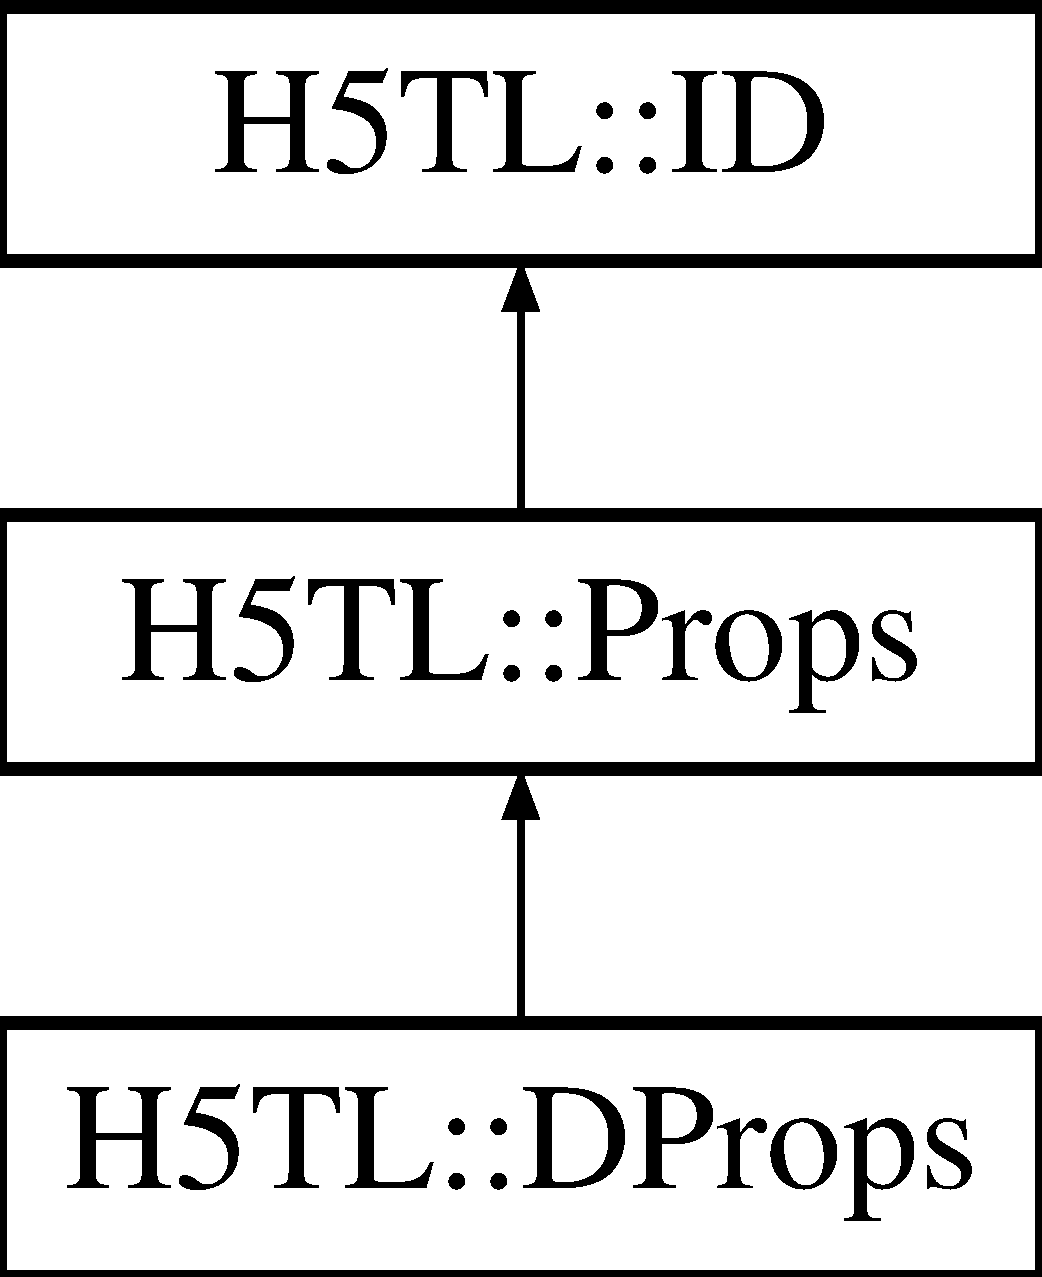
\includegraphics[height=3.000000cm]{class_h5_t_l_1_1_d_props}
\end{center}
\end{figure}
\subsection*{Public Member Functions}
\begin{DoxyCompactItemize}
\item 
\hyperlink{class_h5_t_l_1_1_d_props_a8861717b78465e2b929a8f9822a25f91}{D\-Props} ()
\item 
\hyperlink{class_h5_t_l_1_1_d_props_a4477e3f09c8df3b9235cc59a6107d18b}{D\-Props} (const \hyperlink{class_h5_t_l_1_1_d_props}{D\-Props} \&dp)
\item 
\hyperlink{class_h5_t_l_1_1_d_props_a558ee807583c289f062942f91e6bfc39}{D\-Props} (\hyperlink{class_h5_t_l_1_1_d_props}{D\-Props} \&\&dp)
\item 
virtual \hyperlink{class_h5_t_l_1_1_d_props_af24985828926acc30de48fbf2351620f}{$\sim$\-D\-Props} ()
\item 
virtual void \hyperlink{class_h5_t_l_1_1_d_props_a4e6371b21d3b981b9813709a367f7c8a}{close} ()
\item 
\hyperlink{class_h5_t_l_1_1_d_props}{D\-Props} \& \hyperlink{class_h5_t_l_1_1_d_props_a4d9c048bbe6890fb8a76f42f5e41e02c}{compact} ()
\item 
\hyperlink{class_h5_t_l_1_1_d_props}{D\-Props} \& \hyperlink{class_h5_t_l_1_1_d_props_ae93cfa78bd2904d835be0ef8c01ac328}{contiguous} ()
\item 
\hyperlink{class_h5_t_l_1_1_d_props}{D\-Props} \& \hyperlink{class_h5_t_l_1_1_d_props_ab50eedeeb4f15976869e2314cda43f28}{chunked} ()
\item 
\hyperlink{class_h5_t_l_1_1_d_props}{D\-Props} \& \hyperlink{class_h5_t_l_1_1_d_props_ae0515ee98e2bcd02c55160a33a63aabf}{chunked} (const std\-::vector$<$ hsize\-\_\-t $>$ \&chunk\-\_\-shape)
\item 
\hyperlink{class_h5_t_l_1_1_d_props}{D\-Props} \& \hyperlink{class_h5_t_l_1_1_d_props_af1283799daeee775b41effb026792b79}{chunked} (const std\-::vector$<$ hsize\-\_\-t $>$ \&data\-\_\-shape, size\-\_\-t item\-\_\-nbytes, size\-\_\-t chunk\-\_\-nbytes=0, size\-\_\-t line\-\_\-nbytes=8192)
\item 
\hyperlink{class_h5_t_l_1_1_d_props}{D\-Props} \& \hyperlink{class_h5_t_l_1_1_d_props_aa6168baf2f7cc4e171f8c65ed2e7f0e3}{deflate} (unsigned int level)
\item 
\hyperlink{class_h5_t_l_1_1_d_props}{D\-Props} \& \hyperlink{class_h5_t_l_1_1_d_props_ae8ab837067c35b714b517f9cf08c6833}{fletcher32} ()
\item 
\hyperlink{class_h5_t_l_1_1_d_props}{D\-Props} \& \hyperlink{class_h5_t_l_1_1_d_props_adf68d5443694c5a28d089efaca1ccefc}{shuffle} ()
\item 
bool \hyperlink{class_h5_t_l_1_1_d_props_a3c5536e4dd3c26da5f0fd14b85929394}{is\-\_\-chunked} () const 
\item 
std\-::vector$<$ hsize\-\_\-t $>$ \hyperlink{class_h5_t_l_1_1_d_props_a881b1504af4a748112c0193ad712f058}{chunk} () const 
\end{DoxyCompactItemize}
\subsection*{Static Public Attributes}
\begin{DoxyCompactItemize}
\item 
static const \hyperlink{class_h5_t_l_1_1_d_props}{D\-Props} \hyperlink{class_h5_t_l_1_1_d_props_a92db9269544c73f48d72be1db4256107}{D\-E\-F\-A\-U\-L\-T}
\end{DoxyCompactItemize}
\subsection*{Additional Inherited Members}


\subsection{Detailed Description}


Definition at line 361 of file H5\-T\-L.\-hpp.



\subsection{Constructor \& Destructor Documentation}
\hypertarget{class_h5_t_l_1_1_d_props_a8861717b78465e2b929a8f9822a25f91}{\index{H5\-T\-L\-::\-D\-Props@{H5\-T\-L\-::\-D\-Props}!D\-Props@{D\-Props}}
\index{D\-Props@{D\-Props}!H5TL::DProps@{H5\-T\-L\-::\-D\-Props}}
\subsubsection[{D\-Props}]{\setlength{\rightskip}{0pt plus 5cm}H5\-T\-L\-::\-D\-Props\-::\-D\-Props (
\begin{DoxyParamCaption}
{}
\end{DoxyParamCaption}
)\hspace{0.3cm}{\ttfamily [inline]}}}\label{class_h5_t_l_1_1_d_props_a8861717b78465e2b929a8f9822a25f91}


Definition at line 365 of file H5\-T\-L.\-hpp.

\hypertarget{class_h5_t_l_1_1_d_props_a4477e3f09c8df3b9235cc59a6107d18b}{\index{H5\-T\-L\-::\-D\-Props@{H5\-T\-L\-::\-D\-Props}!D\-Props@{D\-Props}}
\index{D\-Props@{D\-Props}!H5TL::DProps@{H5\-T\-L\-::\-D\-Props}}
\subsubsection[{D\-Props}]{\setlength{\rightskip}{0pt plus 5cm}H5\-T\-L\-::\-D\-Props\-::\-D\-Props (
\begin{DoxyParamCaption}
\item[{const {\bf D\-Props} \&}]{dp}
\end{DoxyParamCaption}
)\hspace{0.3cm}{\ttfamily [inline]}}}\label{class_h5_t_l_1_1_d_props_a4477e3f09c8df3b9235cc59a6107d18b}


Definition at line 366 of file H5\-T\-L.\-hpp.

\hypertarget{class_h5_t_l_1_1_d_props_a558ee807583c289f062942f91e6bfc39}{\index{H5\-T\-L\-::\-D\-Props@{H5\-T\-L\-::\-D\-Props}!D\-Props@{D\-Props}}
\index{D\-Props@{D\-Props}!H5TL::DProps@{H5\-T\-L\-::\-D\-Props}}
\subsubsection[{D\-Props}]{\setlength{\rightskip}{0pt plus 5cm}H5\-T\-L\-::\-D\-Props\-::\-D\-Props (
\begin{DoxyParamCaption}
\item[{{\bf D\-Props} \&\&}]{dp}
\end{DoxyParamCaption}
)\hspace{0.3cm}{\ttfamily [inline]}}}\label{class_h5_t_l_1_1_d_props_a558ee807583c289f062942f91e6bfc39}


Definition at line 367 of file H5\-T\-L.\-hpp.

\hypertarget{class_h5_t_l_1_1_d_props_af24985828926acc30de48fbf2351620f}{\index{H5\-T\-L\-::\-D\-Props@{H5\-T\-L\-::\-D\-Props}!$\sim$\-D\-Props@{$\sim$\-D\-Props}}
\index{$\sim$\-D\-Props@{$\sim$\-D\-Props}!H5TL::DProps@{H5\-T\-L\-::\-D\-Props}}
\subsubsection[{$\sim$\-D\-Props}]{\setlength{\rightskip}{0pt plus 5cm}virtual H5\-T\-L\-::\-D\-Props\-::$\sim$\-D\-Props (
\begin{DoxyParamCaption}
{}
\end{DoxyParamCaption}
)\hspace{0.3cm}{\ttfamily [inline]}, {\ttfamily [virtual]}}}\label{class_h5_t_l_1_1_d_props_af24985828926acc30de48fbf2351620f}


Definition at line 368 of file H5\-T\-L.\-hpp.



\subsection{Member Function Documentation}
\hypertarget{class_h5_t_l_1_1_d_props_a881b1504af4a748112c0193ad712f058}{\index{H5\-T\-L\-::\-D\-Props@{H5\-T\-L\-::\-D\-Props}!chunk@{chunk}}
\index{chunk@{chunk}!H5TL::DProps@{H5\-T\-L\-::\-D\-Props}}
\subsubsection[{chunk}]{\setlength{\rightskip}{0pt plus 5cm}std\-::vector$<$hsize\-\_\-t$>$ H5\-T\-L\-::\-D\-Props\-::chunk (
\begin{DoxyParamCaption}
{}
\end{DoxyParamCaption}
) const\hspace{0.3cm}{\ttfamily [inline]}}}\label{class_h5_t_l_1_1_d_props_a881b1504af4a748112c0193ad712f058}


Definition at line 440 of file H5\-T\-L.\-hpp.

\hypertarget{class_h5_t_l_1_1_d_props_ab50eedeeb4f15976869e2314cda43f28}{\index{H5\-T\-L\-::\-D\-Props@{H5\-T\-L\-::\-D\-Props}!chunked@{chunked}}
\index{chunked@{chunked}!H5TL::DProps@{H5\-T\-L\-::\-D\-Props}}
\subsubsection[{chunked}]{\setlength{\rightskip}{0pt plus 5cm}{\bf D\-Props}\& H5\-T\-L\-::\-D\-Props\-::chunked (
\begin{DoxyParamCaption}
{}
\end{DoxyParamCaption}
)\hspace{0.3cm}{\ttfamily [inline]}}}\label{class_h5_t_l_1_1_d_props_ab50eedeeb4f15976869e2314cda43f28}


Definition at line 384 of file H5\-T\-L.\-hpp.

\hypertarget{class_h5_t_l_1_1_d_props_ae0515ee98e2bcd02c55160a33a63aabf}{\index{H5\-T\-L\-::\-D\-Props@{H5\-T\-L\-::\-D\-Props}!chunked@{chunked}}
\index{chunked@{chunked}!H5TL::DProps@{H5\-T\-L\-::\-D\-Props}}
\subsubsection[{chunked}]{\setlength{\rightskip}{0pt plus 5cm}{\bf D\-Props}\& H5\-T\-L\-::\-D\-Props\-::chunked (
\begin{DoxyParamCaption}
\item[{const std\-::vector$<$ hsize\-\_\-t $>$ \&}]{chunk\-\_\-shape}
\end{DoxyParamCaption}
)\hspace{0.3cm}{\ttfamily [inline]}}}\label{class_h5_t_l_1_1_d_props_ae0515ee98e2bcd02c55160a33a63aabf}


Definition at line 388 of file H5\-T\-L.\-hpp.

\hypertarget{class_h5_t_l_1_1_d_props_af1283799daeee775b41effb026792b79}{\index{H5\-T\-L\-::\-D\-Props@{H5\-T\-L\-::\-D\-Props}!chunked@{chunked}}
\index{chunked@{chunked}!H5TL::DProps@{H5\-T\-L\-::\-D\-Props}}
\subsubsection[{chunked}]{\setlength{\rightskip}{0pt plus 5cm}{\bf D\-Props}\& H5\-T\-L\-::\-D\-Props\-::chunked (
\begin{DoxyParamCaption}
\item[{const std\-::vector$<$ hsize\-\_\-t $>$ \&}]{data\-\_\-shape, }
\item[{size\-\_\-t}]{item\-\_\-nbytes, }
\item[{size\-\_\-t}]{chunk\-\_\-nbytes = {\ttfamily 0}, }
\item[{size\-\_\-t}]{line\-\_\-nbytes = {\ttfamily 8192}}
\end{DoxyParamCaption}
)\hspace{0.3cm}{\ttfamily [inline]}}}\label{class_h5_t_l_1_1_d_props_af1283799daeee775b41effb026792b79}


Definition at line 392 of file H5\-T\-L.\-hpp.

\hypertarget{class_h5_t_l_1_1_d_props_a4e6371b21d3b981b9813709a367f7c8a}{\index{H5\-T\-L\-::\-D\-Props@{H5\-T\-L\-::\-D\-Props}!close@{close}}
\index{close@{close}!H5TL::DProps@{H5\-T\-L\-::\-D\-Props}}
\subsubsection[{close}]{\setlength{\rightskip}{0pt plus 5cm}virtual void H5\-T\-L\-::\-D\-Props\-::close (
\begin{DoxyParamCaption}
{}
\end{DoxyParamCaption}
)\hspace{0.3cm}{\ttfamily [inline]}, {\ttfamily [virtual]}}}\label{class_h5_t_l_1_1_d_props_a4e6371b21d3b981b9813709a367f7c8a}


Reimplemented from \hyperlink{class_h5_t_l_1_1_props_a7c0e3fcebfb68468dc1c63958d31533b}{H5\-T\-L\-::\-Props}.



Definition at line 371 of file H5\-T\-L.\-hpp.

\hypertarget{class_h5_t_l_1_1_d_props_a4d9c048bbe6890fb8a76f42f5e41e02c}{\index{H5\-T\-L\-::\-D\-Props@{H5\-T\-L\-::\-D\-Props}!compact@{compact}}
\index{compact@{compact}!H5TL::DProps@{H5\-T\-L\-::\-D\-Props}}
\subsubsection[{compact}]{\setlength{\rightskip}{0pt plus 5cm}{\bf D\-Props}\& H5\-T\-L\-::\-D\-Props\-::compact (
\begin{DoxyParamCaption}
{}
\end{DoxyParamCaption}
)\hspace{0.3cm}{\ttfamily [inline]}}}\label{class_h5_t_l_1_1_d_props_a4d9c048bbe6890fb8a76f42f5e41e02c}


Definition at line 376 of file H5\-T\-L.\-hpp.

\hypertarget{class_h5_t_l_1_1_d_props_ae93cfa78bd2904d835be0ef8c01ac328}{\index{H5\-T\-L\-::\-D\-Props@{H5\-T\-L\-::\-D\-Props}!contiguous@{contiguous}}
\index{contiguous@{contiguous}!H5TL::DProps@{H5\-T\-L\-::\-D\-Props}}
\subsubsection[{contiguous}]{\setlength{\rightskip}{0pt plus 5cm}{\bf D\-Props}\& H5\-T\-L\-::\-D\-Props\-::contiguous (
\begin{DoxyParamCaption}
{}
\end{DoxyParamCaption}
)\hspace{0.3cm}{\ttfamily [inline]}}}\label{class_h5_t_l_1_1_d_props_ae93cfa78bd2904d835be0ef8c01ac328}


Definition at line 380 of file H5\-T\-L.\-hpp.

\hypertarget{class_h5_t_l_1_1_d_props_aa6168baf2f7cc4e171f8c65ed2e7f0e3}{\index{H5\-T\-L\-::\-D\-Props@{H5\-T\-L\-::\-D\-Props}!deflate@{deflate}}
\index{deflate@{deflate}!H5TL::DProps@{H5\-T\-L\-::\-D\-Props}}
\subsubsection[{deflate}]{\setlength{\rightskip}{0pt plus 5cm}{\bf D\-Props}\& H5\-T\-L\-::\-D\-Props\-::deflate (
\begin{DoxyParamCaption}
\item[{unsigned int}]{level}
\end{DoxyParamCaption}
)\hspace{0.3cm}{\ttfamily [inline]}}}\label{class_h5_t_l_1_1_d_props_aa6168baf2f7cc4e171f8c65ed2e7f0e3}


Definition at line 425 of file H5\-T\-L.\-hpp.

\hypertarget{class_h5_t_l_1_1_d_props_ae8ab837067c35b714b517f9cf08c6833}{\index{H5\-T\-L\-::\-D\-Props@{H5\-T\-L\-::\-D\-Props}!fletcher32@{fletcher32}}
\index{fletcher32@{fletcher32}!H5TL::DProps@{H5\-T\-L\-::\-D\-Props}}
\subsubsection[{fletcher32}]{\setlength{\rightskip}{0pt plus 5cm}{\bf D\-Props}\& H5\-T\-L\-::\-D\-Props\-::fletcher32 (
\begin{DoxyParamCaption}
{}
\end{DoxyParamCaption}
)\hspace{0.3cm}{\ttfamily [inline]}}}\label{class_h5_t_l_1_1_d_props_ae8ab837067c35b714b517f9cf08c6833}


Definition at line 429 of file H5\-T\-L.\-hpp.

\hypertarget{class_h5_t_l_1_1_d_props_a3c5536e4dd3c26da5f0fd14b85929394}{\index{H5\-T\-L\-::\-D\-Props@{H5\-T\-L\-::\-D\-Props}!is\-\_\-chunked@{is\-\_\-chunked}}
\index{is\-\_\-chunked@{is\-\_\-chunked}!H5TL::DProps@{H5\-T\-L\-::\-D\-Props}}
\subsubsection[{is\-\_\-chunked}]{\setlength{\rightskip}{0pt plus 5cm}bool H5\-T\-L\-::\-D\-Props\-::is\-\_\-chunked (
\begin{DoxyParamCaption}
{}
\end{DoxyParamCaption}
) const\hspace{0.3cm}{\ttfamily [inline]}}}\label{class_h5_t_l_1_1_d_props_a3c5536e4dd3c26da5f0fd14b85929394}


Definition at line 437 of file H5\-T\-L.\-hpp.

\hypertarget{class_h5_t_l_1_1_d_props_adf68d5443694c5a28d089efaca1ccefc}{\index{H5\-T\-L\-::\-D\-Props@{H5\-T\-L\-::\-D\-Props}!shuffle@{shuffle}}
\index{shuffle@{shuffle}!H5TL::DProps@{H5\-T\-L\-::\-D\-Props}}
\subsubsection[{shuffle}]{\setlength{\rightskip}{0pt plus 5cm}{\bf D\-Props}\& H5\-T\-L\-::\-D\-Props\-::shuffle (
\begin{DoxyParamCaption}
{}
\end{DoxyParamCaption}
)\hspace{0.3cm}{\ttfamily [inline]}}}\label{class_h5_t_l_1_1_d_props_adf68d5443694c5a28d089efaca1ccefc}


Definition at line 433 of file H5\-T\-L.\-hpp.



\subsection{Member Data Documentation}
\hypertarget{class_h5_t_l_1_1_d_props_a92db9269544c73f48d72be1db4256107}{\index{H5\-T\-L\-::\-D\-Props@{H5\-T\-L\-::\-D\-Props}!D\-E\-F\-A\-U\-L\-T@{D\-E\-F\-A\-U\-L\-T}}
\index{D\-E\-F\-A\-U\-L\-T@{D\-E\-F\-A\-U\-L\-T}!H5TL::DProps@{H5\-T\-L\-::\-D\-Props}}
\subsubsection[{D\-E\-F\-A\-U\-L\-T}]{\setlength{\rightskip}{0pt plus 5cm}const {\bf D\-Props} H5\-T\-L\-::\-D\-Props\-::\-D\-E\-F\-A\-U\-L\-T\hspace{0.3cm}{\ttfamily [static]}}}\label{class_h5_t_l_1_1_d_props_a92db9269544c73f48d72be1db4256107}


Definition at line 364 of file H5\-T\-L.\-hpp.



The documentation for this class was generated from the following file\-:\begin{DoxyCompactItemize}
\item 
H5\-T\-L/\hyperlink{_h5_t_l_8hpp}{H5\-T\-L.\-hpp}\end{DoxyCompactItemize}

\hypertarget{class_h5_t_l_1_1_d_space}{\section{H5\-T\-L\-:\-:D\-Space Class Reference}
\label{class_h5_t_l_1_1_d_space}\index{H5\-T\-L\-::\-D\-Space@{H5\-T\-L\-::\-D\-Space}}
}


{\ttfamily \#include $<$H5\-T\-L.\-hpp$>$}

Inheritance diagram for H5\-T\-L\-:\-:D\-Space\-:\begin{figure}[H]
\begin{center}
\leavevmode
\includegraphics[height=2.000000cm]{class_h5_t_l_1_1_d_space}
\end{center}
\end{figure}
\subsection*{Public Member Functions}
\begin{DoxyCompactItemize}
\item 
\hyperlink{class_h5_t_l_1_1_d_space_abe4839703fc08c5851b8388ee43177ef}{D\-Space} ()
\item 
\hyperlink{class_h5_t_l_1_1_d_space_a0ba05245349237b1e42813cf4397fa32}{D\-Space} (const \hyperlink{class_h5_t_l_1_1_d_space}{D\-Space} \&ds)
\item 
\hyperlink{class_h5_t_l_1_1_d_space_af10333ae1d222213a34db2a338ae158c}{D\-Space} (\hyperlink{class_h5_t_l_1_1_d_space}{D\-Space} \&\&ds)
\item 
\hyperlink{class_h5_t_l_1_1_d_space_a0bacd841219760f82023a5c6d34d71c8}{D\-Space} (size\-\_\-t N, const hsize\-\_\-t $\ast$\hyperlink{namespace_h5_t_l_a18d3869e336e2b6a64ec318cf9890c90}{shape}, const hsize\-\_\-t $\ast$maxshape=nullptr)
\item 
{\footnotesize template$<$size\-\_\-t N$>$ }\\\hyperlink{class_h5_t_l_1_1_d_space_a361184a3052fd5fe5bd71454b244007d}{D\-Space} (const hsize\-\_\-t(\&\hyperlink{namespace_h5_t_l_a18d3869e336e2b6a64ec318cf9890c90}{shape})\mbox{[}N\mbox{]})
\item 
{\footnotesize template$<$size\-\_\-t N$>$ }\\\hyperlink{class_h5_t_l_1_1_d_space_a376a9922dbf0eb7234bb33d5e14825a9}{D\-Space} (const hsize\-\_\-t(\&\hyperlink{namespace_h5_t_l_a18d3869e336e2b6a64ec318cf9890c90}{shape})\mbox{[}N\mbox{]}, const hsize\-\_\-t(\&maxshape)\mbox{[}N\mbox{]})
\item 
\hyperlink{class_h5_t_l_1_1_d_space_a911e7f9f9398e7324c508f55fe63baaa}{D\-Space} (const std\-::vector$<$ hsize\-\_\-t $>$ \&\hyperlink{namespace_h5_t_l_a18d3869e336e2b6a64ec318cf9890c90}{shape})
\item 
\hyperlink{class_h5_t_l_1_1_d_space_aed1106ff0fb79eda9c2666b62eebc4d8}{D\-Space} (const std\-::vector$<$ hsize\-\_\-t $>$ \&\hyperlink{namespace_h5_t_l_a18d3869e336e2b6a64ec318cf9890c90}{shape}, const std\-::vector$<$ hsize\-\_\-t $>$ \&maxshape)
\item 
\hyperlink{class_h5_t_l_1_1_d_space_a7abcd0097c46b8f3252b6610bca3ebd1}{$\sim$\-D\-Space} ()
\item 
void \hyperlink{class_h5_t_l_1_1_d_space_a527298cfe321414033f52329a49e6b7a}{close} ()
\item 
\hyperlink{class_h5_t_l_1_1_d_space}{D\-Space} \& \hyperlink{class_h5_t_l_1_1_d_space_ab42688e0331b2b49d311d43dde36c31e}{select} (const \hyperlink{class_h5_t_l_1_1_selection}{Selection} \&s)
\item 
void \hyperlink{class_h5_t_l_1_1_d_space_a7557c53c7dc3b9b4e8a12cc35a438564}{extent} (const std\-::vector$<$ hsize\-\_\-t $>$ \&\hyperlink{namespace_h5_t_l_a18d3869e336e2b6a64ec318cf9890c90}{shape})
\item 
void \hyperlink{class_h5_t_l_1_1_d_space_a62a6b850d17c08da4437c6080f7c3598}{extent} (const std\-::vector$<$ hsize\-\_\-t $>$ \&\hyperlink{namespace_h5_t_l_a18d3869e336e2b6a64ec318cf9890c90}{shape}, const std\-::vector$<$ hsize\-\_\-t $>$ \&maxshape)
\item 
std\-::vector$<$ hsize\-\_\-t $>$ \hyperlink{class_h5_t_l_1_1_d_space_a217bb888d3d9666e1105a7b839f130d7}{extent} () const 
\item 
std\-::vector$<$ hsize\-\_\-t $>$ \hyperlink{class_h5_t_l_1_1_d_space_aa253d3194c386398cd3a614022226091}{max\-\_\-extent} () const 
\item 
std\-::pair$<$ std\-::vector\\*
$<$ hsize\-\_\-t $>$, std\-::vector\\*
$<$ hsize\-\_\-t $>$ $>$ \hyperlink{class_h5_t_l_1_1_d_space_a8d0637d8c3adbee551721f7fbd609de1}{extents} () const 
\end{DoxyCompactItemize}
\subsection*{Static Public Attributes}
\begin{DoxyCompactItemize}
\item 
static const size\-\_\-t \hyperlink{class_h5_t_l_1_1_d_space_aaff3fd7254edf581676b4d0a5740b80e}{M\-A\-X\-\_\-\-R\-A\-N\-K}
\item 
static const hsize\-\_\-t \hyperlink{class_h5_t_l_1_1_d_space_a2c7e4e6d7392338ff352da82243f9f21}{U\-N\-L\-I\-M\-I\-T\-E\-D}
\item 
static const hsize\-\_\-t \hyperlink{class_h5_t_l_1_1_d_space_a3f52ebf53e3a4da32927b0867a0bd8f9}{U\-N\-L}
\item 
static const \hyperlink{class_h5_t_l_1_1_d_space}{D\-Space} \hyperlink{class_h5_t_l_1_1_d_space_a0fd9cf77c7cd46e51764f71ce1e6eb11}{S\-C\-A\-L\-A\-R}
\end{DoxyCompactItemize}
\subsection*{Protected Member Functions}
\begin{DoxyCompactItemize}
\item 
\hyperlink{class_h5_t_l_1_1_d_space_add7bd418265b7dcea2e6b0fd60ea15e0}{D\-Space} (hid\-\_\-t \hyperlink{class_h5_t_l_1_1_i_d_ade483b65e8a77310b025e86b11cbc38c}{id})
\end{DoxyCompactItemize}
\subsection*{Friends}
\begin{DoxyCompactItemize}
\item 
class \hyperlink{class_h5_t_l_1_1_d_space_ab93eacb81dea8d0c21041812e61f85ab}{Dataset}
\item 
class \hyperlink{class_h5_t_l_1_1_d_space_abd4bab8f7ee748d7ea63f7f9b6248611}{Attribute}
\end{DoxyCompactItemize}
\subsection*{Additional Inherited Members}


\subsection{Detailed Description}


Definition at line 466 of file H5\-T\-L.\-hpp.



\subsection{Constructor \& Destructor Documentation}
\hypertarget{class_h5_t_l_1_1_d_space_add7bd418265b7dcea2e6b0fd60ea15e0}{\index{H5\-T\-L\-::\-D\-Space@{H5\-T\-L\-::\-D\-Space}!D\-Space@{D\-Space}}
\index{D\-Space@{D\-Space}!H5TL::DSpace@{H5\-T\-L\-::\-D\-Space}}
\subsubsection[{D\-Space}]{\setlength{\rightskip}{0pt plus 5cm}H5\-T\-L\-::\-D\-Space\-::\-D\-Space (
\begin{DoxyParamCaption}
\item[{hid\-\_\-t}]{id}
\end{DoxyParamCaption}
)\hspace{0.3cm}{\ttfamily [inline]}, {\ttfamily [protected]}}}\label{class_h5_t_l_1_1_d_space_add7bd418265b7dcea2e6b0fd60ea15e0}


Definition at line 470 of file H5\-T\-L.\-hpp.

\hypertarget{class_h5_t_l_1_1_d_space_abe4839703fc08c5851b8388ee43177ef}{\index{H5\-T\-L\-::\-D\-Space@{H5\-T\-L\-::\-D\-Space}!D\-Space@{D\-Space}}
\index{D\-Space@{D\-Space}!H5TL::DSpace@{H5\-T\-L\-::\-D\-Space}}
\subsubsection[{D\-Space}]{\setlength{\rightskip}{0pt plus 5cm}H5\-T\-L\-::\-D\-Space\-::\-D\-Space (
\begin{DoxyParamCaption}
{}
\end{DoxyParamCaption}
)\hspace{0.3cm}{\ttfamily [inline]}}}\label{class_h5_t_l_1_1_d_space_abe4839703fc08c5851b8388ee43177ef}


Definition at line 472 of file H5\-T\-L.\-hpp.

\hypertarget{class_h5_t_l_1_1_d_space_a0ba05245349237b1e42813cf4397fa32}{\index{H5\-T\-L\-::\-D\-Space@{H5\-T\-L\-::\-D\-Space}!D\-Space@{D\-Space}}
\index{D\-Space@{D\-Space}!H5TL::DSpace@{H5\-T\-L\-::\-D\-Space}}
\subsubsection[{D\-Space}]{\setlength{\rightskip}{0pt plus 5cm}H5\-T\-L\-::\-D\-Space\-::\-D\-Space (
\begin{DoxyParamCaption}
\item[{const {\bf D\-Space} \&}]{ds}
\end{DoxyParamCaption}
)\hspace{0.3cm}{\ttfamily [inline]}}}\label{class_h5_t_l_1_1_d_space_a0ba05245349237b1e42813cf4397fa32}


Definition at line 473 of file H5\-T\-L.\-hpp.

\hypertarget{class_h5_t_l_1_1_d_space_af10333ae1d222213a34db2a338ae158c}{\index{H5\-T\-L\-::\-D\-Space@{H5\-T\-L\-::\-D\-Space}!D\-Space@{D\-Space}}
\index{D\-Space@{D\-Space}!H5TL::DSpace@{H5\-T\-L\-::\-D\-Space}}
\subsubsection[{D\-Space}]{\setlength{\rightskip}{0pt plus 5cm}H5\-T\-L\-::\-D\-Space\-::\-D\-Space (
\begin{DoxyParamCaption}
\item[{{\bf D\-Space} \&\&}]{ds}
\end{DoxyParamCaption}
)\hspace{0.3cm}{\ttfamily [inline]}}}\label{class_h5_t_l_1_1_d_space_af10333ae1d222213a34db2a338ae158c}


Definition at line 474 of file H5\-T\-L.\-hpp.

\hypertarget{class_h5_t_l_1_1_d_space_a0bacd841219760f82023a5c6d34d71c8}{\index{H5\-T\-L\-::\-D\-Space@{H5\-T\-L\-::\-D\-Space}!D\-Space@{D\-Space}}
\index{D\-Space@{D\-Space}!H5TL::DSpace@{H5\-T\-L\-::\-D\-Space}}
\subsubsection[{D\-Space}]{\setlength{\rightskip}{0pt plus 5cm}H5\-T\-L\-::\-D\-Space\-::\-D\-Space (
\begin{DoxyParamCaption}
\item[{size\-\_\-t}]{N, }
\item[{const hsize\-\_\-t $\ast$}]{shape, }
\item[{const hsize\-\_\-t $\ast$}]{maxshape = {\ttfamily nullptr}}
\end{DoxyParamCaption}
)\hspace{0.3cm}{\ttfamily [inline]}}}\label{class_h5_t_l_1_1_d_space_a0bacd841219760f82023a5c6d34d71c8}


Definition at line 475 of file H5\-T\-L.\-hpp.

\hypertarget{class_h5_t_l_1_1_d_space_a361184a3052fd5fe5bd71454b244007d}{\index{H5\-T\-L\-::\-D\-Space@{H5\-T\-L\-::\-D\-Space}!D\-Space@{D\-Space}}
\index{D\-Space@{D\-Space}!H5TL::DSpace@{H5\-T\-L\-::\-D\-Space}}
\subsubsection[{D\-Space}]{\setlength{\rightskip}{0pt plus 5cm}template$<$size\-\_\-t N$>$ H5\-T\-L\-::\-D\-Space\-::\-D\-Space (
\begin{DoxyParamCaption}
\item[{const hsize\-\_\-t(\&)}]{shape\mbox{[}\-N\mbox{]}}
\end{DoxyParamCaption}
)\hspace{0.3cm}{\ttfamily [inline]}, {\ttfamily [explicit]}}}\label{class_h5_t_l_1_1_d_space_a361184a3052fd5fe5bd71454b244007d}


Definition at line 483 of file H5\-T\-L.\-hpp.

\hypertarget{class_h5_t_l_1_1_d_space_a376a9922dbf0eb7234bb33d5e14825a9}{\index{H5\-T\-L\-::\-D\-Space@{H5\-T\-L\-::\-D\-Space}!D\-Space@{D\-Space}}
\index{D\-Space@{D\-Space}!H5TL::DSpace@{H5\-T\-L\-::\-D\-Space}}
\subsubsection[{D\-Space}]{\setlength{\rightskip}{0pt plus 5cm}template$<$size\-\_\-t N$>$ H5\-T\-L\-::\-D\-Space\-::\-D\-Space (
\begin{DoxyParamCaption}
\item[{const hsize\-\_\-t(\&)}]{shape\mbox{[}\-N\mbox{]}, }
\item[{const hsize\-\_\-t(\&)}]{maxshape\mbox{[}\-N\mbox{]}}
\end{DoxyParamCaption}
)\hspace{0.3cm}{\ttfamily [inline]}}}\label{class_h5_t_l_1_1_d_space_a376a9922dbf0eb7234bb33d5e14825a9}


Definition at line 491 of file H5\-T\-L.\-hpp.

\hypertarget{class_h5_t_l_1_1_d_space_a911e7f9f9398e7324c508f55fe63baaa}{\index{H5\-T\-L\-::\-D\-Space@{H5\-T\-L\-::\-D\-Space}!D\-Space@{D\-Space}}
\index{D\-Space@{D\-Space}!H5TL::DSpace@{H5\-T\-L\-::\-D\-Space}}
\subsubsection[{D\-Space}]{\setlength{\rightskip}{0pt plus 5cm}H5\-T\-L\-::\-D\-Space\-::\-D\-Space (
\begin{DoxyParamCaption}
\item[{const std\-::vector$<$ hsize\-\_\-t $>$ \&}]{shape}
\end{DoxyParamCaption}
)\hspace{0.3cm}{\ttfamily [inline]}, {\ttfamily [explicit]}}}\label{class_h5_t_l_1_1_d_space_a911e7f9f9398e7324c508f55fe63baaa}


Definition at line 498 of file H5\-T\-L.\-hpp.

\hypertarget{class_h5_t_l_1_1_d_space_aed1106ff0fb79eda9c2666b62eebc4d8}{\index{H5\-T\-L\-::\-D\-Space@{H5\-T\-L\-::\-D\-Space}!D\-Space@{D\-Space}}
\index{D\-Space@{D\-Space}!H5TL::DSpace@{H5\-T\-L\-::\-D\-Space}}
\subsubsection[{D\-Space}]{\setlength{\rightskip}{0pt plus 5cm}H5\-T\-L\-::\-D\-Space\-::\-D\-Space (
\begin{DoxyParamCaption}
\item[{const std\-::vector$<$ hsize\-\_\-t $>$ \&}]{shape, }
\item[{const std\-::vector$<$ hsize\-\_\-t $>$ \&}]{maxshape}
\end{DoxyParamCaption}
)\hspace{0.3cm}{\ttfamily [inline]}}}\label{class_h5_t_l_1_1_d_space_aed1106ff0fb79eda9c2666b62eebc4d8}


Definition at line 506 of file H5\-T\-L.\-hpp.

\hypertarget{class_h5_t_l_1_1_d_space_a7abcd0097c46b8f3252b6610bca3ebd1}{\index{H5\-T\-L\-::\-D\-Space@{H5\-T\-L\-::\-D\-Space}!$\sim$\-D\-Space@{$\sim$\-D\-Space}}
\index{$\sim$\-D\-Space@{$\sim$\-D\-Space}!H5TL::DSpace@{H5\-T\-L\-::\-D\-Space}}
\subsubsection[{$\sim$\-D\-Space}]{\setlength{\rightskip}{0pt plus 5cm}H5\-T\-L\-::\-D\-Space\-::$\sim$\-D\-Space (
\begin{DoxyParamCaption}
{}
\end{DoxyParamCaption}
)\hspace{0.3cm}{\ttfamily [inline]}}}\label{class_h5_t_l_1_1_d_space_a7abcd0097c46b8f3252b6610bca3ebd1}


Definition at line 514 of file H5\-T\-L.\-hpp.



\subsection{Member Function Documentation}
\hypertarget{class_h5_t_l_1_1_d_space_a527298cfe321414033f52329a49e6b7a}{\index{H5\-T\-L\-::\-D\-Space@{H5\-T\-L\-::\-D\-Space}!close@{close}}
\index{close@{close}!H5TL::DSpace@{H5\-T\-L\-::\-D\-Space}}
\subsubsection[{close}]{\setlength{\rightskip}{0pt plus 5cm}void H5\-T\-L\-::\-D\-Space\-::close (
\begin{DoxyParamCaption}
{}
\end{DoxyParamCaption}
)\hspace{0.3cm}{\ttfamily [inline]}, {\ttfamily [virtual]}}}\label{class_h5_t_l_1_1_d_space_a527298cfe321414033f52329a49e6b7a}


Implements \hyperlink{class_h5_t_l_1_1_i_d_ad1a35bb991077bb094cdb0bb44339907}{H5\-T\-L\-::\-I\-D}.



Definition at line 517 of file H5\-T\-L.\-hpp.

\hypertarget{class_h5_t_l_1_1_d_space_a7557c53c7dc3b9b4e8a12cc35a438564}{\index{H5\-T\-L\-::\-D\-Space@{H5\-T\-L\-::\-D\-Space}!extent@{extent}}
\index{extent@{extent}!H5TL::DSpace@{H5\-T\-L\-::\-D\-Space}}
\subsubsection[{extent}]{\setlength{\rightskip}{0pt plus 5cm}void H5\-T\-L\-::\-D\-Space\-::extent (
\begin{DoxyParamCaption}
\item[{const std\-::vector$<$ hsize\-\_\-t $>$ \&}]{shape}
\end{DoxyParamCaption}
)\hspace{0.3cm}{\ttfamily [inline]}}}\label{class_h5_t_l_1_1_d_space_a7557c53c7dc3b9b4e8a12cc35a438564}


Definition at line 524 of file H5\-T\-L.\-hpp.

\hypertarget{class_h5_t_l_1_1_d_space_a62a6b850d17c08da4437c6080f7c3598}{\index{H5\-T\-L\-::\-D\-Space@{H5\-T\-L\-::\-D\-Space}!extent@{extent}}
\index{extent@{extent}!H5TL::DSpace@{H5\-T\-L\-::\-D\-Space}}
\subsubsection[{extent}]{\setlength{\rightskip}{0pt plus 5cm}void H5\-T\-L\-::\-D\-Space\-::extent (
\begin{DoxyParamCaption}
\item[{const std\-::vector$<$ hsize\-\_\-t $>$ \&}]{shape, }
\item[{const std\-::vector$<$ hsize\-\_\-t $>$ \&}]{maxshape}
\end{DoxyParamCaption}
)\hspace{0.3cm}{\ttfamily [inline]}}}\label{class_h5_t_l_1_1_d_space_a62a6b850d17c08da4437c6080f7c3598}


Definition at line 527 of file H5\-T\-L.\-hpp.

\hypertarget{class_h5_t_l_1_1_d_space_a217bb888d3d9666e1105a7b839f130d7}{\index{H5\-T\-L\-::\-D\-Space@{H5\-T\-L\-::\-D\-Space}!extent@{extent}}
\index{extent@{extent}!H5TL::DSpace@{H5\-T\-L\-::\-D\-Space}}
\subsubsection[{extent}]{\setlength{\rightskip}{0pt plus 5cm}std\-::vector$<$hsize\-\_\-t$>$ H5\-T\-L\-::\-D\-Space\-::extent (
\begin{DoxyParamCaption}
{}
\end{DoxyParamCaption}
) const\hspace{0.3cm}{\ttfamily [inline]}}}\label{class_h5_t_l_1_1_d_space_a217bb888d3d9666e1105a7b839f130d7}


Definition at line 530 of file H5\-T\-L.\-hpp.

\hypertarget{class_h5_t_l_1_1_d_space_a8d0637d8c3adbee551721f7fbd609de1}{\index{H5\-T\-L\-::\-D\-Space@{H5\-T\-L\-::\-D\-Space}!extents@{extents}}
\index{extents@{extents}!H5TL::DSpace@{H5\-T\-L\-::\-D\-Space}}
\subsubsection[{extents}]{\setlength{\rightskip}{0pt plus 5cm}std\-::pair$<$std\-::vector$<$hsize\-\_\-t$>$, std\-::vector$<$hsize\-\_\-t$>$ $>$ H5\-T\-L\-::\-D\-Space\-::extents (
\begin{DoxyParamCaption}
{}
\end{DoxyParamCaption}
) const\hspace{0.3cm}{\ttfamily [inline]}}}\label{class_h5_t_l_1_1_d_space_a8d0637d8c3adbee551721f7fbd609de1}


Definition at line 550 of file H5\-T\-L.\-hpp.

\hypertarget{class_h5_t_l_1_1_d_space_aa253d3194c386398cd3a614022226091}{\index{H5\-T\-L\-::\-D\-Space@{H5\-T\-L\-::\-D\-Space}!max\-\_\-extent@{max\-\_\-extent}}
\index{max\-\_\-extent@{max\-\_\-extent}!H5TL::DSpace@{H5\-T\-L\-::\-D\-Space}}
\subsubsection[{max\-\_\-extent}]{\setlength{\rightskip}{0pt plus 5cm}std\-::vector$<$hsize\-\_\-t$>$ H5\-T\-L\-::\-D\-Space\-::max\-\_\-extent (
\begin{DoxyParamCaption}
{}
\end{DoxyParamCaption}
) const\hspace{0.3cm}{\ttfamily [inline]}}}\label{class_h5_t_l_1_1_d_space_aa253d3194c386398cd3a614022226091}


Definition at line 540 of file H5\-T\-L.\-hpp.

\hypertarget{class_h5_t_l_1_1_d_space_ab42688e0331b2b49d311d43dde36c31e}{\index{H5\-T\-L\-::\-D\-Space@{H5\-T\-L\-::\-D\-Space}!select@{select}}
\index{select@{select}!H5TL::DSpace@{H5\-T\-L\-::\-D\-Space}}
\subsubsection[{select}]{\setlength{\rightskip}{0pt plus 5cm}{\bf D\-Space}\& H5\-T\-L\-::\-D\-Space\-::select (
\begin{DoxyParamCaption}
\item[{const {\bf Selection} \&}]{s}
\end{DoxyParamCaption}
)\hspace{0.3cm}{\ttfamily [inline]}}}\label{class_h5_t_l_1_1_d_space_ab42688e0331b2b49d311d43dde36c31e}


Definition at line 520 of file H5\-T\-L.\-hpp.



\subsection{Friends And Related Function Documentation}
\hypertarget{class_h5_t_l_1_1_d_space_abd4bab8f7ee748d7ea63f7f9b6248611}{\index{H5\-T\-L\-::\-D\-Space@{H5\-T\-L\-::\-D\-Space}!Attribute@{Attribute}}
\index{Attribute@{Attribute}!H5TL::DSpace@{H5\-T\-L\-::\-D\-Space}}
\subsubsection[{Attribute}]{\setlength{\rightskip}{0pt plus 5cm}friend class {\bf Attribute}\hspace{0.3cm}{\ttfamily [friend]}}}\label{class_h5_t_l_1_1_d_space_abd4bab8f7ee748d7ea63f7f9b6248611}


Definition at line 468 of file H5\-T\-L.\-hpp.

\hypertarget{class_h5_t_l_1_1_d_space_ab93eacb81dea8d0c21041812e61f85ab}{\index{H5\-T\-L\-::\-D\-Space@{H5\-T\-L\-::\-D\-Space}!Dataset@{Dataset}}
\index{Dataset@{Dataset}!H5TL::DSpace@{H5\-T\-L\-::\-D\-Space}}
\subsubsection[{Dataset}]{\setlength{\rightskip}{0pt plus 5cm}friend class {\bf Dataset}\hspace{0.3cm}{\ttfamily [friend]}}}\label{class_h5_t_l_1_1_d_space_ab93eacb81dea8d0c21041812e61f85ab}


Definition at line 467 of file H5\-T\-L.\-hpp.



\subsection{Member Data Documentation}
\hypertarget{class_h5_t_l_1_1_d_space_aaff3fd7254edf581676b4d0a5740b80e}{\index{H5\-T\-L\-::\-D\-Space@{H5\-T\-L\-::\-D\-Space}!M\-A\-X\-\_\-\-R\-A\-N\-K@{M\-A\-X\-\_\-\-R\-A\-N\-K}}
\index{M\-A\-X\-\_\-\-R\-A\-N\-K@{M\-A\-X\-\_\-\-R\-A\-N\-K}!H5TL::DSpace@{H5\-T\-L\-::\-D\-Space}}
\subsubsection[{M\-A\-X\-\_\-\-R\-A\-N\-K}]{\setlength{\rightskip}{0pt plus 5cm}const size\-\_\-t H5\-T\-L\-::\-D\-Space\-::\-M\-A\-X\-\_\-\-R\-A\-N\-K\hspace{0.3cm}{\ttfamily [static]}}}\label{class_h5_t_l_1_1_d_space_aaff3fd7254edf581676b4d0a5740b80e}


Definition at line 560 of file H5\-T\-L.\-hpp.

\hypertarget{class_h5_t_l_1_1_d_space_a0fd9cf77c7cd46e51764f71ce1e6eb11}{\index{H5\-T\-L\-::\-D\-Space@{H5\-T\-L\-::\-D\-Space}!S\-C\-A\-L\-A\-R@{S\-C\-A\-L\-A\-R}}
\index{S\-C\-A\-L\-A\-R@{S\-C\-A\-L\-A\-R}!H5TL::DSpace@{H5\-T\-L\-::\-D\-Space}}
\subsubsection[{S\-C\-A\-L\-A\-R}]{\setlength{\rightskip}{0pt plus 5cm}const {\bf D\-Space} H5\-T\-L\-::\-D\-Space\-::\-S\-C\-A\-L\-A\-R\hspace{0.3cm}{\ttfamily [static]}}}\label{class_h5_t_l_1_1_d_space_a0fd9cf77c7cd46e51764f71ce1e6eb11}


Definition at line 563 of file H5\-T\-L.\-hpp.

\hypertarget{class_h5_t_l_1_1_d_space_a3f52ebf53e3a4da32927b0867a0bd8f9}{\index{H5\-T\-L\-::\-D\-Space@{H5\-T\-L\-::\-D\-Space}!U\-N\-L@{U\-N\-L}}
\index{U\-N\-L@{U\-N\-L}!H5TL::DSpace@{H5\-T\-L\-::\-D\-Space}}
\subsubsection[{U\-N\-L}]{\setlength{\rightskip}{0pt plus 5cm}const hsize\-\_\-t H5\-T\-L\-::\-D\-Space\-::\-U\-N\-L\hspace{0.3cm}{\ttfamily [static]}}}\label{class_h5_t_l_1_1_d_space_a3f52ebf53e3a4da32927b0867a0bd8f9}


Definition at line 562 of file H5\-T\-L.\-hpp.

\hypertarget{class_h5_t_l_1_1_d_space_a2c7e4e6d7392338ff352da82243f9f21}{\index{H5\-T\-L\-::\-D\-Space@{H5\-T\-L\-::\-D\-Space}!U\-N\-L\-I\-M\-I\-T\-E\-D@{U\-N\-L\-I\-M\-I\-T\-E\-D}}
\index{U\-N\-L\-I\-M\-I\-T\-E\-D@{U\-N\-L\-I\-M\-I\-T\-E\-D}!H5TL::DSpace@{H5\-T\-L\-::\-D\-Space}}
\subsubsection[{U\-N\-L\-I\-M\-I\-T\-E\-D}]{\setlength{\rightskip}{0pt plus 5cm}const hsize\-\_\-t H5\-T\-L\-::\-D\-Space\-::\-U\-N\-L\-I\-M\-I\-T\-E\-D\hspace{0.3cm}{\ttfamily [static]}}}\label{class_h5_t_l_1_1_d_space_a2c7e4e6d7392338ff352da82243f9f21}


Definition at line 561 of file H5\-T\-L.\-hpp.



The documentation for this class was generated from the following file\-:\begin{DoxyCompactItemize}
\item 
H5\-T\-L/\hyperlink{_h5_t_l_8hpp}{H5\-T\-L.\-hpp}\end{DoxyCompactItemize}

\hypertarget{class_h5_t_l_1_1_d_type}{\section{H5\-T\-L\-:\-:D\-Type Class Reference}
\label{class_h5_t_l_1_1_d_type}\index{H5\-T\-L\-::\-D\-Type@{H5\-T\-L\-::\-D\-Type}}
}


Encapsulate an H\-D\-F5 data type object.  




{\ttfamily \#include $<$H5\-T\-L.\-hpp$>$}

Inheritance diagram for H5\-T\-L\-:\-:D\-Type\-:\begin{figure}[H]
\begin{center}
\leavevmode
\includegraphics[height=3.000000cm]{class_h5_t_l_1_1_d_type}
\end{center}
\end{figure}
\subsection*{Public Member Functions}
\begin{DoxyCompactItemize}
\item 
\hyperlink{class_h5_t_l_1_1_d_type_a5ba85ceb49042ecd7c9a536d3342a143}{D\-Type} (const \hyperlink{class_h5_t_l_1_1_d_type}{D\-Type} \&dt)
\item 
\hyperlink{class_h5_t_l_1_1_d_type_a2e4087bdb1aae026237ac05894e559b9}{D\-Type} (\hyperlink{class_h5_t_l_1_1_d_type}{D\-Type} \&\&dt)
\item 
\hyperlink{class_h5_t_l_1_1_d_type_a11fb262f22fd509d1fb047120c5b0a92}{D\-Type} (const \hyperlink{class_h5_t_l_1_1_d_type}{D\-Type} \&dt, size\-\_\-t sz)
\item 
virtual \hyperlink{class_h5_t_l_1_1_d_type_a693b78e01470174565503241195fa7d9}{$\sim$\-D\-Type} ()
\item 
void \hyperlink{class_h5_t_l_1_1_d_type_a0839ae0745f1ed4f15bfe521f14e983e}{close} ()
\item 
void \hyperlink{class_h5_t_l_1_1_d_type_a16e2caeb17c88224bb286201d1b6463c}{size} (size\-\_\-t sz)
\begin{DoxyCompactList}\small\item\em Set the size, in bytes, of the datatype. \end{DoxyCompactList}\item 
virtual size\-\_\-t \hyperlink{class_h5_t_l_1_1_d_type_a1ece4a21faeb565b63695521a0cf0767}{size} () const 
\item 
virtual bool \hyperlink{class_h5_t_l_1_1_d_type_af32cf33b4b23e8326ea7134fac1fa6b8}{operator==} (const \hyperlink{class_h5_t_l_1_1_d_type}{D\-Type} \&other) const 
\end{DoxyCompactItemize}
\subsection*{Static Public Attributes}
\begin{DoxyCompactItemize}
\item 
static const \hyperlink{class_h5_t_l_1_1_p_d_type}{P\-D\-Type} \hyperlink{class_h5_t_l_1_1_d_type_a6a438fe2e5e351a7a5f25deb4637f908}{N\-O\-N\-E}
\begin{DoxyCompactList}\small\item\em Not a valid type. \end{DoxyCompactList}\item 
static const \hyperlink{class_h5_t_l_1_1_p_d_type}{P\-D\-Type} \hyperlink{class_h5_t_l_1_1_d_type_ac2a6c1610fcc3d1a56ba67bff203f5e8}{I\-N\-T8}
\begin{DoxyCompactList}\small\item\em Native 8-\/bit signed integer type. \end{DoxyCompactList}\item 
static const \hyperlink{class_h5_t_l_1_1_p_d_type}{P\-D\-Type} \hyperlink{class_h5_t_l_1_1_d_type_a6e37c76bcf8cea8511e8ef6fbafb269b}{U\-I\-N\-T8}
\begin{DoxyCompactList}\small\item\em Native 8-\/bit unsigned integer type. \end{DoxyCompactList}\item 
static const \hyperlink{class_h5_t_l_1_1_p_d_type}{P\-D\-Type} \hyperlink{class_h5_t_l_1_1_d_type_a4f605ac6c7ba995aa5cc7f8b4b634029}{I\-N\-T16}
\begin{DoxyCompactList}\small\item\em Native 16-\/bit signed integer type. \end{DoxyCompactList}\item 
static const \hyperlink{class_h5_t_l_1_1_p_d_type}{P\-D\-Type} \hyperlink{class_h5_t_l_1_1_d_type_a95cecc3c8350b6088acbc497a89c3c10}{U\-I\-N\-T16}
\begin{DoxyCompactList}\small\item\em Native 16-\/bit unsigned integer type. \end{DoxyCompactList}\item 
static const \hyperlink{class_h5_t_l_1_1_p_d_type}{P\-D\-Type} \hyperlink{class_h5_t_l_1_1_d_type_aeac9765985f2a8195e30a84c3b23af9f}{I\-N\-T32}
\begin{DoxyCompactList}\small\item\em Native 32-\/bit signed integer type. \end{DoxyCompactList}\item 
static const \hyperlink{class_h5_t_l_1_1_p_d_type}{P\-D\-Type} \hyperlink{class_h5_t_l_1_1_d_type_a29c3994fbc6782ddfb316178fa17864d}{U\-I\-N\-T32}
\begin{DoxyCompactList}\small\item\em Native 32-\/bit unsigned integer type. \end{DoxyCompactList}\item 
static const \hyperlink{class_h5_t_l_1_1_p_d_type}{P\-D\-Type} \hyperlink{class_h5_t_l_1_1_d_type_ae8b348ef9c7faa11383fc84389ff8ffc}{I\-N\-T64}
\begin{DoxyCompactList}\small\item\em Native 64-\/bit signed integer type. \end{DoxyCompactList}\item 
static const \hyperlink{class_h5_t_l_1_1_p_d_type}{P\-D\-Type} \hyperlink{class_h5_t_l_1_1_d_type_abc95d3cc92fc398366a0a52bd21ded7a}{U\-I\-N\-T64}
\begin{DoxyCompactList}\small\item\em Native 64-\/bit unsigned integer type. \end{DoxyCompactList}\item 
static const \hyperlink{class_h5_t_l_1_1_p_d_type}{P\-D\-Type} \hyperlink{class_h5_t_l_1_1_d_type_aa7b15a197d2cc12261708d234eafecf5}{F\-L\-O\-A\-T}
\begin{DoxyCompactList}\small\item\em Native float type. \end{DoxyCompactList}\item 
static const \hyperlink{class_h5_t_l_1_1_p_d_type}{P\-D\-Type} \hyperlink{class_h5_t_l_1_1_d_type_ad17216b2872b91a3ab1ae498fec46773}{D\-O\-U\-B\-L\-E}
\begin{DoxyCompactList}\small\item\em Native double-\/precision float type. \end{DoxyCompactList}\item 
static const \hyperlink{class_h5_t_l_1_1_p_d_type}{P\-D\-Type} \hyperlink{class_h5_t_l_1_1_d_type_a261bdb031bcbd6930d09e11c53eb45d3}{S\-T\-R\-I\-N\-G}
\begin{DoxyCompactList}\small\item\em Native string character type (copy and set size for multi-\/character strings) \end{DoxyCompactList}\item 
static const \hyperlink{class_h5_t_l_1_1_p_d_type}{P\-D\-Type} \hyperlink{class_h5_t_l_1_1_d_type_aeec0653c7baf8f9c695d35ac3d5b5457}{R\-E\-F\-E\-R\-E\-N\-C\-E}
\begin{DoxyCompactList}\small\item\em H\-D\-F5 object reference type. \end{DoxyCompactList}\end{DoxyCompactItemize}
\subsection*{Protected Member Functions}
\begin{DoxyCompactItemize}
\item 
\hyperlink{class_h5_t_l_1_1_d_type_a7de5859c78eac6aacb64b355c40db270}{D\-Type} (hid\-\_\-t \hyperlink{class_h5_t_l_1_1_i_d_ade483b65e8a77310b025e86b11cbc38c}{id})
\item 
\hyperlink{class_h5_t_l_1_1_d_type_a9b125e54e616f2bd5c0c52849c6b2383}{D\-Type} (hid\-\_\-t \hyperlink{class_h5_t_l_1_1_i_d_ade483b65e8a77310b025e86b11cbc38c}{id}, size\-\_\-t sz)
\end{DoxyCompactItemize}
\subsection*{Friends}
\begin{DoxyCompactItemize}
\item 
class \hyperlink{class_h5_t_l_1_1_d_type_ab93eacb81dea8d0c21041812e61f85ab}{Dataset}
\item 
class \hyperlink{class_h5_t_l_1_1_d_type_abd4bab8f7ee748d7ea63f7f9b6248611}{Attribute}
\end{DoxyCompactItemize}
\subsection*{Additional Inherited Members}


\subsection{Detailed Description}
Encapsulate an H\-D\-F5 data type object. 

Detailed\-Description 

Definition at line 179 of file H5\-T\-L.\-hpp.



\subsection{Constructor \& Destructor Documentation}
\hypertarget{class_h5_t_l_1_1_d_type_a7de5859c78eac6aacb64b355c40db270}{\index{H5\-T\-L\-::\-D\-Type@{H5\-T\-L\-::\-D\-Type}!D\-Type@{D\-Type}}
\index{D\-Type@{D\-Type}!H5TL::DType@{H5\-T\-L\-::\-D\-Type}}
\subsubsection[{D\-Type}]{\setlength{\rightskip}{0pt plus 5cm}H5\-T\-L\-::\-D\-Type\-::\-D\-Type (
\begin{DoxyParamCaption}
\item[{hid\-\_\-t}]{id}
\end{DoxyParamCaption}
)\hspace{0.3cm}{\ttfamily [inline]}, {\ttfamily [protected]}}}\label{class_h5_t_l_1_1_d_type_a7de5859c78eac6aacb64b355c40db270}


Definition at line 183 of file H5\-T\-L.\-hpp.

\hypertarget{class_h5_t_l_1_1_d_type_a9b125e54e616f2bd5c0c52849c6b2383}{\index{H5\-T\-L\-::\-D\-Type@{H5\-T\-L\-::\-D\-Type}!D\-Type@{D\-Type}}
\index{D\-Type@{D\-Type}!H5TL::DType@{H5\-T\-L\-::\-D\-Type}}
\subsubsection[{D\-Type}]{\setlength{\rightskip}{0pt plus 5cm}H5\-T\-L\-::\-D\-Type\-::\-D\-Type (
\begin{DoxyParamCaption}
\item[{hid\-\_\-t}]{id, }
\item[{size\-\_\-t}]{sz}
\end{DoxyParamCaption}
)\hspace{0.3cm}{\ttfamily [inline]}, {\ttfamily [protected]}}}\label{class_h5_t_l_1_1_d_type_a9b125e54e616f2bd5c0c52849c6b2383}


Definition at line 184 of file H5\-T\-L.\-hpp.

\hypertarget{class_h5_t_l_1_1_d_type_a5ba85ceb49042ecd7c9a536d3342a143}{\index{H5\-T\-L\-::\-D\-Type@{H5\-T\-L\-::\-D\-Type}!D\-Type@{D\-Type}}
\index{D\-Type@{D\-Type}!H5TL::DType@{H5\-T\-L\-::\-D\-Type}}
\subsubsection[{D\-Type}]{\setlength{\rightskip}{0pt plus 5cm}H5\-T\-L\-::\-D\-Type\-::\-D\-Type (
\begin{DoxyParamCaption}
\item[{const {\bf D\-Type} \&}]{dt}
\end{DoxyParamCaption}
)\hspace{0.3cm}{\ttfamily [inline]}}}\label{class_h5_t_l_1_1_d_type_a5ba85ceb49042ecd7c9a536d3342a143}


Definition at line 188 of file H5\-T\-L.\-hpp.

\hypertarget{class_h5_t_l_1_1_d_type_a2e4087bdb1aae026237ac05894e559b9}{\index{H5\-T\-L\-::\-D\-Type@{H5\-T\-L\-::\-D\-Type}!D\-Type@{D\-Type}}
\index{D\-Type@{D\-Type}!H5TL::DType@{H5\-T\-L\-::\-D\-Type}}
\subsubsection[{D\-Type}]{\setlength{\rightskip}{0pt plus 5cm}H5\-T\-L\-::\-D\-Type\-::\-D\-Type (
\begin{DoxyParamCaption}
\item[{{\bf D\-Type} \&\&}]{dt}
\end{DoxyParamCaption}
)\hspace{0.3cm}{\ttfamily [inline]}}}\label{class_h5_t_l_1_1_d_type_a2e4087bdb1aae026237ac05894e559b9}


Definition at line 189 of file H5\-T\-L.\-hpp.

\hypertarget{class_h5_t_l_1_1_d_type_a11fb262f22fd509d1fb047120c5b0a92}{\index{H5\-T\-L\-::\-D\-Type@{H5\-T\-L\-::\-D\-Type}!D\-Type@{D\-Type}}
\index{D\-Type@{D\-Type}!H5TL::DType@{H5\-T\-L\-::\-D\-Type}}
\subsubsection[{D\-Type}]{\setlength{\rightskip}{0pt plus 5cm}H5\-T\-L\-::\-D\-Type\-::\-D\-Type (
\begin{DoxyParamCaption}
\item[{const {\bf D\-Type} \&}]{dt, }
\item[{size\-\_\-t}]{sz}
\end{DoxyParamCaption}
)\hspace{0.3cm}{\ttfamily [inline]}}}\label{class_h5_t_l_1_1_d_type_a11fb262f22fd509d1fb047120c5b0a92}


Definition at line 190 of file H5\-T\-L.\-hpp.

\hypertarget{class_h5_t_l_1_1_d_type_a693b78e01470174565503241195fa7d9}{\index{H5\-T\-L\-::\-D\-Type@{H5\-T\-L\-::\-D\-Type}!$\sim$\-D\-Type@{$\sim$\-D\-Type}}
\index{$\sim$\-D\-Type@{$\sim$\-D\-Type}!H5TL::DType@{H5\-T\-L\-::\-D\-Type}}
\subsubsection[{$\sim$\-D\-Type}]{\setlength{\rightskip}{0pt plus 5cm}virtual H5\-T\-L\-::\-D\-Type\-::$\sim$\-D\-Type (
\begin{DoxyParamCaption}
{}
\end{DoxyParamCaption}
)\hspace{0.3cm}{\ttfamily [inline]}, {\ttfamily [virtual]}}}\label{class_h5_t_l_1_1_d_type_a693b78e01470174565503241195fa7d9}


Definition at line 193 of file H5\-T\-L.\-hpp.



\subsection{Member Function Documentation}
\hypertarget{class_h5_t_l_1_1_d_type_a0839ae0745f1ed4f15bfe521f14e983e}{\index{H5\-T\-L\-::\-D\-Type@{H5\-T\-L\-::\-D\-Type}!close@{close}}
\index{close@{close}!H5TL::DType@{H5\-T\-L\-::\-D\-Type}}
\subsubsection[{close}]{\setlength{\rightskip}{0pt plus 5cm}void H5\-T\-L\-::\-D\-Type\-::close (
\begin{DoxyParamCaption}
{}
\end{DoxyParamCaption}
)\hspace{0.3cm}{\ttfamily [inline]}, {\ttfamily [virtual]}}}\label{class_h5_t_l_1_1_d_type_a0839ae0745f1ed4f15bfe521f14e983e}


Implements \hyperlink{class_h5_t_l_1_1_i_d_ad1a35bb991077bb094cdb0bb44339907}{H5\-T\-L\-::\-I\-D}.



Reimplemented in \hyperlink{class_h5_t_l_1_1_p_d_type_a85fa032de8ec7be551f92e2115743518}{H5\-T\-L\-::\-P\-D\-Type}.



Definition at line 196 of file H5\-T\-L.\-hpp.

\hypertarget{class_h5_t_l_1_1_d_type_af32cf33b4b23e8326ea7134fac1fa6b8}{\index{H5\-T\-L\-::\-D\-Type@{H5\-T\-L\-::\-D\-Type}!operator==@{operator==}}
\index{operator==@{operator==}!H5TL::DType@{H5\-T\-L\-::\-D\-Type}}
\subsubsection[{operator==}]{\setlength{\rightskip}{0pt plus 5cm}virtual bool H5\-T\-L\-::\-D\-Type\-::operator== (
\begin{DoxyParamCaption}
\item[{const {\bf D\-Type} \&}]{other}
\end{DoxyParamCaption}
) const\hspace{0.3cm}{\ttfamily [inline]}, {\ttfamily [virtual]}}}\label{class_h5_t_l_1_1_d_type_af32cf33b4b23e8326ea7134fac1fa6b8}


Definition at line 211 of file H5\-T\-L.\-hpp.

\hypertarget{class_h5_t_l_1_1_d_type_a16e2caeb17c88224bb286201d1b6463c}{\index{H5\-T\-L\-::\-D\-Type@{H5\-T\-L\-::\-D\-Type}!size@{size}}
\index{size@{size}!H5TL::DType@{H5\-T\-L\-::\-D\-Type}}
\subsubsection[{size}]{\setlength{\rightskip}{0pt plus 5cm}void H5\-T\-L\-::\-D\-Type\-::size (
\begin{DoxyParamCaption}
\item[{size\-\_\-t}]{sz}
\end{DoxyParamCaption}
)\hspace{0.3cm}{\ttfamily [inline]}}}\label{class_h5_t_l_1_1_d_type_a16e2caeb17c88224bb286201d1b6463c}


Set the size, in bytes, of the datatype. 

Set the size, in bytes, of the datatype. 
\begin{DoxyParams}[1]{Parameters}
\mbox{\tt in}  & {\em sz} & The size of the datatype, in bytes. Set to 0 for variable-\/size strings. \\
\hline
\end{DoxyParams}


Definition at line 204 of file H5\-T\-L.\-hpp.

\hypertarget{class_h5_t_l_1_1_d_type_a1ece4a21faeb565b63695521a0cf0767}{\index{H5\-T\-L\-::\-D\-Type@{H5\-T\-L\-::\-D\-Type}!size@{size}}
\index{size@{size}!H5TL::DType@{H5\-T\-L\-::\-D\-Type}}
\subsubsection[{size}]{\setlength{\rightskip}{0pt plus 5cm}virtual size\-\_\-t H5\-T\-L\-::\-D\-Type\-::size (
\begin{DoxyParamCaption}
{}
\end{DoxyParamCaption}
) const\hspace{0.3cm}{\ttfamily [inline]}, {\ttfamily [virtual]}}}\label{class_h5_t_l_1_1_d_type_a1ece4a21faeb565b63695521a0cf0767}


Definition at line 208 of file H5\-T\-L.\-hpp.



\subsection{Friends And Related Function Documentation}
\hypertarget{class_h5_t_l_1_1_d_type_abd4bab8f7ee748d7ea63f7f9b6248611}{\index{H5\-T\-L\-::\-D\-Type@{H5\-T\-L\-::\-D\-Type}!Attribute@{Attribute}}
\index{Attribute@{Attribute}!H5TL::DType@{H5\-T\-L\-::\-D\-Type}}
\subsubsection[{Attribute}]{\setlength{\rightskip}{0pt plus 5cm}friend class {\bf Attribute}\hspace{0.3cm}{\ttfamily [friend]}}}\label{class_h5_t_l_1_1_d_type_abd4bab8f7ee748d7ea63f7f9b6248611}


Definition at line 181 of file H5\-T\-L.\-hpp.

\hypertarget{class_h5_t_l_1_1_d_type_ab93eacb81dea8d0c21041812e61f85ab}{\index{H5\-T\-L\-::\-D\-Type@{H5\-T\-L\-::\-D\-Type}!Dataset@{Dataset}}
\index{Dataset@{Dataset}!H5TL::DType@{H5\-T\-L\-::\-D\-Type}}
\subsubsection[{Dataset}]{\setlength{\rightskip}{0pt plus 5cm}friend class {\bf Dataset}\hspace{0.3cm}{\ttfamily [friend]}}}\label{class_h5_t_l_1_1_d_type_ab93eacb81dea8d0c21041812e61f85ab}


Definition at line 180 of file H5\-T\-L.\-hpp.



\subsection{Member Data Documentation}
\hypertarget{class_h5_t_l_1_1_d_type_ad17216b2872b91a3ab1ae498fec46773}{\index{H5\-T\-L\-::\-D\-Type@{H5\-T\-L\-::\-D\-Type}!D\-O\-U\-B\-L\-E@{D\-O\-U\-B\-L\-E}}
\index{D\-O\-U\-B\-L\-E@{D\-O\-U\-B\-L\-E}!H5TL::DType@{H5\-T\-L\-::\-D\-Type}}
\subsubsection[{D\-O\-U\-B\-L\-E}]{\setlength{\rightskip}{0pt plus 5cm}const {\bf P\-D\-Type} H5\-T\-L\-::\-D\-Type\-::\-D\-O\-U\-B\-L\-E\hspace{0.3cm}{\ttfamily [static]}}}\label{class_h5_t_l_1_1_d_type_ad17216b2872b91a3ab1ae498fec46773}


Native double-\/precision float type. 



Definition at line 224 of file H5\-T\-L.\-hpp.

\hypertarget{class_h5_t_l_1_1_d_type_aa7b15a197d2cc12261708d234eafecf5}{\index{H5\-T\-L\-::\-D\-Type@{H5\-T\-L\-::\-D\-Type}!F\-L\-O\-A\-T@{F\-L\-O\-A\-T}}
\index{F\-L\-O\-A\-T@{F\-L\-O\-A\-T}!H5TL::DType@{H5\-T\-L\-::\-D\-Type}}
\subsubsection[{F\-L\-O\-A\-T}]{\setlength{\rightskip}{0pt plus 5cm}const {\bf P\-D\-Type} H5\-T\-L\-::\-D\-Type\-::\-F\-L\-O\-A\-T\hspace{0.3cm}{\ttfamily [static]}}}\label{class_h5_t_l_1_1_d_type_aa7b15a197d2cc12261708d234eafecf5}


Native float type. 



Definition at line 223 of file H5\-T\-L.\-hpp.

\hypertarget{class_h5_t_l_1_1_d_type_a4f605ac6c7ba995aa5cc7f8b4b634029}{\index{H5\-T\-L\-::\-D\-Type@{H5\-T\-L\-::\-D\-Type}!I\-N\-T16@{I\-N\-T16}}
\index{I\-N\-T16@{I\-N\-T16}!H5TL::DType@{H5\-T\-L\-::\-D\-Type}}
\subsubsection[{I\-N\-T16}]{\setlength{\rightskip}{0pt plus 5cm}const {\bf P\-D\-Type} H5\-T\-L\-::\-D\-Type\-::\-I\-N\-T16\hspace{0.3cm}{\ttfamily [static]}}}\label{class_h5_t_l_1_1_d_type_a4f605ac6c7ba995aa5cc7f8b4b634029}


Native 16-\/bit signed integer type. 



Definition at line 217 of file H5\-T\-L.\-hpp.

\hypertarget{class_h5_t_l_1_1_d_type_aeac9765985f2a8195e30a84c3b23af9f}{\index{H5\-T\-L\-::\-D\-Type@{H5\-T\-L\-::\-D\-Type}!I\-N\-T32@{I\-N\-T32}}
\index{I\-N\-T32@{I\-N\-T32}!H5TL::DType@{H5\-T\-L\-::\-D\-Type}}
\subsubsection[{I\-N\-T32}]{\setlength{\rightskip}{0pt plus 5cm}const {\bf P\-D\-Type} H5\-T\-L\-::\-D\-Type\-::\-I\-N\-T32\hspace{0.3cm}{\ttfamily [static]}}}\label{class_h5_t_l_1_1_d_type_aeac9765985f2a8195e30a84c3b23af9f}


Native 32-\/bit signed integer type. 



Definition at line 219 of file H5\-T\-L.\-hpp.

\hypertarget{class_h5_t_l_1_1_d_type_ae8b348ef9c7faa11383fc84389ff8ffc}{\index{H5\-T\-L\-::\-D\-Type@{H5\-T\-L\-::\-D\-Type}!I\-N\-T64@{I\-N\-T64}}
\index{I\-N\-T64@{I\-N\-T64}!H5TL::DType@{H5\-T\-L\-::\-D\-Type}}
\subsubsection[{I\-N\-T64}]{\setlength{\rightskip}{0pt plus 5cm}const {\bf P\-D\-Type} H5\-T\-L\-::\-D\-Type\-::\-I\-N\-T64\hspace{0.3cm}{\ttfamily [static]}}}\label{class_h5_t_l_1_1_d_type_ae8b348ef9c7faa11383fc84389ff8ffc}


Native 64-\/bit signed integer type. 



Definition at line 221 of file H5\-T\-L.\-hpp.

\hypertarget{class_h5_t_l_1_1_d_type_ac2a6c1610fcc3d1a56ba67bff203f5e8}{\index{H5\-T\-L\-::\-D\-Type@{H5\-T\-L\-::\-D\-Type}!I\-N\-T8@{I\-N\-T8}}
\index{I\-N\-T8@{I\-N\-T8}!H5TL::DType@{H5\-T\-L\-::\-D\-Type}}
\subsubsection[{I\-N\-T8}]{\setlength{\rightskip}{0pt plus 5cm}const {\bf P\-D\-Type} H5\-T\-L\-::\-D\-Type\-::\-I\-N\-T8\hspace{0.3cm}{\ttfamily [static]}}}\label{class_h5_t_l_1_1_d_type_ac2a6c1610fcc3d1a56ba67bff203f5e8}


Native 8-\/bit signed integer type. 



Definition at line 215 of file H5\-T\-L.\-hpp.

\hypertarget{class_h5_t_l_1_1_d_type_a6a438fe2e5e351a7a5f25deb4637f908}{\index{H5\-T\-L\-::\-D\-Type@{H5\-T\-L\-::\-D\-Type}!N\-O\-N\-E@{N\-O\-N\-E}}
\index{N\-O\-N\-E@{N\-O\-N\-E}!H5TL::DType@{H5\-T\-L\-::\-D\-Type}}
\subsubsection[{N\-O\-N\-E}]{\setlength{\rightskip}{0pt plus 5cm}const {\bf P\-D\-Type} H5\-T\-L\-::\-D\-Type\-::\-N\-O\-N\-E\hspace{0.3cm}{\ttfamily [static]}}}\label{class_h5_t_l_1_1_d_type_a6a438fe2e5e351a7a5f25deb4637f908}


Not a valid type. 



Definition at line 214 of file H5\-T\-L.\-hpp.

\hypertarget{class_h5_t_l_1_1_d_type_aeec0653c7baf8f9c695d35ac3d5b5457}{\index{H5\-T\-L\-::\-D\-Type@{H5\-T\-L\-::\-D\-Type}!R\-E\-F\-E\-R\-E\-N\-C\-E@{R\-E\-F\-E\-R\-E\-N\-C\-E}}
\index{R\-E\-F\-E\-R\-E\-N\-C\-E@{R\-E\-F\-E\-R\-E\-N\-C\-E}!H5TL::DType@{H5\-T\-L\-::\-D\-Type}}
\subsubsection[{R\-E\-F\-E\-R\-E\-N\-C\-E}]{\setlength{\rightskip}{0pt plus 5cm}const {\bf P\-D\-Type} H5\-T\-L\-::\-D\-Type\-::\-R\-E\-F\-E\-R\-E\-N\-C\-E\hspace{0.3cm}{\ttfamily [static]}}}\label{class_h5_t_l_1_1_d_type_aeec0653c7baf8f9c695d35ac3d5b5457}


H\-D\-F5 object reference type. 



Definition at line 226 of file H5\-T\-L.\-hpp.

\hypertarget{class_h5_t_l_1_1_d_type_a261bdb031bcbd6930d09e11c53eb45d3}{\index{H5\-T\-L\-::\-D\-Type@{H5\-T\-L\-::\-D\-Type}!S\-T\-R\-I\-N\-G@{S\-T\-R\-I\-N\-G}}
\index{S\-T\-R\-I\-N\-G@{S\-T\-R\-I\-N\-G}!H5TL::DType@{H5\-T\-L\-::\-D\-Type}}
\subsubsection[{S\-T\-R\-I\-N\-G}]{\setlength{\rightskip}{0pt plus 5cm}const {\bf P\-D\-Type} H5\-T\-L\-::\-D\-Type\-::\-S\-T\-R\-I\-N\-G\hspace{0.3cm}{\ttfamily [static]}}}\label{class_h5_t_l_1_1_d_type_a261bdb031bcbd6930d09e11c53eb45d3}


Native string character type (copy and set size for multi-\/character strings) 



Definition at line 225 of file H5\-T\-L.\-hpp.

\hypertarget{class_h5_t_l_1_1_d_type_a95cecc3c8350b6088acbc497a89c3c10}{\index{H5\-T\-L\-::\-D\-Type@{H5\-T\-L\-::\-D\-Type}!U\-I\-N\-T16@{U\-I\-N\-T16}}
\index{U\-I\-N\-T16@{U\-I\-N\-T16}!H5TL::DType@{H5\-T\-L\-::\-D\-Type}}
\subsubsection[{U\-I\-N\-T16}]{\setlength{\rightskip}{0pt plus 5cm}const {\bf P\-D\-Type} H5\-T\-L\-::\-D\-Type\-::\-U\-I\-N\-T16\hspace{0.3cm}{\ttfamily [static]}}}\label{class_h5_t_l_1_1_d_type_a95cecc3c8350b6088acbc497a89c3c10}


Native 16-\/bit unsigned integer type. 



Definition at line 218 of file H5\-T\-L.\-hpp.

\hypertarget{class_h5_t_l_1_1_d_type_a29c3994fbc6782ddfb316178fa17864d}{\index{H5\-T\-L\-::\-D\-Type@{H5\-T\-L\-::\-D\-Type}!U\-I\-N\-T32@{U\-I\-N\-T32}}
\index{U\-I\-N\-T32@{U\-I\-N\-T32}!H5TL::DType@{H5\-T\-L\-::\-D\-Type}}
\subsubsection[{U\-I\-N\-T32}]{\setlength{\rightskip}{0pt plus 5cm}const {\bf P\-D\-Type} H5\-T\-L\-::\-D\-Type\-::\-U\-I\-N\-T32\hspace{0.3cm}{\ttfamily [static]}}}\label{class_h5_t_l_1_1_d_type_a29c3994fbc6782ddfb316178fa17864d}


Native 32-\/bit unsigned integer type. 



Definition at line 220 of file H5\-T\-L.\-hpp.

\hypertarget{class_h5_t_l_1_1_d_type_abc95d3cc92fc398366a0a52bd21ded7a}{\index{H5\-T\-L\-::\-D\-Type@{H5\-T\-L\-::\-D\-Type}!U\-I\-N\-T64@{U\-I\-N\-T64}}
\index{U\-I\-N\-T64@{U\-I\-N\-T64}!H5TL::DType@{H5\-T\-L\-::\-D\-Type}}
\subsubsection[{U\-I\-N\-T64}]{\setlength{\rightskip}{0pt plus 5cm}const {\bf P\-D\-Type} H5\-T\-L\-::\-D\-Type\-::\-U\-I\-N\-T64\hspace{0.3cm}{\ttfamily [static]}}}\label{class_h5_t_l_1_1_d_type_abc95d3cc92fc398366a0a52bd21ded7a}


Native 64-\/bit unsigned integer type. 



Definition at line 222 of file H5\-T\-L.\-hpp.

\hypertarget{class_h5_t_l_1_1_d_type_a6e37c76bcf8cea8511e8ef6fbafb269b}{\index{H5\-T\-L\-::\-D\-Type@{H5\-T\-L\-::\-D\-Type}!U\-I\-N\-T8@{U\-I\-N\-T8}}
\index{U\-I\-N\-T8@{U\-I\-N\-T8}!H5TL::DType@{H5\-T\-L\-::\-D\-Type}}
\subsubsection[{U\-I\-N\-T8}]{\setlength{\rightskip}{0pt plus 5cm}const {\bf P\-D\-Type} H5\-T\-L\-::\-D\-Type\-::\-U\-I\-N\-T8\hspace{0.3cm}{\ttfamily [static]}}}\label{class_h5_t_l_1_1_d_type_a6e37c76bcf8cea8511e8ef6fbafb269b}


Native 8-\/bit unsigned integer type. 



Definition at line 216 of file H5\-T\-L.\-hpp.



The documentation for this class was generated from the following file\-:\begin{DoxyCompactItemize}
\item 
H5\-T\-L/\hyperlink{_h5_t_l_8hpp}{H5\-T\-L.\-hpp}\end{DoxyCompactItemize}

\hypertarget{class_h5_t_l_1_1_error_handler}{\section{H5\-T\-L\-:\-:Error\-Handler Class Reference}
\label{class_h5_t_l_1_1_error_handler}\index{H5\-T\-L\-::\-Error\-Handler@{H5\-T\-L\-::\-Error\-Handler}}
}


class for walking the H\-D\-F5 error stack.  




{\ttfamily \#include $<$H5\-T\-L.\-hpp$>$}

\subsection*{Static Public Member Functions}
\begin{DoxyCompactItemize}
\item 
static std\-::string \hyperlink{class_h5_t_l_1_1_error_handler_a21c2c116d3f151229d45bfed823185d6}{get\-\_\-error} (hid\-\_\-t es=H5\-E\-\_\-\-D\-E\-F\-A\-U\-L\-T)
\begin{DoxyCompactList}\small\item\em Return a std\-::string for the H\-D\-F5 error stack. \end{DoxyCompactList}\end{DoxyCompactItemize}
\subsection*{Protected Member Functions}
\begin{DoxyCompactItemize}
\item 
\hyperlink{class_h5_t_l_1_1_error_handler_ad45ba2e2661df16f5f78d4c1e9aeec33}{Error\-Handler} ()
\end{DoxyCompactItemize}
\subsection*{Static Protected Member Functions}
\begin{DoxyCompactItemize}
\item 
static std\-::string \hyperlink{class_h5_t_l_1_1_error_handler_a8197421bdfdd5f82b053e3737a90472d}{class\-\_\-name} (hid\-\_\-t class\-\_\-id)
\item 
static herr\-\_\-t \hyperlink{class_h5_t_l_1_1_error_handler_a76cbcca838c3ee2885dd2c5006735e1c}{append\-\_\-error} (unsigned n, const H5\-E\-\_\-error2\-\_\-t $\ast$err\-\_\-desc, void $\ast$client\-\_\-data)
\end{DoxyCompactItemize}
\subsection*{Static Protected Attributes}
\begin{DoxyCompactItemize}
\item 
static const \hyperlink{class_h5_t_l_1_1_error_handler}{Error\-Handler} \hyperlink{class_h5_t_l_1_1_error_handler_a1242321919aa0894adea386817d6a5ba}{E\-H}
\end{DoxyCompactItemize}


\subsection{Detailed Description}
class for walking the H\-D\-F5 error stack. 

Definition at line 59 of file H5\-T\-L.\-hpp.



\subsection{Constructor \& Destructor Documentation}
\hypertarget{class_h5_t_l_1_1_error_handler_ad45ba2e2661df16f5f78d4c1e9aeec33}{\index{H5\-T\-L\-::\-Error\-Handler@{H5\-T\-L\-::\-Error\-Handler}!Error\-Handler@{Error\-Handler}}
\index{Error\-Handler@{Error\-Handler}!H5TL::ErrorHandler@{H5\-T\-L\-::\-Error\-Handler}}
\subsubsection[{Error\-Handler}]{\setlength{\rightskip}{0pt plus 5cm}H5\-T\-L\-::\-Error\-Handler\-::\-Error\-Handler (
\begin{DoxyParamCaption}
{}
\end{DoxyParamCaption}
)\hspace{0.3cm}{\ttfamily [inline]}, {\ttfamily [protected]}}}\label{class_h5_t_l_1_1_error_handler_ad45ba2e2661df16f5f78d4c1e9aeec33}


Definition at line 62 of file H5\-T\-L.\-hpp.



\subsection{Member Function Documentation}
\hypertarget{class_h5_t_l_1_1_error_handler_a76cbcca838c3ee2885dd2c5006735e1c}{\index{H5\-T\-L\-::\-Error\-Handler@{H5\-T\-L\-::\-Error\-Handler}!append\-\_\-error@{append\-\_\-error}}
\index{append\-\_\-error@{append\-\_\-error}!H5TL::ErrorHandler@{H5\-T\-L\-::\-Error\-Handler}}
\subsubsection[{append\-\_\-error}]{\setlength{\rightskip}{0pt plus 5cm}static herr\-\_\-t H5\-T\-L\-::\-Error\-Handler\-::append\-\_\-error (
\begin{DoxyParamCaption}
\item[{unsigned}]{n, }
\item[{const H5\-E\-\_\-error2\-\_\-t $\ast$}]{err\-\_\-desc, }
\item[{void $\ast$}]{client\-\_\-data}
\end{DoxyParamCaption}
)\hspace{0.3cm}{\ttfamily [inline]}, {\ttfamily [static]}, {\ttfamily [protected]}}}\label{class_h5_t_l_1_1_error_handler_a76cbcca838c3ee2885dd2c5006735e1c}


Definition at line 74 of file H5\-T\-L.\-hpp.

\hypertarget{class_h5_t_l_1_1_error_handler_a8197421bdfdd5f82b053e3737a90472d}{\index{H5\-T\-L\-::\-Error\-Handler@{H5\-T\-L\-::\-Error\-Handler}!class\-\_\-name@{class\-\_\-name}}
\index{class\-\_\-name@{class\-\_\-name}!H5TL::ErrorHandler@{H5\-T\-L\-::\-Error\-Handler}}
\subsubsection[{class\-\_\-name}]{\setlength{\rightskip}{0pt plus 5cm}static std\-::string H5\-T\-L\-::\-Error\-Handler\-::class\-\_\-name (
\begin{DoxyParamCaption}
\item[{hid\-\_\-t}]{class\-\_\-id}
\end{DoxyParamCaption}
)\hspace{0.3cm}{\ttfamily [inline]}, {\ttfamily [static]}, {\ttfamily [protected]}}}\label{class_h5_t_l_1_1_error_handler_a8197421bdfdd5f82b053e3737a90472d}


Definition at line 68 of file H5\-T\-L.\-hpp.

\hypertarget{class_h5_t_l_1_1_error_handler_a21c2c116d3f151229d45bfed823185d6}{\index{H5\-T\-L\-::\-Error\-Handler@{H5\-T\-L\-::\-Error\-Handler}!get\-\_\-error@{get\-\_\-error}}
\index{get\-\_\-error@{get\-\_\-error}!H5TL::ErrorHandler@{H5\-T\-L\-::\-Error\-Handler}}
\subsubsection[{get\-\_\-error}]{\setlength{\rightskip}{0pt plus 5cm}static std\-::string H5\-T\-L\-::\-Error\-Handler\-::get\-\_\-error (
\begin{DoxyParamCaption}
\item[{hid\-\_\-t}]{es = {\ttfamily H5E\-\_\-DEFAULT}}
\end{DoxyParamCaption}
)\hspace{0.3cm}{\ttfamily [inline]}, {\ttfamily [static]}}}\label{class_h5_t_l_1_1_error_handler_a21c2c116d3f151229d45bfed823185d6}


Return a std\-::string for the H\-D\-F5 error stack. 

Walks and then clears the indicated H\-D\-F5 error stack, building a string description of the current error. 
\begin{DoxyParams}[1]{Parameters}
\mbox{\tt in}  & {\em es} & The error stack to walk, and subsequently clear. \\
\hline
\end{DoxyParams}
\begin{DoxyReturn}{Returns}
A string representation of the error stack. 
\end{DoxyReturn}


Definition at line 88 of file H5\-T\-L.\-hpp.



\subsection{Member Data Documentation}
\hypertarget{class_h5_t_l_1_1_error_handler_a1242321919aa0894adea386817d6a5ba}{\index{H5\-T\-L\-::\-Error\-Handler@{H5\-T\-L\-::\-Error\-Handler}!E\-H@{E\-H}}
\index{E\-H@{E\-H}!H5TL::ErrorHandler@{H5\-T\-L\-::\-Error\-Handler}}
\subsubsection[{E\-H}]{\setlength{\rightskip}{0pt plus 5cm}const {\bf Error\-Handler} H5\-T\-L\-::\-Error\-Handler\-::\-E\-H\hspace{0.3cm}{\ttfamily [static]}, {\ttfamily [protected]}}}\label{class_h5_t_l_1_1_error_handler_a1242321919aa0894adea386817d6a5ba}


Definition at line 66 of file H5\-T\-L.\-hpp.



The documentation for this class was generated from the following file\-:\begin{DoxyCompactItemize}
\item 
H5\-T\-L/\hyperlink{_h5_t_l_8hpp}{H5\-T\-L.\-hpp}\end{DoxyCompactItemize}

\hypertarget{class_h5_t_l_1_1_file}{\section{H5\-T\-L\-:\-:File Class Reference}
\label{class_h5_t_l_1_1_file}\index{H5\-T\-L\-::\-File@{H5\-T\-L\-::\-File}}
}


{\ttfamily \#include $<$H5\-T\-L.\-hpp$>$}

Inheritance diagram for H5\-T\-L\-:\-:File\-:\begin{figure}[H]
\begin{center}
\leavevmode
\includegraphics[height=4.000000cm]{class_h5_t_l_1_1_file}
\end{center}
\end{figure}
\subsection*{Public Types}
\begin{DoxyCompactItemize}
\item 
enum \hyperlink{class_h5_t_l_1_1_file_a19ac74cd8f7db7d836092d9354b51208}{Open\-Mode} \-: unsigned int \{ \hyperlink{class_h5_t_l_1_1_file_a19ac74cd8f7db7d836092d9354b51208a7595a9318f8f007c8177eb6129cc8a55}{T\-R\-U\-N\-C\-A\-T\-E} = H5\-F\-\_\-\-A\-C\-C\-\_\-\-T\-R\-U\-N\-C, 
\hyperlink{class_h5_t_l_1_1_file_a19ac74cd8f7db7d836092d9354b51208afcf13dfdb15f7aa5839846725365a240}{C\-R\-E\-A\-T\-E} = H5\-F\-\_\-\-A\-C\-C\-\_\-\-E\-X\-C\-L, 
\hyperlink{class_h5_t_l_1_1_file_a19ac74cd8f7db7d836092d9354b51208ab0b0c0c75d3e15b086124b605f60d753}{R\-E\-A\-D\-\_\-\-W\-R\-I\-T\-E} = H5\-F\-\_\-\-A\-C\-C\-\_\-\-R\-D\-W\-R, 
\hyperlink{class_h5_t_l_1_1_file_a19ac74cd8f7db7d836092d9354b51208a1827760549531e870388ec6866d0165e}{R\-E\-A\-D} = H5\-F\-\_\-\-A\-C\-C\-\_\-\-R\-D\-O\-N\-L\-Y
 \}
\end{DoxyCompactItemize}
\subsection*{Public Member Functions}
\begin{DoxyCompactItemize}
\item 
\hyperlink{class_h5_t_l_1_1_file_a91c89c5f48ddd0762fd39ee1e0ae73b8}{File} (const std\-::string \&name, const \hyperlink{class_h5_t_l_1_1_file_a19ac74cd8f7db7d836092d9354b51208}{Open\-Mode} \&mode=\hyperlink{class_h5_t_l_1_1_file_a19ac74cd8f7db7d836092d9354b51208ab0b0c0c75d3e15b086124b605f60d753}{R\-E\-A\-D\-\_\-\-W\-R\-I\-T\-E})
\item 
virtual \hyperlink{class_h5_t_l_1_1_file_aa05382409178af69cda0f65a13bd969f}{$\sim$\-File} ()
\item 
virtual void \hyperlink{class_h5_t_l_1_1_file_a5499e761feeab4c85ca3aba1fb218ec9}{close} ()
\end{DoxyCompactItemize}
\subsection*{Additional Inherited Members}


\subsection{Detailed Description}


Definition at line 1034 of file H5\-T\-L.\-hpp.



\subsection{Member Enumeration Documentation}
\hypertarget{class_h5_t_l_1_1_file_a19ac74cd8f7db7d836092d9354b51208}{\index{H5\-T\-L\-::\-File@{H5\-T\-L\-::\-File}!Open\-Mode@{Open\-Mode}}
\index{Open\-Mode@{Open\-Mode}!H5TL::File@{H5\-T\-L\-::\-File}}
\subsubsection[{Open\-Mode}]{\setlength{\rightskip}{0pt plus 5cm}enum {\bf H5\-T\-L\-::\-File\-::\-Open\-Mode} \-: unsigned int}}\label{class_h5_t_l_1_1_file_a19ac74cd8f7db7d836092d9354b51208}
\begin{Desc}
\item[Enumerator]\par
\begin{description}
\index{T\-R\-U\-N\-C\-A\-T\-E@{T\-R\-U\-N\-C\-A\-T\-E}!H5\-T\-L\-::\-File@{H5\-T\-L\-::\-File}}\index{H5\-T\-L\-::\-File@{H5\-T\-L\-::\-File}!T\-R\-U\-N\-C\-A\-T\-E@{T\-R\-U\-N\-C\-A\-T\-E}}\item[{\em 
\hypertarget{class_h5_t_l_1_1_file_a19ac74cd8f7db7d836092d9354b51208a7595a9318f8f007c8177eb6129cc8a55}{T\-R\-U\-N\-C\-A\-T\-E}\label{class_h5_t_l_1_1_file_a19ac74cd8f7db7d836092d9354b51208a7595a9318f8f007c8177eb6129cc8a55}
}]\index{C\-R\-E\-A\-T\-E@{C\-R\-E\-A\-T\-E}!H5\-T\-L\-::\-File@{H5\-T\-L\-::\-File}}\index{H5\-T\-L\-::\-File@{H5\-T\-L\-::\-File}!C\-R\-E\-A\-T\-E@{C\-R\-E\-A\-T\-E}}\item[{\em 
\hypertarget{class_h5_t_l_1_1_file_a19ac74cd8f7db7d836092d9354b51208afcf13dfdb15f7aa5839846725365a240}{C\-R\-E\-A\-T\-E}\label{class_h5_t_l_1_1_file_a19ac74cd8f7db7d836092d9354b51208afcf13dfdb15f7aa5839846725365a240}
}]\index{R\-E\-A\-D\-\_\-\-W\-R\-I\-T\-E@{R\-E\-A\-D\-\_\-\-W\-R\-I\-T\-E}!H5\-T\-L\-::\-File@{H5\-T\-L\-::\-File}}\index{H5\-T\-L\-::\-File@{H5\-T\-L\-::\-File}!R\-E\-A\-D\-\_\-\-W\-R\-I\-T\-E@{R\-E\-A\-D\-\_\-\-W\-R\-I\-T\-E}}\item[{\em 
\hypertarget{class_h5_t_l_1_1_file_a19ac74cd8f7db7d836092d9354b51208ab0b0c0c75d3e15b086124b605f60d753}{R\-E\-A\-D\-\_\-\-W\-R\-I\-T\-E}\label{class_h5_t_l_1_1_file_a19ac74cd8f7db7d836092d9354b51208ab0b0c0c75d3e15b086124b605f60d753}
}]\index{R\-E\-A\-D@{R\-E\-A\-D}!H5\-T\-L\-::\-File@{H5\-T\-L\-::\-File}}\index{H5\-T\-L\-::\-File@{H5\-T\-L\-::\-File}!R\-E\-A\-D@{R\-E\-A\-D}}\item[{\em 
\hypertarget{class_h5_t_l_1_1_file_a19ac74cd8f7db7d836092d9354b51208a1827760549531e870388ec6866d0165e}{R\-E\-A\-D}\label{class_h5_t_l_1_1_file_a19ac74cd8f7db7d836092d9354b51208a1827760549531e870388ec6866d0165e}
}]\end{description}
\end{Desc}


Definition at line 1036 of file H5\-T\-L.\-hpp.



\subsection{Constructor \& Destructor Documentation}
\hypertarget{class_h5_t_l_1_1_file_a91c89c5f48ddd0762fd39ee1e0ae73b8}{\index{H5\-T\-L\-::\-File@{H5\-T\-L\-::\-File}!File@{File}}
\index{File@{File}!H5TL::File@{H5\-T\-L\-::\-File}}
\subsubsection[{File}]{\setlength{\rightskip}{0pt plus 5cm}H5\-T\-L\-::\-File\-::\-File (
\begin{DoxyParamCaption}
\item[{const std\-::string \&}]{name, }
\item[{const {\bf Open\-Mode} \&}]{mode = {\ttfamily {\bf R\-E\-A\-D\-\_\-\-W\-R\-I\-T\-E}}}
\end{DoxyParamCaption}
)\hspace{0.3cm}{\ttfamily [inline]}}}\label{class_h5_t_l_1_1_file_a91c89c5f48ddd0762fd39ee1e0ae73b8}


Definition at line 1045 of file H5\-T\-L.\-hpp.

\hypertarget{class_h5_t_l_1_1_file_aa05382409178af69cda0f65a13bd969f}{\index{H5\-T\-L\-::\-File@{H5\-T\-L\-::\-File}!$\sim$\-File@{$\sim$\-File}}
\index{$\sim$\-File@{$\sim$\-File}!H5TL::File@{H5\-T\-L\-::\-File}}
\subsubsection[{$\sim$\-File}]{\setlength{\rightskip}{0pt plus 5cm}virtual H5\-T\-L\-::\-File\-::$\sim$\-File (
\begin{DoxyParamCaption}
{}
\end{DoxyParamCaption}
)\hspace{0.3cm}{\ttfamily [inline]}, {\ttfamily [virtual]}}}\label{class_h5_t_l_1_1_file_aa05382409178af69cda0f65a13bd969f}


Definition at line 1055 of file H5\-T\-L.\-hpp.



\subsection{Member Function Documentation}
\hypertarget{class_h5_t_l_1_1_file_a5499e761feeab4c85ca3aba1fb218ec9}{\index{H5\-T\-L\-::\-File@{H5\-T\-L\-::\-File}!close@{close}}
\index{close@{close}!H5TL::File@{H5\-T\-L\-::\-File}}
\subsubsection[{close}]{\setlength{\rightskip}{0pt plus 5cm}virtual void H5\-T\-L\-::\-File\-::close (
\begin{DoxyParamCaption}
{}
\end{DoxyParamCaption}
)\hspace{0.3cm}{\ttfamily [inline]}, {\ttfamily [virtual]}}}\label{class_h5_t_l_1_1_file_a5499e761feeab4c85ca3aba1fb218ec9}


Reimplemented from \hyperlink{class_h5_t_l_1_1_group_a33879ce41734238eb50b6917268d279d}{H5\-T\-L\-::\-Group}.



Definition at line 1058 of file H5\-T\-L.\-hpp.



The documentation for this class was generated from the following file\-:\begin{DoxyCompactItemize}
\item 
H5\-T\-L/\hyperlink{_h5_t_l_8hpp}{H5\-T\-L.\-hpp}\end{DoxyCompactItemize}

\hypertarget{class_h5_t_l_1_1_group}{\section{H5\-T\-L\-:\-:Group Class Reference}
\label{class_h5_t_l_1_1_group}\index{H5\-T\-L\-::\-Group@{H5\-T\-L\-::\-Group}}
}


{\ttfamily \#include $<$H5\-T\-L.\-hpp$>$}

Inheritance diagram for H5\-T\-L\-:\-:Group\-:\begin{figure}[H]
\begin{center}
\leavevmode
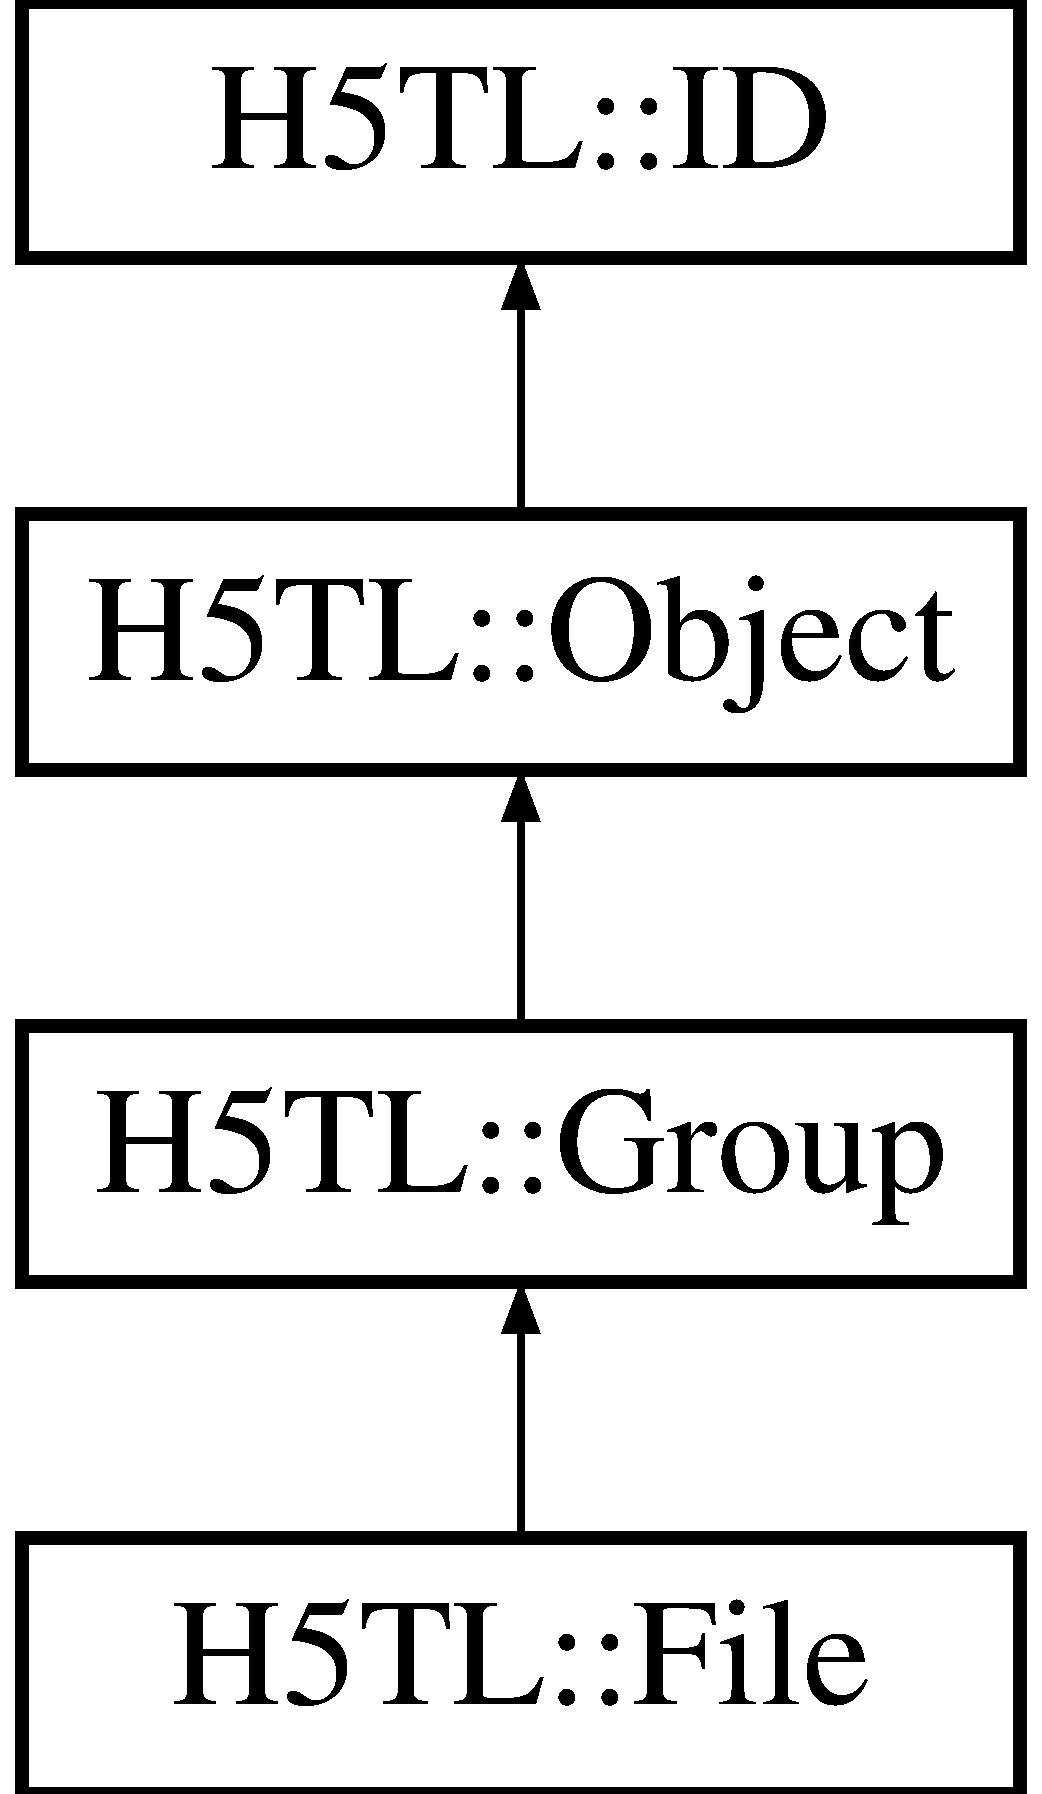
\includegraphics[height=4.000000cm]{class_h5_t_l_1_1_group}
\end{center}
\end{figure}
\subsection*{Public Member Functions}
\begin{DoxyCompactItemize}
\item 
\hyperlink{class_h5_t_l_1_1_group_a21fb4c34f51a8a56817f5a8ea1c8b9f3}{Group} (\hyperlink{class_h5_t_l_1_1_group}{Group} \&\&grp)
\item 
virtual \hyperlink{class_h5_t_l_1_1_group_a373048dcbc38705ab6439b7eb7d66a7e}{$\sim$\-Group} ()
\item 
virtual void \hyperlink{class_h5_t_l_1_1_group_a33879ce41734238eb50b6917268d279d}{close} ()
\item 
virtual bool \hyperlink{class_h5_t_l_1_1_group_ab4fbf0c28300b542e2279f5e85fb641f}{valid} (const std\-::string \&path)
\item 
virtual bool \hyperlink{class_h5_t_l_1_1_group_abbf255a903c6a9c5a5dcb33660ce0370}{exists} (const std\-::string \&path)
\item 
bool \hyperlink{class_h5_t_l_1_1_group_a7f928985e0131b63c21764136bf1a01d}{has\-Attribute} (const std\-::string \&object, const std\-::string \&attr)
\item 
\hyperlink{class_h5_t_l_1_1_group}{Group} \hyperlink{class_h5_t_l_1_1_group_ac40bee3d18aed5cc150ec47d61554ef3}{group} (const std\-::string \&name)
\item 
\hyperlink{class_h5_t_l_1_1_group}{Group} \hyperlink{class_h5_t_l_1_1_group_a84745fdcd43c75880ca4cd1e064e4ac9}{open\-Group} (const std\-::string \&name)
\item 
\hyperlink{class_h5_t_l_1_1_group}{Group} \hyperlink{class_h5_t_l_1_1_group_ab6faa3a0b9c6f9358130e1e5e4a08ad1}{create\-Group} (const std\-::string \&name)
\item 
\hyperlink{class_h5_t_l_1_1_dataset}{Dataset} \hyperlink{class_h5_t_l_1_1_group_a3bc589843f86da0a0e3c7c0382c47188}{open} (const std\-::string \&name)
\item 
\hyperlink{class_h5_t_l_1_1_dataset}{Dataset} \hyperlink{class_h5_t_l_1_1_group_aa894ff509b260d0c5d68a765a5940da9}{create} (const std\-::string \&name, const \hyperlink{class_h5_t_l_1_1_d_type}{D\-Type} \&dt, const \hyperlink{class_h5_t_l_1_1_d_space}{D\-Space} \&\hyperlink{namespace_h5_t_l_ae09d3a5b75f86dad261e807592fee081}{space}, const \hyperlink{class_h5_t_l_1_1_d_props}{D\-Props} \&props=\hyperlink{class_h5_t_l_1_1_d_props_a92db9269544c73f48d72be1db4256107}{D\-Props\-::\-D\-E\-F\-A\-U\-L\-T})
\item 
\hyperlink{class_h5_t_l_1_1_dataset}{Dataset} \hyperlink{class_h5_t_l_1_1_group_a90c193fd37dd7f35b9b62f05f830b084}{write} (const std\-::string \&name, const void $\ast$buffer, const \hyperlink{class_h5_t_l_1_1_d_type}{D\-Type} \&dt, const \hyperlink{class_h5_t_l_1_1_d_space}{D\-Space} \&\hyperlink{namespace_h5_t_l_ae09d3a5b75f86dad261e807592fee081}{space}, const \hyperlink{class_h5_t_l_1_1_d_props}{D\-Props} \&props=\hyperlink{class_h5_t_l_1_1_d_props_a92db9269544c73f48d72be1db4256107}{D\-Props\-::\-D\-E\-F\-A\-U\-L\-T})
\item 
{\footnotesize template$<$typename data\-\_\-t $>$ }\\\hyperlink{class_h5_t_l_1_1_dataset}{Dataset} \hyperlink{class_h5_t_l_1_1_group_aa7ec7b8867f7e0bcf2fb1ee7de321119}{write} (const std\-::string \&name, const data\-\_\-t \&buffer, const \hyperlink{class_h5_t_l_1_1_d_space}{D\-Space} \&\hyperlink{namespace_h5_t_l_ae09d3a5b75f86dad261e807592fee081}{space}, const \hyperlink{class_h5_t_l_1_1_d_props}{D\-Props} \&props=\hyperlink{class_h5_t_l_1_1_d_props_a92db9269544c73f48d72be1db4256107}{D\-Props\-::\-D\-E\-F\-A\-U\-L\-T})
\item 
{\footnotesize template$<$typename data\-\_\-t $>$ }\\\hyperlink{class_h5_t_l_1_1_dataset}{Dataset} \hyperlink{class_h5_t_l_1_1_group_a1acf181964e091a05491bdd07dc2acf2}{write} (const std\-::string \&name, const data\-\_\-t \&buffer, const \hyperlink{class_h5_t_l_1_1_d_props}{D\-Props} \&props=\hyperlink{class_h5_t_l_1_1_d_props_a92db9269544c73f48d72be1db4256107}{D\-Props\-::\-D\-E\-F\-A\-U\-L\-T})
\item 
\hyperlink{class_h5_t_l_1_1_dataset}{Dataset} \hyperlink{class_h5_t_l_1_1_group_ab726c68a6db6a1055085e59dfb87621f}{read} (const std\-::string \&name, void $\ast$buffer, const \hyperlink{class_h5_t_l_1_1_d_type}{D\-Type} \&buffer\-\_\-type, const \hyperlink{class_h5_t_l_1_1_d_space}{D\-Space} \&buffer\-\_\-shape, const \hyperlink{class_h5_t_l_1_1_selection}{Selection} \&selection=\hyperlink{class_h5_t_l_1_1_selection_a32d830ebff3c607e0425fa5d6ef72df0}{Selection\-::\-A\-L\-L})
\item 
\hyperlink{class_h5_t_l_1_1_dataset}{Dataset} \hyperlink{class_h5_t_l_1_1_group_a35a7440b9f212a8498da095fffa6df6d}{read} (const std\-::string \&name, void $\ast$buffer, const \hyperlink{class_h5_t_l_1_1_d_type}{D\-Type} \&buffer\-\_\-type, const \hyperlink{class_h5_t_l_1_1_d_space}{D\-Space} \&buffer\-\_\-shape, const std\-::vector$<$ hsize\-\_\-t $>$ \&offset)
\item 
{\footnotesize template$<$typename data\-\_\-t $>$ }\\\hyperlink{class_h5_t_l_1_1_dataset}{Dataset} \hyperlink{class_h5_t_l_1_1_group_ac23072a42de2e938f27e64ea0cd9d96f}{read} (const std\-::string \&name, data\-\_\-t \&buffer, const \hyperlink{class_h5_t_l_1_1_d_space}{D\-Space} \&buffer\-\_\-shape, const \hyperlink{class_h5_t_l_1_1_selection}{Selection} \&selection=\hyperlink{class_h5_t_l_1_1_selection_a32d830ebff3c607e0425fa5d6ef72df0}{Selection\-::\-A\-L\-L})
\item 
{\footnotesize template$<$typename data\-\_\-t $>$ }\\\hyperlink{class_h5_t_l_1_1_dataset}{Dataset} \hyperlink{class_h5_t_l_1_1_group_ab8333c1f74f0d82b87b0a3056b36bfa7}{read} (const std\-::string \&name, data\-\_\-t \&buffer, const \hyperlink{class_h5_t_l_1_1_d_space}{D\-Space} \&buffer\-\_\-shape, const std\-::vector$<$ hsize\-\_\-t $>$ \&offset)
\item 
{\footnotesize template$<$typename data\-\_\-t $>$ }\\\hyperlink{class_h5_t_l_1_1_dataset}{Dataset} \hyperlink{class_h5_t_l_1_1_group_a60f8bb8b3a76fa457331a375172fc716}{read} (const std\-::string \&name, data\-\_\-t \&buffer, const \hyperlink{class_h5_t_l_1_1_selection}{Selection} \&selection=\hyperlink{class_h5_t_l_1_1_selection_a32d830ebff3c607e0425fa5d6ef72df0}{Selection\-::\-A\-L\-L})
\item 
{\footnotesize template$<$typename data\-\_\-t $>$ }\\\hyperlink{class_h5_t_l_1_1_dataset}{Dataset} \hyperlink{class_h5_t_l_1_1_group_acc0a96894857a334132329442482803b}{read} (const std\-::string \&name, data\-\_\-t \&buffer, const std\-::vector$<$ hsize\-\_\-t $>$ \&offset)
\item 
{\footnotesize template$<$typename data\-\_\-t $>$ }\\\hyperlink{struct_h5_t_l_1_1adapt}{adapt}$<$ data\-\_\-t $>$\-::allocate\-\_\-return \hyperlink{class_h5_t_l_1_1_group_a3ebe23fce9aecac979096da6a71db0c5}{read} (const std\-::string \&name, const std\-::vector$<$ hsize\-\_\-t $>$ \&offset, const std\-::vector$<$ hsize\-\_\-t $>$ \&buffer\-\_\-shape)
\item 
{\footnotesize template$<$typename data\-\_\-t $>$ }\\\hyperlink{struct_h5_t_l_1_1adapt}{adapt}$<$ data\-\_\-t $>$\-::allocate\-\_\-return \hyperlink{class_h5_t_l_1_1_group_a24d333709b9200ecc94c51f4081ebd70}{read} (const std\-::string \&name)
\item 
void \hyperlink{class_h5_t_l_1_1_group_a574293c18fed3e5391267dd3c33bf81a}{create\-Hard\-Link} (const std\-::string \&name, const \hyperlink{class_h5_t_l_1_1_group}{Group} \&target\-\_\-group, const std\-::string \&target)
\item 
void \hyperlink{class_h5_t_l_1_1_group_a709506d6232025482633abcb97a4d7c5}{create\-Hard\-Link} (const std\-::string \&name, const std\-::string \&target)
\item 
void \hyperlink{class_h5_t_l_1_1_group_a2b8d910eb930a2ec45b3051452a79d73}{create\-Hard\-Link} (const std\-::string \&name, const \hyperlink{class_h5_t_l_1_1_object}{Object} \&target)
\item 
void \hyperlink{class_h5_t_l_1_1_group_a3161bd364a0f5f4df9d81619482ff559}{create\-Link} (const std\-::string \&name, const std\-::string \&target)
\item 
void \hyperlink{class_h5_t_l_1_1_group_af143a648b8feec1260727e16960afff1}{create\-Link} (const std\-::string \&name, const std\-::string \&file, const std\-::string \&target)
\end{DoxyCompactItemize}
\subsection*{Protected Member Functions}
\begin{DoxyCompactItemize}
\item 
\hyperlink{class_h5_t_l_1_1_group_ad2459b5cc9b72fe123565b5afa9c0c8a}{Group} ()
\item 
\hyperlink{class_h5_t_l_1_1_group_a23cda162d64c296d39cdd3c63551c275}{Group} (hid\-\_\-t \hyperlink{class_h5_t_l_1_1_i_d_ade483b65e8a77310b025e86b11cbc38c}{id})
\end{DoxyCompactItemize}
\subsection*{Additional Inherited Members}


\subsection{Detailed Description}


Definition at line 884 of file H5\-T\-L.\-hpp.



\subsection{Constructor \& Destructor Documentation}
\hypertarget{class_h5_t_l_1_1_group_ad2459b5cc9b72fe123565b5afa9c0c8a}{\index{H5\-T\-L\-::\-Group@{H5\-T\-L\-::\-Group}!Group@{Group}}
\index{Group@{Group}!H5TL::Group@{H5\-T\-L\-::\-Group}}
\subsubsection[{Group}]{\setlength{\rightskip}{0pt plus 5cm}H5\-T\-L\-::\-Group\-::\-Group (
\begin{DoxyParamCaption}
{}
\end{DoxyParamCaption}
)\hspace{0.3cm}{\ttfamily [inline]}, {\ttfamily [protected]}}}\label{class_h5_t_l_1_1_group_ad2459b5cc9b72fe123565b5afa9c0c8a}


Definition at line 886 of file H5\-T\-L.\-hpp.

\hypertarget{class_h5_t_l_1_1_group_a23cda162d64c296d39cdd3c63551c275}{\index{H5\-T\-L\-::\-Group@{H5\-T\-L\-::\-Group}!Group@{Group}}
\index{Group@{Group}!H5TL::Group@{H5\-T\-L\-::\-Group}}
\subsubsection[{Group}]{\setlength{\rightskip}{0pt plus 5cm}H5\-T\-L\-::\-Group\-::\-Group (
\begin{DoxyParamCaption}
\item[{hid\-\_\-t}]{id}
\end{DoxyParamCaption}
)\hspace{0.3cm}{\ttfamily [inline]}, {\ttfamily [protected]}}}\label{class_h5_t_l_1_1_group_a23cda162d64c296d39cdd3c63551c275}


Definition at line 887 of file H5\-T\-L.\-hpp.

\hypertarget{class_h5_t_l_1_1_group_a21fb4c34f51a8a56817f5a8ea1c8b9f3}{\index{H5\-T\-L\-::\-Group@{H5\-T\-L\-::\-Group}!Group@{Group}}
\index{Group@{Group}!H5TL::Group@{H5\-T\-L\-::\-Group}}
\subsubsection[{Group}]{\setlength{\rightskip}{0pt plus 5cm}H5\-T\-L\-::\-Group\-::\-Group (
\begin{DoxyParamCaption}
\item[{{\bf Group} \&\&}]{grp}
\end{DoxyParamCaption}
)\hspace{0.3cm}{\ttfamily [inline]}}}\label{class_h5_t_l_1_1_group_a21fb4c34f51a8a56817f5a8ea1c8b9f3}


Definition at line 889 of file H5\-T\-L.\-hpp.

\hypertarget{class_h5_t_l_1_1_group_a373048dcbc38705ab6439b7eb7d66a7e}{\index{H5\-T\-L\-::\-Group@{H5\-T\-L\-::\-Group}!$\sim$\-Group@{$\sim$\-Group}}
\index{$\sim$\-Group@{$\sim$\-Group}!H5TL::Group@{H5\-T\-L\-::\-Group}}
\subsubsection[{$\sim$\-Group}]{\setlength{\rightskip}{0pt plus 5cm}virtual H5\-T\-L\-::\-Group\-::$\sim$\-Group (
\begin{DoxyParamCaption}
{}
\end{DoxyParamCaption}
)\hspace{0.3cm}{\ttfamily [inline]}, {\ttfamily [virtual]}}}\label{class_h5_t_l_1_1_group_a373048dcbc38705ab6439b7eb7d66a7e}


Definition at line 890 of file H5\-T\-L.\-hpp.



\subsection{Member Function Documentation}
\hypertarget{class_h5_t_l_1_1_group_a33879ce41734238eb50b6917268d279d}{\index{H5\-T\-L\-::\-Group@{H5\-T\-L\-::\-Group}!close@{close}}
\index{close@{close}!H5TL::Group@{H5\-T\-L\-::\-Group}}
\subsubsection[{close}]{\setlength{\rightskip}{0pt plus 5cm}virtual void H5\-T\-L\-::\-Group\-::close (
\begin{DoxyParamCaption}
{}
\end{DoxyParamCaption}
)\hspace{0.3cm}{\ttfamily [inline]}, {\ttfamily [virtual]}}}\label{class_h5_t_l_1_1_group_a33879ce41734238eb50b6917268d279d}


Implements \hyperlink{class_h5_t_l_1_1_i_d_ad1a35bb991077bb094cdb0bb44339907}{H5\-T\-L\-::\-I\-D}.



Reimplemented in \hyperlink{class_h5_t_l_1_1_file_a5499e761feeab4c85ca3aba1fb218ec9}{H5\-T\-L\-::\-File}.



Definition at line 893 of file H5\-T\-L.\-hpp.

\hypertarget{class_h5_t_l_1_1_group_aa894ff509b260d0c5d68a765a5940da9}{\index{H5\-T\-L\-::\-Group@{H5\-T\-L\-::\-Group}!create@{create}}
\index{create@{create}!H5TL::Group@{H5\-T\-L\-::\-Group}}
\subsubsection[{create}]{\setlength{\rightskip}{0pt plus 5cm}{\bf Dataset} H5\-T\-L\-::\-Group\-::create (
\begin{DoxyParamCaption}
\item[{const std\-::string \&}]{name, }
\item[{const {\bf D\-Type} \&}]{dt, }
\item[{const {\bf D\-Space} \&}]{space, }
\item[{const {\bf D\-Props} \&}]{props = {\ttfamily {\bf D\-Props\-::\-D\-E\-F\-A\-U\-L\-T}}}
\end{DoxyParamCaption}
)\hspace{0.3cm}{\ttfamily [inline]}}}\label{class_h5_t_l_1_1_group_aa894ff509b260d0c5d68a765a5940da9}


Definition at line 951 of file H5\-T\-L.\-hpp.

\hypertarget{class_h5_t_l_1_1_group_ab6faa3a0b9c6f9358130e1e5e4a08ad1}{\index{H5\-T\-L\-::\-Group@{H5\-T\-L\-::\-Group}!create\-Group@{create\-Group}}
\index{create\-Group@{create\-Group}!H5TL::Group@{H5\-T\-L\-::\-Group}}
\subsubsection[{create\-Group}]{\setlength{\rightskip}{0pt plus 5cm}{\bf Group} H5\-T\-L\-::\-Group\-::create\-Group (
\begin{DoxyParamCaption}
\item[{const std\-::string \&}]{name}
\end{DoxyParamCaption}
)\hspace{0.3cm}{\ttfamily [inline]}}}\label{class_h5_t_l_1_1_group_ab6faa3a0b9c6f9358130e1e5e4a08ad1}


Definition at line 945 of file H5\-T\-L.\-hpp.

\hypertarget{class_h5_t_l_1_1_group_a574293c18fed3e5391267dd3c33bf81a}{\index{H5\-T\-L\-::\-Group@{H5\-T\-L\-::\-Group}!create\-Hard\-Link@{create\-Hard\-Link}}
\index{create\-Hard\-Link@{create\-Hard\-Link}!H5TL::Group@{H5\-T\-L\-::\-Group}}
\subsubsection[{create\-Hard\-Link}]{\setlength{\rightskip}{0pt plus 5cm}void H5\-T\-L\-::\-Group\-::create\-Hard\-Link (
\begin{DoxyParamCaption}
\item[{const std\-::string \&}]{name, }
\item[{const {\bf Group} \&}]{target\-\_\-group, }
\item[{const std\-::string \&}]{target}
\end{DoxyParamCaption}
)\hspace{0.3cm}{\ttfamily [inline]}}}\label{class_h5_t_l_1_1_group_a574293c18fed3e5391267dd3c33bf81a}


Definition at line 1016 of file H5\-T\-L.\-hpp.

\hypertarget{class_h5_t_l_1_1_group_a709506d6232025482633abcb97a4d7c5}{\index{H5\-T\-L\-::\-Group@{H5\-T\-L\-::\-Group}!create\-Hard\-Link@{create\-Hard\-Link}}
\index{create\-Hard\-Link@{create\-Hard\-Link}!H5TL::Group@{H5\-T\-L\-::\-Group}}
\subsubsection[{create\-Hard\-Link}]{\setlength{\rightskip}{0pt plus 5cm}void H5\-T\-L\-::\-Group\-::create\-Hard\-Link (
\begin{DoxyParamCaption}
\item[{const std\-::string \&}]{name, }
\item[{const std\-::string \&}]{target}
\end{DoxyParamCaption}
)\hspace{0.3cm}{\ttfamily [inline]}}}\label{class_h5_t_l_1_1_group_a709506d6232025482633abcb97a4d7c5}


Definition at line 1019 of file H5\-T\-L.\-hpp.

\hypertarget{class_h5_t_l_1_1_group_a2b8d910eb930a2ec45b3051452a79d73}{\index{H5\-T\-L\-::\-Group@{H5\-T\-L\-::\-Group}!create\-Hard\-Link@{create\-Hard\-Link}}
\index{create\-Hard\-Link@{create\-Hard\-Link}!H5TL::Group@{H5\-T\-L\-::\-Group}}
\subsubsection[{create\-Hard\-Link}]{\setlength{\rightskip}{0pt plus 5cm}void H5\-T\-L\-::\-Group\-::create\-Hard\-Link (
\begin{DoxyParamCaption}
\item[{const std\-::string \&}]{name, }
\item[{const {\bf Object} \&}]{target}
\end{DoxyParamCaption}
)\hspace{0.3cm}{\ttfamily [inline]}}}\label{class_h5_t_l_1_1_group_a2b8d910eb930a2ec45b3051452a79d73}


Definition at line 1022 of file H5\-T\-L.\-hpp.

\hypertarget{class_h5_t_l_1_1_group_a3161bd364a0f5f4df9d81619482ff559}{\index{H5\-T\-L\-::\-Group@{H5\-T\-L\-::\-Group}!create\-Link@{create\-Link}}
\index{create\-Link@{create\-Link}!H5TL::Group@{H5\-T\-L\-::\-Group}}
\subsubsection[{create\-Link}]{\setlength{\rightskip}{0pt plus 5cm}void H5\-T\-L\-::\-Group\-::create\-Link (
\begin{DoxyParamCaption}
\item[{const std\-::string \&}]{name, }
\item[{const std\-::string \&}]{target}
\end{DoxyParamCaption}
)\hspace{0.3cm}{\ttfamily [inline]}}}\label{class_h5_t_l_1_1_group_a3161bd364a0f5f4df9d81619482ff559}


Definition at line 1025 of file H5\-T\-L.\-hpp.

\hypertarget{class_h5_t_l_1_1_group_af143a648b8feec1260727e16960afff1}{\index{H5\-T\-L\-::\-Group@{H5\-T\-L\-::\-Group}!create\-Link@{create\-Link}}
\index{create\-Link@{create\-Link}!H5TL::Group@{H5\-T\-L\-::\-Group}}
\subsubsection[{create\-Link}]{\setlength{\rightskip}{0pt plus 5cm}void H5\-T\-L\-::\-Group\-::create\-Link (
\begin{DoxyParamCaption}
\item[{const std\-::string \&}]{name, }
\item[{const std\-::string \&}]{file, }
\item[{const std\-::string \&}]{target}
\end{DoxyParamCaption}
)\hspace{0.3cm}{\ttfamily [inline]}}}\label{class_h5_t_l_1_1_group_af143a648b8feec1260727e16960afff1}


Definition at line 1028 of file H5\-T\-L.\-hpp.

\hypertarget{class_h5_t_l_1_1_group_abbf255a903c6a9c5a5dcb33660ce0370}{\index{H5\-T\-L\-::\-Group@{H5\-T\-L\-::\-Group}!exists@{exists}}
\index{exists@{exists}!H5TL::Group@{H5\-T\-L\-::\-Group}}
\subsubsection[{exists}]{\setlength{\rightskip}{0pt plus 5cm}virtual bool H5\-T\-L\-::\-Group\-::exists (
\begin{DoxyParamCaption}
\item[{const std\-::string \&}]{path}
\end{DoxyParamCaption}
)\hspace{0.3cm}{\ttfamily [inline]}, {\ttfamily [virtual]}}}\label{class_h5_t_l_1_1_group_abbf255a903c6a9c5a5dcb33660ce0370}


Definition at line 928 of file H5\-T\-L.\-hpp.

\hypertarget{class_h5_t_l_1_1_group_ac40bee3d18aed5cc150ec47d61554ef3}{\index{H5\-T\-L\-::\-Group@{H5\-T\-L\-::\-Group}!group@{group}}
\index{group@{group}!H5TL::Group@{H5\-T\-L\-::\-Group}}
\subsubsection[{group}]{\setlength{\rightskip}{0pt plus 5cm}{\bf Group} H5\-T\-L\-::\-Group\-::group (
\begin{DoxyParamCaption}
\item[{const std\-::string \&}]{name}
\end{DoxyParamCaption}
)\hspace{0.3cm}{\ttfamily [inline]}}}\label{class_h5_t_l_1_1_group_ac40bee3d18aed5cc150ec47d61554ef3}


Definition at line 936 of file H5\-T\-L.\-hpp.

\hypertarget{class_h5_t_l_1_1_group_a7f928985e0131b63c21764136bf1a01d}{\index{H5\-T\-L\-::\-Group@{H5\-T\-L\-::\-Group}!has\-Attribute@{has\-Attribute}}
\index{has\-Attribute@{has\-Attribute}!H5TL::Group@{H5\-T\-L\-::\-Group}}
\subsubsection[{has\-Attribute}]{\setlength{\rightskip}{0pt plus 5cm}bool H5\-T\-L\-::\-Group\-::has\-Attribute (
\begin{DoxyParamCaption}
\item[{const std\-::string \&}]{object, }
\item[{const std\-::string \&}]{attr}
\end{DoxyParamCaption}
)\hspace{0.3cm}{\ttfamily [inline]}}}\label{class_h5_t_l_1_1_group_a7f928985e0131b63c21764136bf1a01d}


Definition at line 933 of file H5\-T\-L.\-hpp.

\hypertarget{class_h5_t_l_1_1_group_a3bc589843f86da0a0e3c7c0382c47188}{\index{H5\-T\-L\-::\-Group@{H5\-T\-L\-::\-Group}!open@{open}}
\index{open@{open}!H5TL::Group@{H5\-T\-L\-::\-Group}}
\subsubsection[{open}]{\setlength{\rightskip}{0pt plus 5cm}{\bf Dataset} H5\-T\-L\-::\-Group\-::open (
\begin{DoxyParamCaption}
\item[{const std\-::string \&}]{name}
\end{DoxyParamCaption}
)\hspace{0.3cm}{\ttfamily [inline]}}}\label{class_h5_t_l_1_1_group_a3bc589843f86da0a0e3c7c0382c47188}


Definition at line 948 of file H5\-T\-L.\-hpp.

\hypertarget{class_h5_t_l_1_1_group_a84745fdcd43c75880ca4cd1e064e4ac9}{\index{H5\-T\-L\-::\-Group@{H5\-T\-L\-::\-Group}!open\-Group@{open\-Group}}
\index{open\-Group@{open\-Group}!H5TL::Group@{H5\-T\-L\-::\-Group}}
\subsubsection[{open\-Group}]{\setlength{\rightskip}{0pt plus 5cm}{\bf Group} H5\-T\-L\-::\-Group\-::open\-Group (
\begin{DoxyParamCaption}
\item[{const std\-::string \&}]{name}
\end{DoxyParamCaption}
)\hspace{0.3cm}{\ttfamily [inline]}}}\label{class_h5_t_l_1_1_group_a84745fdcd43c75880ca4cd1e064e4ac9}


Definition at line 942 of file H5\-T\-L.\-hpp.

\hypertarget{class_h5_t_l_1_1_group_ab726c68a6db6a1055085e59dfb87621f}{\index{H5\-T\-L\-::\-Group@{H5\-T\-L\-::\-Group}!read@{read}}
\index{read@{read}!H5TL::Group@{H5\-T\-L\-::\-Group}}
\subsubsection[{read}]{\setlength{\rightskip}{0pt plus 5cm}{\bf Dataset} H5\-T\-L\-::\-Group\-::read (
\begin{DoxyParamCaption}
\item[{const std\-::string \&}]{name, }
\item[{void $\ast$}]{buffer, }
\item[{const {\bf D\-Type} \&}]{buffer\-\_\-type, }
\item[{const {\bf D\-Space} \&}]{buffer\-\_\-shape, }
\item[{const {\bf Selection} \&}]{selection = {\ttfamily {\bf Selection\-::\-A\-L\-L}}}
\end{DoxyParamCaption}
)\hspace{0.3cm}{\ttfamily [inline]}}}\label{class_h5_t_l_1_1_group_ab726c68a6db6a1055085e59dfb87621f}


Definition at line 978 of file H5\-T\-L.\-hpp.

\hypertarget{class_h5_t_l_1_1_group_a35a7440b9f212a8498da095fffa6df6d}{\index{H5\-T\-L\-::\-Group@{H5\-T\-L\-::\-Group}!read@{read}}
\index{read@{read}!H5TL::Group@{H5\-T\-L\-::\-Group}}
\subsubsection[{read}]{\setlength{\rightskip}{0pt plus 5cm}{\bf Dataset} H5\-T\-L\-::\-Group\-::read (
\begin{DoxyParamCaption}
\item[{const std\-::string \&}]{name, }
\item[{void $\ast$}]{buffer, }
\item[{const {\bf D\-Type} \&}]{buffer\-\_\-type, }
\item[{const {\bf D\-Space} \&}]{buffer\-\_\-shape, }
\item[{const std\-::vector$<$ hsize\-\_\-t $>$ \&}]{offset}
\end{DoxyParamCaption}
)\hspace{0.3cm}{\ttfamily [inline]}}}\label{class_h5_t_l_1_1_group_a35a7440b9f212a8498da095fffa6df6d}


Definition at line 983 of file H5\-T\-L.\-hpp.

\hypertarget{class_h5_t_l_1_1_group_ac23072a42de2e938f27e64ea0cd9d96f}{\index{H5\-T\-L\-::\-Group@{H5\-T\-L\-::\-Group}!read@{read}}
\index{read@{read}!H5TL::Group@{H5\-T\-L\-::\-Group}}
\subsubsection[{read}]{\setlength{\rightskip}{0pt plus 5cm}template$<$typename data\-\_\-t $>$ {\bf Dataset} H5\-T\-L\-::\-Group\-::read (
\begin{DoxyParamCaption}
\item[{const std\-::string \&}]{name, }
\item[{data\-\_\-t \&}]{buffer, }
\item[{const {\bf D\-Space} \&}]{buffer\-\_\-shape, }
\item[{const {\bf Selection} \&}]{selection = {\ttfamily {\bf Selection\-::\-A\-L\-L}}}
\end{DoxyParamCaption}
)\hspace{0.3cm}{\ttfamily [inline]}}}\label{class_h5_t_l_1_1_group_ac23072a42de2e938f27e64ea0cd9d96f}


Definition at line 987 of file H5\-T\-L.\-hpp.

\hypertarget{class_h5_t_l_1_1_group_ab8333c1f74f0d82b87b0a3056b36bfa7}{\index{H5\-T\-L\-::\-Group@{H5\-T\-L\-::\-Group}!read@{read}}
\index{read@{read}!H5TL::Group@{H5\-T\-L\-::\-Group}}
\subsubsection[{read}]{\setlength{\rightskip}{0pt plus 5cm}template$<$typename data\-\_\-t $>$ {\bf Dataset} H5\-T\-L\-::\-Group\-::read (
\begin{DoxyParamCaption}
\item[{const std\-::string \&}]{name, }
\item[{data\-\_\-t \&}]{buffer, }
\item[{const {\bf D\-Space} \&}]{buffer\-\_\-shape, }
\item[{const std\-::vector$<$ hsize\-\_\-t $>$ \&}]{offset}
\end{DoxyParamCaption}
)\hspace{0.3cm}{\ttfamily [inline]}}}\label{class_h5_t_l_1_1_group_ab8333c1f74f0d82b87b0a3056b36bfa7}


Definition at line 991 of file H5\-T\-L.\-hpp.

\hypertarget{class_h5_t_l_1_1_group_a60f8bb8b3a76fa457331a375172fc716}{\index{H5\-T\-L\-::\-Group@{H5\-T\-L\-::\-Group}!read@{read}}
\index{read@{read}!H5TL::Group@{H5\-T\-L\-::\-Group}}
\subsubsection[{read}]{\setlength{\rightskip}{0pt plus 5cm}template$<$typename data\-\_\-t $>$ {\bf Dataset} H5\-T\-L\-::\-Group\-::read (
\begin{DoxyParamCaption}
\item[{const std\-::string \&}]{name, }
\item[{data\-\_\-t \&}]{buffer, }
\item[{const {\bf Selection} \&}]{selection = {\ttfamily {\bf Selection\-::\-A\-L\-L}}}
\end{DoxyParamCaption}
)\hspace{0.3cm}{\ttfamily [inline]}}}\label{class_h5_t_l_1_1_group_a60f8bb8b3a76fa457331a375172fc716}


Definition at line 995 of file H5\-T\-L.\-hpp.

\hypertarget{class_h5_t_l_1_1_group_acc0a96894857a334132329442482803b}{\index{H5\-T\-L\-::\-Group@{H5\-T\-L\-::\-Group}!read@{read}}
\index{read@{read}!H5TL::Group@{H5\-T\-L\-::\-Group}}
\subsubsection[{read}]{\setlength{\rightskip}{0pt plus 5cm}template$<$typename data\-\_\-t $>$ {\bf Dataset} H5\-T\-L\-::\-Group\-::read (
\begin{DoxyParamCaption}
\item[{const std\-::string \&}]{name, }
\item[{data\-\_\-t \&}]{buffer, }
\item[{const std\-::vector$<$ hsize\-\_\-t $>$ \&}]{offset}
\end{DoxyParamCaption}
)\hspace{0.3cm}{\ttfamily [inline]}}}\label{class_h5_t_l_1_1_group_acc0a96894857a334132329442482803b}


Definition at line 999 of file H5\-T\-L.\-hpp.

\hypertarget{class_h5_t_l_1_1_group_a3ebe23fce9aecac979096da6a71db0c5}{\index{H5\-T\-L\-::\-Group@{H5\-T\-L\-::\-Group}!read@{read}}
\index{read@{read}!H5TL::Group@{H5\-T\-L\-::\-Group}}
\subsubsection[{read}]{\setlength{\rightskip}{0pt plus 5cm}template$<$typename data\-\_\-t $>$ {\bf adapt}$<$data\-\_\-t$>$\-::allocate\-\_\-return H5\-T\-L\-::\-Group\-::read (
\begin{DoxyParamCaption}
\item[{const std\-::string \&}]{name, }
\item[{const std\-::vector$<$ hsize\-\_\-t $>$ \&}]{offset, }
\item[{const std\-::vector$<$ hsize\-\_\-t $>$ \&}]{buffer\-\_\-shape}
\end{DoxyParamCaption}
)\hspace{0.3cm}{\ttfamily [inline]}}}\label{class_h5_t_l_1_1_group_a3ebe23fce9aecac979096da6a71db0c5}


Definition at line 1005 of file H5\-T\-L.\-hpp.

\hypertarget{class_h5_t_l_1_1_group_a24d333709b9200ecc94c51f4081ebd70}{\index{H5\-T\-L\-::\-Group@{H5\-T\-L\-::\-Group}!read@{read}}
\index{read@{read}!H5TL::Group@{H5\-T\-L\-::\-Group}}
\subsubsection[{read}]{\setlength{\rightskip}{0pt plus 5cm}template$<$typename data\-\_\-t $>$ {\bf adapt}$<$data\-\_\-t$>$\-::allocate\-\_\-return H5\-T\-L\-::\-Group\-::read (
\begin{DoxyParamCaption}
\item[{const std\-::string \&}]{name}
\end{DoxyParamCaption}
)\hspace{0.3cm}{\ttfamily [inline]}}}\label{class_h5_t_l_1_1_group_a24d333709b9200ecc94c51f4081ebd70}


Definition at line 1011 of file H5\-T\-L.\-hpp.

\hypertarget{class_h5_t_l_1_1_group_ab4fbf0c28300b542e2279f5e85fb641f}{\index{H5\-T\-L\-::\-Group@{H5\-T\-L\-::\-Group}!valid@{valid}}
\index{valid@{valid}!H5TL::Group@{H5\-T\-L\-::\-Group}}
\subsubsection[{valid}]{\setlength{\rightskip}{0pt plus 5cm}virtual bool H5\-T\-L\-::\-Group\-::valid (
\begin{DoxyParamCaption}
\item[{const std\-::string \&}]{path}
\end{DoxyParamCaption}
)\hspace{0.3cm}{\ttfamily [inline]}, {\ttfamily [virtual]}}}\label{class_h5_t_l_1_1_group_ab4fbf0c28300b542e2279f5e85fb641f}


Definition at line 897 of file H5\-T\-L.\-hpp.

\hypertarget{class_h5_t_l_1_1_group_a90c193fd37dd7f35b9b62f05f830b084}{\index{H5\-T\-L\-::\-Group@{H5\-T\-L\-::\-Group}!write@{write}}
\index{write@{write}!H5TL::Group@{H5\-T\-L\-::\-Group}}
\subsubsection[{write}]{\setlength{\rightskip}{0pt plus 5cm}{\bf Dataset} H5\-T\-L\-::\-Group\-::write (
\begin{DoxyParamCaption}
\item[{const std\-::string \&}]{name, }
\item[{const void $\ast$}]{buffer, }
\item[{const {\bf D\-Type} \&}]{dt, }
\item[{const {\bf D\-Space} \&}]{space, }
\item[{const {\bf D\-Props} \&}]{props = {\ttfamily {\bf D\-Props\-::\-D\-E\-F\-A\-U\-L\-T}}}
\end{DoxyParamCaption}
)\hspace{0.3cm}{\ttfamily [inline]}}}\label{class_h5_t_l_1_1_group_a90c193fd37dd7f35b9b62f05f830b084}


Definition at line 963 of file H5\-T\-L.\-hpp.

\hypertarget{class_h5_t_l_1_1_group_aa7ec7b8867f7e0bcf2fb1ee7de321119}{\index{H5\-T\-L\-::\-Group@{H5\-T\-L\-::\-Group}!write@{write}}
\index{write@{write}!H5TL::Group@{H5\-T\-L\-::\-Group}}
\subsubsection[{write}]{\setlength{\rightskip}{0pt plus 5cm}template$<$typename data\-\_\-t $>$ {\bf Dataset} H5\-T\-L\-::\-Group\-::write (
\begin{DoxyParamCaption}
\item[{const std\-::string \&}]{name, }
\item[{const data\-\_\-t \&}]{buffer, }
\item[{const {\bf D\-Space} \&}]{space, }
\item[{const {\bf D\-Props} \&}]{props = {\ttfamily {\bf D\-Props\-::\-D\-E\-F\-A\-U\-L\-T}}}
\end{DoxyParamCaption}
)\hspace{0.3cm}{\ttfamily [inline]}}}\label{class_h5_t_l_1_1_group_aa7ec7b8867f7e0bcf2fb1ee7de321119}


Definition at line 970 of file H5\-T\-L.\-hpp.

\hypertarget{class_h5_t_l_1_1_group_a1acf181964e091a05491bdd07dc2acf2}{\index{H5\-T\-L\-::\-Group@{H5\-T\-L\-::\-Group}!write@{write}}
\index{write@{write}!H5TL::Group@{H5\-T\-L\-::\-Group}}
\subsubsection[{write}]{\setlength{\rightskip}{0pt plus 5cm}template$<$typename data\-\_\-t $>$ {\bf Dataset} H5\-T\-L\-::\-Group\-::write (
\begin{DoxyParamCaption}
\item[{const std\-::string \&}]{name, }
\item[{const data\-\_\-t \&}]{buffer, }
\item[{const {\bf D\-Props} \&}]{props = {\ttfamily {\bf D\-Props\-::\-D\-E\-F\-A\-U\-L\-T}}}
\end{DoxyParamCaption}
)\hspace{0.3cm}{\ttfamily [inline]}}}\label{class_h5_t_l_1_1_group_a1acf181964e091a05491bdd07dc2acf2}


Definition at line 974 of file H5\-T\-L.\-hpp.



The documentation for this class was generated from the following file\-:\begin{DoxyCompactItemize}
\item 
H5\-T\-L/\hyperlink{_h5_t_l_8hpp}{H5\-T\-L.\-hpp}\end{DoxyCompactItemize}

\hypertarget{class_h5_t_l_1_1h5tl__error}{\section{H5\-T\-L\-:\-:h5tl\-\_\-error Class Reference}
\label{class_h5_t_l_1_1h5tl__error}\index{H5\-T\-L\-::h5tl\-\_\-error@{H5\-T\-L\-::h5tl\-\_\-error}}
}


exception class for all H\-D\-F5 errors.  




{\ttfamily \#include $<$H5\-T\-L.\-hpp$>$}

Inheritance diagram for H5\-T\-L\-:\-:h5tl\-\_\-error\-:\begin{figure}[H]
\begin{center}
\leavevmode
\includegraphics[height=2.000000cm]{class_h5_t_l_1_1h5tl__error}
\end{center}
\end{figure}
\subsection*{Public Member Functions}
\begin{DoxyCompactItemize}
\item 
\hyperlink{class_h5_t_l_1_1h5tl__error_ad46996ee68c341429d40437d57d2ccda}{h5tl\-\_\-error} (const std\-::string \&what\-\_\-arg)
\item 
\hyperlink{class_h5_t_l_1_1h5tl__error_abd8aa21e8e8a60d268d57a770c754390}{h5tl\-\_\-error} (const char $\ast$what\-\_\-arg)
\end{DoxyCompactItemize}


\subsection{Detailed Description}
exception class for all H\-D\-F5 errors. 

Definition at line 52 of file H5\-T\-L.\-hpp.



\subsection{Constructor \& Destructor Documentation}
\hypertarget{class_h5_t_l_1_1h5tl__error_ad46996ee68c341429d40437d57d2ccda}{\index{H5\-T\-L\-::h5tl\-\_\-error@{H5\-T\-L\-::h5tl\-\_\-error}!h5tl\-\_\-error@{h5tl\-\_\-error}}
\index{h5tl\-\_\-error@{h5tl\-\_\-error}!H5TL::h5tl_error@{H5\-T\-L\-::h5tl\-\_\-error}}
\subsubsection[{h5tl\-\_\-error}]{\setlength{\rightskip}{0pt plus 5cm}H5\-T\-L\-::h5tl\-\_\-error\-::h5tl\-\_\-error (
\begin{DoxyParamCaption}
\item[{const std\-::string \&}]{what\-\_\-arg}
\end{DoxyParamCaption}
)\hspace{0.3cm}{\ttfamily [inline]}, {\ttfamily [explicit]}}}\label{class_h5_t_l_1_1h5tl__error_ad46996ee68c341429d40437d57d2ccda}


Definition at line 54 of file H5\-T\-L.\-hpp.

\hypertarget{class_h5_t_l_1_1h5tl__error_abd8aa21e8e8a60d268d57a770c754390}{\index{H5\-T\-L\-::h5tl\-\_\-error@{H5\-T\-L\-::h5tl\-\_\-error}!h5tl\-\_\-error@{h5tl\-\_\-error}}
\index{h5tl\-\_\-error@{h5tl\-\_\-error}!H5TL::h5tl_error@{H5\-T\-L\-::h5tl\-\_\-error}}
\subsubsection[{h5tl\-\_\-error}]{\setlength{\rightskip}{0pt plus 5cm}H5\-T\-L\-::h5tl\-\_\-error\-::h5tl\-\_\-error (
\begin{DoxyParamCaption}
\item[{const char $\ast$}]{what\-\_\-arg}
\end{DoxyParamCaption}
)\hspace{0.3cm}{\ttfamily [inline]}, {\ttfamily [explicit]}}}\label{class_h5_t_l_1_1h5tl__error_abd8aa21e8e8a60d268d57a770c754390}


Definition at line 55 of file H5\-T\-L.\-hpp.



The documentation for this class was generated from the following file\-:\begin{DoxyCompactItemize}
\item 
H5\-T\-L/\hyperlink{_h5_t_l_8hpp}{H5\-T\-L.\-hpp}\end{DoxyCompactItemize}

\hypertarget{class_h5_t_l_1_1_hyperslab}{\section{H5\-T\-L\-:\-:Hyperslab Class Reference}
\label{class_h5_t_l_1_1_hyperslab}\index{H5\-T\-L\-::\-Hyperslab@{H5\-T\-L\-::\-Hyperslab}}
}


{\ttfamily \#include $<$H5\-T\-L.\-hpp$>$}

Inheritance diagram for H5\-T\-L\-:\-:Hyperslab\-:\begin{figure}[H]
\begin{center}
\leavevmode
\includegraphics[height=2.000000cm]{class_h5_t_l_1_1_hyperslab}
\end{center}
\end{figure}
\subsection*{Public Member Functions}
\begin{DoxyCompactItemize}
\item 
\hyperlink{class_h5_t_l_1_1_hyperslab_a5dcf0570bbda6a425edaaf2af29f3fb1}{Hyperslab} ()
\item 
\hyperlink{class_h5_t_l_1_1_hyperslab_a6767e21930b6bf0045ff24344b062c25}{Hyperslab} (const \hyperlink{class_h5_t_l_1_1_hyperslab}{Hyperslab} \&h)
\item 
\hyperlink{class_h5_t_l_1_1_hyperslab_af558c4b94ecde78058d2c47520d1e8b0}{Hyperslab} (\hyperlink{class_h5_t_l_1_1_hyperslab}{Hyperslab} \&\&h)
\item 
\hyperlink{class_h5_t_l_1_1_hyperslab_a84b19741f0b131c62fdf82a596ae3a29}{Hyperslab} (const std\-::vector$<$ hsize\-\_\-t $>$ \&\hyperlink{class_h5_t_l_1_1_hyperslab_ae3087ea27a6ab424547472e6c4a6c531}{start}, const std\-::vector$<$ hsize\-\_\-t $>$ \&\hyperlink{class_h5_t_l_1_1_hyperslab_ae3e0aa330ed576da3267eeb02e4ca4c0}{count})
\item 
virtual void \hyperlink{class_h5_t_l_1_1_hyperslab_a70290a488decd4290d13257aae5e6a4b}{set} (\hyperlink{class_h5_t_l_1_1_d_space}{D\-Space} \&ds) const 
\end{DoxyCompactItemize}
\subsection*{Protected Attributes}
\begin{DoxyCompactItemize}
\item 
std\-::vector$<$ hsize\-\_\-t $>$ \hyperlink{class_h5_t_l_1_1_hyperslab_ae3087ea27a6ab424547472e6c4a6c531}{start}
\item 
std\-::vector$<$ hsize\-\_\-t $>$ \hyperlink{class_h5_t_l_1_1_hyperslab_a9d67100bbeba66acc2d936da2ffdc79d}{stride}
\item 
std\-::vector$<$ hsize\-\_\-t $>$ \hyperlink{class_h5_t_l_1_1_hyperslab_ae3e0aa330ed576da3267eeb02e4ca4c0}{count}
\item 
std\-::vector$<$ hsize\-\_\-t $>$ \hyperlink{class_h5_t_l_1_1_hyperslab_afc57fefbc6fa76330390afb77a3c889d}{block}
\end{DoxyCompactItemize}
\subsection*{Additional Inherited Members}


\subsection{Detailed Description}


Definition at line 582 of file H5\-T\-L.\-hpp.



\subsection{Constructor \& Destructor Documentation}
\hypertarget{class_h5_t_l_1_1_hyperslab_a5dcf0570bbda6a425edaaf2af29f3fb1}{\index{H5\-T\-L\-::\-Hyperslab@{H5\-T\-L\-::\-Hyperslab}!Hyperslab@{Hyperslab}}
\index{Hyperslab@{Hyperslab}!H5TL::Hyperslab@{H5\-T\-L\-::\-Hyperslab}}
\subsubsection[{Hyperslab}]{\setlength{\rightskip}{0pt plus 5cm}H5\-T\-L\-::\-Hyperslab\-::\-Hyperslab (
\begin{DoxyParamCaption}
{}
\end{DoxyParamCaption}
)\hspace{0.3cm}{\ttfamily [inline]}}}\label{class_h5_t_l_1_1_hyperslab_a5dcf0570bbda6a425edaaf2af29f3fb1}


Definition at line 586 of file H5\-T\-L.\-hpp.

\hypertarget{class_h5_t_l_1_1_hyperslab_a6767e21930b6bf0045ff24344b062c25}{\index{H5\-T\-L\-::\-Hyperslab@{H5\-T\-L\-::\-Hyperslab}!Hyperslab@{Hyperslab}}
\index{Hyperslab@{Hyperslab}!H5TL::Hyperslab@{H5\-T\-L\-::\-Hyperslab}}
\subsubsection[{Hyperslab}]{\setlength{\rightskip}{0pt plus 5cm}H5\-T\-L\-::\-Hyperslab\-::\-Hyperslab (
\begin{DoxyParamCaption}
\item[{const {\bf Hyperslab} \&}]{h}
\end{DoxyParamCaption}
)\hspace{0.3cm}{\ttfamily [inline]}}}\label{class_h5_t_l_1_1_hyperslab_a6767e21930b6bf0045ff24344b062c25}


Definition at line 587 of file H5\-T\-L.\-hpp.

\hypertarget{class_h5_t_l_1_1_hyperslab_af558c4b94ecde78058d2c47520d1e8b0}{\index{H5\-T\-L\-::\-Hyperslab@{H5\-T\-L\-::\-Hyperslab}!Hyperslab@{Hyperslab}}
\index{Hyperslab@{Hyperslab}!H5TL::Hyperslab@{H5\-T\-L\-::\-Hyperslab}}
\subsubsection[{Hyperslab}]{\setlength{\rightskip}{0pt plus 5cm}H5\-T\-L\-::\-Hyperslab\-::\-Hyperslab (
\begin{DoxyParamCaption}
\item[{{\bf Hyperslab} \&\&}]{h}
\end{DoxyParamCaption}
)\hspace{0.3cm}{\ttfamily [inline]}}}\label{class_h5_t_l_1_1_hyperslab_af558c4b94ecde78058d2c47520d1e8b0}


Definition at line 588 of file H5\-T\-L.\-hpp.

\hypertarget{class_h5_t_l_1_1_hyperslab_a84b19741f0b131c62fdf82a596ae3a29}{\index{H5\-T\-L\-::\-Hyperslab@{H5\-T\-L\-::\-Hyperslab}!Hyperslab@{Hyperslab}}
\index{Hyperslab@{Hyperslab}!H5TL::Hyperslab@{H5\-T\-L\-::\-Hyperslab}}
\subsubsection[{Hyperslab}]{\setlength{\rightskip}{0pt plus 5cm}H5\-T\-L\-::\-Hyperslab\-::\-Hyperslab (
\begin{DoxyParamCaption}
\item[{const std\-::vector$<$ hsize\-\_\-t $>$ \&}]{start, }
\item[{const std\-::vector$<$ hsize\-\_\-t $>$ \&}]{count}
\end{DoxyParamCaption}
)\hspace{0.3cm}{\ttfamily [inline]}}}\label{class_h5_t_l_1_1_hyperslab_a84b19741f0b131c62fdf82a596ae3a29}


Definition at line 589 of file H5\-T\-L.\-hpp.



\subsection{Member Function Documentation}
\hypertarget{class_h5_t_l_1_1_hyperslab_a70290a488decd4290d13257aae5e6a4b}{\index{H5\-T\-L\-::\-Hyperslab@{H5\-T\-L\-::\-Hyperslab}!set@{set}}
\index{set@{set}!H5TL::Hyperslab@{H5\-T\-L\-::\-Hyperslab}}
\subsubsection[{set}]{\setlength{\rightskip}{0pt plus 5cm}virtual void H5\-T\-L\-::\-Hyperslab\-::set (
\begin{DoxyParamCaption}
\item[{{\bf D\-Space} \&}]{ds}
\end{DoxyParamCaption}
) const\hspace{0.3cm}{\ttfamily [inline]}, {\ttfamily [virtual]}}}\label{class_h5_t_l_1_1_hyperslab_a70290a488decd4290d13257aae5e6a4b}


Implements \hyperlink{class_h5_t_l_1_1_selection_af2025c1e456b063868920512aedc05c9}{H5\-T\-L\-::\-Selection}.



Definition at line 590 of file H5\-T\-L.\-hpp.



\subsection{Member Data Documentation}
\hypertarget{class_h5_t_l_1_1_hyperslab_afc57fefbc6fa76330390afb77a3c889d}{\index{H5\-T\-L\-::\-Hyperslab@{H5\-T\-L\-::\-Hyperslab}!block@{block}}
\index{block@{block}!H5TL::Hyperslab@{H5\-T\-L\-::\-Hyperslab}}
\subsubsection[{block}]{\setlength{\rightskip}{0pt plus 5cm}std\-::vector$<$hsize\-\_\-t$>$ H5\-T\-L\-::\-Hyperslab\-::block\hspace{0.3cm}{\ttfamily [protected]}}}\label{class_h5_t_l_1_1_hyperslab_afc57fefbc6fa76330390afb77a3c889d}


Definition at line 584 of file H5\-T\-L.\-hpp.

\hypertarget{class_h5_t_l_1_1_hyperslab_ae3e0aa330ed576da3267eeb02e4ca4c0}{\index{H5\-T\-L\-::\-Hyperslab@{H5\-T\-L\-::\-Hyperslab}!count@{count}}
\index{count@{count}!H5TL::Hyperslab@{H5\-T\-L\-::\-Hyperslab}}
\subsubsection[{count}]{\setlength{\rightskip}{0pt plus 5cm}std\-::vector$<$hsize\-\_\-t$>$ H5\-T\-L\-::\-Hyperslab\-::count\hspace{0.3cm}{\ttfamily [protected]}}}\label{class_h5_t_l_1_1_hyperslab_ae3e0aa330ed576da3267eeb02e4ca4c0}


Definition at line 584 of file H5\-T\-L.\-hpp.

\hypertarget{class_h5_t_l_1_1_hyperslab_ae3087ea27a6ab424547472e6c4a6c531}{\index{H5\-T\-L\-::\-Hyperslab@{H5\-T\-L\-::\-Hyperslab}!start@{start}}
\index{start@{start}!H5TL::Hyperslab@{H5\-T\-L\-::\-Hyperslab}}
\subsubsection[{start}]{\setlength{\rightskip}{0pt plus 5cm}std\-::vector$<$hsize\-\_\-t$>$ H5\-T\-L\-::\-Hyperslab\-::start\hspace{0.3cm}{\ttfamily [protected]}}}\label{class_h5_t_l_1_1_hyperslab_ae3087ea27a6ab424547472e6c4a6c531}


Definition at line 584 of file H5\-T\-L.\-hpp.

\hypertarget{class_h5_t_l_1_1_hyperslab_a9d67100bbeba66acc2d936da2ffdc79d}{\index{H5\-T\-L\-::\-Hyperslab@{H5\-T\-L\-::\-Hyperslab}!stride@{stride}}
\index{stride@{stride}!H5TL::Hyperslab@{H5\-T\-L\-::\-Hyperslab}}
\subsubsection[{stride}]{\setlength{\rightskip}{0pt plus 5cm}std\-::vector$<$hsize\-\_\-t$>$ H5\-T\-L\-::\-Hyperslab\-::stride\hspace{0.3cm}{\ttfamily [protected]}}}\label{class_h5_t_l_1_1_hyperslab_a9d67100bbeba66acc2d936da2ffdc79d}


Definition at line 584 of file H5\-T\-L.\-hpp.



The documentation for this class was generated from the following file\-:\begin{DoxyCompactItemize}
\item 
H5\-T\-L/\hyperlink{_h5_t_l_8hpp}{H5\-T\-L.\-hpp}\end{DoxyCompactItemize}

\hypertarget{class_h5_t_l_1_1_i_d}{\section{H5\-T\-L\-:\-:I\-D Class Reference}
\label{class_h5_t_l_1_1_i_d}\index{H5\-T\-L\-::\-I\-D@{H5\-T\-L\-::\-I\-D}}
}


Virtual class encapsulating an hid\-\_\-t.  




{\ttfamily \#include $<$H5\-T\-L.\-hpp$>$}

Inheritance diagram for H5\-T\-L\-:\-:I\-D\-:\begin{figure}[H]
\begin{center}
\leavevmode
\includegraphics[height=3.106796cm]{class_h5_t_l_1_1_i_d}
\end{center}
\end{figure}
\subsection*{Public Member Functions}
\begin{DoxyCompactItemize}
\item 
\hyperlink{class_h5_t_l_1_1_i_d_a408f510fcc998acb721e21c483846caa}{I\-D} (const \hyperlink{class_h5_t_l_1_1_i_d}{I\-D} \&i)
\item 
\hyperlink{class_h5_t_l_1_1_i_d_ac3f6aeae98925e043f2e2e3c892d42fd}{I\-D} (\hyperlink{class_h5_t_l_1_1_i_d}{I\-D} \&\&i)
\item 
virtual \hyperlink{class_h5_t_l_1_1_i_d_ac262957473b62ff680747b1244be8ff0}{$\sim$\-I\-D} ()
\item 
virtual void \hyperlink{class_h5_t_l_1_1_i_d_ad1a35bb991077bb094cdb0bb44339907}{close} ()=0
\item 
virtual \hyperlink{class_h5_t_l_1_1_i_d_a62a65c2333d41830c1410a6487dee22d}{operator hid\-\_\-t} () const 
\item 
virtual bool \hyperlink{class_h5_t_l_1_1_i_d_ace3dd29ee46843c37e8622369698baf2}{operator==} (const \hyperlink{class_h5_t_l_1_1_i_d}{I\-D} \&other) const 
\item 
virtual bool \hyperlink{class_h5_t_l_1_1_i_d_a84bdd4ffb1463004dfaef450b4e19d37}{valid} () const 
\begin{DoxyCompactList}\small\item\em Checks that this \hyperlink{class_h5_t_l_1_1_i_d}{I\-D} refers to a valid H\-D\-F5 object. \end{DoxyCompactList}\item 
virtual \hyperlink{class_h5_t_l_1_1_i_d_a71ff0b5de76ffecc1292c8b6ef8292f1}{operator bool} () const 
\end{DoxyCompactItemize}
\subsection*{Protected Member Functions}
\begin{DoxyCompactItemize}
\item 
\hyperlink{class_h5_t_l_1_1_i_d_a51fe296eef6fafcddcbdac65255ea1e8}{I\-D} ()
\item 
\hyperlink{class_h5_t_l_1_1_i_d_a619d958450480ffdd8369ef2895560b5}{I\-D} (hid\-\_\-t \-\_\-id)
\end{DoxyCompactItemize}
\subsection*{Protected Attributes}
\begin{DoxyCompactItemize}
\item 
hid\-\_\-t \hyperlink{class_h5_t_l_1_1_i_d_ade483b65e8a77310b025e86b11cbc38c}{id}
\end{DoxyCompactItemize}


\subsection{Detailed Description}
Virtual class encapsulating an hid\-\_\-t. 

Definition at line 150 of file H5\-T\-L.\-hpp.



\subsection{Constructor \& Destructor Documentation}
\hypertarget{class_h5_t_l_1_1_i_d_a51fe296eef6fafcddcbdac65255ea1e8}{\index{H5\-T\-L\-::\-I\-D@{H5\-T\-L\-::\-I\-D}!I\-D@{I\-D}}
\index{I\-D@{I\-D}!H5TL::ID@{H5\-T\-L\-::\-I\-D}}
\subsubsection[{I\-D}]{\setlength{\rightskip}{0pt plus 5cm}H5\-T\-L\-::\-I\-D\-::\-I\-D (
\begin{DoxyParamCaption}
{}
\end{DoxyParamCaption}
)\hspace{0.3cm}{\ttfamily [inline]}, {\ttfamily [protected]}}}\label{class_h5_t_l_1_1_i_d_a51fe296eef6fafcddcbdac65255ea1e8}


Definition at line 153 of file H5\-T\-L.\-hpp.

\hypertarget{class_h5_t_l_1_1_i_d_a619d958450480ffdd8369ef2895560b5}{\index{H5\-T\-L\-::\-I\-D@{H5\-T\-L\-::\-I\-D}!I\-D@{I\-D}}
\index{I\-D@{I\-D}!H5TL::ID@{H5\-T\-L\-::\-I\-D}}
\subsubsection[{I\-D}]{\setlength{\rightskip}{0pt plus 5cm}H5\-T\-L\-::\-I\-D\-::\-I\-D (
\begin{DoxyParamCaption}
\item[{hid\-\_\-t}]{\-\_\-id}
\end{DoxyParamCaption}
)\hspace{0.3cm}{\ttfamily [inline]}, {\ttfamily [protected]}}}\label{class_h5_t_l_1_1_i_d_a619d958450480ffdd8369ef2895560b5}


Definition at line 154 of file H5\-T\-L.\-hpp.

\hypertarget{class_h5_t_l_1_1_i_d_a408f510fcc998acb721e21c483846caa}{\index{H5\-T\-L\-::\-I\-D@{H5\-T\-L\-::\-I\-D}!I\-D@{I\-D}}
\index{I\-D@{I\-D}!H5TL::ID@{H5\-T\-L\-::\-I\-D}}
\subsubsection[{I\-D}]{\setlength{\rightskip}{0pt plus 5cm}H5\-T\-L\-::\-I\-D\-::\-I\-D (
\begin{DoxyParamCaption}
\item[{const {\bf I\-D} \&}]{i}
\end{DoxyParamCaption}
)\hspace{0.3cm}{\ttfamily [inline]}}}\label{class_h5_t_l_1_1_i_d_a408f510fcc998acb721e21c483846caa}


Definition at line 156 of file H5\-T\-L.\-hpp.

\hypertarget{class_h5_t_l_1_1_i_d_ac3f6aeae98925e043f2e2e3c892d42fd}{\index{H5\-T\-L\-::\-I\-D@{H5\-T\-L\-::\-I\-D}!I\-D@{I\-D}}
\index{I\-D@{I\-D}!H5TL::ID@{H5\-T\-L\-::\-I\-D}}
\subsubsection[{I\-D}]{\setlength{\rightskip}{0pt plus 5cm}H5\-T\-L\-::\-I\-D\-::\-I\-D (
\begin{DoxyParamCaption}
\item[{{\bf I\-D} \&\&}]{i}
\end{DoxyParamCaption}
)\hspace{0.3cm}{\ttfamily [inline]}}}\label{class_h5_t_l_1_1_i_d_ac3f6aeae98925e043f2e2e3c892d42fd}


Definition at line 157 of file H5\-T\-L.\-hpp.

\hypertarget{class_h5_t_l_1_1_i_d_ac262957473b62ff680747b1244be8ff0}{\index{H5\-T\-L\-::\-I\-D@{H5\-T\-L\-::\-I\-D}!$\sim$\-I\-D@{$\sim$\-I\-D}}
\index{$\sim$\-I\-D@{$\sim$\-I\-D}!H5TL::ID@{H5\-T\-L\-::\-I\-D}}
\subsubsection[{$\sim$\-I\-D}]{\setlength{\rightskip}{0pt plus 5cm}virtual H5\-T\-L\-::\-I\-D\-::$\sim$\-I\-D (
\begin{DoxyParamCaption}
{}
\end{DoxyParamCaption}
)\hspace{0.3cm}{\ttfamily [inline]}, {\ttfamily [virtual]}}}\label{class_h5_t_l_1_1_i_d_ac262957473b62ff680747b1244be8ff0}


Definition at line 158 of file H5\-T\-L.\-hpp.



\subsection{Member Function Documentation}
\hypertarget{class_h5_t_l_1_1_i_d_ad1a35bb991077bb094cdb0bb44339907}{\index{H5\-T\-L\-::\-I\-D@{H5\-T\-L\-::\-I\-D}!close@{close}}
\index{close@{close}!H5TL::ID@{H5\-T\-L\-::\-I\-D}}
\subsubsection[{close}]{\setlength{\rightskip}{0pt plus 5cm}virtual void H5\-T\-L\-::\-I\-D\-::close (
\begin{DoxyParamCaption}
{}
\end{DoxyParamCaption}
)\hspace{0.3cm}{\ttfamily [pure virtual]}}}\label{class_h5_t_l_1_1_i_d_ad1a35bb991077bb094cdb0bb44339907}


Implemented in \hyperlink{class_h5_t_l_1_1_file_a5499e761feeab4c85ca3aba1fb218ec9}{H5\-T\-L\-::\-File}, \hyperlink{class_h5_t_l_1_1_group_a33879ce41734238eb50b6917268d279d}{H5\-T\-L\-::\-Group}, \hyperlink{class_h5_t_l_1_1_dataset_a870b88885b1edd806edcc15cc4a68b89}{H5\-T\-L\-::\-Dataset}, \hyperlink{class_h5_t_l_1_1_attribute_a813d411fb240af759bc6f38f8b64aede}{H5\-T\-L\-::\-Attribute}, \hyperlink{class_h5_t_l_1_1_d_space_a527298cfe321414033f52329a49e6b7a}{H5\-T\-L\-::\-D\-Space}, \hyperlink{class_h5_t_l_1_1_d_props_a4e6371b21d3b981b9813709a367f7c8a}{H5\-T\-L\-::\-D\-Props}, \hyperlink{class_h5_t_l_1_1_props_a7c0e3fcebfb68468dc1c63958d31533b}{H5\-T\-L\-::\-Props}, \hyperlink{class_h5_t_l_1_1_p_d_type_a85fa032de8ec7be551f92e2115743518}{H5\-T\-L\-::\-P\-D\-Type}, and \hyperlink{class_h5_t_l_1_1_d_type_a0839ae0745f1ed4f15bfe521f14e983e}{H5\-T\-L\-::\-D\-Type}.

\hypertarget{class_h5_t_l_1_1_i_d_a71ff0b5de76ffecc1292c8b6ef8292f1}{\index{H5\-T\-L\-::\-I\-D@{H5\-T\-L\-::\-I\-D}!operator bool@{operator bool}}
\index{operator bool@{operator bool}!H5TL::ID@{H5\-T\-L\-::\-I\-D}}
\subsubsection[{operator bool}]{\setlength{\rightskip}{0pt plus 5cm}virtual H5\-T\-L\-::\-I\-D\-::operator bool (
\begin{DoxyParamCaption}
{}
\end{DoxyParamCaption}
) const\hspace{0.3cm}{\ttfamily [inline]}, {\ttfamily [virtual]}}}\label{class_h5_t_l_1_1_i_d_a71ff0b5de76ffecc1292c8b6ef8292f1}


Definition at line 168 of file H5\-T\-L.\-hpp.

\hypertarget{class_h5_t_l_1_1_i_d_a62a65c2333d41830c1410a6487dee22d}{\index{H5\-T\-L\-::\-I\-D@{H5\-T\-L\-::\-I\-D}!operator hid\-\_\-t@{operator hid\-\_\-t}}
\index{operator hid\-\_\-t@{operator hid\-\_\-t}!H5TL::ID@{H5\-T\-L\-::\-I\-D}}
\subsubsection[{operator hid\-\_\-t}]{\setlength{\rightskip}{0pt plus 5cm}virtual H5\-T\-L\-::\-I\-D\-::operator hid\-\_\-t (
\begin{DoxyParamCaption}
{}
\end{DoxyParamCaption}
) const\hspace{0.3cm}{\ttfamily [inline]}, {\ttfamily [virtual]}}}\label{class_h5_t_l_1_1_i_d_a62a65c2333d41830c1410a6487dee22d}


Definition at line 160 of file H5\-T\-L.\-hpp.

\hypertarget{class_h5_t_l_1_1_i_d_ace3dd29ee46843c37e8622369698baf2}{\index{H5\-T\-L\-::\-I\-D@{H5\-T\-L\-::\-I\-D}!operator==@{operator==}}
\index{operator==@{operator==}!H5TL::ID@{H5\-T\-L\-::\-I\-D}}
\subsubsection[{operator==}]{\setlength{\rightskip}{0pt plus 5cm}virtual bool H5\-T\-L\-::\-I\-D\-::operator== (
\begin{DoxyParamCaption}
\item[{const {\bf I\-D} \&}]{other}
\end{DoxyParamCaption}
) const\hspace{0.3cm}{\ttfamily [inline]}, {\ttfamily [virtual]}}}\label{class_h5_t_l_1_1_i_d_ace3dd29ee46843c37e8622369698baf2}


Definition at line 161 of file H5\-T\-L.\-hpp.

\hypertarget{class_h5_t_l_1_1_i_d_a84bdd4ffb1463004dfaef450b4e19d37}{\index{H5\-T\-L\-::\-I\-D@{H5\-T\-L\-::\-I\-D}!valid@{valid}}
\index{valid@{valid}!H5TL::ID@{H5\-T\-L\-::\-I\-D}}
\subsubsection[{valid}]{\setlength{\rightskip}{0pt plus 5cm}virtual bool H5\-T\-L\-::\-I\-D\-::valid (
\begin{DoxyParamCaption}
{}
\end{DoxyParamCaption}
) const\hspace{0.3cm}{\ttfamily [inline]}, {\ttfamily [virtual]}}}\label{class_h5_t_l_1_1_i_d_a84bdd4ffb1463004dfaef450b4e19d37}


Checks that this \hyperlink{class_h5_t_l_1_1_i_d}{I\-D} refers to a valid H\-D\-F5 object. 

\begin{DoxyReturn}{Returns}
true if this refers to a valid H\-D\-F5 object. 
\end{DoxyReturn}


Definition at line 167 of file H5\-T\-L.\-hpp.



\subsection{Member Data Documentation}
\hypertarget{class_h5_t_l_1_1_i_d_ade483b65e8a77310b025e86b11cbc38c}{\index{H5\-T\-L\-::\-I\-D@{H5\-T\-L\-::\-I\-D}!id@{id}}
\index{id@{id}!H5TL::ID@{H5\-T\-L\-::\-I\-D}}
\subsubsection[{id}]{\setlength{\rightskip}{0pt plus 5cm}hid\-\_\-t H5\-T\-L\-::\-I\-D\-::id\hspace{0.3cm}{\ttfamily [protected]}}}\label{class_h5_t_l_1_1_i_d_ade483b65e8a77310b025e86b11cbc38c}


Definition at line 152 of file H5\-T\-L.\-hpp.



The documentation for this class was generated from the following file\-:\begin{DoxyCompactItemize}
\item 
H5\-T\-L/\hyperlink{_h5_t_l_8hpp}{H5\-T\-L.\-hpp}\end{DoxyCompactItemize}

\hypertarget{class_h5_t_l_1_1_l_props}{\section{H5\-T\-L\-:\-:L\-Props Class Reference}
\label{class_h5_t_l_1_1_l_props}\index{H5\-T\-L\-::\-L\-Props@{H5\-T\-L\-::\-L\-Props}}
}


{\ttfamily \#include $<$H5\-T\-L.\-hpp$>$}

Inheritance diagram for H5\-T\-L\-:\-:L\-Props\-:\begin{figure}[H]
\begin{center}
\leavevmode
\includegraphics[height=3.000000cm]{class_h5_t_l_1_1_l_props}
\end{center}
\end{figure}
\subsection*{Public Member Functions}
\begin{DoxyCompactItemize}
\item 
\hyperlink{class_h5_t_l_1_1_l_props_a6604710a45e0f3cc1c124be10b3d8dac}{L\-Props} ()
\item 
\hyperlink{class_h5_t_l_1_1_l_props_a32b5f1fffdf3c896f5bf227bc16ef4d7}{L\-Props} (const \hyperlink{class_h5_t_l_1_1_l_props}{L\-Props} \&lp)
\item 
\hyperlink{class_h5_t_l_1_1_l_props_ad653b9016ec853a59877d154a963f4fe}{L\-Props} (\hyperlink{class_h5_t_l_1_1_l_props}{L\-Props} \&\&lp)
\item 
virtual \hyperlink{class_h5_t_l_1_1_l_props_aad7af2c22c381bfb797ba6571efd0979}{$\sim$\-L\-Props} ()
\item 
\hyperlink{class_h5_t_l_1_1_l_props}{L\-Props} \& \hyperlink{class_h5_t_l_1_1_l_props_aa517b340764074934db64700f5b8f904}{create\-\_\-intermediate} ()
\end{DoxyCompactItemize}
\subsection*{Static Public Attributes}
\begin{DoxyCompactItemize}
\item 
static const \hyperlink{class_h5_t_l_1_1_l_props}{L\-Props} \hyperlink{class_h5_t_l_1_1_l_props_a422b3afe8a1bdb74252157d7c0ae7d9b}{D\-E\-F\-A\-U\-L\-T} = \hyperlink{class_h5_t_l_1_1_l_props}{L\-Props}().\hyperlink{class_h5_t_l_1_1_l_props_aa517b340764074934db64700f5b8f904}{create\-\_\-intermediate}()
\end{DoxyCompactItemize}
\subsection*{Additional Inherited Members}


\subsection{Detailed Description}


Definition at line 344 of file H5\-T\-L.\-hpp.



\subsection{Constructor \& Destructor Documentation}
\hypertarget{class_h5_t_l_1_1_l_props_a6604710a45e0f3cc1c124be10b3d8dac}{\index{H5\-T\-L\-::\-L\-Props@{H5\-T\-L\-::\-L\-Props}!L\-Props@{L\-Props}}
\index{L\-Props@{L\-Props}!H5TL::LProps@{H5\-T\-L\-::\-L\-Props}}
\subsubsection[{L\-Props}]{\setlength{\rightskip}{0pt plus 5cm}H5\-T\-L\-::\-L\-Props\-::\-L\-Props (
\begin{DoxyParamCaption}
{}
\end{DoxyParamCaption}
)\hspace{0.3cm}{\ttfamily [inline]}}}\label{class_h5_t_l_1_1_l_props_a6604710a45e0f3cc1c124be10b3d8dac}


Definition at line 348 of file H5\-T\-L.\-hpp.

\hypertarget{class_h5_t_l_1_1_l_props_a32b5f1fffdf3c896f5bf227bc16ef4d7}{\index{H5\-T\-L\-::\-L\-Props@{H5\-T\-L\-::\-L\-Props}!L\-Props@{L\-Props}}
\index{L\-Props@{L\-Props}!H5TL::LProps@{H5\-T\-L\-::\-L\-Props}}
\subsubsection[{L\-Props}]{\setlength{\rightskip}{0pt plus 5cm}H5\-T\-L\-::\-L\-Props\-::\-L\-Props (
\begin{DoxyParamCaption}
\item[{const {\bf L\-Props} \&}]{lp}
\end{DoxyParamCaption}
)\hspace{0.3cm}{\ttfamily [inline]}}}\label{class_h5_t_l_1_1_l_props_a32b5f1fffdf3c896f5bf227bc16ef4d7}


Definition at line 349 of file H5\-T\-L.\-hpp.

\hypertarget{class_h5_t_l_1_1_l_props_ad653b9016ec853a59877d154a963f4fe}{\index{H5\-T\-L\-::\-L\-Props@{H5\-T\-L\-::\-L\-Props}!L\-Props@{L\-Props}}
\index{L\-Props@{L\-Props}!H5TL::LProps@{H5\-T\-L\-::\-L\-Props}}
\subsubsection[{L\-Props}]{\setlength{\rightskip}{0pt plus 5cm}H5\-T\-L\-::\-L\-Props\-::\-L\-Props (
\begin{DoxyParamCaption}
\item[{{\bf L\-Props} \&\&}]{lp}
\end{DoxyParamCaption}
)\hspace{0.3cm}{\ttfamily [inline]}}}\label{class_h5_t_l_1_1_l_props_ad653b9016ec853a59877d154a963f4fe}


Definition at line 350 of file H5\-T\-L.\-hpp.

\hypertarget{class_h5_t_l_1_1_l_props_aad7af2c22c381bfb797ba6571efd0979}{\index{H5\-T\-L\-::\-L\-Props@{H5\-T\-L\-::\-L\-Props}!$\sim$\-L\-Props@{$\sim$\-L\-Props}}
\index{$\sim$\-L\-Props@{$\sim$\-L\-Props}!H5TL::LProps@{H5\-T\-L\-::\-L\-Props}}
\subsubsection[{$\sim$\-L\-Props}]{\setlength{\rightskip}{0pt plus 5cm}virtual H5\-T\-L\-::\-L\-Props\-::$\sim$\-L\-Props (
\begin{DoxyParamCaption}
{}
\end{DoxyParamCaption}
)\hspace{0.3cm}{\ttfamily [inline]}, {\ttfamily [virtual]}}}\label{class_h5_t_l_1_1_l_props_aad7af2c22c381bfb797ba6571efd0979}


Definition at line 351 of file H5\-T\-L.\-hpp.



\subsection{Member Function Documentation}
\hypertarget{class_h5_t_l_1_1_l_props_aa517b340764074934db64700f5b8f904}{\index{H5\-T\-L\-::\-L\-Props@{H5\-T\-L\-::\-L\-Props}!create\-\_\-intermediate@{create\-\_\-intermediate}}
\index{create\-\_\-intermediate@{create\-\_\-intermediate}!H5TL::LProps@{H5\-T\-L\-::\-L\-Props}}
\subsubsection[{create\-\_\-intermediate}]{\setlength{\rightskip}{0pt plus 5cm}{\bf L\-Props}\& H5\-T\-L\-::\-L\-Props\-::create\-\_\-intermediate (
\begin{DoxyParamCaption}
{}
\end{DoxyParamCaption}
)\hspace{0.3cm}{\ttfamily [inline]}}}\label{class_h5_t_l_1_1_l_props_aa517b340764074934db64700f5b8f904}


Definition at line 352 of file H5\-T\-L.\-hpp.



\subsection{Member Data Documentation}
\hypertarget{class_h5_t_l_1_1_l_props_a422b3afe8a1bdb74252157d7c0ae7d9b}{\index{H5\-T\-L\-::\-L\-Props@{H5\-T\-L\-::\-L\-Props}!D\-E\-F\-A\-U\-L\-T@{D\-E\-F\-A\-U\-L\-T}}
\index{D\-E\-F\-A\-U\-L\-T@{D\-E\-F\-A\-U\-L\-T}!H5TL::LProps@{H5\-T\-L\-::\-L\-Props}}
\subsubsection[{D\-E\-F\-A\-U\-L\-T}]{\setlength{\rightskip}{0pt plus 5cm}const {\bf L\-Props} H5\-T\-L\-::\-L\-Props\-::\-D\-E\-F\-A\-U\-L\-T = {\bf L\-Props}().{\bf create\-\_\-intermediate}()\hspace{0.3cm}{\ttfamily [static]}}}\label{class_h5_t_l_1_1_l_props_a422b3afe8a1bdb74252157d7c0ae7d9b}


Definition at line 347 of file H5\-T\-L.\-hpp.



The documentation for this class was generated from the following file\-:\begin{DoxyCompactItemize}
\item 
H5\-T\-L/\hyperlink{_h5_t_l_8hpp}{H5\-T\-L.\-hpp}\end{DoxyCompactItemize}

\hypertarget{class_h5_t_l_1_1_object}{\section{H5\-T\-L\-:\-:Object Class Reference}
\label{class_h5_t_l_1_1_object}\index{H5\-T\-L\-::\-Object@{H5\-T\-L\-::\-Object}}
}


{\ttfamily \#include $<$H5\-T\-L.\-hpp$>$}

Inheritance diagram for H5\-T\-L\-:\-:Object\-:\begin{figure}[H]
\begin{center}
\leavevmode
\includegraphics[height=4.000000cm]{class_h5_t_l_1_1_object}
\end{center}
\end{figure}
\subsection*{Public Member Functions}
\begin{DoxyCompactItemize}
\item 
\hyperlink{class_h5_t_l_1_1_object_ab4e2a0eb603b800ef2166050b0675270}{Object} (\hyperlink{class_h5_t_l_1_1_object}{Object} \&\&loc)
\item 
virtual \hyperlink{class_h5_t_l_1_1_object_a8010c2daf63f2040fab6301f34285159}{$\sim$\-Object} ()
\item 
virtual bool \hyperlink{class_h5_t_l_1_1_object_a2754b17af0171db4213ff3471f43735e}{exists} ()
\item 
bool \hyperlink{class_h5_t_l_1_1_object_aa30a49c0c7cef0c84c1b2a8ea281e191}{has\-Attribute} (const std\-::string \&name)
\item 
\hyperlink{class_h5_t_l_1_1_attribute}{Attribute} \hyperlink{class_h5_t_l_1_1_object_a33796a47bc89d5296c62e979480a650a}{create\-Attribute} (const std\-::string \&name, const \hyperlink{class_h5_t_l_1_1_d_type}{D\-Type} \&type, const \hyperlink{class_h5_t_l_1_1_d_space}{D\-Space} \&\hyperlink{namespace_h5_t_l_ae09d3a5b75f86dad261e807592fee081}{space})
\item 
\hyperlink{class_h5_t_l_1_1_attribute}{Attribute} \hyperlink{class_h5_t_l_1_1_object_ab22f9aa2fa49a3a69a88e92612e31d2a}{open\-Attribute} (const std\-::string \&name)
\item 
\hyperlink{class_h5_t_l_1_1_attribute}{Attribute} \hyperlink{class_h5_t_l_1_1_object_a78d80a9f9e9423d1d57c3b6a31900a32}{write\-Attribute} (const std\-::string \&name, const void $\ast$buffer, const \hyperlink{class_h5_t_l_1_1_d_type}{D\-Type} \&buffer\-\_\-type, const \hyperlink{class_h5_t_l_1_1_d_space}{D\-Space} \&\hyperlink{namespace_h5_t_l_ae09d3a5b75f86dad261e807592fee081}{space})
\item 
{\footnotesize template$<$typename data\-\_\-t $>$ }\\\hyperlink{class_h5_t_l_1_1_attribute}{Attribute} \hyperlink{class_h5_t_l_1_1_object_adc6638b07f5ea389c7cd507837b0c0be}{write\-Attribute} (const std\-::string \&name, const data\-\_\-t \&buffer, const \hyperlink{class_h5_t_l_1_1_d_space}{D\-Space} \&\hyperlink{namespace_h5_t_l_ae09d3a5b75f86dad261e807592fee081}{space})
\item 
{\footnotesize template$<$typename data\-\_\-t $>$ }\\\hyperlink{class_h5_t_l_1_1_attribute}{Attribute} \hyperlink{class_h5_t_l_1_1_object_ac17e32f04e0626a107f15bc9cf076214}{write\-Attribute} (const std\-::string \&name, const data\-\_\-t \&buffer)
\item 
\hyperlink{class_h5_t_l_1_1_attribute}{Attribute} \hyperlink{class_h5_t_l_1_1_object_afc9034606870ae1b5cd6a40f51ce35ee}{read\-Attribute} (const std\-::string \&name, void $\ast$buffer, const \hyperlink{class_h5_t_l_1_1_d_type}{D\-Type} \&buffer\-\_\-type)
\item 
{\footnotesize template$<$typename data\-\_\-t $>$ }\\\hyperlink{class_h5_t_l_1_1_attribute}{Attribute} \hyperlink{class_h5_t_l_1_1_object_ab51c998e3e77a3dd32e6fb045adfac87}{read\-Attribute} (const std\-::string \&name, data\-\_\-t \&buffer)
\end{DoxyCompactItemize}
\subsection*{Protected Member Functions}
\begin{DoxyCompactItemize}
\item 
\hyperlink{class_h5_t_l_1_1_object_aceb78cc5b05918cf22a7f299baf790af}{Object} ()
\item 
\hyperlink{class_h5_t_l_1_1_object_a0df22bfe64e6dad435b5213bd30f4b9f}{Object} (hid\-\_\-t \hyperlink{class_h5_t_l_1_1_i_d_ade483b65e8a77310b025e86b11cbc38c}{id})
\end{DoxyCompactItemize}
\subsection*{Additional Inherited Members}


\subsection{Detailed Description}


Definition at line 645 of file H5\-T\-L.\-hpp.



\subsection{Constructor \& Destructor Documentation}
\hypertarget{class_h5_t_l_1_1_object_aceb78cc5b05918cf22a7f299baf790af}{\index{H5\-T\-L\-::\-Object@{H5\-T\-L\-::\-Object}!Object@{Object}}
\index{Object@{Object}!H5TL::Object@{H5\-T\-L\-::\-Object}}
\subsubsection[{Object}]{\setlength{\rightskip}{0pt plus 5cm}H5\-T\-L\-::\-Object\-::\-Object (
\begin{DoxyParamCaption}
{}
\end{DoxyParamCaption}
)\hspace{0.3cm}{\ttfamily [inline]}, {\ttfamily [protected]}}}\label{class_h5_t_l_1_1_object_aceb78cc5b05918cf22a7f299baf790af}


Definition at line 647 of file H5\-T\-L.\-hpp.

\hypertarget{class_h5_t_l_1_1_object_a0df22bfe64e6dad435b5213bd30f4b9f}{\index{H5\-T\-L\-::\-Object@{H5\-T\-L\-::\-Object}!Object@{Object}}
\index{Object@{Object}!H5TL::Object@{H5\-T\-L\-::\-Object}}
\subsubsection[{Object}]{\setlength{\rightskip}{0pt plus 5cm}H5\-T\-L\-::\-Object\-::\-Object (
\begin{DoxyParamCaption}
\item[{hid\-\_\-t}]{id}
\end{DoxyParamCaption}
)\hspace{0.3cm}{\ttfamily [inline]}, {\ttfamily [protected]}}}\label{class_h5_t_l_1_1_object_a0df22bfe64e6dad435b5213bd30f4b9f}


Definition at line 648 of file H5\-T\-L.\-hpp.

\hypertarget{class_h5_t_l_1_1_object_ab4e2a0eb603b800ef2166050b0675270}{\index{H5\-T\-L\-::\-Object@{H5\-T\-L\-::\-Object}!Object@{Object}}
\index{Object@{Object}!H5TL::Object@{H5\-T\-L\-::\-Object}}
\subsubsection[{Object}]{\setlength{\rightskip}{0pt plus 5cm}H5\-T\-L\-::\-Object\-::\-Object (
\begin{DoxyParamCaption}
\item[{{\bf Object} \&\&}]{loc}
\end{DoxyParamCaption}
)\hspace{0.3cm}{\ttfamily [inline]}}}\label{class_h5_t_l_1_1_object_ab4e2a0eb603b800ef2166050b0675270}


Definition at line 650 of file H5\-T\-L.\-hpp.

\hypertarget{class_h5_t_l_1_1_object_a8010c2daf63f2040fab6301f34285159}{\index{H5\-T\-L\-::\-Object@{H5\-T\-L\-::\-Object}!$\sim$\-Object@{$\sim$\-Object}}
\index{$\sim$\-Object@{$\sim$\-Object}!H5TL::Object@{H5\-T\-L\-::\-Object}}
\subsubsection[{$\sim$\-Object}]{\setlength{\rightskip}{0pt plus 5cm}virtual H5\-T\-L\-::\-Object\-::$\sim$\-Object (
\begin{DoxyParamCaption}
{}
\end{DoxyParamCaption}
)\hspace{0.3cm}{\ttfamily [inline]}, {\ttfamily [virtual]}}}\label{class_h5_t_l_1_1_object_a8010c2daf63f2040fab6301f34285159}


Definition at line 651 of file H5\-T\-L.\-hpp.



\subsection{Member Function Documentation}
\hypertarget{class_h5_t_l_1_1_object_a33796a47bc89d5296c62e979480a650a}{\index{H5\-T\-L\-::\-Object@{H5\-T\-L\-::\-Object}!create\-Attribute@{create\-Attribute}}
\index{create\-Attribute@{create\-Attribute}!H5TL::Object@{H5\-T\-L\-::\-Object}}
\subsubsection[{create\-Attribute}]{\setlength{\rightskip}{0pt plus 5cm}{\bf Attribute} H5\-T\-L\-::\-Object\-::create\-Attribute (
\begin{DoxyParamCaption}
\item[{const std\-::string \&}]{name, }
\item[{const {\bf D\-Type} \&}]{type, }
\item[{const {\bf D\-Space} \&}]{space}
\end{DoxyParamCaption}
)\hspace{0.3cm}{\ttfamily [inline]}}}\label{class_h5_t_l_1_1_object_a33796a47bc89d5296c62e979480a650a}


Definition at line 659 of file H5\-T\-L.\-hpp.

\hypertarget{class_h5_t_l_1_1_object_a2754b17af0171db4213ff3471f43735e}{\index{H5\-T\-L\-::\-Object@{H5\-T\-L\-::\-Object}!exists@{exists}}
\index{exists@{exists}!H5TL::Object@{H5\-T\-L\-::\-Object}}
\subsubsection[{exists}]{\setlength{\rightskip}{0pt plus 5cm}virtual bool H5\-T\-L\-::\-Object\-::exists (
\begin{DoxyParamCaption}
{}
\end{DoxyParamCaption}
)\hspace{0.3cm}{\ttfamily [inline]}, {\ttfamily [virtual]}}}\label{class_h5_t_l_1_1_object_a2754b17af0171db4213ff3471f43735e}


Definition at line 652 of file H5\-T\-L.\-hpp.

\hypertarget{class_h5_t_l_1_1_object_aa30a49c0c7cef0c84c1b2a8ea281e191}{\index{H5\-T\-L\-::\-Object@{H5\-T\-L\-::\-Object}!has\-Attribute@{has\-Attribute}}
\index{has\-Attribute@{has\-Attribute}!H5TL::Object@{H5\-T\-L\-::\-Object}}
\subsubsection[{has\-Attribute}]{\setlength{\rightskip}{0pt plus 5cm}bool H5\-T\-L\-::\-Object\-::has\-Attribute (
\begin{DoxyParamCaption}
\item[{const std\-::string \&}]{name}
\end{DoxyParamCaption}
)\hspace{0.3cm}{\ttfamily [inline]}}}\label{class_h5_t_l_1_1_object_aa30a49c0c7cef0c84c1b2a8ea281e191}


Definition at line 656 of file H5\-T\-L.\-hpp.

\hypertarget{class_h5_t_l_1_1_object_ab22f9aa2fa49a3a69a88e92612e31d2a}{\index{H5\-T\-L\-::\-Object@{H5\-T\-L\-::\-Object}!open\-Attribute@{open\-Attribute}}
\index{open\-Attribute@{open\-Attribute}!H5TL::Object@{H5\-T\-L\-::\-Object}}
\subsubsection[{open\-Attribute}]{\setlength{\rightskip}{0pt plus 5cm}{\bf Attribute} H5\-T\-L\-::\-Object\-::open\-Attribute (
\begin{DoxyParamCaption}
\item[{const std\-::string \&}]{name}
\end{DoxyParamCaption}
)\hspace{0.3cm}{\ttfamily [inline]}}}\label{class_h5_t_l_1_1_object_ab22f9aa2fa49a3a69a88e92612e31d2a}


Definition at line 662 of file H5\-T\-L.\-hpp.

\hypertarget{class_h5_t_l_1_1_object_afc9034606870ae1b5cd6a40f51ce35ee}{\index{H5\-T\-L\-::\-Object@{H5\-T\-L\-::\-Object}!read\-Attribute@{read\-Attribute}}
\index{read\-Attribute@{read\-Attribute}!H5TL::Object@{H5\-T\-L\-::\-Object}}
\subsubsection[{read\-Attribute}]{\setlength{\rightskip}{0pt plus 5cm}{\bf Attribute} H5\-T\-L\-::\-Object\-::read\-Attribute (
\begin{DoxyParamCaption}
\item[{const std\-::string \&}]{name, }
\item[{void $\ast$}]{buffer, }
\item[{const {\bf D\-Type} \&}]{buffer\-\_\-type}
\end{DoxyParamCaption}
)\hspace{0.3cm}{\ttfamily [inline]}}}\label{class_h5_t_l_1_1_object_afc9034606870ae1b5cd6a40f51ce35ee}


Definition at line 678 of file H5\-T\-L.\-hpp.

\hypertarget{class_h5_t_l_1_1_object_ab51c998e3e77a3dd32e6fb045adfac87}{\index{H5\-T\-L\-::\-Object@{H5\-T\-L\-::\-Object}!read\-Attribute@{read\-Attribute}}
\index{read\-Attribute@{read\-Attribute}!H5TL::Object@{H5\-T\-L\-::\-Object}}
\subsubsection[{read\-Attribute}]{\setlength{\rightskip}{0pt plus 5cm}template$<$typename data\-\_\-t $>$ {\bf Attribute} H5\-T\-L\-::\-Object\-::read\-Attribute (
\begin{DoxyParamCaption}
\item[{const std\-::string \&}]{name, }
\item[{data\-\_\-t \&}]{buffer}
\end{DoxyParamCaption}
)\hspace{0.3cm}{\ttfamily [inline]}}}\label{class_h5_t_l_1_1_object_ab51c998e3e77a3dd32e6fb045adfac87}


Definition at line 684 of file H5\-T\-L.\-hpp.

\hypertarget{class_h5_t_l_1_1_object_a78d80a9f9e9423d1d57c3b6a31900a32}{\index{H5\-T\-L\-::\-Object@{H5\-T\-L\-::\-Object}!write\-Attribute@{write\-Attribute}}
\index{write\-Attribute@{write\-Attribute}!H5TL::Object@{H5\-T\-L\-::\-Object}}
\subsubsection[{write\-Attribute}]{\setlength{\rightskip}{0pt plus 5cm}{\bf Attribute} H5\-T\-L\-::\-Object\-::write\-Attribute (
\begin{DoxyParamCaption}
\item[{const std\-::string \&}]{name, }
\item[{const void $\ast$}]{buffer, }
\item[{const {\bf D\-Type} \&}]{buffer\-\_\-type, }
\item[{const {\bf D\-Space} \&}]{space}
\end{DoxyParamCaption}
)\hspace{0.3cm}{\ttfamily [inline]}}}\label{class_h5_t_l_1_1_object_a78d80a9f9e9423d1d57c3b6a31900a32}


Definition at line 665 of file H5\-T\-L.\-hpp.

\hypertarget{class_h5_t_l_1_1_object_adc6638b07f5ea389c7cd507837b0c0be}{\index{H5\-T\-L\-::\-Object@{H5\-T\-L\-::\-Object}!write\-Attribute@{write\-Attribute}}
\index{write\-Attribute@{write\-Attribute}!H5TL::Object@{H5\-T\-L\-::\-Object}}
\subsubsection[{write\-Attribute}]{\setlength{\rightskip}{0pt plus 5cm}template$<$typename data\-\_\-t $>$ {\bf Attribute} H5\-T\-L\-::\-Object\-::write\-Attribute (
\begin{DoxyParamCaption}
\item[{const std\-::string \&}]{name, }
\item[{const data\-\_\-t \&}]{buffer, }
\item[{const {\bf D\-Space} \&}]{space}
\end{DoxyParamCaption}
)\hspace{0.3cm}{\ttfamily [inline]}}}\label{class_h5_t_l_1_1_object_adc6638b07f5ea389c7cd507837b0c0be}


Definition at line 671 of file H5\-T\-L.\-hpp.

\hypertarget{class_h5_t_l_1_1_object_ac17e32f04e0626a107f15bc9cf076214}{\index{H5\-T\-L\-::\-Object@{H5\-T\-L\-::\-Object}!write\-Attribute@{write\-Attribute}}
\index{write\-Attribute@{write\-Attribute}!H5TL::Object@{H5\-T\-L\-::\-Object}}
\subsubsection[{write\-Attribute}]{\setlength{\rightskip}{0pt plus 5cm}template$<$typename data\-\_\-t $>$ {\bf Attribute} H5\-T\-L\-::\-Object\-::write\-Attribute (
\begin{DoxyParamCaption}
\item[{const std\-::string \&}]{name, }
\item[{const data\-\_\-t \&}]{buffer}
\end{DoxyParamCaption}
)\hspace{0.3cm}{\ttfamily [inline]}}}\label{class_h5_t_l_1_1_object_ac17e32f04e0626a107f15bc9cf076214}


Definition at line 675 of file H5\-T\-L.\-hpp.



The documentation for this class was generated from the following file\-:\begin{DoxyCompactItemize}
\item 
H5\-T\-L/\hyperlink{_h5_t_l_8hpp}{H5\-T\-L.\-hpp}\end{DoxyCompactItemize}

\hypertarget{class_h5_t_l_1_1_p_d_type}{\section{H5\-T\-L\-:\-:P\-D\-Type Class Reference}
\label{class_h5_t_l_1_1_p_d_type}\index{H5\-T\-L\-::\-P\-D\-Type@{H5\-T\-L\-::\-P\-D\-Type}}
}


{\ttfamily \#include $<$H5\-T\-L.\-hpp$>$}

Inheritance diagram for H5\-T\-L\-:\-:P\-D\-Type\-:\begin{figure}[H]
\begin{center}
\leavevmode
\includegraphics[height=3.000000cm]{class_h5_t_l_1_1_p_d_type}
\end{center}
\end{figure}
\subsection*{Public Member Functions}
\begin{DoxyCompactItemize}
\item 
\hyperlink{class_h5_t_l_1_1_p_d_type_a108044a31b27a19222feaaf06e801020}{P\-D\-Type} (const \hyperlink{class_h5_t_l_1_1_p_d_type}{P\-D\-Type} \&dt)
\item 
\hyperlink{class_h5_t_l_1_1_p_d_type_a300306023ca0360e2810732c7779681b}{P\-D\-Type} (\hyperlink{class_h5_t_l_1_1_p_d_type}{P\-D\-Type} \&\&dt)
\item 
virtual \hyperlink{class_h5_t_l_1_1_p_d_type_a6addc1c1ab9e438912b9e3bf65cd6f6a}{$\sim$\-P\-D\-Type} ()
\item 
void \hyperlink{class_h5_t_l_1_1_p_d_type_a85fa032de8ec7be551f92e2115743518}{close} ()
\end{DoxyCompactItemize}
\subsection*{Protected Member Functions}
\begin{DoxyCompactItemize}
\item 
\hyperlink{class_h5_t_l_1_1_p_d_type_a5d84f01f19b6b9adfe0592af6acff6bf}{P\-D\-Type} (hid\-\_\-t \hyperlink{class_h5_t_l_1_1_i_d_ade483b65e8a77310b025e86b11cbc38c}{id})
\end{DoxyCompactItemize}
\subsection*{Friends}
\begin{DoxyCompactItemize}
\item 
class \hyperlink{class_h5_t_l_1_1_p_d_type_a1a81627ad759d043623abd9311347fa4}{D\-Type}
\end{DoxyCompactItemize}
\subsection*{Additional Inherited Members}


\subsection{Detailed Description}


Definition at line 228 of file H5\-T\-L.\-hpp.



\subsection{Constructor \& Destructor Documentation}
\hypertarget{class_h5_t_l_1_1_p_d_type_a5d84f01f19b6b9adfe0592af6acff6bf}{\index{H5\-T\-L\-::\-P\-D\-Type@{H5\-T\-L\-::\-P\-D\-Type}!P\-D\-Type@{P\-D\-Type}}
\index{P\-D\-Type@{P\-D\-Type}!H5TL::PDType@{H5\-T\-L\-::\-P\-D\-Type}}
\subsubsection[{P\-D\-Type}]{\setlength{\rightskip}{0pt plus 5cm}H5\-T\-L\-::\-P\-D\-Type\-::\-P\-D\-Type (
\begin{DoxyParamCaption}
\item[{hid\-\_\-t}]{id}
\end{DoxyParamCaption}
)\hspace{0.3cm}{\ttfamily [inline]}, {\ttfamily [protected]}}}\label{class_h5_t_l_1_1_p_d_type_a5d84f01f19b6b9adfe0592af6acff6bf}


Definition at line 231 of file H5\-T\-L.\-hpp.

\hypertarget{class_h5_t_l_1_1_p_d_type_a108044a31b27a19222feaaf06e801020}{\index{H5\-T\-L\-::\-P\-D\-Type@{H5\-T\-L\-::\-P\-D\-Type}!P\-D\-Type@{P\-D\-Type}}
\index{P\-D\-Type@{P\-D\-Type}!H5TL::PDType@{H5\-T\-L\-::\-P\-D\-Type}}
\subsubsection[{P\-D\-Type}]{\setlength{\rightskip}{0pt plus 5cm}H5\-T\-L\-::\-P\-D\-Type\-::\-P\-D\-Type (
\begin{DoxyParamCaption}
\item[{const {\bf P\-D\-Type} \&}]{dt}
\end{DoxyParamCaption}
)\hspace{0.3cm}{\ttfamily [inline]}}}\label{class_h5_t_l_1_1_p_d_type_a108044a31b27a19222feaaf06e801020}


Definition at line 233 of file H5\-T\-L.\-hpp.

\hypertarget{class_h5_t_l_1_1_p_d_type_a300306023ca0360e2810732c7779681b}{\index{H5\-T\-L\-::\-P\-D\-Type@{H5\-T\-L\-::\-P\-D\-Type}!P\-D\-Type@{P\-D\-Type}}
\index{P\-D\-Type@{P\-D\-Type}!H5TL::PDType@{H5\-T\-L\-::\-P\-D\-Type}}
\subsubsection[{P\-D\-Type}]{\setlength{\rightskip}{0pt plus 5cm}H5\-T\-L\-::\-P\-D\-Type\-::\-P\-D\-Type (
\begin{DoxyParamCaption}
\item[{{\bf P\-D\-Type} \&\&}]{dt}
\end{DoxyParamCaption}
)\hspace{0.3cm}{\ttfamily [inline]}}}\label{class_h5_t_l_1_1_p_d_type_a300306023ca0360e2810732c7779681b}


Definition at line 234 of file H5\-T\-L.\-hpp.

\hypertarget{class_h5_t_l_1_1_p_d_type_a6addc1c1ab9e438912b9e3bf65cd6f6a}{\index{H5\-T\-L\-::\-P\-D\-Type@{H5\-T\-L\-::\-P\-D\-Type}!$\sim$\-P\-D\-Type@{$\sim$\-P\-D\-Type}}
\index{$\sim$\-P\-D\-Type@{$\sim$\-P\-D\-Type}!H5TL::PDType@{H5\-T\-L\-::\-P\-D\-Type}}
\subsubsection[{$\sim$\-P\-D\-Type}]{\setlength{\rightskip}{0pt plus 5cm}virtual H5\-T\-L\-::\-P\-D\-Type\-::$\sim$\-P\-D\-Type (
\begin{DoxyParamCaption}
{}
\end{DoxyParamCaption}
)\hspace{0.3cm}{\ttfamily [inline]}, {\ttfamily [virtual]}}}\label{class_h5_t_l_1_1_p_d_type_a6addc1c1ab9e438912b9e3bf65cd6f6a}


Definition at line 235 of file H5\-T\-L.\-hpp.



\subsection{Member Function Documentation}
\hypertarget{class_h5_t_l_1_1_p_d_type_a85fa032de8ec7be551f92e2115743518}{\index{H5\-T\-L\-::\-P\-D\-Type@{H5\-T\-L\-::\-P\-D\-Type}!close@{close}}
\index{close@{close}!H5TL::PDType@{H5\-T\-L\-::\-P\-D\-Type}}
\subsubsection[{close}]{\setlength{\rightskip}{0pt plus 5cm}void H5\-T\-L\-::\-P\-D\-Type\-::close (
\begin{DoxyParamCaption}
{}
\end{DoxyParamCaption}
)\hspace{0.3cm}{\ttfamily [inline]}, {\ttfamily [virtual]}}}\label{class_h5_t_l_1_1_p_d_type_a85fa032de8ec7be551f92e2115743518}


Reimplemented from \hyperlink{class_h5_t_l_1_1_d_type_a0839ae0745f1ed4f15bfe521f14e983e}{H5\-T\-L\-::\-D\-Type}.



Definition at line 236 of file H5\-T\-L.\-hpp.



\subsection{Friends And Related Function Documentation}
\hypertarget{class_h5_t_l_1_1_p_d_type_a1a81627ad759d043623abd9311347fa4}{\index{H5\-T\-L\-::\-P\-D\-Type@{H5\-T\-L\-::\-P\-D\-Type}!D\-Type@{D\-Type}}
\index{D\-Type@{D\-Type}!H5TL::PDType@{H5\-T\-L\-::\-P\-D\-Type}}
\subsubsection[{D\-Type}]{\setlength{\rightskip}{0pt plus 5cm}friend class {\bf D\-Type}\hspace{0.3cm}{\ttfamily [friend]}}}\label{class_h5_t_l_1_1_p_d_type_a1a81627ad759d043623abd9311347fa4}


Definition at line 229 of file H5\-T\-L.\-hpp.



The documentation for this class was generated from the following file\-:\begin{DoxyCompactItemize}
\item 
H5\-T\-L/\hyperlink{_h5_t_l_8hpp}{H5\-T\-L.\-hpp}\end{DoxyCompactItemize}

\hypertarget{class_h5_t_l_1_1_props}{\section{H5\-T\-L\-:\-:Props Class Reference}
\label{class_h5_t_l_1_1_props}\index{H5\-T\-L\-::\-Props@{H5\-T\-L\-::\-Props}}
}


{\ttfamily \#include $<$H5\-T\-L.\-hpp$>$}

Inheritance diagram for H5\-T\-L\-:\-:Props\-:\begin{figure}[H]
\begin{center}
\leavevmode
\includegraphics[height=3.000000cm]{class_h5_t_l_1_1_props}
\end{center}
\end{figure}
\subsection*{Public Member Functions}
\begin{DoxyCompactItemize}
\item 
\hyperlink{class_h5_t_l_1_1_props_a6ef94b756784840c67410dd5dacdfa40}{Props} (const \hyperlink{class_h5_t_l_1_1_props}{Props} \&p)
\item 
\hyperlink{class_h5_t_l_1_1_props_a3a3d47cfae590b862326a5f1d7de3090}{Props} (\hyperlink{class_h5_t_l_1_1_props}{Props} \&\&p)
\item 
virtual \hyperlink{class_h5_t_l_1_1_props_a90b5f20064452d9b1da869c2cbb317cb}{$\sim$\-Props} ()
\item 
virtual void \hyperlink{class_h5_t_l_1_1_props_a7c0e3fcebfb68468dc1c63958d31533b}{close} ()
\end{DoxyCompactItemize}
\subsection*{Protected Member Functions}
\begin{DoxyCompactItemize}
\item 
\hyperlink{class_h5_t_l_1_1_props_a3b066dc66162bf42d0c63b3aa0739444}{Props} (hid\-\_\-t \hyperlink{class_h5_t_l_1_1_i_d_ade483b65e8a77310b025e86b11cbc38c}{id})
\item 
\hyperlink{class_h5_t_l_1_1_props_a362a126d171e718c9505390e239759a6}{Props} (hid\-\_\-t class\-\_\-id, int)
\end{DoxyCompactItemize}
\subsection*{Additional Inherited Members}


\subsection{Detailed Description}


Definition at line 328 of file H5\-T\-L.\-hpp.



\subsection{Constructor \& Destructor Documentation}
\hypertarget{class_h5_t_l_1_1_props_a3b066dc66162bf42d0c63b3aa0739444}{\index{H5\-T\-L\-::\-Props@{H5\-T\-L\-::\-Props}!Props@{Props}}
\index{Props@{Props}!H5TL::Props@{H5\-T\-L\-::\-Props}}
\subsubsection[{Props}]{\setlength{\rightskip}{0pt plus 5cm}H5\-T\-L\-::\-Props\-::\-Props (
\begin{DoxyParamCaption}
\item[{hid\-\_\-t}]{id}
\end{DoxyParamCaption}
)\hspace{0.3cm}{\ttfamily [inline]}, {\ttfamily [protected]}}}\label{class_h5_t_l_1_1_props_a3b066dc66162bf42d0c63b3aa0739444}


Definition at line 330 of file H5\-T\-L.\-hpp.

\hypertarget{class_h5_t_l_1_1_props_a362a126d171e718c9505390e239759a6}{\index{H5\-T\-L\-::\-Props@{H5\-T\-L\-::\-Props}!Props@{Props}}
\index{Props@{Props}!H5TL::Props@{H5\-T\-L\-::\-Props}}
\subsubsection[{Props}]{\setlength{\rightskip}{0pt plus 5cm}H5\-T\-L\-::\-Props\-::\-Props (
\begin{DoxyParamCaption}
\item[{hid\-\_\-t}]{class\-\_\-id, }
\item[{int}]{}
\end{DoxyParamCaption}
)\hspace{0.3cm}{\ttfamily [inline]}, {\ttfamily [protected]}}}\label{class_h5_t_l_1_1_props_a362a126d171e718c9505390e239759a6}


Definition at line 331 of file H5\-T\-L.\-hpp.

\hypertarget{class_h5_t_l_1_1_props_a6ef94b756784840c67410dd5dacdfa40}{\index{H5\-T\-L\-::\-Props@{H5\-T\-L\-::\-Props}!Props@{Props}}
\index{Props@{Props}!H5TL::Props@{H5\-T\-L\-::\-Props}}
\subsubsection[{Props}]{\setlength{\rightskip}{0pt plus 5cm}H5\-T\-L\-::\-Props\-::\-Props (
\begin{DoxyParamCaption}
\item[{const {\bf Props} \&}]{p}
\end{DoxyParamCaption}
)\hspace{0.3cm}{\ttfamily [inline]}}}\label{class_h5_t_l_1_1_props_a6ef94b756784840c67410dd5dacdfa40}


Definition at line 333 of file H5\-T\-L.\-hpp.

\hypertarget{class_h5_t_l_1_1_props_a3a3d47cfae590b862326a5f1d7de3090}{\index{H5\-T\-L\-::\-Props@{H5\-T\-L\-::\-Props}!Props@{Props}}
\index{Props@{Props}!H5TL::Props@{H5\-T\-L\-::\-Props}}
\subsubsection[{Props}]{\setlength{\rightskip}{0pt plus 5cm}H5\-T\-L\-::\-Props\-::\-Props (
\begin{DoxyParamCaption}
\item[{{\bf Props} \&\&}]{p}
\end{DoxyParamCaption}
)\hspace{0.3cm}{\ttfamily [inline]}}}\label{class_h5_t_l_1_1_props_a3a3d47cfae590b862326a5f1d7de3090}


Definition at line 334 of file H5\-T\-L.\-hpp.

\hypertarget{class_h5_t_l_1_1_props_a90b5f20064452d9b1da869c2cbb317cb}{\index{H5\-T\-L\-::\-Props@{H5\-T\-L\-::\-Props}!$\sim$\-Props@{$\sim$\-Props}}
\index{$\sim$\-Props@{$\sim$\-Props}!H5TL::Props@{H5\-T\-L\-::\-Props}}
\subsubsection[{$\sim$\-Props}]{\setlength{\rightskip}{0pt plus 5cm}virtual H5\-T\-L\-::\-Props\-::$\sim$\-Props (
\begin{DoxyParamCaption}
{}
\end{DoxyParamCaption}
)\hspace{0.3cm}{\ttfamily [inline]}, {\ttfamily [virtual]}}}\label{class_h5_t_l_1_1_props_a90b5f20064452d9b1da869c2cbb317cb}


Definition at line 335 of file H5\-T\-L.\-hpp.



\subsection{Member Function Documentation}
\hypertarget{class_h5_t_l_1_1_props_a7c0e3fcebfb68468dc1c63958d31533b}{\index{H5\-T\-L\-::\-Props@{H5\-T\-L\-::\-Props}!close@{close}}
\index{close@{close}!H5TL::Props@{H5\-T\-L\-::\-Props}}
\subsubsection[{close}]{\setlength{\rightskip}{0pt plus 5cm}virtual void H5\-T\-L\-::\-Props\-::close (
\begin{DoxyParamCaption}
{}
\end{DoxyParamCaption}
)\hspace{0.3cm}{\ttfamily [inline]}, {\ttfamily [virtual]}}}\label{class_h5_t_l_1_1_props_a7c0e3fcebfb68468dc1c63958d31533b}


Implements \hyperlink{class_h5_t_l_1_1_i_d_ad1a35bb991077bb094cdb0bb44339907}{H5\-T\-L\-::\-I\-D}.



Reimplemented in \hyperlink{class_h5_t_l_1_1_d_props_a4e6371b21d3b981b9813709a367f7c8a}{H5\-T\-L\-::\-D\-Props}.



Definition at line 338 of file H5\-T\-L.\-hpp.



The documentation for this class was generated from the following file\-:\begin{DoxyCompactItemize}
\item 
H5\-T\-L/\hyperlink{_h5_t_l_8hpp}{H5\-T\-L.\-hpp}\end{DoxyCompactItemize}

\hypertarget{class_h5_t_l_1_1_select_all}{\section{H5\-T\-L\-:\-:Select\-All Class Reference}
\label{class_h5_t_l_1_1_select_all}\index{H5\-T\-L\-::\-Select\-All@{H5\-T\-L\-::\-Select\-All}}
}


{\ttfamily \#include $<$H5\-T\-L.\-hpp$>$}

Inheritance diagram for H5\-T\-L\-:\-:Select\-All\-:\begin{figure}[H]
\begin{center}
\leavevmode
\includegraphics[height=2.000000cm]{class_h5_t_l_1_1_select_all}
\end{center}
\end{figure}
\subsection*{Additional Inherited Members}


\subsection{Detailed Description}


Definition at line 575 of file H5\-T\-L.\-hpp.



The documentation for this class was generated from the following file\-:\begin{DoxyCompactItemize}
\item 
H5\-T\-L/\hyperlink{_h5_t_l_8hpp}{H5\-T\-L.\-hpp}\end{DoxyCompactItemize}

\hypertarget{class_h5_t_l_1_1_selection}{\section{H5\-T\-L\-:\-:Selection Class Reference}
\label{class_h5_t_l_1_1_selection}\index{H5\-T\-L\-::\-Selection@{H5\-T\-L\-::\-Selection}}
}


{\ttfamily \#include $<$H5\-T\-L.\-hpp$>$}

Inheritance diagram for H5\-T\-L\-:\-:Selection\-:\begin{figure}[H]
\begin{center}
\leavevmode
\includegraphics[height=2.000000cm]{class_h5_t_l_1_1_selection}
\end{center}
\end{figure}
\subsection*{Public Member Functions}
\begin{DoxyCompactItemize}
\item 
\hyperlink{class_h5_t_l_1_1_selection_aeab63be2c41250d0ab36c00356a8f750}{Selection} ()
\item 
\hyperlink{class_h5_t_l_1_1_selection_ab7e340d2861f5e60b0e80381d39ba0c3}{Selection} (const \hyperlink{class_h5_t_l_1_1_selection}{Selection} \&s)
\item 
\hyperlink{class_h5_t_l_1_1_selection_a9594895f58f917d8c450c66583d3f7ff}{Selection} (\hyperlink{class_h5_t_l_1_1_selection}{Selection} \&\&s)
\item 
virtual \hyperlink{class_h5_t_l_1_1_selection_a171d5093cb878eb3e30d0779667fbb13}{$\sim$\-Selection} ()
\item 
virtual void \hyperlink{class_h5_t_l_1_1_selection_af2025c1e456b063868920512aedc05c9}{set} (\hyperlink{class_h5_t_l_1_1_d_space}{D\-Space} \&ds) const =0
\end{DoxyCompactItemize}
\subsection*{Static Public Attributes}
\begin{DoxyCompactItemize}
\item 
static const \hyperlink{class_h5_t_l_1_1_select_all}{Select\-All} \hyperlink{class_h5_t_l_1_1_selection_a32d830ebff3c607e0425fa5d6ef72df0}{A\-L\-L}
\end{DoxyCompactItemize}


\subsection{Detailed Description}


Definition at line 456 of file H5\-T\-L.\-hpp.



\subsection{Constructor \& Destructor Documentation}
\hypertarget{class_h5_t_l_1_1_selection_aeab63be2c41250d0ab36c00356a8f750}{\index{H5\-T\-L\-::\-Selection@{H5\-T\-L\-::\-Selection}!Selection@{Selection}}
\index{Selection@{Selection}!H5TL::Selection@{H5\-T\-L\-::\-Selection}}
\subsubsection[{Selection}]{\setlength{\rightskip}{0pt plus 5cm}H5\-T\-L\-::\-Selection\-::\-Selection (
\begin{DoxyParamCaption}
{}
\end{DoxyParamCaption}
)\hspace{0.3cm}{\ttfamily [inline]}}}\label{class_h5_t_l_1_1_selection_aeab63be2c41250d0ab36c00356a8f750}


Definition at line 458 of file H5\-T\-L.\-hpp.

\hypertarget{class_h5_t_l_1_1_selection_ab7e340d2861f5e60b0e80381d39ba0c3}{\index{H5\-T\-L\-::\-Selection@{H5\-T\-L\-::\-Selection}!Selection@{Selection}}
\index{Selection@{Selection}!H5TL::Selection@{H5\-T\-L\-::\-Selection}}
\subsubsection[{Selection}]{\setlength{\rightskip}{0pt plus 5cm}H5\-T\-L\-::\-Selection\-::\-Selection (
\begin{DoxyParamCaption}
\item[{const {\bf Selection} \&}]{s}
\end{DoxyParamCaption}
)\hspace{0.3cm}{\ttfamily [inline]}}}\label{class_h5_t_l_1_1_selection_ab7e340d2861f5e60b0e80381d39ba0c3}


Definition at line 459 of file H5\-T\-L.\-hpp.

\hypertarget{class_h5_t_l_1_1_selection_a9594895f58f917d8c450c66583d3f7ff}{\index{H5\-T\-L\-::\-Selection@{H5\-T\-L\-::\-Selection}!Selection@{Selection}}
\index{Selection@{Selection}!H5TL::Selection@{H5\-T\-L\-::\-Selection}}
\subsubsection[{Selection}]{\setlength{\rightskip}{0pt plus 5cm}H5\-T\-L\-::\-Selection\-::\-Selection (
\begin{DoxyParamCaption}
\item[{{\bf Selection} \&\&}]{s}
\end{DoxyParamCaption}
)\hspace{0.3cm}{\ttfamily [inline]}}}\label{class_h5_t_l_1_1_selection_a9594895f58f917d8c450c66583d3f7ff}


Definition at line 460 of file H5\-T\-L.\-hpp.

\hypertarget{class_h5_t_l_1_1_selection_a171d5093cb878eb3e30d0779667fbb13}{\index{H5\-T\-L\-::\-Selection@{H5\-T\-L\-::\-Selection}!$\sim$\-Selection@{$\sim$\-Selection}}
\index{$\sim$\-Selection@{$\sim$\-Selection}!H5TL::Selection@{H5\-T\-L\-::\-Selection}}
\subsubsection[{$\sim$\-Selection}]{\setlength{\rightskip}{0pt plus 5cm}virtual H5\-T\-L\-::\-Selection\-::$\sim$\-Selection (
\begin{DoxyParamCaption}
{}
\end{DoxyParamCaption}
)\hspace{0.3cm}{\ttfamily [inline]}, {\ttfamily [virtual]}}}\label{class_h5_t_l_1_1_selection_a171d5093cb878eb3e30d0779667fbb13}


Definition at line 461 of file H5\-T\-L.\-hpp.



\subsection{Member Function Documentation}
\hypertarget{class_h5_t_l_1_1_selection_af2025c1e456b063868920512aedc05c9}{\index{H5\-T\-L\-::\-Selection@{H5\-T\-L\-::\-Selection}!set@{set}}
\index{set@{set}!H5TL::Selection@{H5\-T\-L\-::\-Selection}}
\subsubsection[{set}]{\setlength{\rightskip}{0pt plus 5cm}virtual void H5\-T\-L\-::\-Selection\-::set (
\begin{DoxyParamCaption}
\item[{{\bf D\-Space} \&}]{ds}
\end{DoxyParamCaption}
) const\hspace{0.3cm}{\ttfamily [pure virtual]}}}\label{class_h5_t_l_1_1_selection_af2025c1e456b063868920512aedc05c9}


Implemented in \hyperlink{class_h5_t_l_1_1_hyperslab_a70290a488decd4290d13257aae5e6a4b}{H5\-T\-L\-::\-Hyperslab}.



\subsection{Member Data Documentation}
\hypertarget{class_h5_t_l_1_1_selection_a32d830ebff3c607e0425fa5d6ef72df0}{\index{H5\-T\-L\-::\-Selection@{H5\-T\-L\-::\-Selection}!A\-L\-L@{A\-L\-L}}
\index{A\-L\-L@{A\-L\-L}!H5TL::Selection@{H5\-T\-L\-::\-Selection}}
\subsubsection[{A\-L\-L}]{\setlength{\rightskip}{0pt plus 5cm}const {\bf Select\-All} H5\-T\-L\-::\-Selection\-::\-A\-L\-L\hspace{0.3cm}{\ttfamily [static]}}}\label{class_h5_t_l_1_1_selection_a32d830ebff3c607e0425fa5d6ef72df0}


Definition at line 463 of file H5\-T\-L.\-hpp.



The documentation for this class was generated from the following file\-:\begin{DoxyCompactItemize}
\item 
H5\-T\-L/\hyperlink{_h5_t_l_8hpp}{H5\-T\-L.\-hpp}\end{DoxyCompactItemize}

\chapter{File Documentation}
\hypertarget{_h5_t_l_8hpp}{\section{H5\-T\-L/\-H5\-T\-L.hpp File Reference}
\label{_h5_t_l_8hpp}\index{H5\-T\-L/\-H5\-T\-L.\-hpp@{H5\-T\-L/\-H5\-T\-L.\-hpp}}
}
{\ttfamily \#include \char`\"{}hdf5.\-h\char`\"{}}\\*
{\ttfamily \#include $<$utility$>$}\\*
{\ttfamily \#include $<$vector$>$}\\*
{\ttfamily \#include $<$array$>$}\\*
{\ttfamily \#include $<$iterator$>$}\\*
{\ttfamily \#include $<$numeric$>$}\\*
{\ttfamily \#include $<$functional$>$}\\*
{\ttfamily \#include $<$algorithm$>$}\\*
{\ttfamily \#include $<$stdexcept$>$}\\*
{\ttfamily \#include $<$sstream$>$}\\*
{\ttfamily \#include \char`\"{}blitz/array.\-h\char`\"{}}\\*
\subsection*{Classes}
\begin{DoxyCompactItemize}
\item 
class \hyperlink{class_h5_t_l_1_1h5tl__error}{H5\-T\-L\-::h5tl\-\_\-error}
\begin{DoxyCompactList}\small\item\em exception class for all H\-D\-F5 errors. \end{DoxyCompactList}\item 
class \hyperlink{class_h5_t_l_1_1_error_handler}{H5\-T\-L\-::\-Error\-Handler}
\begin{DoxyCompactList}\small\item\em class for walking the H\-D\-F5 error stack. \end{DoxyCompactList}\item 
class \hyperlink{class_h5_t_l_1_1_i_d}{H5\-T\-L\-::\-I\-D}
\begin{DoxyCompactList}\small\item\em Virtual class encapsulating an hid\-\_\-t. \end{DoxyCompactList}\item 
class \hyperlink{class_h5_t_l_1_1_d_type}{H5\-T\-L\-::\-D\-Type}
\begin{DoxyCompactList}\small\item\em Encapsulate an H\-D\-F5 data type object. \end{DoxyCompactList}\item 
class \hyperlink{class_h5_t_l_1_1_p_d_type}{H5\-T\-L\-::\-P\-D\-Type}
\item 
struct \hyperlink{struct_h5_t_l_1_1adapt}{H5\-T\-L\-::adapt$<$ data\-\_\-t, enable $>$}
\item 
class \hyperlink{class_h5_t_l_1_1_props}{H5\-T\-L\-::\-Props}
\item 
class \hyperlink{class_h5_t_l_1_1_l_props}{H5\-T\-L\-::\-L\-Props}
\item 
class \hyperlink{class_h5_t_l_1_1_d_props}{H5\-T\-L\-::\-D\-Props}
\item 
class \hyperlink{class_h5_t_l_1_1_selection}{H5\-T\-L\-::\-Selection}
\item 
class \hyperlink{class_h5_t_l_1_1_d_space}{H5\-T\-L\-::\-D\-Space}
\item 
class \hyperlink{class_h5_t_l_1_1_select_all}{H5\-T\-L\-::\-Select\-All}
\item 
class \hyperlink{class_h5_t_l_1_1_hyperslab}{H5\-T\-L\-::\-Hyperslab}
\item 
class \hyperlink{class_h5_t_l_1_1_attribute}{H5\-T\-L\-::\-Attribute}
\item 
class \hyperlink{class_h5_t_l_1_1_object}{H5\-T\-L\-::\-Object}
\item 
class \hyperlink{class_h5_t_l_1_1_dataset}{H5\-T\-L\-::\-Dataset}
\item 
class \hyperlink{class_h5_t_l_1_1_group}{H5\-T\-L\-::\-Group}
\item 
class \hyperlink{class_h5_t_l_1_1_file}{H5\-T\-L\-::\-File}
\item 
struct \hyperlink{struct_h5_t_l_1_1adapt_3_01number__t_00_01typename_01std_1_1enable__if_3_01std_1_1is__arithmetic58ffd9dad45132ac3625c2d53f8565f6}{H5\-T\-L\-::adapt$<$ number\-\_\-t, typename std\-::enable\-\_\-if$<$ std\-::is\-\_\-arithmetic$<$ number\-\_\-t $>$\-::value $>$\-::type $>$}
\item 
struct \hyperlink{struct_h5_t_l_1_1adapt_3_01_t[_n]_4}{H5\-T\-L\-::adapt$<$ T\mbox{[}\-N\mbox{]}$>$}
\item 
struct \hyperlink{struct_h5_t_l_1_1adapt_3_01const_01char[_n]_4}{H5\-T\-L\-::adapt$<$ const char\mbox{[}\-N\mbox{]}$>$}
\item 
struct \hyperlink{struct_h5_t_l_1_1adapt_3_01ptr__t_00_01typename_01std_1_1enable__if_3_01std_1_1is__pointer_3_01p0a19472823b7668f52349b1de2805cc9}{H5\-T\-L\-::adapt$<$ ptr\-\_\-t, typename std\-::enable\-\_\-if$<$ std\-::is\-\_\-pointer$<$ ptr\-\_\-t $>$\-::value \&\&!std\-::is\-\_\-void$<$ typename std\-::remove\-\_\-pointer$<$ ptr\-\_\-t $>$\-::type $>$\-::value $>$\-::type $>$}
\item 
struct \hyperlink{struct_h5_t_l_1_1adapt_3_01void_01_5_01_4}{H5\-T\-L\-::adapt$<$ void $\ast$ $>$}
\item 
struct \hyperlink{struct_h5_t_l_1_1adapt_3_01std_1_1string_01_4}{H5\-T\-L\-::adapt$<$ std\-::string $>$}
\item 
struct \hyperlink{struct_h5_t_l_1_1adapt_3_01std_1_1array_3_01_t_00_01_n_01_4_00_01void_01_4}{H5\-T\-L\-::adapt$<$ std\-::array$<$ T, N $>$, void $>$}
\item 
struct \hyperlink{struct_h5_t_l_1_1adapt_3_01std_1_1vector_3_01_t_01_4_01_4}{H5\-T\-L\-::adapt$<$ std\-::vector$<$ T $>$ $>$}
\item 
struct \hyperlink{struct_h5_t_l_1_1adapt_3_01blitz_1_1_array_3_01_t_00_01_n_01_4_01_4}{H5\-T\-L\-::adapt$<$ blitz\-::\-Array$<$ T, N $>$ $>$}
\end{DoxyCompactItemize}
\subsection*{Namespaces}
\begin{DoxyCompactItemize}
\item 
\hyperlink{namespace_h5_t_l}{H5\-T\-L}
\item 
\hyperlink{namespace_h5_t_l_1_1util}{H5\-T\-L\-::util}
\end{DoxyCompactItemize}
\subsection*{Macros}
\begin{DoxyCompactItemize}
\item 
\#define \hyperlink{_h5_t_l_8hpp_a59058fd08440d7ea30ed09d8de233185}{H5\-C\-H\-E\-C\-K}
\item 
\#define \hyperlink{_h5_t_l_8hpp_aee6ce891703ca7ed2cb72046c3d1768f}{H5\-T\-L\-\_\-\-S\-T\-D\-\_\-\-A\-D\-A\-P\-T}
\item 
\#define \hyperlink{_h5_t_l_8hpp_a7ccc1cda9969334b121fe7715c9f874a}{H5\-T\-L\-\_\-\-B\-L\-I\-T\-Z\-\_\-\-A\-D\-A\-P\-T}
\end{DoxyCompactItemize}
\subsection*{Functions}
\begin{DoxyCompactItemize}
\item 
{\footnotesize template$<$typename Input\-It , typename T $>$ }\\T \hyperlink{namespace_h5_t_l_1_1util_ae8a2ececf9e0f95ab928f168fcedef34}{H5\-T\-L\-::util\-::product} (Input\-It first, Input\-It last, T init)
\item 
{\footnotesize template$<$typename T $>$ }\\T \hyperlink{namespace_h5_t_l_1_1util_a9435795a9a0055ccdfa8194228e692a2}{H5\-T\-L\-::util\-::clip} (const T \&val, const T \&min, const T \&max)
\item 
{\footnotesize template$<$typename T $>$ }\\void \hyperlink{namespace_h5_t_l_1_1util_a4d53214bda1e246cb4f3d3d6919d1380}{H5\-T\-L\-::util\-::prepend} (std\-::vector$<$ T $>$ \&vec, size\-\_\-t N, const T \&t)
\item 
{\footnotesize template$<$typename Input\-It $>$ }\\std\-::string \hyperlink{namespace_h5_t_l_1_1util_aa1cd20e4f5fb1a248b8475f923d3b1b5}{H5\-T\-L\-::util\-::join} (const std\-::string \&delim, Input\-It first, Input\-It last)
\item 
void \hyperlink{namespace_h5_t_l_ab1eb736c80826c4999a4644ff4d1b918}{H5\-T\-L\-::check} (herr\-\_\-t e)
\begin{DoxyCompactList}\small\item\em Checks an H\-D\-F5 herr\-\_\-t return code for errors. \end{DoxyCompactList}\item 
bool \hyperlink{namespace_h5_t_l_ab61feeb286c0d3e6c82b22277ac9291b}{H5\-T\-L\-::check\-\_\-tri} (htri\-\_\-t t)
\begin{DoxyCompactList}\small\item\em Checks an H\-D\-F5 htri\-\_\-t return code for errors and converts it to a bool. \end{DoxyCompactList}\item 
hid\-\_\-t \hyperlink{namespace_h5_t_l_add11f817badecc20cdffaeca031e7ab5}{H5\-T\-L\-::check\-\_\-id} (hid\-\_\-t id)
\begin{DoxyCompactList}\small\item\em Checks an H\-D\-F5 hid\-\_\-t return code for errors. \end{DoxyCompactList}\item 
ssize\-\_\-t \hyperlink{namespace_h5_t_l_ab5f7e50bf1e42f78c4fc0214b6cceb57}{H5\-T\-L\-::check\-\_\-size} (ssize\-\_\-t sz)
\begin{DoxyCompactList}\small\item\em Checks an H\-D\-F5 ssize\-\_\-t return code for errors. \end{DoxyCompactList}\item 
void \hyperlink{namespace_h5_t_l_a31797435e6c9f7813cc320fc4529192f}{H5\-T\-L\-::open} ()
\item 
void \hyperlink{namespace_h5_t_l_a1068acc4b97b59901883bbb88b1f4434}{H5\-T\-L\-::close} ()
\item 
{\footnotesize template$<$typename T $>$ }\\const D\-Type \& \hyperlink{namespace_h5_t_l_aa0de5dcbc2c4c8a99ed8e35774ba15ab}{H5\-T\-L\-::dtype} ()
\item 
{\footnotesize template$<$$>$ }\\const D\-Type \& \hyperlink{namespace_h5_t_l_a889fa5a542d1ee8e363d2686f1e447d7}{H5\-T\-L\-::dtype$<$ int8\-\_\-t $>$} ()
\item 
{\footnotesize template$<$$>$ }\\const D\-Type \& \hyperlink{namespace_h5_t_l_a5583c20a945634c741c4c006f5abd3a6}{H5\-T\-L\-::dtype$<$ uint8\-\_\-t $>$} ()
\item 
{\footnotesize template$<$$>$ }\\const D\-Type \& \hyperlink{namespace_h5_t_l_ac159834e78342cf3e5daf694c65b0dc9}{H5\-T\-L\-::dtype$<$ int16\-\_\-t $>$} ()
\item 
{\footnotesize template$<$$>$ }\\const D\-Type \& \hyperlink{namespace_h5_t_l_a0a256efae396de32f6c8e17a0ac5b410}{H5\-T\-L\-::dtype$<$ uint16\-\_\-t $>$} ()
\item 
{\footnotesize template$<$$>$ }\\const D\-Type \& \hyperlink{namespace_h5_t_l_a18b8ab0e48c3efb5dca7d93efd1bfbf6}{H5\-T\-L\-::dtype$<$ int32\-\_\-t $>$} ()
\item 
{\footnotesize template$<$$>$ }\\const D\-Type \& \hyperlink{namespace_h5_t_l_aa42336b53e3ba0b95d2495ba8084df67}{H5\-T\-L\-::dtype$<$ uint32\-\_\-t $>$} ()
\item 
{\footnotesize template$<$$>$ }\\const D\-Type \& \hyperlink{namespace_h5_t_l_a1c8362f6cee0689275ecfddccba88274}{H5\-T\-L\-::dtype$<$ int64\-\_\-t $>$} ()
\item 
{\footnotesize template$<$$>$ }\\const D\-Type \& \hyperlink{namespace_h5_t_l_a112af217f39b59064ce8a48cccc74764}{H5\-T\-L\-::dtype$<$ uint64\-\_\-t $>$} ()
\item 
{\footnotesize template$<$$>$ }\\const D\-Type \& \hyperlink{namespace_h5_t_l_a603d589a4de14384ef7d47104e6a7862}{H5\-T\-L\-::dtype$<$ float $>$} ()
\item 
{\footnotesize template$<$$>$ }\\const D\-Type \& \hyperlink{namespace_h5_t_l_ab549a1bd6205a5bff9dc8e5ca83fa76a}{H5\-T\-L\-::dtype$<$ double $>$} ()
\item 
{\footnotesize template$<$$>$ }\\const D\-Type \& \hyperlink{namespace_h5_t_l_adcc1829002ae4d479fad02d0bf47f793}{H5\-T\-L\-::dtype$<$ const char $\ast$ $>$} ()
\item 
{\footnotesize template$<$typename data\-\_\-t $>$ }\\size\-\_\-t \hyperlink{namespace_h5_t_l_a2bb6834f5cfb632c59f6b8833fb062e1}{H5\-T\-L\-::rank} (const data\-\_\-t \&d)
\item 
{\footnotesize template$<$typename data\-\_\-t $>$ }\\std\-::vector$<$ hsize\-\_\-t $>$ \hyperlink{namespace_h5_t_l_a18d3869e336e2b6a64ec318cf9890c90}{H5\-T\-L\-::shape} (const data\-\_\-t \&d)
\item 
{\footnotesize template$<$typename data\-\_\-t $>$ }\\adapt$<$ data\-\_\-t $>$\-::dtype\-\_\-return \hyperlink{namespace_h5_t_l_a85542c4df7874da8c91127958faa22a4}{H5\-T\-L\-::dtype} (const data\-\_\-t \&d)
\item 
{\footnotesize template$<$typename data\-\_\-t $>$ }\\adapt$<$ data\-\_\-t $>$\-::data\-\_\-return \hyperlink{namespace_h5_t_l_a1d69ddff4138c6eae990acc82730d434}{H5\-T\-L\-::data} (data\-\_\-t \&d)
\item 
{\footnotesize template$<$typename data\-\_\-t $>$ }\\adapt$<$ data\-\_\-t $>$\-::const\-\_\-data\-\_\-return \hyperlink{namespace_h5_t_l_a195c328d15cb83d2cfede33d7a7a5b35}{H5\-T\-L\-::data} (const data\-\_\-t \&d)
\item 
{\footnotesize template$<$typename data\-\_\-t $>$ }\\adapt$<$ data\-\_\-t $>$\-::allocate\-\_\-return \hyperlink{namespace_h5_t_l_af374af4623acf05fb53284ae67ffc911}{H5\-T\-L\-::allocate} (const std\-::vector$<$ hsize\-\_\-t $>$ \&shape, const D\-Type \&dt=D\-Type\-::\-N\-O\-N\-E)
\item 
{\footnotesize template$<$typename data\-\_\-t $>$ }\\D\-Space \hyperlink{namespace_h5_t_l_ae09d3a5b75f86dad261e807592fee081}{H5\-T\-L\-::space} (const data\-\_\-t \&d)
\end{DoxyCompactItemize}


\subsection{Macro Definition Documentation}
\hypertarget{_h5_t_l_8hpp_a59058fd08440d7ea30ed09d8de233185}{\index{H5\-T\-L.\-hpp@{H5\-T\-L.\-hpp}!H5\-C\-H\-E\-C\-K@{H5\-C\-H\-E\-C\-K}}
\index{H5\-C\-H\-E\-C\-K@{H5\-C\-H\-E\-C\-K}!H5TL.hpp@{H5\-T\-L.\-hpp}}
\subsubsection[{H5\-C\-H\-E\-C\-K}]{\setlength{\rightskip}{0pt plus 5cm}\#define H5\-C\-H\-E\-C\-K}}\label{_h5_t_l_8hpp_a59058fd08440d7ea30ed09d8de233185}


Definition at line 1038 of file H5\-T\-L.\-hpp.

\hypertarget{_h5_t_l_8hpp_a7ccc1cda9969334b121fe7715c9f874a}{\index{H5\-T\-L.\-hpp@{H5\-T\-L.\-hpp}!H5\-T\-L\-\_\-\-B\-L\-I\-T\-Z\-\_\-\-A\-D\-A\-P\-T@{H5\-T\-L\-\_\-\-B\-L\-I\-T\-Z\-\_\-\-A\-D\-A\-P\-T}}
\index{H5\-T\-L\-\_\-\-B\-L\-I\-T\-Z\-\_\-\-A\-D\-A\-P\-T@{H5\-T\-L\-\_\-\-B\-L\-I\-T\-Z\-\_\-\-A\-D\-A\-P\-T}!H5TL.hpp@{H5\-T\-L.\-hpp}}
\subsubsection[{H5\-T\-L\-\_\-\-B\-L\-I\-T\-Z\-\_\-\-A\-D\-A\-P\-T}]{\setlength{\rightskip}{0pt plus 5cm}\#define H5\-T\-L\-\_\-\-B\-L\-I\-T\-Z\-\_\-\-A\-D\-A\-P\-T}}\label{_h5_t_l_8hpp_a7ccc1cda9969334b121fe7715c9f874a}


Definition at line 1330 of file H5\-T\-L.\-hpp.

\hypertarget{_h5_t_l_8hpp_aee6ce891703ca7ed2cb72046c3d1768f}{\index{H5\-T\-L.\-hpp@{H5\-T\-L.\-hpp}!H5\-T\-L\-\_\-\-S\-T\-D\-\_\-\-A\-D\-A\-P\-T@{H5\-T\-L\-\_\-\-S\-T\-D\-\_\-\-A\-D\-A\-P\-T}}
\index{H5\-T\-L\-\_\-\-S\-T\-D\-\_\-\-A\-D\-A\-P\-T@{H5\-T\-L\-\_\-\-S\-T\-D\-\_\-\-A\-D\-A\-P\-T}!H5TL.hpp@{H5\-T\-L.\-hpp}}
\subsubsection[{H5\-T\-L\-\_\-\-S\-T\-D\-\_\-\-A\-D\-A\-P\-T}]{\setlength{\rightskip}{0pt plus 5cm}\#define H5\-T\-L\-\_\-\-S\-T\-D\-\_\-\-A\-D\-A\-P\-T}}\label{_h5_t_l_8hpp_aee6ce891703ca7ed2cb72046c3d1768f}


Definition at line 1235 of file H5\-T\-L.\-hpp.


%--- End generated contents ---

% Index
\newpage
\phantomsection
\addcontentsline{toc}{chapter}{Index}
\printindex

\end{document}
